\documentclass[11pt,reqno]{amsart}
%% preamble.tex
\usepackage[T1]{fontenc}
\usepackage[utf8]{inputenc}
\usepackage{lmodern}
\usepackage[letterpaper,left=1.3in,right=1.3in,top=1.15in,bottom=1.15in,
  footskip=0.45in]{geometry}
\usepackage{amsmath,amssymb,amsthm,mathrsfs}
\usepackage{mathtools}
\usepackage[dvipsnames]{xcolor}
\usepackage{graphicx}
\usepackage{tikz}
\usetikzlibrary{arrows.meta,calc,positioning,decorations.pathmorphing,
  patterns,shapes.geometric,matrix,fit,backgrounds}
\usepackage{enumitem}
\usepackage{booktabs}
\usepackage{longtable}
\usepackage{array}
\usepackage{placeins}
\usepackage{microtype}
\usepackage[colorlinks=true,linkcolor=DeepBlue,citecolor=DeepBlue,
  urlcolor=DeepBlue,breaklinks=true]{hyperref}
\usepackage[capitalize,nameinlink]{cleveref}
\hypersetup{pdftitle={Algebraic Loci of Weil Classes on Abelian
  Varieties},
  pdfauthor={Deep Bhattacharjee, Priyabrata Mandal and Ushashi Bhattacharya},
  pdfkeywords={Hodge conjecture, Weil classes, abelian varieties}}

\definecolor{DeepBlue}{RGB}{0,0,139}
\setlength{\emergencystretch}{3em}
\hbadness=3000
\raggedbottom
\interfootnotelinepenalty=0

%% ---------------------------------------------------------------- floats
\renewcommand{\topfraction}{0.92}
\renewcommand{\bottomfraction}{0.75}
\renewcommand{\textfraction}{0.06}
\renewcommand{\floatpagefraction}{0.72}

%% ---------------------------------------------------------- theorem envs
\theoremstyle{plain}
\newtheorem{theorem}{Theorem}[section]
\newtheorem{lemma}[theorem]{Lemma}
\newtheorem{proposition}[theorem]{Proposition}
\newtheorem{corollary}[theorem]{Corollary}
\newtheorem{conjecture}[theorem]{Conjecture}

\theoremstyle{definition}
\newtheorem{definition}[theorem]{Definition}
\newtheorem{example}[theorem]{Example}
\newtheorem{setupenv}[theorem]{Setup}
\newtheorem{question}[theorem]{Question}

\theoremstyle{remark}
\newtheorem{remark}[theorem]{Remark}
\newtheorem{notation}[theorem]{Notation}

\renewcommand{\qedsymbol}{$\blacksquare$}

\crefname{setupenv}{Setup}{Setups}
\crefname{part}{Part}{Parts}
\Crefname{part}{Part}{Parts}
\Crefname{setupenv}{Setup}{Setups}

%% ------------------------------------------------------------- notation
\newcommand{\QQ}{\mathbb{Q}}
\newcommand{\ZZ}{\mathbb{Z}}
\newcommand{\RR}{\mathbb{R}}
\newcommand{\CC}{\mathbb{C}}
\newcommand{\PP}{\mathbb{P}}
\newcommand{\NN}{\mathbb{N}}
\newcommand{\Av}{A^{\vee}}
\newcommand{\cP}{\mathcal{P}}
\newcommand{\cF}{\mathcal{F}}
\newcommand{\cE}{\mathcal{E}}
\newcommand{\cG}{\mathcal{G}}
\newcommand{\cO}{\mathcal{O}}
\newcommand{\cL}{\mathcal{L}}
\newcommand{\cH}{\mathcal{H}}
\newcommand{\cI}{\mathcal{I}}
\newcommand{\cK}{\mathcal{K}}
\newcommand{\cA}{\mathcal{A}}
\newcommand{\cD}{\mathcal{D}}
\newcommand{\cV}{\mathcal{V}}
\newcommand{\cS}{\mathcal{S}}
\newcommand{\cX}{\mathcal{X}}
\newcommand{\cZ}{\mathcal{Z}}
\newcommand{\cQ}{\mathcal{Q}}
\newcommand{\Hdg}{\mathrm{Hdg}}
\newcommand{\HW}{W}                      % the Weil line
\newcommand{\NS}{\mathrm{NS}}
\newcommand{\Nm}{\mathrm{N}}             % the norm character
\newcommand{\cl}{\mathrm{cl}}
\newcommand{\Cn}{\mathrm{Cn}}
\newcommand{\bpf}{\mathrm{bpf}}

\DeclareMathOperator{\CH}{CH}
\DeclareMathOperator{\ch}{ch}
\DeclareMathOperator{\td}{td}
\DeclareMathOperator{\rk}{rk}
\DeclareMathOperator{\End}{End}
\DeclareMathOperator{\Hom}{Hom}
\DeclareMathOperator{\Ext}{Ext}
\DeclareMathOperator{\Pic}{Pic}
\DeclareMathOperator{\Hilb}{Hilb}
\DeclareMathOperator{\Res}{Res}
\DeclareMathOperator{\MT}{MT}
\DeclareMathOperator{\Hg}{Hg}
\DeclareMathOperator{\Gal}{Gal}
\DeclareMathOperator{\coker}{coker}
\DeclareMathOperator{\image}{im}
\DeclareMathOperator{\id}{id}
\DeclareMathOperator{\Spec}{Spec}
\DeclareMathOperator{\Supp}{Supp}
\DeclareMathOperator{\codim}{codim}
\DeclareMathOperator{\Sec}{Sec}
\DeclareMathOperator{\Tr}{Tr}
\DeclareMathOperator{\GU}{GU}
\DeclareMathOperator{\GL}{GL}
\DeclareMathOperator{\SL}{SL}
\DeclareMathOperator{\SU}{SU}
\DeclareMathOperator{\SO}{SO}
\DeclareMathOperator{\Sp}{Sp}
\DeclareMathOperator*{\colim}{colim}
\DeclareMathOperator{\ob}{ob}
\DeclareMathOperator{\Ann}{Ann}

\newcommand{\weightlattice}{\Lambda}
\newcommand{\Kx}{K^{\times}}
\newcommand{\bbar}[1]{\overline{#1}}
\allowdisplaybreaks[2]

% Notation shared with the sections on real multiplication and on
% constructions at (F2).
\newcommand{\Ab}{\mathrm{Ab}}
\newcommand{\Alg}{\mathrm{Alg}}
\newcommand{\trd}{\mathrm{trd}}
\newcommand{\nrd}{\mathrm{nrd}}
\newcommand{\HC}{\mathbf{HC}}
\newcommand{\AB}{\mathbf{AB}}
\newcommand{\Fii}{\texorpdfstring{\textup{(F2)}}{(F2)}}
\newcommand{\Fiii}{\texorpdfstring{\textup{(F3$'$)}}{(F3')}}

\graphicspath{{figures/}}
\providecommand{\extref}[1]{\texttt{[?#1]}}

\title[Algebraic loci of Weil classes]
      {Algebraic Loci of Weil Classes on Abelian Varieties}

\author{Deep Bhattacharjee\textsuperscript{\dag}}
\address{Electro-Gravitational Space Propulsion Laboratory (EGSPL),
  Bhubaneswar, Odisha 751030, India}
\curraddr{Formerly, University of Calcutta (Heramba Chandra College),
  23/49 Gariahat Road, Golpark, Kolkata 700029, West Bengal, India}
\email{d.bhattacharjee@erl-forschung.de}
\email{itsdeep@live.com}
\email{egspl@proton.me}
\urladdr{\textnormal{ORCID
  \href{https://orcid.org/0000-0003-0466-750X}{0000-0003-0466-750X}}}

\author{Ushashi Bhattacharya}
\address{Formerly, National Taiwan University, Taipei 106319, Taiwan}
\email{rai.bhattacharya.in@gmail.com}
\urladdr{\textnormal{ORCID
  \href{https://orcid.org/0009-0002-2254-3914}{0009-0002-2254-3914}}}

\thanks{\textsuperscript{\dag}\,Corresponding author: Deep Bhattacharjee,
\texttt{d.bhattacharjee@erl-forschung.de}, \texttt{itsdeep@live.com}.}

\thanks{Deep Bhattacharjee: Electro-Gravitational Space Propulsion Laboratory
(EGSPL), Bhubaneswar, Odisha 751030, India; formerly, University of Calcutta
(Heramba Chandra College), 23/49 Gariahat Road, Golpark, Kolkata 700029, West
Bengal, India. Ushashi Bhattacharya: formerly, National Taiwan University,
Taipei 106319, Taiwan.}

\thanks{This paper and its companions \cite{paperII,paperIII} together replace
the earlier paper \emph{Algebraic loci of Weil classes on abelian varieties}
by the authors and Priyabrata Mandal (archive \cite{BMB26}); every result of
that paper appears in one of the three with its proof. The preprint
\emph{Relative secant cycles and Hodge classes} \cite{BB26} contains errors
and incomplete proofs and is replaced by them.}

\thanks{Every proof is given in the text. Programs that repeat much of the
finite arithmetic, and a Lean~4 certificate of part of it, are archived as
described in the statement on data availability at the end of the paper; no
statement rests on them.}

\date{\today}

\subjclass[2020]{Primary 14C30, 14C25; Secondary 14K22, 14K20, 14D07, 14G35, 11G10, 32G20}

\keywords{Hodge conjecture, Weil classes, algebraic locus, complex multiplication}

\begin{document}

\begin{abstract}
We prove that in every family of abelian varieties of Weil type, for every
CM field, dimension and discriminant, the algebraic locus of the Weil
classes contains an explicit point of complex multiplication, is dense, is a
countable union of closed algebraic strata of the Shimura variety of the
family, and is either the whole family or meagre, so that the Weil classes
are algebraic on every member exactly when that locus is closed, and the
Hodge conjecture for the very general member is that one topological
statement.
\end{abstract}

\maketitle

\setcounter{tocdepth}{1}
\begingroup
\setlength{\parskip}{0pt}
\tableofcontents
\endgroup

\section{Introduction}\label{sec:intro}


Let $X$ be a smooth complex projective variety. The Hodge conjecture asserts
that the cycle class map
\[
  \cl^{p}_{X}\colon \CH^{p}(X)_{\QQ}\longrightarrow \Hdg^{p}(X)
  \coloneqq H^{2p}(X,\QQ)\cap H^{p,p}(X)
\]
is surjective for every $p$. For $p=1$ this is the theorem of Lefschetz on
$(1,1)$ classes.%
\footnote{The rational coefficients are essential. The theorem of Lefschetz
holds integrally in degree two, but the integral analogue fails in higher
degree: Atiyah and Hirzebruch found torsion classes of type $(p,p)$ that are
not classes of cycles, and Koll\'ar found non-torsion ones. Every statement in
this paper concerns $\QQ$-coefficients.}
Beyond degree two the best understood Hodge classes are those of abelian
varieties, and the first of them that divisors do not produce are the Weil
classes. Weil exhibited them on abelian varieties with an action of an
imaginary quadratic field whose two eigenspaces on the tangent space have the
same dimension, showed that they are Hodge classes outside the subring
generated by divisor classes, and proposed them as test cases for the Hodge
conjecture \cite{Weil77}. The construction works for every CM field $F$ in
place of the quadratic one. On a general abelian variety of Weil type the
Hodge ring is generated by divisor classes together with the Weil classes, a
flat $F$-line of classes of middle degree, so for these varieties the Hodge
conjecture is the algebraicity of the Weil classes.

Markman proved that the Weil classes are algebraic on the abelian sixfolds of
split Weil type for every imaginary quadratic field, and, through a product
argument of Schoen \cite[Proposition~10]{Sch98}, on every abelian fourfold of
Weil type \cite{Mar25a,Mar25b}.%
\footnote{In the normalisation of \Cref{def:disc} the discriminant is the
class of $(-1)^{n}\det H$ in $\QQ^{\times}_{>0}/\Nm_{K/\QQ}(K^{\times})$.
Markman uses the class of $\det H$ itself, in which the same sixfolds have
discriminant $(-1)^{3}=-1$.}
With the description of the Hodge rings of abelian varieties of dimension at
most five by Moonen and Zarhin \cite{MZ99}, this gives the Hodge conjecture
for abelian fourfolds and fivefolds. His sheaves are built from secant sheaves
on an abelian variety of half the dimension, and they extend along the family
because they satisfy an equivariant form of semiregularity. This paper is
about the set of members of a family on which a flat Hodge class is
algebraic, which we call its algebraic locus. For the Weil classes we
determine it for every CM field and every dimension at once. The companion
paper \cite{paperII} determines what closing that locus requires of a single
object at a single point and examines the objects that the known
constructions supply, and the companion paper \cite{paperIII} places the
Weil classes inside the whole conjecture.

\subsection{The main theorem}

Fix a CM field $F$ of degree $2m$, an integer $n\ge2$ and a discriminant
$\delta$. The abelian varieties of $(F,n,\delta)$-Weil type are the members of
one family over a connected period domain $\cD_{F}$ of dimension $mn^{2}$, a
product of $m$ copies of the bounded symmetric domain of $\SU(n,n)$, and their
Weil classes form a flat local system of rank $2m$ over it
(\Cref{setup:cmfield}, \Cref{prop:cmweil}). We call the set
\[
  \Sigma_{F}=\{\,s\in\cD_{F}:\text{the Weil classes of }A_{s}\text{ are
  algebraic}\,\}
\]
the \emph{algebraic locus} of the family. A property holds for the
\emph{very general member} if it holds outside a countable union of proper
closed analytic subsets of $\cD_{F}$.%
\footnote{A subset of $\cD_{F}$ is \emph{meagre} if it is contained in a
countable union of closed subsets with empty interior. Since $\cD_{F}$ is a
complex manifold, the Baire category theorem shows that a meagre set has
dense complement, so a statement that holds off a meagre set holds on a dense
set of members; the very general members are those off a particular meagre
set, a countable union of proper analytic subsets.}

\begin{theorem}[Main theorem]\label{thm:main}
For every CM field $F$, every $n\ge2$ and every discriminant $\delta$, the
algebraic locus $\Sigma_{F}$ of the Weil classes has the following
properties.
\begin{enumerate}[label=\textup{(\roman*)},leftmargin=2.6em,itemsep=2pt]
\item It contains an explicit point $s_{0}$ at which $A_{s_{0}}$ is isogenous
  to a product of abelian varieties with complex multiplication by $F$, and
  at which the Weil classes are polynomials with rational coefficients in
  divisor classes.
\item It is dense in $\cD_{F}$.%
\footnote{Density comes from the Hecke orbit of $s_{0}$: the group
$G_{F}(\QQ)$ of rational points of the unitary group of the hermitian form
acts on $\cD_{F}$ through isogenies that respect the $F$-action and the
polarisation up to a scalar, so it preserves the algebraicity of the Weil
classes, and the closure of $G_{F}(\QQ)$ contains the identity component of
$G_{F}(\RR)$, which acts transitively on $\cD_{F}$; the proof uses the
rational isotropic vectors of the hermitian form, which exist by the Hasse
principle.}
\item It is the preimage of a countable union of Zariski closed subsets of the
  Shimura variety of the family, and either $\Sigma_{F}=\cD_{F}$ or
  $\Sigma_{F}$ is meagre.
\item The following are equivalent: $\Sigma_{F}$ is closed; $\Sigma_{F}$ has
  an interior point; the Weil classes are algebraic on every member of the
  family; the Hodge conjecture holds for the very general member of the
  family.
\end{enumerate}
\end{theorem}

For $n=1$ the Weil classes have degree two and are algebraic by the theorem
of Lefschetz, and all four statements hold trivially. The proof of
\Cref{thm:main} is completed in \Cref{sec:cmfields}, after the imaginary
quadratic case has been treated in full in \Cref{sec:construction,sec:basepoints,sec:propagation}.
\Cref{fig:mainlocus} draws the picture it describes: a connected domain, a
dense set built from one explicit point, and a decomposition of that set into
countably many closed algebraic strata.


The theorem carries the Hodge conjecture for the very general abelian variety
of Weil type, for every CM field, every dimension and every discriminant, to
a single topological statement about one explicit set: the dense set
$\Sigma_{F}$, which is a countable union of closed algebraic subsets of a
connected Shimura variety, has to be closed. The paper is organised around
that statement. \Cref{sec:conventions,sec:weiltype,sec:explicit} fix the
conventions, the families and the explicit form of the Weil classes;
\Cref{sec:characters,sec:fm,sec:divisor,sec:numerology,sec:semireg,sec:hyperplane,sec:ks,sec:reduction,sec:escape}
show why the classical constructions do not produce Weil classes and what any
construction must look like; \Cref{sec:construction,sec:basepoints,sec:propagation}
prove the theorem for imaginary quadratic fields, where everything can be
written in coordinates; and \Cref{sec:cmfields} completes the proof for every
CM field. The companion papers take the statement further: \cite{paperII}
shows that one semiregular object at one base point would close
$\Sigma_{F}$, computes the semiregularity condition exactly and excludes the
objects of the classical constructions, and \cite{paperIII} shows that the
whole Hodge conjecture is two statements about such loci.

\begin{figure}[htbp]
\centering
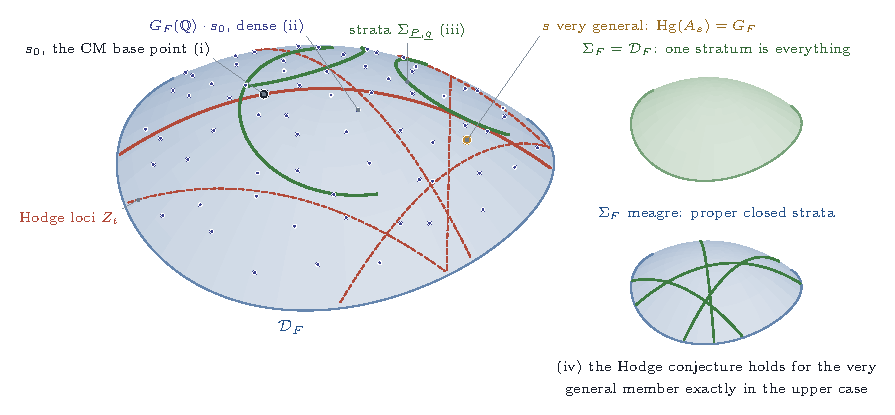
\includegraphics[width=\textwidth]{fig_mainlocus}
\caption{The algebraic locus of \Cref{thm:main}, drawn over a real slice of the
period domain $\cD_{F}$. Left: the explicit CM base point $s_{0}$ of part (i);
its Hecke orbit $G_{F}(\QQ)\cdot s_{0}$, which is dense by part (ii); three of
the strata $\Sigma_{\underline{P},\underline{q}}$ of part (iii), each closed
and algebraic, through points of the orbit; the Hodge loci $Z_{t}$, dashed,
one of them through $s_{0}$, off which the Hodge group of the member is all of
$G_{F}$ (\Cref{lem:cmgeneric}); and a very general point $s$. Right: the two
cases of the dichotomy of part (iii). By part (iv) the Hodge conjecture holds
for the very general member exactly in the upper case, where one stratum is
the whole domain.}
\label{fig:mainlocus}
\end{figure}


\subsection{The proof}

The first step is a base point. In \Cref{thm:cmbasepoint} the member $A_{s_{0}}$
is isogenous to $B_{\Phi}^{\,n}\times B_{\bbar\Phi}^{\,n}$, where $B_{\Phi}$ is
an abelian $m$-fold with complex multiplication by $F$ of a CM type determined
by the polarisation, and the Weil classes there are written out as
polynomials with rational coefficients in $F$-balanced divisor classes. For
an imaginary quadratic field $K$ there is a second base point in every family,
with quaternionic multiplication: whenever an algebra $(-d,b)_{\QQ}$ with
$b>0$ acts compatibly with $K$, the Weil line is spanned by the real and
imaginary parts of $\Theta^{n}$ for an explicit $(1,1)$ class $\Theta$, and
the discriminant of the family is the class of $b^{n}$, which can be any
discriminant (\Cref{thm:divcriterion}, \Cref{thm:quatweil},
\Cref{thm:everyfamily}). Products of abelian surfaces of Weil type give a
third, since the Weil class is multiplicative:
$\omega(A_{1})\,\omega(A_{2})=\omega(A_{1}\times A_{2})$ for the
$K$-valued Weil class $\omega$ (\Cref{thm:weilmult}, \Cref{thm:everyn}). None
of these base points uses anything beyond the theorem of Lefschetz on $(1,1)$
classes.

The second step moves the base point. An element of $G_{F}(\QQ)$, where
$G_{F}=\Res_{F_{0}/\QQ}\SU(V,H)$ and $F_{0}$ is the totally real subfield,
induces after clearing denominators an isogeny between two members and fixes
the Weil classes, so $\Sigma_{F}$ is a union of $G_{F}(\QQ)$-orbits
(\Cref{lem:Ginvariance}). The hermitian form is isotropic by the Hasse
principle, the rational points of the unipotent radicals of the parabolic
subgroups are dense in their real points, and these real points generate the
identity component of $G_{F}(\RR)$; so every orbit is dense
(\Cref{prop:densealg}, \Cref{thm:cmpropagation}(ii)).

The third step is properness. The relative Hilbert scheme of the universal
family, for one tuple of Hilbert polynomials, is proper over the Shimura
variety,%
\footnote{By Grothendieck's construction the Hilbert scheme of a projective
morphism, for a fixed Hilbert polynomial, is projective over the base; here
the base is the Shimura variety of the family, after a level structure that
makes the universal family exist, and the morphism is the universal abelian
scheme.}
and the class of a flat family of cycles is locally constant, so the
set of points at which a Weil class is represented by cycles with prescribed
Hilbert data is Zariski closed; $\Sigma_{F}$ is the countable union of these
strata (\Cref{thm:closedlocus}). The Baire category theorem then gives the
dichotomy of part (iii) (\Cref{cor:allornothing}). Part (iv) needs one more
fact, that the very general member has Hodge group $G_{F}$; we prove it
directly, from the simplicity of the real factors $\SU(n,n)$
(\Cref{lem:cmgeneric}, \Cref{cor:verygeneral}).

For an imaginary quadratic field everything can be written in coordinates.
On the standard model of \Cref{sec:explicit}, built from a $K$-vector space of
dimension $2n$ with a hermitian form of signature $(n,n)$, the Weil line has
the integral basis
\[
  \omega_{1}=\sum_{|T|\ \mathrm{even}}(-1)^{|T|/2}d^{\,n-|T|/2}\,w^{(T)},
  \qquad
  \omega_{2}=\sum_{|T|\ \mathrm{odd}}(-1)^{(|T|-1)/2}d^{\,n-(|T|+1)/2}\,w^{(T)},
\]
where $T$ runs over the subsets of $\{1,\dots,2n\}$ and $w^{(T)}$ is the
monomial taking $y_{j}$ for $j\in T$ and $x_{j}$ otherwise
(\Cref{thm:explicitgens}). A member with Hodge group $\SU(V,H)$ has exactly
three Hodge classes in degree $2n$ and one in every other degree
(\Cref{thm:hdgcount}), so the Hodge conjecture for it, in every degree at
once, is the algebraicity of the one class $\omega_{1}$, with $2^{2n-1}$
integer coefficients (\Cref{cor:whatisleft}). By Deligne's theorem
\cite{Del82} that class is absolutely Hodge at every point,%
\footnote{A class is absolutely Hodge if its image under every automorphism
$\sigma$ of $\CC$, through the comparison of Betti cohomology with
algebraic de Rham cohomology of the conjugate variety $X^{\sigma}$, is again
a Hodge class. Algebraic classes have this property, so it is a necessary
condition for algebraicity; Deligne proved it for every Hodge class on an
abelian variety.}
and the Hodge
conjecture for the family is equivalent to its algebraicity at every point of
one connected domain (\Cref{cor:exactform}).


\subsection{The classical constructions}

\Cref{sec:characters,sec:fm,sec:divisor,sec:numerology,sec:semireg,sec:hyperplane,sec:ks,sec:reduction,sec:escape} explain why two classical lines of attack do not
produce Weil classes, and the explanations are different in kind. The first
imports an object from a projective space, restricts it to the dual abelian
variety and transports it back by the Fourier--Mukai transform. Its Chern
character stays in the subring generated by the polarisation
(\Cref{thm:divisor}), because the cohomological transform carries powers of
the dual polarisation to rational multiples of powers of the polarisation in
closed form (\Cref{thm:fmtheta}); and a construction equivariant for the
field lands in the isotypic component of the norm character, which the Weil
line misses, since it sits at the two ends of the grading
(\Cref{thm:character}). The second is induction on dimension through
hyperplane sections, and the restriction map kills every primitive class of
middle degree (\Cref{thm:hyperplane}); below the middle degree the return
trip is the Lefschetz standard conjecture (\Cref{thm:returntrip}). The
Kuga--Satake construction, which changes the variety rather than cutting it,
reaches the Weil line only in dimension two (\Cref{prop:normpart}).%
\footnote{The construction attaches to a polarised Hodge structure $T$ of
weight two with $h^{2,0}=1$ an abelian variety $A$ with
$H^{1}(A,\QQ)=C^{+}(T)$, the even Clifford algebra, and an embedding of
$T$ into $\End(H^{1}(A,\QQ))$ by Hodge structures, which is a Hodge class on
the product of a variety carrying $T$ with $A\times A$; the Kuga--Satake
Hodge conjecture asks that this class be algebraic.} A rational
class of the Weil line has a $\Kx$-orbit spanning a plane, so any
construction reaching it must be bilinear in a pair of inputs exchanged by
$\Gal(K/\QQ)$ (\Cref{prop:orbitplane}), and Markman's construction is of that
kind.


\subsection{The companion papers}

By \Cref{thm:main}(iv) the Hodge conjecture for the very general member of a
Weil family is the closedness of $\Sigma_{F}$, and by (iii) it is enough to
show that one stratum has an interior point. Two statements would do this.
The first bounds the Hilbert data of the cycles along the orbit of the base
point (\Cref{thm:degreebound}); it is equivalent to its conclusion
(\Cref{thm:p1equivalent}), and it is needed only along one sequence of CM
points that leaves every proper special subvariety, which exists in the
orbit (\Cref{thm:escape}). The second is semiregularity: a perfect complex
at one base point whose Chern character is a nonzero multiple of a Weil
class plus a polynomial in the polarisation, and whose semiregularity map is
injective, extends along the whole family. The companion paper
\cite{paperII} proves this (\cite[Theorem~2.3]{paperII}), computes the
injectivity condition as one number, shows that it is never met when the
Chern character is exactly a Weil class, for any CM field, computes it
exactly for quartic CM fields, examines the secant objects of the split
member, the convolutions of line bundles and the supports of a complex
meeting the criterion. The companion paper \cite{paperIII} shows that the
Hodge conjecture is equivalent to two statements about algebraic loci, one on
abelian varieties and one on the classes reached from them by
correspondences, proves each where it can be proved, and proves the
conjecture itself for the very general complete intersection of diagonal
quadrics of Vandermonde type. The annihilator computation of
\Cref{sec:semireg}, which shows that no object on which $H^{2}(\cO_{A})$ acts
faithfully is semiregular, is the first step of that analysis and is proved
here because it uses only the explicit form of the classes.

Every proof is written to be checked by hand. Where an argument rests on a
finite calculation, the calculation is given where it is used, as an explicit
identity, a determinant or a case analysis. The archive \cite{BMB26} holds
programs that repeat much of this arithmetic and a Lean~4 certificate of
part of it; no statement of the paper rests on them.

\section{Conventions}\label{sec:conventions}
\enlargethispage{3pt}

All varieties are over $\CC$ and all cohomology is singular cohomology with
the indicated coefficients. For a smooth projective variety $X$ we write
$H^{p,q}(X)$ for the Hodge components of $H^{p+q}(X,\CC)$, and
\[
  \Hdg^{p}(X)=H^{2p}(X,\QQ)\cap H^{p,p}(X)
\]
for the space of rational Hodge classes of type $(p,p)$. A class is
\emph{algebraic} if it lies in the image of the cycle class map
$\cl^{p}_{X}\colon\CH^{p}(X)_{\QQ}\to\Hdg^{p}(X)$. The algebraic classes form
a subring of $H^{*}(X,\QQ)$, because the cycle class map carries intersection
products to cup products.%
\footnote{The intersection product on $\CH^{*}(X)_{\QQ}$ is defined because
$X$ is smooth, and its compatibility with the cycle class map is proved in
\cite[Chapter~19]{Ful98}. The integral form of the question, with $\ZZ$ in
place of $\QQ$, is a different problem and is not considered in this paper.}

An abelian variety $A$ of dimension $g$ has $H^{1}(A,\QQ)$ of dimension $2g$
and a canonical isomorphism
\begin{equation}\label{eq:wedge}
  H^{k}(A,\QQ)\;\cong\;\textstyle\bigwedge^{k}H^{1}(A,\QQ)
\end{equation}
of Hodge structures, with the cup product on the left corresponding to the
wedge product on the right. We use \eqref{eq:wedge} without further comment;
it is what makes every computation below finite.%
\footnote{Topologically $A=V/\Lambda$ is a real torus of dimension $2g$, so
$H^{*}(A,\ZZ)=\bigwedge^{*}\Hom(\Lambda,\ZZ)$ by the K\"unneth formula for
$(S^{1})^{2g}$, with the cup product corresponding to the wedge product. The
Hodge decomposition of $H^{k}$ is the $k$-th exterior power of
$H^{1}=H^{1,0}\oplus H^{0,1}$, because the translation-invariant forms
$dz_{I}\wedge d\bbar z_{J}$ are harmonic for the flat metric and represent
every class.}
The dual abelian variety is $\Av=\Pic^{0}(A)$, and
$H^{1}(\Av,\QQ)\cong H^{1}(A,\QQ)^{\vee}$.

A polarisation of $A$ is a class $\theta\in\NS(A)\otimes\QQ$ that is ample;
equivalently, an alternating form $E$ on $H_{1}(A,\QQ)$ satisfying the Riemann
relations. The polarisation is principal when $E$ is unimodular on
$H_{1}(A,\ZZ)$, and then $\theta^{g}/g!$ is the class of a point. We write
$\theta'$ for the polarisation on $\Av$ induced by $\theta$ through the
isogeny $\phi_{\theta}\colon A\to\Av$; when $\theta$ is principal,
$\phi_{\theta}$ is an isomorphism and $\phi_{\theta}^{*}\theta'=\theta$.

For an endomorphism $f$ of $A$ we write $f^{*}$ for the induced map on
cohomology. When a field $K$ acts on $A$ through
$\iota\colon K\hookrightarrow\End^{0}(A)=\End(A)\otimes\QQ$, each $\tau\in K$
acts on $H^{*}(A,\QQ)$ through $\iota(\tau)$, and we speak of the action of
$\tau$ when $\iota$ is understood. For nonzero $\tau$ in the order
$\iota^{-1}(\End(A))$ the element $\iota(\tau)$ is an isogeny; every element
of $K$ is a rational multiple of an element of this order, so the general
case follows by $\QQ$-linearity, and no statement below depends on the
distinction.

The Chern character of a bounded complex $\cE^{\bullet}$ of locally free
sheaves is $\ch(\cE^{\bullet})=\sum_{i}(-1)^{i}\ch(\cE^{i})$. On a smooth
projective variety every bounded complex of coherent sheaves is
quasi-isomorphic to such a complex, and the resulting class depends only on
the object of $D^{b}$. We write $\ch_{k}$ for the component in $H^{2k}$.
On an abelian variety the tangent bundle is trivial, and so is the Todd
class. Grothendieck--Riemann--Roch therefore reads
$\ch(f_{!}x)=f_{*}\ch(x)$ for a morphism $f$ between abelian varieties, and
$\ch\colon K_{0}(A)_{\QQ}\to\CH^{*}(A)_{\QQ}$ is an isomorphism of rings
\cite[Chapter~15]{Ful98}; both facts are used without further mention. For
the inclusion of a smooth subvariety, whose normal bundle need not be
trivial, the Todd class of the normal bundle enters, and it is written out
where it matters.

For the Fourier--Mukai transform we follow \cite{Muk81}. The Poincar\'e bundle
$\cP$ on $A\times\Av$ is normalised so that $\cP|_{A\times\{0\}}$ and
$\cP|_{\{0\}\times\Av}$ are trivial. With $p\colon A\times\Av\to A$ and
$q\colon A\times\Av\to\Av$ the projections, the transform is
\[
  \Phi_{\cP}\colon D^{b}(\Av)\to D^{b}(A),
  \qquad
  \Phi_{\cP}(\cG)=Rp_{*}\bigl(Lq^{*}\cG\otimes^{L}\cP\bigr).
\]
On cohomology we write the induced map with the same symbol,
\[
  \Phi_{\cP}\colon H^{*}(\Av,\QQ)\longrightarrow H^{*}(A,\QQ),
  \qquad
  \Phi_{\cP}(x)=p_{*}\bigl(q^{*}x\cdot\ch(\cP)\bigr),
\]
and the Grothendieck--Riemann--Roch theorem gives
$\ch(\Phi_{\cP}(\cG))=\Phi_{\cP}(\ch(\cG))$ because the Todd class of an
abelian variety is trivial; see \Cref{prop:grr}.

For an imaginary quadratic field $K$ we write $\Nm=\Nm_{K/\QQ}$ for the norm
and $\bbar{\tau}$ for the conjugate of $\tau\in K$. Characters of $\Kx$ are
written multiplicatively, and $\Nm^{n}$ denotes $\tau\mapsto\Nm(\tau)^{n}$.

Finally, we say that a construction is \emph{of ambient type} if it has the
shape of the hypothesis of \Cref{thm:divisor}: a morphism
$i\colon\Av\to\PP^{N-1}$ defined by a linear system, an object $\cF$ of
$D^{b}(\PP^{N-1})$, and the class $\ch_{k}(\Phi_{\cP}(Li^{*}\cF))$. Nothing is
assumed about $\cF$: it may be the structure sheaf of a secant variety, of a
join, of a determinantal locus or of any other subscheme, and it may be
twisted by any line bundle from the ambient space.

\section{Abelian varieties of Weil type}\label{sec:weiltype}

We fix the notion of Weil type, construct the Weil line, prove that it
consists of Hodge classes, and record the two facts about it that the
obstruction theorems use: its dimension, and its position relative to the
subring generated by divisor classes. The standard references are \cite{BL04}
for abelian varieties and \cite{Voi02} for Hodge theory. Apart from the
Riemann relations, the Lefschetz theorem on $(1,1)$ classes and the
description of the N\'eron--Severi group by symmetric endomorphisms, every
result of the section is proved here or in \Cref{sec:characters}.

\subsection{Weil type}

Let $K=\QQ(\sqrt{-d})$ be an imaginary quadratic field, with $d$ a squarefree
positive integer, and let $\bbar{\phantom{x}}$ denote the nontrivial element
of $\Gal(K/\QQ)$.

\begin{definition}[Weil type]\label{def:weiltype}
Let $A$ be a complex abelian variety, let
$\iota\colon K\hookrightarrow\End^{0}(A)$ be an embedding, and let $\eta$ be a
polarisation class on $A$. The triple $(A,\iota,\eta)$ is of
\emph{$(K,-1,n)$-Weil type} if
\begin{enumerate}[label=\textup{(\roman*)},nosep]
\item $\dim A=2n$;
\item the endomorphism $\iota(\sqrt{-d})$ acts on the tangent space
  $H^{0}(A,\Omega^{1}_{A})^{\vee}\cong H^{1,0}(A)^{\vee}$ with the two
  eigenvalues $\pm\sqrt{-d}$ each occurring with multiplicity $n$;
\item the Rosati involution attached to $\eta$ restricts on
  $\iota(K)\subset\End^{0}(A)$ to complex conjugation, that is
  $\iota(\tau)^{\dagger}=\iota(\bbar{\tau})$ for all $\tau\in K$.
\end{enumerate}
\end{definition}

Condition (ii) is the balanced signature condition. It separates Weil type
from the unbalanced case, in which the eigenvalues $\pm\sqrt{-d}$ occur with
different multiplicities, and it is the condition under which the Weil line
consists of Hodge classes (\Cref{rem:balancecount}). Condition (iii) says that
the polarisation is compatible with the $K$-action, and the middle entry $-1$
of $(K,-1,n)$ records the sign in this compatibility: the Rosati involution
restricts to conjugation on $\iota(K)$, not to the identity. By
\Cref{lem:rosatiauto} the sign is forced once $\iota(K)$ is stable under the
Rosati involution. Some authors suppress the sign and speak of $K$-Weil type
of dimension $2n$.

\begin{lemma}[$H^{1}$ is a $K$-space]\label{lem:Kspace}
Let $(A,\iota,\eta)$ be of $(K,-1,n)$-Weil type and put $V=H^{1}(A,\QQ)$. Then
$\iota$ makes $V$ a $K$-vector space of dimension $2n$, and
$\dim_{\QQ}V=4n$.
\end{lemma}

\begin{proof}
The algebra $\End^{0}(A)$ acts $\QQ$-linearly on $V$ by pullback. Pullback
reverses the order of composition, but $K$ is commutative, so
$\tau\mapsto\iota(\tau)^{*}$ is a unital ring homomorphism
$K\to\End_{\QQ}(V)$. Since $K$ is a field, $V$ becomes a $K$-vector space,
and since $\dim_{\QQ}V=2\dim A=4n$, we get $\dim_{K}V=4n/[K:\QQ]=2n$.
\end{proof}

\begin{notation}\label{not:eigen}
Write $V_{\CC}=V\otimes_{\QQ}\CC$. Since $\iota(\sqrt{-d})^{2}=-d$ on $V$,
the operator $\iota(\sqrt{-d})\otimes1$ on $V_{\CC}$ has the two
eigenvalues $\pm\sqrt{-d}$, and
\begin{equation}\label{eq:Vsplit}
  V_{\CC}=V_{+}\oplus V_{-},
  \qquad
  V_{\pm}=\ker\bigl(\iota(\sqrt{-d})\mp\sqrt{-d}\bigr),
\end{equation}
with $\dim_{\CC}V_{\pm}=2n$ each, because $V$ is free of rank $2n$ over $K$ and
$K\otimes_{\QQ}\CC\cong\CC\times\CC$. Complex conjugation on $V_{\CC}$, coming
from the real structure $V\otimes\RR$, interchanges $V_{+}$ and $V_{-}$. For
general $\tau=a+b\sqrt{-d}\in K$ the operator $\iota(\tau)$ acts on $V_{+}$ by
the scalar $\tau$ and on $V_{-}$ by $\bbar{\tau}$.
\end{notation}

\begin{remark}\label{rem:tautbar}
The two scalars in \Cref{not:eigen} are different functions of $\tau$. For
$\tau\notin\QQ$ the operator $\iota(\tau)$ is $\QQ$-linear on $V$ but not a
scalar; it becomes a scalar on each piece only after extension to $\CC$ and
splitting. This is the source of the characters studied in
\Cref{sec:characters}. A class defined over $\QQ$ can be an eigenvector of
every $\iota(\tau)$ only with an eigenvalue in $\QQ$; the function
$\Nm(\tau)=\tau\bbar{\tau}$ is $\QQ$-valued, and $\tau^{2n}$ is not
(\Cref{rem:rightcharacter}).
\end{remark}

\subsection{The Hodge structure}

Write the Hodge decomposition as $V_{\CC}=V^{1,0}\oplus V^{0,1}$, with
$V^{1,0}=H^{1,0}(A)$ and $V^{0,1}=H^{0,1}(A)$. The $K$-action preserves it,
because $\iota(\tau)$ is induced by an endomorphism of $A$ and is therefore a
morphism of Hodge structures. The eigenspaces of an operator that preserves
both summands are the direct sums of its eigenspaces on the two summands, so
each of $V_{+}$ and $V_{-}$ splits: with $V^{p,q}_{\pm}=V_{\pm}\cap V^{p,q}$,
\begin{equation}\label{eq:bisplit}
  V_{\pm}=V_{\pm}^{1,0}\oplus V_{\pm}^{0,1}.
\end{equation}

\begin{lemma}[Balanced signature]\label{lem:balanced}
For $(A,\iota,\eta)$ of $(K,-1,n)$-Weil type,
\[
  \dim_{\CC}V_{+}^{1,0}=\dim_{\CC}V_{-}^{1,0}=n,
  \qquad
  \dim_{\CC}V_{+}^{0,1}=\dim_{\CC}V_{-}^{0,1}=n .
\]
\end{lemma}

\begin{proof}
By \Cref{def:weiltype}(ii), $\iota(\sqrt{-d})$ acts on the tangent space with
each eigenvalue of multiplicity $n$. The tangent space is dual to
$H^{1,0}(A)=V^{1,0}$, and the action of $\iota(\sqrt{-d})$ on $V^{1,0}$ by
pullback is the transpose of its action on the tangent space, so it has the
same eigenvalues with the same multiplicities; that is,
$\dim V^{1,0}_{+}=\dim V^{1,0}_{-}=n$. Since $\dim_{\CC}V_{\pm}=2n$ by
\Cref{not:eigen} and $V_{\pm}=V^{1,0}_{\pm}\oplus V^{0,1}_{\pm}$, the
remaining two dimensions are $n$ each.
\end{proof}

\subsection{The Weil line}

\begin{definition}[Weil line]\label{def:weilline}
Let $(A,\iota,\eta)$ be of $(K,-1,n)$-Weil type and $V=H^{1}(A,\QQ)$. The
\emph{Weil line} is
\[
  \HW(A)\;=\;\Bigl(\textstyle\bigwedge^{2n}_{\CC}V_{+}\oplus
  \bigwedge^{2n}_{\CC}V_{-}\Bigr)\cap H^{2n}(A,\QQ),
\]
the intersection being taken inside
$H^{2n}(A,\CC)=\bigwedge^{2n}_{\CC}V_{\CC}$.
\end{definition}

\begin{proposition}[Structure of the Weil line]\label{prop:weilline}
Let $(A,\iota,\eta)$ be of $(K,-1,n)$-Weil type. Then
\begin{enumerate}[label=\textup{(\roman*)},nosep]
\item $\HW(A)$ is a $\QQ$-subspace of $H^{2n}(A,\QQ)$ of dimension $2$, stable
  under $\iota(K)$, and free of rank one as a $K$-module;
\item $\HW(A)\subset H^{n,n}(A)$, so every element of $\HW(A)$ is a Hodge class;
\item $\HW(A)$ is canonically isomorphic to $\bigwedge^{2n}_{K}V$ as a
  $K$-module.
\end{enumerate}
\end{proposition}

\begin{proof}
(i) Write $W_{\CC}=\bigwedge^{2n}V_{+}\oplus\bigwedge^{2n}V_{-}$. Each summand
is one-dimensional over $\CC$ because $\dim_{\CC}V_{\pm}=2n$, so
$\dim_{\CC}W_{\CC}=2$. The splitting \eqref{eq:Vsplit} is the eigenspace
decomposition of the operator $\iota(\sqrt{-d})$, which is defined over $\QQ$,
so every automorphism of $\CC$, acting on $V_{\CC}$ through the second
factor, either preserves $V_{+}$ and $V_{-}$ or interchanges them, according
to its restriction to $K$; complex conjugation interchanges them. Hence
$W_{\CC}$ is stable under $\mathrm{Aut}(\CC)$, and by Galois descent it is
defined over $\QQ$: the space $\HW(A)=W_{\CC}\cap H^{2n}(A,\QQ)$ has
$\dim_{\QQ}\HW(A)=2$ and $\HW(A)\otimes\CC=W_{\CC}$. It is stable under $\iota(K)$ because
$\iota(\tau)$ preserves each of $V_{\pm}$, hence each summand. A
two-dimensional $\QQ$-space with a faithful $K$-action is free of rank one
over $K$.

(ii) By \eqref{eq:bisplit} and \Cref{lem:balanced}, the line
$\bigwedge^{2n}V_{+}$ equals
$\bigwedge^{n}V^{1,0}_{+}\otimes\bigwedge^{n}V^{0,1}_{+}$, which is of Hodge
bidegree $(n,n)$. The same computation applies to $\bigwedge^{2n}V_{-}$.
Hence $W_{\CC}\subset H^{n,n}(A)$ and so
$\HW(A)\subset H^{2n}(A,\QQ)\cap H^{n,n}(A)=\Hdg^{n}(A)$.

(iii) Since $K\otimes_{\QQ}\CC\cong\CC\times\CC$, with the two factors
corresponding to the two embeddings of $K$, we have
$V\otimes_{\QQ}\CC=V\otimes_{K}(K\otimes_{\QQ}\CC)=V_{+}\oplus V_{-}$, and
exterior powers over $K$ commute with this base change:
\[
  \Bigl(\textstyle\bigwedge^{2n}_{K}V\Bigr)\otimes_{\QQ}\CC
  \;\cong\;\textstyle\bigwedge^{2n}_{\CC}V_{+}\oplus\bigwedge^{2n}_{\CC}V_{-}
  \;=\;W_{\CC}\;\subset\;H^{2n}(A,\CC).
\]
Every map in this chain is compatible with the action of $\mathrm{Aut}(\CC)$
through the second factor, which on the right permutes $V_{+}$ and $V_{-}$ as in (i).
By Galois descent the composite is induced by an injective $\QQ$-linear map
$\bigwedge^{2n}_{K}V\to H^{2n}(A,\QQ)$, which commutes with $\iota(K)$ because
each map in the chain does. Its image is a $\QQ$-subspace of
$W_{\CC}\cap H^{2n}(A,\QQ)=\HW(A)$ of dimension two, hence all of $\HW(A)$.
\end{proof}

\begin{remark}\label{rem:onedim}
Some authors call a generator of $\HW(A)$ \emph{the} Weil class and speak of a
one-dimensional space; the difference is the usual one between a $K$-line and
its underlying $\QQ$-plane. Nothing below depends on the convention, since
the obstruction theorems concern the whole of $\HW(A)$.
\end{remark}

\subsection{The Weil line and the divisor subring}

The Weil line is not accounted for by divisor classes. We record the
statement in the form in which it is used and derive it from the character
computation of \Cref{sec:characters}.

\begin{definition}\label{def:divisorsubring}
The \emph{divisor subring} $D^{*}(A)\subset H^{*}(A,\QQ)$ is the
$\QQ$-subalgebra generated by $\NS(A)\otimes\QQ\subset H^{2}(A,\QQ)$.
\end{definition}

Every element of $D^{*}(A)$ is algebraic, by the Lefschetz theorem on $(1,1)$
classes and the fact that the algebraic classes form a subring. The Hodge
conjecture for $A$ in degree $n$ is therefore equivalent to the algebraicity
of a complement of $D^{2n}(A)$ in $\Hdg^{n}(A)$. For a very general member of
a Weil family the Weil line is such a complement, by \Cref{thm:hdgcount}; at
special members the divisor subring can grow and meet the Weil line
(\cite[Remark~2.5]{paperIII}).

\begin{proposition}\label{prop:notpoly}
Let $(A,\iota,\eta)$ be of $(K,-1,n)$-Weil type with
$\End^{0}(A)=\iota(K)$, and suppose $n\ge1$. Then
\[
  \HW(A)\cap D^{2n}(A)=0 .
\]
\end{proposition}

\begin{proof}
By \Cref{prop:weilline}(i) and \Cref{thm:character}, the space
$\HW(A)\otimes\CC$ is the sum of the $\Kx$-eigenspaces for the characters
$\tau\mapsto\tau^{2n}$ and $\tau\mapsto\bbar{\tau}^{2n}$. The space
$\NS(A)\otimes\QQ$ is isomorphic to the space of elements of $\End^{0}(A)$
fixed by the Rosati involution \cite[Section~5.2]{BL04}. Since
$\End^{0}(A)=\iota(K)$ and the Rosati involution restricts to conjugation on
$\iota(K)$, the fixed elements are those of $\iota(\QQ)$, so
$\NS(A)\otimes\QQ=\QQ\,\eta$. By \Cref{lem:NSchar} the class $\eta$ is a
$\Kx$-eigenclass for the norm character $\Nm$, so every element of
$D^{2n}(A)=\QQ\,\eta^{n}$ is an eigenclass for $\Nm^{n}$. By
\Cref{lem:charsdiffer} the characters $\tau\mapsto\tau^{2n}$ and
$\tau\mapsto\bbar{\tau}^{2n}$ both differ from $\tau\mapsto\Nm(\tau)^{n}$.
Eigenvectors for pairwise distinct characters are linearly independent, so
$\HW(A)\otimes\CC$ meets the $\Nm^{n}$-eigenspace, which contains
$D^{2n}(A)$, only in zero.
\end{proof}

The mechanism behind the proof is that of \Cref{rem:rightcharacter}: $\Kx$
can act on a rational class through a character only if the character is
$\QQ$-valued, and the $\QQ$-valued characters occurring in the cohomology
are the powers of the norm. The Weil line has rank one over $K$, not over $\QQ$, and as a
$K$-line of exterior degree $2n$ it carries the $2n$-th power of $\tau$
itself. \Cref{thm:character} and \Cref{lem:NSchar,lem:charsdiffer} are proved
in \Cref{sec:characters}, and nothing there uses \Cref{prop:notpoly}, so the
forward reference is not circular.

\section{Weil classes in coordinates}\label{sec:explicit}

\Cref{sec:weiltype} defines the Weil line as an intersection inside
$H^{2n}(A,\CC)$. That description is convenient for proofs but exhibits no
single class, and in this section we write the Weil classes out. We build an
abelian variety of $(K,-1,n)$-Weil type from a $2n$-dimensional $K$-vector
space with a hermitian form, write two integral generators
$\omega_{1},\omega_{2}$ of the Weil line as sums of $2^{2n-1}$ monomials each,
and display them in full for $n=2$ and in a table for $n=3$. The coordinates
then give two things that the abstract description does not: an elementary
second proof that the Weil line misses the powers of the polarisation, and a
complete count of the Hodge classes in every degree, which reduces the Hodge
conjecture for a general member to the algebraicity of the single class
$\omega_{1}$.

\subsection{The standard model}

\begin{setupenv}[The model]\label{setup:model}
Fix a squarefree positive integer $d$, let $K=\QQ(\sqrt{-d})$, and fix the
embedding $K\hookrightarrow\CC$ carrying $\sqrt{-d}$ to $\delta:=i\sqrt{d}$.
Fix $n\ge1$ and let
\[
  V=K^{2n},
  \qquad
  u_{1},\dots,u_{2n}\ \text{the standard $K$-basis},
\]
regarded as a $\QQ$-vector space of dimension $4n$ with the basis
\[
  x_{j}:=u_{j},
  \qquad
  y_{j}:=\sqrt{-d}\,u_{j},
  \qquad 1\le j\le 2n .
\]
Let $S\colon V\to V$ be multiplication by $\sqrt{-d}$, so that in this basis
\begin{equation}\label{eq:Sbasis}
  S x_{j}=y_{j},
  \qquad
  S y_{j}=-d\,x_{j}.
\end{equation}
Let $\epsilon_{j}=-1$ for $1\le j\le n$ and $\epsilon_{j}=+1$ for
$n<j\le 2n$, and let $Q$ be the alternating $\QQ$-bilinear form on $V$ with
\begin{equation}\label{eq:Qbasis}
  Q(x_{j},y_{j})=\epsilon_{j},
  \qquad
  Q(x_{j},x_{k})=Q(y_{j},y_{k})=0,
  \qquad
  Q(x_{j},y_{k})=0 \ \ (j\ne k).
\end{equation}
Finally let $\eta\in\bigwedge^{2}V$ be the class with the same coefficients,
\begin{equation}\label{eq:etabasis}
  \eta=\sum_{j=1}^{2n}\epsilon_{j}\,x_{j}\wedge y_{j}.
\end{equation}
\end{setupenv}

Over $\CC$ the operator $S$ has the two eigenvalues $\pm\delta$, and its
eigenvectors can be written down directly.

\begin{lemma}[Eigenbasis]\label{lem:eigenbasis}
For $1\le j\le2n$ and $s\in\{+,-\}$ put
\begin{equation}\label{eq:eigenvec}
  u_{j}^{s}\;=\;\tfrac12\Bigl(x_{j}-s\,\tfrac{\delta}{d}\,y_{j}\Bigr)
  \ \in V_{\CC}.
\end{equation}
Then $S u_{j}^{s}=s\,\delta\,u_{j}^{s}$, the vectors $u_{1}^{+},\dots,u_{2n}^{+}$
form a basis of $V_{+}$ and $u_{1}^{-},\dots,u_{2n}^{-}$ a basis of $V_{-}$,
and complex conjugation on $V_{\CC}$ interchanges $u_{j}^{+}$ and $u_{j}^{-}$.
\end{lemma}

\begin{proof}
Using \eqref{eq:Sbasis} and $\delta^{2}=-d$,
\[
  S u_{j}^{s}
  =\tfrac12\bigl(y_{j}+s\,\tfrac{\delta}{d}\,d\,x_{j}\bigr)
  =\tfrac{s\delta}{2}\bigl(x_{j}+\tfrac{1}{s\delta}y_{j}\bigr)
  =\tfrac{s\delta}{2}\bigl(x_{j}-s\tfrac{\delta}{d}y_{j}\bigr)
  =s\,\delta\,u_{j}^{s},
\]
where the third equality uses $1/\delta=-\delta/d$. The change of basis
$(x_{j},y_{j})\mapsto(u_{j}^{+},u_{j}^{-})$ is block diagonal with
$2\times2$ blocks of determinant $\delta/(2d)\ne0$, so the $4n$ vectors
$u_{j}^{\pm}$ are linearly independent. Since $V_{+}$ and $V_{-}$ have
dimension $2n$ each by \Cref{not:eigen}, the $u_{j}^{+}$ form a basis of
$V_{+}$ and the $u_{j}^{-}$ a basis of $V_{-}$. Conjugation fixes $x_{j}$ and
$y_{j}$ and sends $\delta$ to $-\delta$, which interchanges the two formulas.
\end{proof}

\begin{definition}[The complex structure]\label{def:modelHS}
Define a Hodge structure of weight one on $V$ by
\begin{equation}\label{eq:V10}
  V^{1,0}
  =\bigl\langle u_{1}^{+},\dots,u_{n}^{+},\,
      u_{n+1}^{-},\dots,u_{2n}^{-}\bigr\rangle_{\CC},
  \qquad
  V^{0,1}=\overline{V^{1,0}} .
\end{equation}
\end{definition}

The first $n$ basis directions contribute to $V^{1,0}$ through their
$+$-eigenvector and the last $n$ through their $-$-eigenvector, so each of
$V_{\pm}$ meets $V^{1,0}$ in a subspace of dimension $n$. The signs
$\epsilon_{j}$ of \eqref{eq:Qbasis} are matched to this choice and are not
free: the proof of \Cref{thm:model} shows that the second Riemann relation
holds for them and fails as soon as one of them is reversed (see also
\Cref{rem:twosignatures}). Reversing all of them replaces $Q$ by $-Q$, and
the construction then goes through with $V^{1,0}$ and $V^{0,1}$ interchanged.

\begin{theorem}[The model is of Weil type]\label{thm:model}
With the data of \Cref{setup:model,def:modelHS}, the pair $(V,V^{1,0})$ is a
polarised rational Hodge structure of weight one with polarising form $Q$, so
$V=H^{1}(A,\QQ)$ for an abelian variety $A$ of dimension $2n$; the
multiplication $S$ makes $K$ act on $A$ up to isogeny; $\eta$ is the class of
the polarisation; and $(A,\iota,\eta)$ is of $(K,-1,n)$-Weil type in the sense
of \Cref{def:weiltype}.
\end{theorem}

\begin{proof}
We verify the two Riemann bilinear relations, then the three conditions of
\Cref{def:weiltype}.

\emph{The form vanishes on $V^{1,0}$.} By \eqref{eq:Qbasis} the form $Q$ is
block diagonal for the decomposition of $V$ into the planes
$\langle x_{j},y_{j}\rangle$, so $Q(u_{j}^{s},u_{k}^{t})=0$ whenever $j\ne k$.
Within one block, $Q(u_{j}^{s},u_{j}^{s})=0$ because $Q$ is alternating, and
\begin{equation}\label{eq:Qplusminus}
  Q(u_{j}^{+},u_{j}^{-})
  =\tfrac14\,Q\bigl(x_{j}-\tfrac{\delta}{d}y_{j},\;
                    x_{j}+\tfrac{\delta}{d}y_{j}\bigr)
  =\tfrac14\cdot\tfrac{2\delta}{d}\,Q(x_{j},y_{j})
  =\frac{\delta\,\epsilon_{j}}{2d}.
\end{equation}
The basis \eqref{eq:V10} of $V^{1,0}$ contains, for each $j$, exactly one of
$u_{j}^{+},u_{j}^{-}$. Hence any two of its members either lie in different
blocks or are equal, and in both cases $Q$ vanishes on them. So
$Q(V^{1,0},V^{1,0})=0$.

\emph{Positivity.} Let $0\ne v=\sum_{j}a_{j}v_{j}\in V^{1,0}$, where $v_{j}$ is
$u_{j}^{+}$ for $j\le n$ and $u_{j}^{-}$ for $j>n$. Then
$\bbar{v}=\sum_{j}\bbar{a_{j}}\,\bbar{v_{j}}$ with $\bbar{v_{j}}$ the other
eigenvector in the same block, so again only the diagonal terms survive:
\[
  i\,Q(v,\bbar{v})
  =\sum_{j\le n}i\,|a_{j}|^{2}\,Q(u_{j}^{+},u_{j}^{-})
   +\sum_{j>n}i\,|a_{j}|^{2}\,Q(u_{j}^{-},u_{j}^{+}) .
\]
By \eqref{eq:Qplusminus} and $\delta=i\sqrt{d}$ the first kind of term is
$i\cdot\delta\epsilon_{j}/(2d)=-\epsilon_{j}/(2\sqrt{d})$ and the second is
$+\epsilon_{j}/(2\sqrt{d})$. With $\epsilon_{j}=-1$ for $j\le n$ and $+1$ for
$j>n$ both are $+1/(2\sqrt{d})$, so $i\,Q(v,\bbar{v})=\|a\|^{2}/(2\sqrt{d})>0$.
This is the second Riemann relation. For the complex structure
\eqref{eq:V10} it forces the signature of $\epsilon$ to be $(n,n)$, since
reversing any single $\epsilon_{j}$ makes the corresponding term negative.

\emph{Weil type.} Condition (i) is $\dim A=\tfrac12\dim_{\QQ}V=2n$. For (ii),
$V^{1,0}$ is spanned by the $u_{j}^{+}$ with $j\le n$ and the $u_{j}^{-}$ with
$j>n$, so $\dim V^{1,0}_{+}=\dim V^{1,0}_{-}=n$; by duality, as in the proof
of \Cref{lem:balanced}, this is the balanced eigenvalue condition on the
tangent space. For (iii), write $\tau=a+b\sqrt{-d}$, so that $\iota(\tau)$
acts by
\[
  x_{j}\longmapsto a\,x_{j}+b\,y_{j},
  \qquad
  y_{j}\longmapsto -bd\,x_{j}+a\,y_{j},
\]
and $\iota(\bbar{\tau})$ by the same formulas with $b$ replaced by $-b$. Since
$Q$ is block diagonal and $\iota(\tau)$ preserves each block, it suffices to
compare $Q(\iota(\tau)v,w)$ with $Q(v,\iota(\bbar{\tau})w)$ for basis vectors
$v,w$ of one block, where
\begin{align*}
  Q\bigl(\iota(\tau)x_{j},y_{j}\bigr)&=a\epsilon_{j}
   =Q\bigl(x_{j},\iota(\bbar{\tau})y_{j}\bigr),\\
  Q\bigl(\iota(\tau)x_{j},x_{j}\bigr)&=-b\epsilon_{j}
   =Q\bigl(x_{j},\iota(\bbar{\tau})x_{j}\bigr),\\
  Q\bigl(\iota(\tau)y_{j},y_{j}\bigr)&=-bd\,\epsilon_{j}
   =Q\bigl(y_{j},\iota(\bbar{\tau})y_{j}\bigr),
\end{align*}
and the remaining pair $(y_{j},x_{j})$ follows from the first line with
$\tau$ replaced by $\bbar{\tau}$ and the antisymmetry of $Q$. So
$\iota(\tau)^{\dagger}=\iota(\bbar{\tau})$. Equivalently, in the form used
later, $\iota(\tau)^{*}\eta=\Nm(\tau)\,\eta$: by \eqref{eq:eigenvec},
$x_{j}\wedge y_{j}=\tfrac{2d}{\delta}\,u_{j}^{+}\wedge u_{j}^{-}$, and
$\iota(\tau)$ multiplies $u_{j}^{+}\wedge u_{j}^{-}$ by $\tau\bbar{\tau}$.

Finally, $\eta$ is of type $(1,1)$, because each $x_{j}\wedge y_{j}$ is a
multiple of $u_{j}^{+}\wedge u_{j}^{-}$ and in each block one of
$u_{j}^{+},u_{j}^{-}$ lies in $V^{1,0}$ and the other in $V^{0,1}$. Since in
addition $\eta^{2n}\ne0$, the class $\eta$ is a polarisation class.
\end{proof}

\begin{lemma}[The hermitian form]\label{lem:hermform}
On the model of \Cref{setup:model} there is a unique $K$-hermitian form $H$ on
$V$, linear in the first variable, with
\begin{equation}\label{eq:QfromH}
  Q(v,w)=\tfrac12\Tr_{K/\QQ}\bigl(\delta^{-1}H(v,w)\bigr),
  \qquad\text{namely}\qquad
  H(v,w)=Q(\sqrt{-d}\,v,\,w)+\sqrt{-d}\,Q(v,w),
\end{equation}
and in the basis $u_{1},\dots,u_{2n}$ it is
$H=\mathrm{diag}(-\epsilon_{1},\dots,-\epsilon_{2n})$, of signature $(n,n)$.
\end{lemma}

\begin{proof}
$K$-linearity in the first variable is the computation
\[
  H(\sqrt{-d}v,w)=Q(-dv,w)+\sqrt{-d}\,Q(\sqrt{-d}v,w)=\sqrt{-d}\,H(v,w),
\]
and the hermitian symmetry $\overline{H(w,v)}=H(v,w)$ follows from
$Q(v,\sqrt{-d}\,w)=-Q(\sqrt{-d}\,v,w)$, which is condition (iii) of
\Cref{def:weiltype} for $\tau=\sqrt{-d}$. Multiplying by $\delta^{-1}$ and
taking the trace kills the first summand of \eqref{eq:QfromH}, since $Q$ is
$\QQ$-valued and $\Tr_{K/\QQ}(\delta^{-1})=0$, and doubles the second; this
gives $Q$. For uniqueness, if $H'$ is a second such form and
$z=H(v,w)-H'(v,w)$, then $\Tr_{K/\QQ}(\delta^{-1}z)=0$, and replacing $v$ by
$\sqrt{-d}\,v$ gives $\Tr_{K/\QQ}(z)=0$; together these force $z=0$. Finally
$H(u_{j},u_{j})=Q(y_{j},x_{j})=-\epsilon_{j}$ and
$H(u_{j},u_{k})=0$ for $j\ne k$, so the signature is the number of indices with
$\epsilon_{j}=-1$ against the number with $\epsilon_{j}=+1$, that is $(n,n)$.
\end{proof}

\begin{remark}\label{rem:twosignatures}
The two signatures that have appeared express the same condition. The hermitian
form $H$ has signature $(n,n)$ by \Cref{lem:hermform}, and the $K$-action on
the tangent space has eigenvalue multiplicities $(n,n)$ by
\Cref{def:weiltype}(ii). The positivity computation in the proof of
\Cref{thm:model} passes from one to the other: the sign $\epsilon_{j}$
decides both which eigenvector of the $j$-th block is holomorphic and the sign
of $H$ on that block.
\end{remark}

\begin{remark}\label{rem:lattice}
Taking the lattice $\cO^{2n}$ for an order $\cO\subset K$ and scaling $Q$ to be
integral on it produces an abelian variety and not only a Hodge structure.
Nothing below depends on the lattice, so we work with the rational Hodge
structure throughout. Varying \eqref{eq:V10} over the period domain of the
hermitian form gives the Weil family, of dimension $n^{2}$ inside the
$n(2n+1)$-dimensional moduli of principally polarised abelian $2n$-folds
(\Cref{prop:weildomain}).
\end{remark}

\subsection{The two generators}

\begin{notation}\label{not:wT}
For $T\subseteq\{1,\dots,2n\}$ write
\[
  w^{(T)}=w^{(T)}_{1}\wedge w^{(T)}_{2}\wedge\cdots\wedge w^{(T)}_{2n},
  \qquad
  w^{(T)}_{j}=
  \begin{cases}
    y_{j}, & j\in T,\\
    x_{j}, & j\notin T .
  \end{cases}
\]
The $2^{2n}$ elements $w^{(T)}$ are part of the monomial basis of
$\bigwedge^{2n}V$, which has dimension $\binom{4n}{2n}$; they are the
monomials that contain exactly one of $x_{j},y_{j}$ for each $j$.
\end{notation}

\begin{theorem}[The Weil line in coordinates]\label{thm:explicitgens}
Let $(A,\iota,\eta)$ be the model of \Cref{thm:model} and let
\begin{equation}\label{eq:omegagens}
  \omega_{1}=\sum_{\substack{T\subseteq\{1,\dots,2n\}\\ |T|\ \mathrm{even}}}
    (-1)^{|T|/2}\,d^{\,n-|T|/2}\;w^{(T)},
  \qquad
  \omega_{2}=\sum_{\substack{T\subseteq\{1,\dots,2n\}\\ |T|\ \mathrm{odd}}}
    (-1)^{(|T|-1)/2}\,d^{\,n-(|T|+1)/2}\;w^{(T)} .
\end{equation}
Then
\begin{enumerate}[label=\textup{(\roman*)},nosep]
\item $\omega_{1}$ and $\omega_{2}$ have integer coefficients and each has
  exactly $2^{2n-1}$ nonzero terms;
\item $\omega_{1},\omega_{2}$ is a $\QQ$-basis of the Weil line
  $\HW(A)$ of \Cref{def:weilline};
\item writing $\omega_{\pm}=u_{1}^{\pm}\wedge\cdots\wedge u_{2n}^{\pm}$ for the
  generators of $\bigwedge^{2n}V_{\pm}$,
  \[
    \omega_{+}+\omega_{-}=\frac{\omega_{1}}{2^{2n-1}d^{\,n}},
    \qquad
    \frac{\omega_{+}-\omega_{-}}{\delta}=-\frac{\omega_{2}}{2^{2n-1}d^{\,n}} ;
  \]
\item $\iota(\tau)^{*}\omega_{+}=\tau^{2n}\omega_{+}$ and
  $\iota(\tau)^{*}\omega_{-}=\bbar{\tau}^{\,2n}\omega_{-}$ for all
  $\tau\in\Kx$, so on the plane $\langle\omega_{1},\omega_{2}\rangle$ the
  element $\iota(\tau)$ acts by the $\QQ$-rational matrix of multiplication by
  $\tau^{2n}$ on $K$;
\item $\omega_{1}$ and $\omega_{2}$ are of Hodge type $(n,n)$, hence are Hodge
  classes.
\end{enumerate}
\end{theorem}

\begin{proof}
(iii) and (i). Expanding \eqref{eq:eigenvec} in the product defining
$\omega_{s}$ and collecting the monomials $w^{(T)}$,
\begin{equation}\label{eq:omegaexp}
  \omega_{s}
  =\frac{1}{2^{2n}}\sum_{T}\Bigl(-s\,\frac{\delta}{d}\Bigr)^{|T|}w^{(T)},
\end{equation}
because the factor from index $j$ contributes $x_{j}$ with coefficient $1/2$
and $y_{j}$ with coefficient $-s\delta/(2d)$, and the monomials $w^{(T)}$
appear in the order $j=1,\dots,2n$ with no reordering sign. Therefore
\[
  \omega_{+}+\omega_{-}
  =\frac{1}{2^{2n-1}}\sum_{|T|\ \mathrm{even}}\Bigl(\frac{\delta}{d}\Bigr)^{|T|}w^{(T)},
  \qquad
  \frac{\omega_{+}-\omega_{-}}{\delta}
  =-\frac{1}{2^{2n-1}}\sum_{|T|\ \mathrm{odd}}\frac{\delta^{|T|-1}}{d^{|T|}}\,w^{(T)} ,
\]
since the terms with $|T|$ odd cancel in the first sum and those with $|T|$
even in the second. Now
$\delta^{2m}=(-d)^{m}$, so for $|T|=2m$ the coefficient in the first sum is
$(-1)^{m}d^{-m}$, and for $|T|=2m+1$ the coefficient in the second is
$-(-1)^{m}d^{-m-1}$. Multiplying by $2^{2n-1}d^{\,n}$ clears denominators,
since $m\le n$ in the first case and $m+1\le n$ in the second, and gives
\eqref{eq:omegagens}. The term counts are
$\sum_{m}\binom{2n}{2m}=\sum_{m}\binom{2n}{2m+1}=2^{2n-1}$.

(ii). By (iii), $\omega_{1}$ and $\omega_{2}$ lie in
$\bigwedge^{2n}V_{+}\oplus\bigwedge^{2n}V_{-}$. They are fixed by complex
conjugation, which interchanges $\omega_{+}$ and $\omega_{-}$ by
\Cref{lem:eigenbasis} and sends $\delta$ to $-\delta$, and by (i) they have
rational coefficients. Hence they lie in
$\bigl(\bigwedge^{2n}V_{+}\oplus\bigwedge^{2n}V_{-}\bigr)\cap H^{2n}(A,\QQ)$,
which is $\HW(A)$ by \Cref{def:weilline} and has dimension two by
\Cref{prop:weilline}(i). They are linearly independent over $\CC$ since
$\omega_{+},\omega_{-}$ are, so they form a basis of $\HW(A)$.

(iv). The first two identities are immediate, since $\iota(\tau)$ multiplies
each of the $2n$ factors $u_{j}^{+}$ by $\tau$ and each $u_{j}^{-}$ by
$\bbar{\tau}$. For the last clause, by (iii) the space $\HW(A)\otimes\CC$ is
$\CC\omega_{+}\oplus\CC\omega_{-}$, on which $\iota(\tau)$ acts by
$\tau^{2n}$ and $\bbar{\tau}^{\,2n}$; so under the isomorphism
$\HW(A)\cong K$ of \Cref{prop:weilline}(iii) the action of $\iota(\tau)$ is
multiplication by $\tau^{2n}$, whose matrix in the basis
$\omega_{1},\omega_{2}$ has rational entries.

(v). By \eqref{eq:V10} the monomial $\omega_{+}=u_{1}^{+}\wedge\cdots\wedge
u_{2n}^{+}$ has $n$ factors in $V^{1,0}$, namely those with $j\le n$, and $n$
factors in $V^{0,1}$; so $\omega_{+}$ is of type $(n,n)$, and likewise
$\omega_{-}$. By (iii), so are $\omega_{1}$ and $\omega_{2}$.
\end{proof}

\begin{remark}[Balanced signature]\label{rem:balancecount}
The balanced condition enters the proof of \Cref{thm:explicitgens} only in
part (v). If \eqref{eq:V10} is replaced by a complex structure with
$\dim V^{1,0}_{+}=p$ and $\dim V^{1,0}_{-}=2n-p$, everything else being kept,
then $\omega_{+}$ has $p$ holomorphic factors and is of type $(p,2n-p)$, so
$\HW(A)$ is a rational sub-Hodge structure of $H^{2n}(A,\QQ)$ of type
$\{(p,2n-p),(2n-p,p)\}$, and it contains a nonzero Hodge class if and only if
$p=n$. The balanced signature
in \Cref{def:weiltype}(ii) is therefore the condition under which the Weil
line contains Hodge classes at all. \Cref{prop:signatureforced} proves this
for every abelian variety with a Rosati-stable action of $K$.
\end{remark}

\subsection{The case \texorpdfstring{$n=2$}{n=2}}

Here $\dim A=4$, $\dim_{\QQ}V=8$, $H^{4}(A,\QQ)$ has dimension
$\binom{8}{4}=70$, and each generator has $2^{3}=8$ terms. Writing the
monomials in the order $j=1,2,3,4$ as in \Cref{not:wT}, \eqref{eq:omegagens}
reads
\begin{align}
  \omega_{1}
  &= d^{2}\,x_{1}x_{2}x_{3}x_{4}
     \;-\;d\!\!\sum_{|T|=2}\!\!w^{(T)}
     \;+\;y_{1}y_{2}y_{3}y_{4},
     \label{eq:n2omega1}\\[2pt]
  \omega_{2}
  &= d\!\!\sum_{|T|=1}\!\!w^{(T)}
     \;-\;\sum_{|T|=3}\!\!w^{(T)} ,
     \label{eq:n2omega2}
\end{align}
with the wedge signs omitted. For $d=1$, written out in full,
\begin{align*}
  \omega_{1}
  &= x_{1}x_{2}x_{3}x_{4}
   -y_{1}y_{2}x_{3}x_{4}-y_{1}x_{2}y_{3}x_{4}-y_{1}x_{2}x_{3}y_{4}
   -x_{1}y_{2}y_{3}x_{4}-x_{1}y_{2}x_{3}y_{4}-x_{1}x_{2}y_{3}y_{4}\\
  &\qquad{}+y_{1}y_{2}y_{3}y_{4},\\
  \omega_{2}
  &= y_{1}x_{2}x_{3}x_{4}+x_{1}y_{2}x_{3}x_{4}+x_{1}x_{2}y_{3}x_{4}
     +x_{1}x_{2}x_{3}y_{4}\\
  &\qquad{}-y_{1}y_{2}y_{3}x_{4}-y_{1}y_{2}x_{3}y_{4}-y_{1}x_{2}y_{3}y_{4}
     -x_{1}y_{2}y_{3}y_{4} .
\end{align*}
The square of the polarisation is
$\eta^{2}=2\sum_{j<k}\epsilon_{j}\epsilon_{k}\,x_{j}y_{j}x_{k}y_{k}$,
a sum of six monomials, none of which is among the sixteen above;
\Cref{prop:disjoint} below shows that this separation holds in every
dimension. \Cref{fig:weilcoeff} arranges the sixteen monomials $w^{(T)}$ on
the vertices of the $4$-cube.

\subsection{The case \texorpdfstring{$n=3$}{n=3}}

Here $\dim A=6$, $\dim_{\QQ}V=12$, $H^{6}(A,\QQ)$ has dimension
$\binom{12}{6}=924$, and each generator has $2^{5}=32$ terms. The coefficients
depend only on $|T|$, so the two classes are recorded completely by
\Cref{tab:n3coeffs}.

\begin{table}[htbp]
\centering
\renewcommand{\arraystretch}{1.2}
\begin{tabular}{@{}cccc@{\hskip 2.4em}cccc@{}}
\toprule
\multicolumn{4}{c}{$\omega_{1}$} & \multicolumn{4}{c}{$\omega_{2}$}\\
\cmidrule(r{1.6em}){1-4}\cmidrule(l){5-8}
$|T|$ & terms & coefficient & at $d=2$ &
$|T|$ & terms & coefficient & at $d=2$\\
\midrule
$0$ & $1$  & $+d^{3}$ & $+8$  & $1$ & $6$  & $+d^{2}$ & $+4$\\
$2$ & $15$ & $-d^{2}$ & $-4$  & $3$ & $20$ & $-d$     & $-2$\\
$4$ & $15$ & $+d$     & $+2$  & $5$ & $6$  & $+1$     & $+1$\\
$6$ & $1$  & $-1$     & $-1$  &     &      &          &     \\
\midrule
    & $32$ &          &       &     & $32$ &          &     \\
\bottomrule
\end{tabular}
\caption{The Weil classes at $n=3$. Each row gives the number of index sets
$T$ of that size and the common coefficient of the corresponding monomials
$w^{(T)}$ in \eqref{eq:omegagens}. The two classes together involve all $64$
monomials containing exactly one of $x_{j},y_{j}$ for each $j$, out of the
$924$ monomials of $H^{6}$.}
\label{tab:n3coeffs}
\end{table}

The pattern has a closed description. By \Cref{thm:explicitgens}(iii) and
\eqref{eq:eigenvec},
\begin{equation}\label{eq:omegaprod}
  \omega_{1}+\delta\,\omega_{2}
  =2^{2n}d^{\,n}\,\omega_{-}
  =d^{-n}\prod_{j=1}^{2n}\bigl(d\,x_{j}+\delta\,y_{j}\bigr),
\end{equation}
the product being the wedge product taken in the order $j=1,\dots,2n$. The
proof of \Cref{thm:explicitgens} uses of the basis only that the $u_{j}$ form
a $K$-basis of $V$, so \eqref{eq:omegagens} and \eqref{eq:omegaprod} define
generators of the Weil line, and hold, for every $K$-basis $u_{1},\dots,u_{2n}$
of $H^{1}(A,\QQ)$ of an abelian variety of $(K,-1,n)$-Weil type, with
$x_{j}=u_{j}$ and $y_{j}=\sqrt{-d}\,u_{j}$. For
$n=3$ and $d=1$ the coefficients in \Cref{tab:n3coeffs} are $+1,-1,+1,-1$
for $\omega_{1}$ and $+1,-1,+1$ for $\omega_{2}$, and the two classes are the
real and imaginary parts of $\prod_{j=1}^{6}\bigl(x_{j}+\sqrt{-1}\,y_{j}\bigr)$.

\begin{figure}[htbp]
\centering
  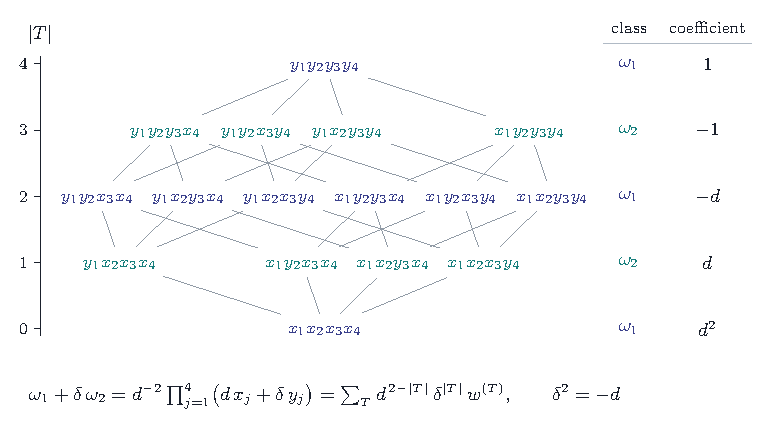
\includegraphics[width=0.78\textwidth]{fig_weilcube}
\caption{The $2^{2n}=16$ monomials $w^{(T)}$ of \Cref{not:wT} at $n=2$, as the
vertices of the $4$-cube, projected so that the height of $w^{(T)}$ is
$\lvert T\rvert$. An edge joins two monomials whose index sets differ in one
element, that is, two monomials related by a single substitution
$x_{j}\mapsto y_{j}$. The two colours are the bipartition by the parity of
$\lvert T\rvert$: the eight even vertices carry $\omega_{1}$ and the eight odd
ones carry $\omega_{2}$. The coefficient of $w^{(T)}$ depends only on
$\lvert T\rvert$ and is given by \eqref{eq:n2omega1} and
\eqref{eq:n2omega2}.}
\label{fig:weilcoeff}
\end{figure}

\subsection{Disjoint supports}

\Cref{prop:notpoly} is deduced from the character computation of
\Cref{sec:characters}. In the model the Weil line can be separated from the
powers of the polarisation without any representation theory: the Weil
classes and the powers of $\eta$ are supported on disjoint sets of monomials.

\begin{proposition}[Disjoint supports]\label{prop:disjoint}
In the model of \Cref{thm:model}, every monomial occurring in $\omega_{1}$ or
in $\omega_{2}$ contains exactly one of $x_{j},y_{j}$ for every
$j\in\{1,\dots,2n\}$, and every monomial occurring in $\eta^{k}$ contains
either both or neither, for every $j$ and every $k\ge0$. Consequently
\[
  \HW(A)\cap\QQ\,\eta^{n}=0 ,
\]
and more generally $\HW(A)$ meets the span of the monomials occurring in
powers of $\eta$ in zero.
\end{proposition}

\begin{proof}
The first assertion holds by \eqref{eq:omegagens} and \Cref{not:wT}. For the
second, $\eta$ is the combination \eqref{eq:etabasis} of the $2n$ two-forms
$x_{j}\wedge y_{j}$, which pairwise commute and square to zero, so
\[
  \eta^{k}=k!\sum_{\substack{S\subseteq\{1,\dots,2n\}\\|S|=k}}
    \Bigl(\prod_{j\in S}\epsilon_{j}\Bigr)\,
    \bigwedge_{j\in S}\bigl(x_{j}\wedge y_{j}\bigr),
\]
and the monomial indexed by $S$ contains both $x_{j}$ and $y_{j}$ for $j\in S$
and neither for $j\notin S$. A monomial cannot satisfy both patterns for a
given $j$, and since $2n\ge1$ there is at least one index at which to test,
so the two families of monomials are disjoint. Since
$\omega_{1},\omega_{2}$ span $\HW(A)$ by \Cref{thm:explicitgens}(ii), a nonzero
element of $\HW(A)$ has a nonzero coefficient on some $w^{(T)}$. As the
monomials form a basis of $\bigwedge^{2n}V$ and $w^{(T)}$ occurs in no power
of $\eta$, such an element does not lie in the span of the monomials
occurring in powers of $\eta$, and in particular not in $\QQ\,\eta^{n}$.
\end{proof}

\begin{remark}\label{rem:twoproofs}
The two proofs that the Weil line misses the powers of the polarisation
differ in scope. \Cref{prop:disjoint} concerns one model and one basis, and it
is short because the basis makes the $K$-action block diagonal. The
character proof is basis free, applies to every abelian variety of Weil type,
and identifies the obstruction as a difference of characters. The first can
be checked by hand; the second is the argument that \Cref{thm:character}
extends.
\end{remark}

\subsection{The Hodge ring of a general member}

It remains to count the Hodge classes, which measures how much of the Hodge
conjecture for $A$ is at stake. The Hodge classes of an abelian variety are
the invariants of its Hodge group, the special Mumford--Tate group
$\Hg(A)\subseteq\SL(V)$ \cite{Del82}:
$\Hdg^{k}(A)=H^{2k}(A,\QQ)^{\Hg(A)}$.

\begin{lemma}[The Hodge group]%
\label{lem:HgSU}
Let $(A,\iota,\eta)$ be of $(K,-1,n)$-Weil type and let $H$ be the
$K$-hermitian form of \Cref{lem:hermform}. Then
\[
  \Hg(A)\subseteq\SU(V,H) .
\]
\end{lemma}

\begin{proof}
The group $\Hg(A)$ is a $\QQ$-algebraic subgroup of $\SL(V)$ which fixes
every Hodge class in every tensor construction on $V$. It fixes
$\eta\in\bigwedge^{2}V$, hence preserves $Q$; and it commutes with $\iota(K)$,
because each $\iota(\tau)$ is a Hodge class in $V\otimes V^{\vee}$. A
$\QQ$-linear automorphism of $V$ commuting with the $K$-action and preserving
$Q$ preserves $H$, by the formula \eqref{eq:QfromH} expressing $H$ through $Q$
and the $K$-action. Hence $\Hg(A)\subseteq\mathrm{U}(V,H)$. Now
$\HW(A)$ consists of Hodge classes by \Cref{prop:weilline}(ii), so $\Hg(A)$
fixes $\HW(A)\otimes\CC$ pointwise, and in particular it fixes the line
$\bigwedge^{2n}V_{+}$ pointwise. An element $g\in\mathrm{U}(V,H)$ acts on
$\bigwedge^{2n}V_{+}$ by $\det_{K}(g)$,
so every $g\in\Hg(A)$ has $\det_{K}(g)=1$, which is the definition of
$\SU(V,H)$.
\end{proof}

For a very general member of the Weil family, that is, for every member whose
point in the period domain $\cD_{n,n}$ of \Cref{prop:weildomain} lies outside
a certain countable union of proper closed analytic subsets, the containment
of \Cref{lem:HgSU} is an equality; this is Weil's theorem \cite{Weil77}, in the
form given by Moonen and Zarhin \cite{MZ99}. The restriction to very general
members cannot be replaced by a Zariski open condition, since the locus where
the endomorphism algebra jumps is a countable union of such subsets, by
\Cref{thm:cdk}, and is dense in the classical topology. For such a member the
Hodge classes can be counted in every degree.

\begin{theorem}[The Hodge ring of a general member]\label{thm:hdgcount}
Let $(A,\iota,\eta)$ be of $(K,-1,n)$-Weil type with
$\Hg(A)=\SU(V,H)$. Then for every $k$ with $0\le k\le 2n$,
\[
  \dim_{\QQ}\Hdg^{k}(A)=
  \begin{cases}
    3, & k=n,\\[2pt]
    1, & k\ne n,
  \end{cases}
  \qquad\text{and}\qquad
  \Hdg^{n}(A)=\QQ\,\eta^{n}\oplus\HW(A).
\]
\end{theorem}

\begin{proof}
Complexify. The group $\SU(V,H)\otimes\CC$ is $\SL(V_{+})\cong\SL_{2n}(\CC)$,
acting on $V_{+}$ tautologically and on $V_{-}$ through the isomorphism
$V_{-}\cong V_{+}^{\vee}$ induced by $H$. By \Cref{prop:grading},
\[
  H^{2k}(A,\CC)=\bigoplus_{r+s=2k}
    \textstyle\bigwedge^{r}V_{+}\otimes\bigwedge^{s}V_{+}^{\vee},
\]
so it suffices to find the invariants in each summand. An invariant is a
weight-zero vector annihilated by every raising operator. Fix a basis of
$V_{+}$, take the diagonal torus of $\SL(V_{+})$ as maximal torus, and for
$T,U\subseteq\{1,\dots,2n\}$ let $v_{T}\in\bigwedge^{|T|}V_{+}$ and
$v_{U}^{\vee}\in\bigwedge^{|U|}V_{+}^{\vee}$ be the corresponding monomials in
the basis and its dual. In the weight lattice of $\SL_{2n}$ the weight of
$v_{T}\otimes v_{U}^{\vee}$ is
$\mathbf{1}_{T}-\mathbf{1}_{U}$ modulo $(1,1,\dots,1)$; since the entries of
$\mathbf{1}_{T}-\mathbf{1}_{U}$ lie in $\{-1,0,1\}$, the only multiples of
$(1,\dots,1)$ it can equal are $0$ and $\pm(1,\dots,1)$, giving
\[
  T=U \quad(\text{so } r=s),
  \qquad
  (T,U)=\bigl(\{1,\dots,2n\},\emptyset\bigr),
  \qquad
  (T,U)=\bigl(\emptyset,\{1,\dots,2n\}\bigr).
\]
The last two occur only for $(r,s)=(2n,0)$ and $(0,2n)$, each with a
one-dimensional weight-zero space consisting of the invariant lines
$\bigwedge^{2n}V_{+}$ and $\bigwedge^{2n}V_{-}$, which are $\SL$-invariant
because $\SL$ has trivial determinant. For $r=s$ the weight-zero space has
dimension $\binom{2n}{r}$ and its invariant subspace is the line spanned by the
image of the identity under
$\End(\bigwedge^{r}V_{+})\cong\bigwedge^{r}V_{+}\otimes\bigwedge^{r}V_{+}^{\vee}$,
which is one dimensional because $\bigwedge^{r}V_{+}$ is an irreducible
$\SL_{2n}$-module and Schur's lemma applies.

Collecting the contributions: for $k\ne n$ the only one is $(r,s)=(k,k)$, of
dimension one and spanned by $\eta^{k}$, which is a nonzero invariant lying in
that summand by \Cref{lem:NSchar}. For $k=n$ there are three contributions,
$(n,n)$, $(2n,0)$ and $(0,2n)$, of total dimension three; the first is spanned
by $\eta^{n}$ and the last two span $\HW(A)\otimes\CC$ by \Cref{lem:weilchar}.
Taking invariants commutes with extension of scalars from $\QQ$ to $\CC$, so
the dimensions over $\QQ$ are the same.
\end{proof}

\Cref{fig:hodgespike} displays these dimensions for $n=2,3,4$.

\begin{corollary}[Reduction to one class]\label{cor:whatisleft}
Let $(A,\iota,\eta)$ be as in \Cref{thm:hdgcount}. The Hodge conjecture holds
for $A$ in every degree if and only if the single class $\omega_{1}$ of
\eqref{eq:omegagens} is algebraic.
\end{corollary}

\begin{proof}
For $k\ne n$ the Hodge classes are the multiples of $\eta^{k}$, which are
algebraic, being powers of a divisor class. For $k=n$ they are spanned by
$\eta^{n}$, $\omega_{1}$ and $\omega_{2}$ by \Cref{thm:hdgcount}. Finally,
$\omega_{2}$ is algebraic as soon as $\omega_{1}$ is. By
\Cref{thm:explicitgens}(iv) the plane $\HW(A)$ is a free $K$-module of rank one
generated by $\omega_{1}$. For $\tau\in\Kx$ some positive integer multiple
$m\,\iota(\tau)$ lies in $\End(A)$, and on $H^{2n}(A,\QQ)$ the operator
$\iota(\tau)^{*}$ is $m^{-2n}$ times the pullback by $m\,\iota(\tau)$, so it
carries algebraic classes to algebraic classes. Any $\tau$ with
$\tau^{2n}\notin\QQ$, which exists by the argument of \Cref{lem:charsdiffer},
moves $\omega_{1}$ to a class with a nonzero $\omega_{2}$ component, and so
$\omega_{2}$ is a rational combination of the algebraic classes $\omega_{1}$
and $\iota(\tau)^{*}\omega_{1}$.
\end{proof}

\begin{remark}\label{rem:onlyoneclass}
\Cref{cor:whatisleft} explains why the Weil line is the standard test case. On a
general abelian variety of Weil type the Hodge conjecture concerns one
explicitly written class with $2^{2n-1}$ integer coefficients, and no space of
classes of unknown structure. The obstruction theorems of this paper
constrain the ways in which that class can be produced, and
\Cref{sec:basepoints} exhibits in every Weil family a member on which the
whole Weil line consists of polynomials in divisor classes.
\end{remark}

\begin{figure}[htbp]
\centering
  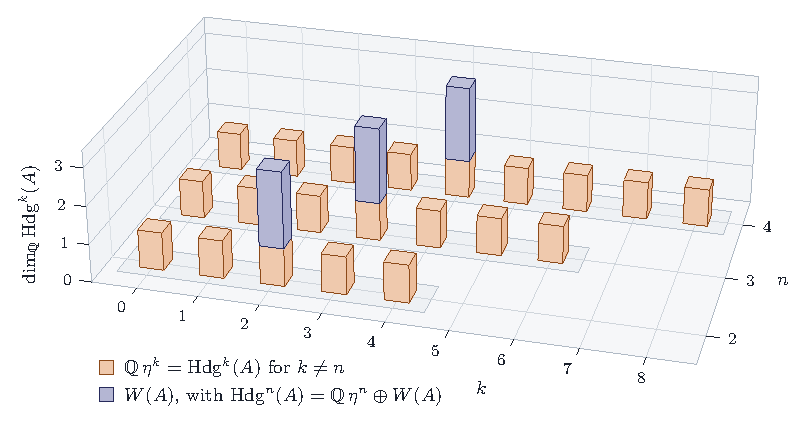
\includegraphics[width=0.9\textwidth]{fig_hodgespike}
\caption{The dimensions of $\Hdg^{k}(A)$ for a general abelian variety of
$(K,-1,n)$-Weil type, $0\le k\le 2n$, at $n=2,3,4$, as computed in
\Cref{thm:hdgcount}. Every degree carries the line $\QQ\,\eta^{k}$; the middle
degree $k=n$ carries in addition the two dimensions of the Weil line
$\HW(A)$, and nothing else occurs. The profile is the same for every $n$.}
\label{fig:hodgespike}
\end{figure}

\section{The character grading and the position of the Weil line}
\label{sec:characters}

This section proves the character obstruction, \Cref{thm:character}, which
is used in the proof of \Cref{prop:notpoly}. The group $\Kx$
acts on $H^{2n}(A,\QQ)$ through the endomorphisms $\iota(\tau)$. This action
grades the cohomology, and the Weil line and the power $\eta^{n}$ of the
polarisation lie in different graded pieces; once the grading is written
down, the obstruction follows in a few lines. The one point that needs care
is the character through which $\Kx$ acts on the Weil line. It is
$\tau\mapsto\tau^{2n}$, together with its conjugate, and not a power of the
norm, even though the Weil line is a $K$-line and multiplication by $\tau$ on
a $K$-line has determinant $\Nm(\tau)$ (\Cref{rem:failuremode}).

\subsection{The grading}

Throughout this section $(A,\iota,\eta)$ is of $(K,-1,n)$-Weil type,
$V=H^{1}(A,\QQ)$, and $V_{\CC}=V_{+}\oplus V_{-}$ is the splitting of
\Cref{not:eigen}.

\begin{proposition}[Character grading]\label{prop:grading}
For every $k\ge0$,
\begin{equation}\label{eq:grading}
  H^{k}(A,\CC)\;=\;\bigoplus_{r+s=k}
    \Bigl(\textstyle\bigwedge^{r}V_{+}\otimes\bigwedge^{s}V_{-}\Bigr),
\end{equation}
and $\iota(\tau)^{*}$ acts on the summand indexed by $(r,s)$ by the scalar
$\tau^{r}\bbar{\tau}^{\,s}$. The summands are the isotypic components for the
action of $\Kx$, and the characters $\tau\mapsto\tau^{r}\bbar{\tau}^{\,s}$ for
distinct pairs $(r,s)$ with $r+s=k$ are pairwise distinct.
\end{proposition}

\begin{proof}
By \eqref{eq:wedge}, $H^{k}(A,\CC)=\bigwedge^{k}V_{\CC}$, and the exterior
power of a direct sum decomposes as
$\bigwedge^{k}(V_{+}\oplus V_{-})=\bigoplus_{r+s=k}\bigwedge^{r}V_{+}\otimes\bigwedge^{s}V_{-}$,
which is \eqref{eq:grading}. By \Cref{not:eigen}, $\iota(\tau)^{*}$ acts on
$V_{+}$ by $\tau$ and on $V_{-}$ by $\bbar{\tau}$. Since it is an algebra
homomorphism for the wedge product, it acts on
$\bigwedge^{r}V_{+}\otimes\bigwedge^{s}V_{-}$ by $\tau^{r}\bbar{\tau}^{\,s}$.

For the last statement, suppose that
$\tau^{r}\bbar{\tau}^{\,s}=\tau^{r'}\bbar{\tau}^{\,s'}$ for all $\tau\in\Kx$,
where $r+s=r'+s'=k$. Then $s-s'=r'-r$, and dividing gives
$(\tau/\bbar{\tau})^{r-r'}=1$ for every $\tau\in\Kx$. If $r\ne r'$, the image
of the map $c(\tau)=\tau/\bbar{\tau}$ therefore lies in the group of
$(r-r')$-th roots of unity of $K$, which is finite: the group of all roots of
unity of the imaginary quadratic field $K$ has order $2$, $4$ or $6$. But $c$
has infinite image. Two elements have the same image exactly when their ratio
lies in $\QQ^{\times}$, and the elements $m+\sqrt{-d}$ with $m\in\ZZ$ are
pairwise non-proportional over $\QQ$. Hence $r=r'$, and so $s=s'$. Since the
characters of the summands are pairwise distinct, the summands are the
isotypic components.

The distinctness is that of characters of the torus
$\Res_{K/\QQ}\mathbb{G}_{m}$, not of their values at a given $\tau$: the
values at $\tau$ for $(r,s)$ and $(r',s')$ agree if and only if
$\tau/\bbar{\tau}$ is a root of unity of order dividing $r-r'$, and this can
happen (\Cref{rem:witness}).
\end{proof}

\begin{lemma}[The polarisation sits in the middle]\label{lem:NSchar}
Let $(A,\iota,\eta)$ be of $(K,-1,n)$-Weil type. Then
\[
  \iota(\tau)^{*}\eta=\Nm_{K/\QQ}(\tau)\,\eta\qquad\text{for all }\tau\in\Kx,
\]
so $\eta$ lies in the summand $(r,s)=(1,1)$ of \eqref{eq:grading} and
$\eta^{n}$ lies in the summand $(r,s)=(n,n)$, on which $\Kx$ acts by $\Nm^{n}$.
\end{lemma}

\begin{proof}
Let $E$ be the alternating form on $H_{1}(A,\QQ)$ attached to $\eta$. By
condition (iii) of \Cref{def:weiltype}, the Rosati involution $\dagger$ of
$\eta$ satisfies $\iota(\tau)^{\dagger}=\iota(\bbar{\tau})$, so by the
defining property of the Rosati involution
\[
  E\bigl(\iota(\tau)x,\,y\bigr)=E\bigl(x,\,\iota(\tau)^{\dagger}y\bigr)
  =E\bigl(x,\,\iota(\bbar{\tau})y\bigr)
  \qquad\text{for all }x,y .
\]
Therefore
\begin{align*}
  \bigl(\iota(\tau)^{*}E\bigr)(x,y)
  &=E\bigl(\iota(\tau)x,\iota(\tau)y\bigr)
   =E\bigl(x,\iota(\bbar{\tau})\iota(\tau)y\bigr)\\
  &=E\bigl(x,\iota(\Nm(\tau))y\bigr)=\Nm(\tau)\,E(x,y),
\end{align*}
using $\bbar{\tau}\tau=\Nm(\tau)\in\QQ$ and the $\QQ$-linearity of $\iota$.
Under the identification of $H^{2}(A,\QQ)=\bigwedge^{2}H^{1}(A,\QQ)$ with the
alternating forms on $H_{1}(A,\QQ)$, which is compatible with pullback, $\eta$
corresponds to $E$, so this is the displayed identity. Since
$\Nm(\tau)=\tau\bbar{\tau}$, \Cref{prop:grading} identifies the isotypic
component of $\Nm$ in $H^{2}(A,\CC)$ with the summand $(r,s)=(1,1)$, and
$\eta$ lies in it. Because $\iota(\tau)^{*}$ is a ring homomorphism,
$\iota(\tau)^{*}\eta^{n}=\Nm(\tau)^{n}\eta^{n}$, and in the same way this
places $\eta^{n}$ in the summand $(n,n)$.
\end{proof}

\begin{lemma}[The Weil line sits at the ends]\label{lem:weilchar}
Let $(A,\iota,\eta)$ be of $(K,-1,n)$-Weil type. Then
\[
  \HW(A)\otimes_{\QQ}\CC
  =\Bigl(\textstyle\bigwedge^{2n}V_{+}\Bigr)\oplus
   \Bigl(\textstyle\bigwedge^{2n}V_{-}\Bigr),
\]
the summands $(r,s)=(2n,0)$ and $(0,2n)$ of \eqref{eq:grading} in degree $2n$,
on which $\Kx$ acts by $\tau\mapsto\tau^{2n}$ and $\tau\mapsto\bbar{\tau}^{\,2n}$.
\end{lemma}

\begin{proof}
This is \Cref{def:weilline} together with \Cref{prop:weilline}(i), which says
that $\HW(A)$ is the $\QQ$-structure on that pair of lines; the characters are
read off from \Cref{prop:grading} with $(r,s)=(2n,0)$ and $(0,2n)$.
\end{proof}

\begin{lemma}[The two characters differ]\label{lem:charsdiffer}
For every $n\ge1$ the characters $\tau\mapsto\tau^{2n}$ and
$\tau\mapsto\Nm_{K/\QQ}(\tau)^{n}=(\tau\bbar{\tau})^{n}$ of $\Kx$ are distinct,
as are $\tau\mapsto\bbar{\tau}^{\,2n}$ and $\Nm^{n}$.
\end{lemma}

\begin{proof}
This is the case $(r,s)=(2n,0)$, $(r',s')=(n,n)$ of the last assertion of
\Cref{prop:grading}; we write the argument out in this case. For $\tau\ne0$
the identity $\tau^{2n}=(\tau\bbar{\tau})^{n}$ is equivalent to
$(\tau/\bbar{\tau})^{n}=1$, so the two characters agree if and only if
$(\tau/\bbar{\tau})^{n}=1$ for every $\tau\in\Kx$.

Consider the map $c\colon\Kx\to\Kx$, $c(\tau)=\tau/\bbar{\tau}$. Two elements
have the same image if and only if their ratio is fixed by conjugation, that
is, lies in $\QQ^{\times}$. The elements $m+\sqrt{-d}$ with $m\in\ZZ$ are
pairwise non-proportional over $\QQ$, so $c$ takes infinitely many values.

On the other hand, $\{\zeta\in K:\zeta^{n}=1\}$ is contained in the group
$\mu(K)$ of roots of unity of $K$, and for an imaginary quadratic field
$\mu(K)$ is finite: it has order $4$ for $d=1$, order $6$ for $d=3$, and order
$2$ otherwise. Since the image of $c$ is infinite, it is not contained in this
finite set, so some $\tau\in\Kx$ has $(\tau/\bbar{\tau})^{n}\ne1$, and the
characters differ. The second pair is obtained from the first by conjugation.
\end{proof}

\begin{remark}[Explicit witnesses]\label{rem:witness}
The proof does not exhibit a $\tau$ at which the two characters differ, and
the natural candidate $\tau=1+\sqrt{-d}$ is not always one. For $d=1$ its
ratio $\tau/\bbar{\tau}$ is $\sqrt{-1}$, a primitive fourth root of unity, so
the two characters agree at this $\tau$ whenever $4\mid n$; for $d=3$ the
ratio is $(-1+\sqrt{-3})/2$, a primitive cube root of unity, and they agree
whenever $3\mid n$. The candidate $\tau=3+\sqrt{-d}$ fails as well, at $d=3$
with $6\mid n$, where the ratio is $(1+\sqrt{-3})/2$, a primitive sixth root of
unity. In each case the characters agree at $\tau$ exactly when the order of
the ratio divides $n$. The element $\tau=2+\sqrt{-d}$ is a witness for every $d$
and every $n$. Its ratio is $\bigl(4-d+4\sqrt{-d}\bigr)/(4+d)$, which is not
$\pm1$, and for $d\notin\{1,3\}$ these are the only roots of unity in $K$;
for $d=1$ and $d=3$ the ratios $(3+4\sqrt{-1})/5$ and $(1+4\sqrt{-3})/7$ are
not roots of unity either, since their traces $6/5$ and $2/7$ are not
integers. The same holds for $4+\sqrt{-d}$ and $3+2\sqrt{-d}$. The finiteness
argument in the proof covers all fields at once and needs no witness. \Cref{fig:witness} shows the powers of these ratios for $d=1$ and $d=3$.
\end{remark}

\begin{figure}[htbp]
\centering
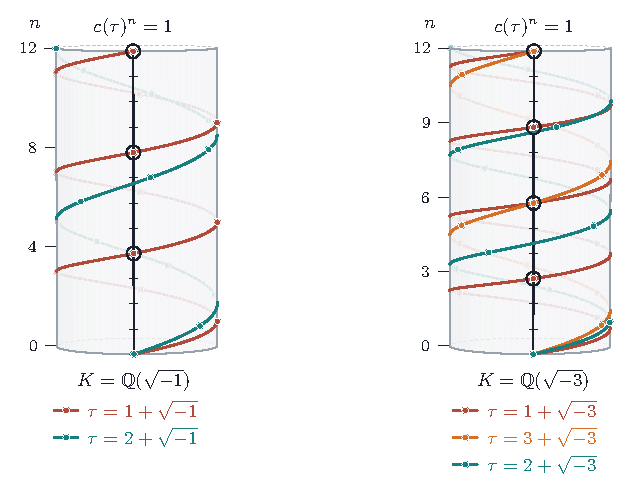
\includegraphics[width=0.78\textwidth]{fig_witness}
\caption{\Cref{rem:witness}. The values $c(\tau)^{n}=(\tau/\bbar\tau)^{n}$,
$0\le n\le12$, on the unit circle, stacked over $n$ as a helix; the
characters $\tau^{2n}$ and $\Nm^{n}$ agree at $\tau$ exactly where the helix
meets the vertical line $c^{n}=1$ (circled). Left, $K=\QQ(\sqrt{-1})$: the
candidate $1+\sqrt{-1}$ returns every fourth step, and $2+\sqrt{-1}$ never.
Right, $K=\QQ(\sqrt{-3})$: $1+\sqrt{-3}$ returns every third step,
$3+\sqrt{-3}$ every sixth, and $2+\sqrt{-3}$ never.}
\label{fig:witness}
\end{figure}

\subsection{The obstruction}

\begin{theorem}[Character obstruction]\label{thm:character}
Let $(A,\iota,\eta)$ be of $(K,-1,n)$-Weil type and write
$H^{1}(A,\QQ)\otimes\CC=V_{+}\oplus V_{-}$ for the decomposition into
eigenspaces of $\iota(\sqrt{-d})$. Then
\[
  H^{2n}(A,\QQ)\otimes\CC
  =\bigoplus_{r+s=2n}\textstyle\bigwedge^{r}V_{+}\otimes\bigwedge^{s}V_{-},
\]
with $\iota(\tau)$ acting on the $(r,s)$ summand by
$\tau^{r}\bbar{\tau}^{\,s}$.
The Weil line $\HW(A)$ spans the two extreme summands $(r,s)=(2n,0)$ and
$(0,2n)$, on which $\Kx$ acts by $\tau^{2n}$ and $\bbar{\tau}^{2n}$, while
$\eta^{n}$ lies in the middle summand $(r,s)=(n,n)$, on which $\Kx$ acts by
the norm character $\Nm_{K/\QQ}(\tau)^{n}$. In particular, for every $n\ge1$,
\[
  \HW(A)\cap H^{2n}(A,\QQ)^{\Nm^{n}}=0,
\]
so a class that is a $\Kx$-eigenclass for $\Nm^{n}$ has zero component along
the Weil line.
\end{theorem}

The theorem shows that the obstruction is structural. A construction that is
equivariant for the $K$-action returns an eigenclass, so it must choose a
character in advance, and the norm character is the one that the
polarisation already occupies. The Weil line sits at the two ends of the
$\Kx$-grading, as far from the middle as the grading allows;
\Cref{fig:charactergrid} draws the grading and marks the two positions.

\begin{proof}[Proof of \Cref{thm:character}]
The grading \eqref{eq:grading} and the action on its summands are given by
\Cref{prop:grading}, the position of $\HW(A)$ by \Cref{lem:weilchar}, and
that of $\eta^{n}$ by \Cref{lem:NSchar}. For the last assertion, write
$H^{2n}(A,\QQ)^{\Nm^{n}}$ for the space of classes $x$ with
$\iota(\tau)^{*}x=\Nm(\tau)^{n}x$ for all $\tau\in\Kx$. After extension of
scalars to $\CC$ this is the isotypic component of the character $\Nm^{n}$,
which by \Cref{prop:grading} is the single summand $(r,s)=(n,n)$. By
\Cref{lem:charsdiffer} the characters $\tau^{2n}$ and $\bbar{\tau}^{\,2n}$
differ from $\Nm^{n}$, so by \Cref{lem:weilchar} the space
$\HW(A)\otimes\CC$ meets the summand $(n,n)$ in zero. Intersecting with
$H^{2n}(A,\QQ)$ gives $\HW(A)\cap H^{2n}(A,\QQ)^{\Nm^{n}}=0$.
\end{proof}

\begin{corollary}[Equivariant classes]%
\label{cor:equivariant}
Let $x\in H^{2n}(A,\QQ)$ satisfy $\iota(\tau)^{*}x=\Nm(\tau)^{n}x$ for all
$\tau\in\Kx$. Then the component of $x$ along $\HW(A)$, with respect to any
$\Kx$-stable complement of $\HW(A)$, is zero. In particular, $x$ is a Weil
class only if $x=0$.
\end{corollary}

\begin{proof}
Let $C$ be a $\Kx$-stable complement of $\HW(A)$ in $H^{2n}(A,\QQ)$ and let
$p$ be the projection onto $\HW(A)$ along $C$. Since both summands are
$\Kx$-stable, $p$ commutes with every $\iota(\tau)^{*}$, so
$\iota(\tau)^{*}p(x)=\Nm(\tau)^{n}p(x)$ for all $\tau\in\Kx$. Hence $p(x)$
lies in $\HW(A)\cap H^{2n}(A,\QQ)^{\Nm^{n}}$, which is zero by
\Cref{thm:character}. If $x$ is a Weil class, then $x=p(x)=0$.
\end{proof}

\Cref{cor:equivariant} is the form of the obstruction that applies to
constructions. A construction that is natural in the $K$-action produces an
eigenclass, whose character is determined by how the input transforms. The
only character available to a rational eigenclass in $H^{2n}(A,\QQ)$ is
$\Nm^{n}$ (\Cref{rem:rightcharacter}). By \Cref{lem:NSchar} this character is
already occupied by the polarisation, and by \Cref{lem:charsdiffer} it is not
a character of the Weil line.

\begin{remark}[Rational eigenclasses]\label{rem:rightcharacter}
To land on the Weil line, a construction must produce classes on which $\Kx$
acts through $\tau\mapsto\tau^{2n}$ or $\tau\mapsto\bbar{\tau}^{\,2n}$, and
neither character is $\QQ$-valued. This rules out rational eigenclasses.
Indeed, let $0\ne x\in H^{k}(A,\QQ)$ satisfy $\iota(\tau)^{*}x=\chi(\tau)\,x$
for all $\tau\in\Kx$. Then $\chi(\tau)\in\QQ$, because $\iota(\tau)^{*}$
preserves $H^{k}(A,\QQ)$. By \Cref{prop:grading}, $x$ lies in a single summand
$(r,s)$ and $\chi(\tau)=\tau^{r}\bbar{\tau}^{\,s}$. Since $\chi$ is
$\QQ$-valued, it equals its conjugate $\tau\mapsto\tau^{s}\bbar{\tau}^{\,r}$,
and the distinctness of the characters in \Cref{prop:grading} gives $r=s$. So
every rational $\Kx$-eigenclass in $H^{2n}(A,\QQ)$ is an eigenclass for
$\Nm^{n}$, and \Cref{cor:equivariant} applies to it. A construction that
reaches the Weil line must therefore produce a class that is not a
$\Kx$-eigenclass. A nonzero element of $\HW(A)$ has nonzero components in both
summands $(2n,0)$ and $(0,2n)$, since complex conjugation interchanges them,
and its $\Kx$-orbit spans the $\QQ$-plane $\HW(A)$. No rational eigenvalue
condition isolates the Weil line: such conditions cut out only the diagonal
summands $(r,r)$, and the Weil line lies at the two ends of the grading.
\end{remark}

\begin{remark}[Determinant and character]\label{rem:failuremode}
A natural chain of statements leads to the opposite conclusion, that $\Kx$
acts on the Weil line through a power of the norm. The Weil line is
$\bigwedge^{2n}_{K}V$, a free $K$-module of rank one; such a module is
two-dimensional over $\QQ$; and multiplication by $\tau$ on it is a
$\QQ$-linear map of determinant $\Nm(\tau)$. Each statement is true, but the
last concerns the $K$-module structure and not the action of $\iota(\tau)$.
By \Cref{lem:weilchar}, $\iota(\tau)$ acts on the Weil line as multiplication
by $\tau^{2n}$, with determinant $\Nm(\tau)^{2n}$, and a space on which $\Kx$
acts through multiplication by $\tau^{2n}$ is not one on which it acts by the
scalar $\Nm(\tau)^{n}$. The first is a $K$-line and the second a
$\QQ$-eigenspace, and they would agree only if $\tau^{n}=\bbar{\tau}^{\,n}$
for all $\tau\in\Kx$, which \Cref{lem:charsdiffer} excludes.
\Cref{fig:charactergrid} draws the distinction.
\end{remark}

\begin{figure}[htbp]
\centering
  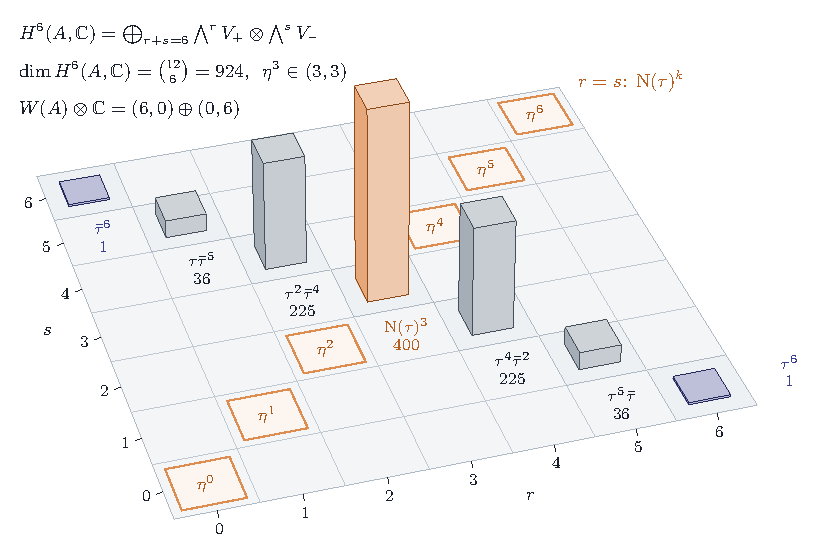
\includegraphics[width=\textwidth]{fig_charactergrid}
\caption{The $\Kx$-grading at $n=3$ on the grid of pairs $(r,s)$,
$0\le r,s\le 6$. The summands $\bigwedge^{r}V_{+}\otimes\bigwedge^{s}V_{-}$ of
$H^{6}(A,\CC)$ lie on the antidiagonal $r+s=6$ and are drawn at their
dimensions $\binom{6}{r}\binom{6}{s}$, which sum to $\binom{12}{6}=924$; on
the summand $(r,s)$ the group $\Kx$ acts by $\tau^{r}\bbar{\tau}^{\,s}$. The
two end cells $(6,0)$ and $(0,6)$, with characters $\tau^{6}$ and
$\bbar{\tau}^{\,6}$, span the Weil line; the middle cell $(3,3)$, with
character $\Nm(\tau)^{3}$, contains $\eta^{3}$. The outlined cells on the
diagonal $r=s$ are the summands on which $\Kx$ acts through a power of the
norm, and they carry the powers $\eta^{k}$. That the end cells and the middle
cell differ is the content of \Cref{thm:character}.}
\label{fig:charactergrid}
\end{figure}

\section{The cohomological Fourier--Mukai transform}\label{sec:fm}

With the character obstruction proved, we turn to the divisor obstruction of
\Cref{thm:divisor}. Its one nontrivial ingredient is a computation: the
cohomological Fourier--Mukai transform sends each power of the polarisation
class to a rational multiple of a power of the polarisation class on the
other side. We prove this in closed form. The computation takes place in a
cohomology ring which, together with the classes involved, depends up to
isomorphism only on the dimension, so one calculation covers every
principally polarised abelian variety at once. Since the Todd class of an
abelian variety is trivial, the passage from sheaves to cohomology is a
formal step.

\subsection{Grothendieck--Riemann--Roch on an abelian variety}

\begin{proposition}\label{prop:grr}
Let $A$ be an abelian variety of dimension $g$ and $\cG$ an object of
$D^{b}(\Av)$. Then
\[
  \ch\bigl(\Phi_{\cP}(\cG)\bigr)=\Phi_{\cP}\bigl(\ch(\cG)\bigr),
\]
where the transform on the right is the cohomological one,
$\Phi_{\cP}(x)=p_{*}\bigl(q^{*}x\cdot\ch(\cP)\bigr)$.
\end{proposition}

\begin{proof}
Grothendieck--Riemann--Roch for the projection
$p\colon A\times\Av\to A$, a proper morphism of smooth varieties, reads
\[
  \ch\bigl(Rp_{*}\cK\bigr)\cdot\td(T_{A})
  =p_{*}\bigl(\ch(\cK)\cdot\td(T_{A\times\Av})\bigr)
\]
for $\cK\in D^{b}(A\times\Av)$. The tangent bundle of an abelian variety is
trivial, so $\td(T_{A})=1$ and $\td(T_{A\times\Av})=1$. Take
$\cK=Lq^{*}\cG\otimes^{L}\cP$, so that $Rp_{*}\cK=\Phi_{\cP}(\cG)$; the
multiplicativity of the Chern character and $\ch(Lq^{*}\cG)=q^{*}\ch(\cG)$
give the statement.
\end{proof}

\subsection{The universal model}

\begin{notation}\label{not:model}
Let $A$ be a principally polarised abelian variety of dimension $g$ with
polarisation class $\theta$, and put $V=H^{1}(A,\QQ)$, a $\QQ$-vector space of
dimension $2g$ carrying the symplectic form attached to $\theta$. Choose a
symplectic basis $e_{1},\dots,e_{2g}$ of $V$ for this form, so that
\begin{equation}\label{eq:thetamodel}
  \theta=\sum_{j=1}^{g}e_{j}\wedge e_{g+j}.
\end{equation}
The principal polarisation identifies $\Av$ with $A$ and
$H^{1}(\Av,\QQ)$ with the dual $V^{\vee}$; let $f_{1},\dots,f_{2g}$ be the
basis dual to $e_{1},\dots,e_{2g}$, so that
\begin{equation}\label{eq:thetapmodel}
  \theta'=\sum_{j=1}^{g}f_{j}\wedge f_{g+j}.
\end{equation}
Then $H^{*}(A\times\Av,\QQ)=\bigwedge^{*}(V\oplus V^{\vee})$.
\end{notation}

\begin{lemma}[The Poincar\'e class]\label{lem:poincare}
In the model of \Cref{not:model},
\begin{equation}\label{eq:ell}
  \ell\coloneqq c_{1}(\cP)=\sum_{i=1}^{2g}e_{i}\wedge f_{i}
  \;\in\;V\otimes V^{\vee}\subset\textstyle\bigwedge^{2}(V\oplus V^{\vee}),
\end{equation}
the canonical element of $V\otimes V^{\vee}=\Hom(V,V)$ corresponding to the
identity, and $\ch(\cP)=e^{\ell}$.
\end{lemma}

\begin{proof}
The Poincar\'e bundle is normalised to be trivial on $A\times\{0\}$ and on
$\{0\}\times\Av$. The components of $c_{1}(\cP)$ in $\bigwedge^{2}V$ and in
$\bigwedge^{2}V^{\vee}$ are its restrictions to these two subvarieties, so
they vanish, and $c_{1}(\cP)$ lies in the middle summand $V\otimes V^{\vee}$
of
$\bigwedge^{2}(V\oplus V^{\vee})=\bigwedge^{2}V\oplus(V\otimes V^{\vee})\oplus\bigwedge^{2}V^{\vee}$.
The defining property of $\cP$ is that its restriction to $A\times\{\lambda\}$
is the line bundle $\lambda$; on cohomology this says that the induced map
$H^{1}(\Av,\QQ)\to H^{1}(A,\QQ)^{\vee}$ obtained by contracting $c_{1}(\cP)$ is
the canonical identification. Equivalently, the element of $\Hom(V,V)$
determined by $c_{1}(\cP)$ is the identity, which is \eqref{eq:ell}. Since
$\cP$ is a line bundle, $\ch(\cP)=e^{c_{1}(\cP)}$.
\end{proof}

\begin{remark}\label{rem:universal}
Every principally polarised abelian variety of dimension $g$ gives, up to
isomorphism, the same data in \Cref{not:model}: a symplectic space of
dimension $2g$ over $\QQ$, its dual, the symplectic form, and the canonical
element. The constants computed
below therefore depend only on $g$ and $k$, and not on $A$.
\end{remark}

\subsection{The closed form}

\begin{theorem}[Transform of the polarisation powers]\label{thm:fmtheta}
Let $A$ be a principally polarised abelian variety of dimension $g$. Then for
every $0\le k\le g$,
\begin{equation}\label{eq:fmtheta}
  \Phi_{\cP}\bigl(\theta'^{\,k}\bigr)
  \;=\;(-1)^{\,g(g+1)/2\,+\,k}\,\frac{k!}{(g-k)!}\;\theta^{\,g-k},
\end{equation}
and $\Phi_{\cP}(\theta'^{\,k})=0$ for $k>g$. In particular
$\Phi_{\cP}\bigl(\QQ[\theta']\bigr)=\QQ[\theta]$.
\end{theorem}

\begin{proof}
Work in the model of \Cref{not:model}. By definition
$\Phi_{\cP}(x)=p_{*}(q^{*}x\cdot e^{\ell})$, and $p_{*}$ extracts the
coefficient of the top exterior form $f_{1}\wedge\cdots\wedge f_{2g}$ in the
$V^{\vee}$ variables: it sends $y\wedge f_{1}\wedge\cdots\wedge f_{2g}$ to
$y$ for $y\in\bigwedge^{*}V$, and kills every class of lower degree in the
$V^{\vee}$ variables.

The classes $e_{i}\wedge f_{i}$ have even degree, so they commute, and they
have square zero. Hence for every $m$,
\begin{equation}\label{eq:ellpower}
  \frac{\ell^{m}}{m!}
  =\sum_{\substack{S\subseteq\{1,\dots,2g\}\\ |S|=m}}\ \prod_{i\in S}e_{i}\wedge f_{i},
\end{equation}
the product being taken in increasing order of $i$. Likewise, from
\eqref{eq:thetapmodel},
\begin{equation}\label{eq:thetappower}
  \frac{\theta'^{\,k}}{k!}
  =\sum_{\substack{T\subseteq\{1,\dots,g\}\\ |T|=k}}\ \prod_{j\in T}f_{j}\wedge f_{g+j},
  \qquad
  \frac{\theta^{\,g-k}}{(g-k)!}
  =\sum_{\substack{U\subseteq\{1,\dots,g\}\\ |U|=g-k}}\ \prod_{j\in U}e_{j}\wedge e_{g+j}.
\end{equation}

Fix $k$. In the product $\theta'^{\,k}\cdot e^{\ell}$, the terms that survive
$p_{*}$ are those of total degree $2g$ in the $f$ variables. A term of
\eqref{eq:thetappower} indexed by $T$ carries the $2k$ variables
$\{f_{j},f_{g+j}:j\in T\}$, and a term of \eqref{eq:ellpower} indexed by $S$
carries the $|S|$ variables $\{f_{i}:i\in S\}$. For the product to be nonzero
the two index sets must be disjoint, and for the total $f$-degree to be $2g$
we need
\[
  S=\{1,\dots,2g\}\setminus\bigl(T\cup(g+T)\bigr),
  \qquad |S|=2g-2k .
\]
So $S$ is determined by $T$, only the term $\ell^{2g-2k}/(2g-2k)!$ of
$e^{\ell}$ contributes, and the surviving terms are in bijection with the
$k$-subsets $T$ of $\{1,\dots,g\}$. Writing $U=\{1,\dots,g\}\setminus T$ we
have $S=U\cup(g+U)$, so the $V$-part of the term indexed by $T$ is
$\prod_{i\in U\cup(g+U)}e_{i}$, which up to sign is the term of
\eqref{eq:thetappower} indexed by $U$. The bijection $T\leftrightarrow U$ is
the one between the terms of $\theta'^{\,k}/k!$ and those of
$\theta^{\,g-k}/(g-k)!$.

It remains to compute the sign $\sigma$ with which each term contributes, and
to check that it is the same for all $T$. The sign is that of the
rearrangement of the ordered word
\[
  \Bigl(\prod_{j\in T}f_{j}f_{g+j}\Bigr)\cdot\Bigl(\prod_{i\in S}e_{i}f_{i}\Bigr)
\]
into the target word
$\bigl(\prod_{j\in U}e_{j}e_{g+j}\bigr)\cdot\bigl(f_{1}\cdots f_{2g}\bigr)$,
which uses the same generators. Relabelling the $g$ symplectic pairs by a
permutation $\pi$ of $\{1,\dots,g\}$ is an automorphism of the exterior
algebra. It
carries the word for $T$ to the word for $\pi(T)$, because the blocks
$f_{j}f_{g+j}$ and $e_{i}f_{i}$ have degree two and may be reordered freely,
and it carries the target word for $U$ to the target word for $\pi(U)$,
because reordering
$f_{\pi(1)}\cdots f_{\pi(g)}f_{g+\pi(1)}\cdots f_{g+\pi(g)}$ costs the
square of the sign of $\pi$. Since the permutations of $\{1,\dots,g\}$ act
transitively on the $k$-subsets, $\sigma=\sigma(g,k)$, and we evaluate it at
$T=\{1,\dots,k\}$. Put $r=g-k$. Moving the $2r$ variables $e_{i}$ of the
second factor to its front costs $(-1)^{r(2r-1)}=(-1)^{r}$, moving them
further past the $2k$ variables of the first factor costs nothing, and
arranging them as $\prod_{j\in U}e_{j}e_{g+j}$ costs $(-1)^{r(r-1)/2}$. The
$f$ variables are left in the order
$f_{1}f_{g+1}\cdots f_{k}f_{g+k}\,f_{k+1}\cdots f_{g}\,f_{g+k+1}\cdots f_{2g}$,
and bringing them to $f_{1}\cdots f_{2g}$ costs $(-1)^{k(k-1)/2+rk}$. As
$r+r(r-1)/2+k(k-1)/2+rk=g(g+1)/2-k$, this gives
\begin{equation}\label{eq:sign}
  \sigma(g,k)=(-1)^{\,g(g+1)/2\,+\,k}.
\end{equation}
Assembling, and accounting for the factorials in \eqref{eq:thetappower},
\[
  \Phi_{\cP}(\theta'^{\,k})
  =k!\cdot\sigma(g,k)\cdot\frac{\theta^{\,g-k}}{(g-k)!},
\]
which is \eqref{eq:fmtheta}. For $k>g$ we have $\theta'^{\,k}=0$, because
$\theta'^{\,k}$ lies in $\bigwedge^{2k}V^{\vee}$, which vanishes for
$2k>2g$. The last assertion follows because the constants in
\eqref{eq:fmtheta} are nonzero for every $0\le k\le g$.
\end{proof}

\begin{remark}[The sign]\label{rem:signcheck}
The sign \eqref{eq:sign} depends only on $g$ and $k$, by the transitivity
argument in the proof, and the count at $T=\{1,\dots,k\}$ fixes it. For even $g=2n$, the case of Weil type,
$g(g+1)/2=n(2n+1)$ has the parity of $n$, and \eqref{eq:sign} reads
$\sigma(2n,k)=(-1)^{n+k}$.
\end{remark}

\begin{corollary}[Stability of the polarisation subring]\label{cor:stability}
Let $A$ be a principally polarised abelian variety and let
$x\in H^{*}(\Av,\QQ)$ lie in the subring $\QQ[\theta']$ generated by $\theta'$.
Then $\Phi_{\cP}(x)\in\QQ[\theta]$.
\end{corollary}

\begin{proof}
The ring $\QQ[\theta']$ is spanned over $\QQ$ by the powers
$\theta'^{\,k}$, \Cref{thm:fmtheta} sends each of them to a rational
multiple of a power of $\theta$, and $\Phi_{\cP}$ is linear.
\end{proof}

\begin{remark}[Non-principal polarisations]\label{rem:nonprincipal}
If $\theta$ is a polarisation of degree $D^{2}$ rather than a principal
one, the isogeny $\phi_{\theta}\colon A\to\Av$ has degree $D^{2}$,
and $\phi_{\theta}^{*}\theta'=D\theta$ for a suitable normalisation of
$\theta'$. The argument of \Cref{thm:fmtheta} goes through with $\theta$
replaced by $D^{-1}\phi_{\theta}^{*}\theta'$, and the constants change
by powers of $D$, all of which are nonzero rationals. The statements below
concern only membership in $\QQ[\theta]$, not the values of the constants, so
we state them for principal polarisations and use them in general.
\end{remark}

\section{The divisor obstruction}\label{sec:divisor}

The first way of reaching a Weil class is to import an object from a
projective space. One restricts an object $\cF$ of $D^{b}(\PP^{N-1})$ to the
dual abelian variety through a morphism $i\colon\Av\to\PP^{N-1}$ and carries
the result back to $A$ by the Fourier--Mukai transform $\Phi_{\cP}$. Secant
varieties of $\Av$ are the usual choice of $\cF$, because a dimension count
makes the codimension come out right, and this is the construction of the
preprint cited on the title page. This section shows that no construction of
this shape produces a Weil class. The proof needs, besides the closed form of
\Cref{sec:fm}, two facts about a morphism to projective space: the Chern
character of a restricted object is a polynomial in the pulled-back
hyperplane class, and this class is the first Chern class of the line bundle
defining the morphism. When the N\'eron--Severi group of $\Av$ has rank one,
the transform therefore lands in $\QQ[\theta]$. We then give two proofs of
\Cref{cor:neverweil}, one through \Cref{prop:notpoly} and one through the
characters of \Cref{sec:characters}, and isolate the equivariance hypothesis
on which the second depends.

\subsection{Statement and proof}

\begin{lemma}[Restriction from an ambient projective space]\label{lem:ambient}
Let $Y$ be a smooth projective variety, let $i\colon Y\to\PP^{N-1}$ be a
morphism defined by a linear system, let $h\in H^{2}(\PP^{N-1},\QQ)$ be the
hyperplane class, and let $\cF\in D^{b}(\PP^{N-1})$. Then
\[
  \ch\bigl(Li^{*}\cF\bigr)\in\QQ\bigl[\,i^{*}h\,\bigr]\subset H^{*}(Y,\QQ).
\]
\end{lemma}

\begin{proof}
The Chern character commutes with derived pullback:
$\ch(Li^{*}\cF)=i^{*}\ch(\cF)$. For a locally free sheaf this follows from
the naturality of Chern classes. It extends to $D^{b}(\PP^{N-1})$ because the
Chern character is additive on distinguished triangles and, by Beilinson's
theorem, every object of $D^{b}(\PP^{N-1})$ is quasi-isomorphic to a finite
complex whose terms are direct sums of line bundles $\cO(-m)$ with
$0\le m\le N-1$. All that is needed is that the classes of line bundles
generate $K_{0}(\PP^{N-1})$, which also follows from the Koszul resolutions
of the structure sheaves of linear subspaces. The cohomology ring of
$\PP^{N-1}$ is $\QQ[h]/(h^{N})$, so $\ch(\cF)$ is a polynomial in $h$ with
rational coefficients, and applying the ring homomorphism $i^{*}$ gives a
polynomial in $i^{*}h$.
\end{proof}

\cite[Remark~2.3]{paperIII} records which other ambient varieties behave in the
same way.

\begin{lemma}[The hyperplane class of a linear system]\label{lem:hyperclass}
Let $A$ be an abelian variety and $i\colon\Av\to\PP^{N-1}$ a morphism defined
by a linear system $|M|$ with $M\in\Pic(\Av)$. Then
$i^{*}h=c_{1}(M)\in\NS(\Av)\otimes\QQ$.
\end{lemma}

\begin{proof}
A morphism to $\PP^{N-1}$ defined by the linear system $|M|$, or by a
subsystem of it, satisfies $i^{*}\cO(1)\cong M$ by construction. Hence
$i^{*}h=c_{1}(i^{*}\cO(1))=c_{1}(M)$.
\end{proof}

\begin{theorem}[Divisor obstruction]\label{thm:divisor}
Let $A$ be a principally polarised complex abelian variety of dimension $g$
with $\NS(\Av)\otimes\QQ=\QQ\cdot\theta'$, let $i\colon\Av\to\PP^{N-1}$ be any
morphism defined by a linear system, and let $\cF$ be any object of
$D^{b}(\PP^{N-1})$. Put $\cE=\Phi_{\cP}(Li^{*}\cF)$. Then
\[
  \ch_{k}(\cE)\in\QQ\cdot\theta^{k}\qquad\text{for every }k\ge0 .
\]
\end{theorem}

\begin{proof}
By \Cref{lem:ambient}, $\ch(Li^{*}\cF)\in\QQ[i^{*}h]$, and by
\Cref{lem:hyperclass}, $i^{*}h=c_{1}(M)$ for the line bundle $M$ defining $i$.
Since $\NS(\Av)\otimes\QQ=\QQ\theta'$, we have $c_{1}(M)=m\theta'$ for some
$m\in\QQ$, and therefore $\ch(Li^{*}\cF)\in\QQ[\theta']$. By
\Cref{prop:grr}, $\ch(\cE)$ is the image of $\ch(Li^{*}\cF)$ under the
cohomological transform $\Phi_{\cP}$, which carries $\QQ[\theta']$ into
$\QQ[\theta]$ by \Cref{cor:stability}. Hence $\ch(\cE)\in\QQ[\theta]$, and
since $\QQ[\theta]\cap H^{2k}(A,\QQ)=\QQ\theta^{k}$, taking the component in
$H^{2k}(A,\QQ)$ gives the statement.
\end{proof}

\begin{remark}[The hypothesis on the N\'eron--Severi group]\label{rem:NShyp}
The hypothesis $\NS(\Av)\otimes\QQ=\QQ\theta'$ holds at the very general point
of any positive-dimensional family of abelian varieties of Weil type with
$\End^{0}(A)=\iota(K)$, which is the case in which the Weil classes lie
outside the divisor subring (\Cref{prop:notpoly}); see \Cref{lem:genericNS}.
Without it, the conclusion is only that $\ch_{k}(\cE)$ lies in the image
under $\Phi_{\cP}$ of the divisor subring of $\Av$. \Cref{thm:character}
makes no hypothesis on $\NS$, which is one reason for giving two proofs of
\Cref{cor:neverweil}.
\end{remark}

\begin{lemma}\label{lem:genericNS}
Let $\mathcal{A}\to S$ be the universal family of abelian varieties of
$(K,-1,n)$-Weil type over the corresponding moduli space, with $n\ge2$. At a
very general point $s\in S$ one has $\End^{0}(A_{s})=\iota(K)$ and
$\NS(A_{s})\otimes\QQ=\QQ\eta_{s}$, of dimension one.
\end{lemma}

\begin{proof}
The locus in $S$ where $\End^{0}$ is strictly larger than $\iota(K)$ is a
countable union of proper closed subvarieties: each additional endomorphism
imposes a nontrivial algebraic condition on the period point, and there are
only countably many candidates, the endomorphisms of the lattice
$H_{1}(A_{s},\ZZ)$. So $\End^{0}(A_{s})=\iota(K)$ at a very general point
$s$, and there the Hodge group is the full special unitary group
$\SU(V,H)$ of the $K$-hermitian form $H$ attached to the
polarisation (\Cref{lem:hermform}), by Weil's computation of the Hodge group of a general abelian
variety of Weil type \cite{Weil77}. The space
$\Hdg^{1}(A_{s})=\NS(A_{s})\otimes\QQ$ is the space of Hodge-group invariants
in $H^{2}(A_{s},\QQ)$. By \Cref{prop:grading} in degree two,
$H^{2}\otimes\CC=\bigwedge^{2}V_{+}\oplus(V_{+}\otimes V_{-})\oplus\bigwedge^{2}V_{-}$.
The group $\SU(V,H)$ acts on $V_{+}\otimes V_{-}\cong V_{+}\otimes V_{+}^{\vee}$
with a one-dimensional space of invariants, spanned by the class of $H$, and on
$\bigwedge^{2}V_{\pm}$ with no invariants, since $2n\ge4$ and $\bigwedge^{2}$
of the standard representation of $\SL_{2n}$ has no invariant vector
unless $2n=2$. Hence the invariants are one-dimensional, and they are spanned
by $\eta_{s}$.
\end{proof}

\subsection{Consequences for Weil classes}

Since a Weil class is by construction not in the subring generated by divisor
classes, the theorem excludes Weil classes at once.

\begin{corollary}\label{cor:neverweil}
With notation as in \Cref{thm:divisor}, suppose in addition that $g=2n$ and
that $(A,\iota,\eta)$ is of $(K,-1,n)$-Weil type. Then $\ch_{n}(\cE)$ is a
Weil class only if $\ch_{n}(\cE)=0$.
\end{corollary}

The first proof passes through \Cref{prop:notpoly}. The second replaces that
proposition by the characters of \Cref{sec:characters} and explains in terms
of representations why the first had to succeed: the $\Kx$-isotypic
decomposition of $H^{2n}(A,\QQ)$ separates the two classes in question
(\Cref{fig:route}).

\begin{proof}[Proof of \Cref{cor:neverweil}]
We work under the hypothesis of \Cref{thm:divisor}. Let $g=2n$ and let
$(A,\iota,\eta)$ be of $(K,-1,n)$-Weil type with
$\NS(A)\otimes\QQ=\QQ\eta$. Then $\theta$ is a nonzero multiple of $\eta$,
and \Cref{thm:divisor} gives
$\ch_{n}(\cE)\in\QQ\cdot\theta^{n}=\QQ\cdot\eta^{n}\subset D^{2n}(A)$. The
proof of \Cref{prop:notpoly} uses the hypothesis $\End^{0}(A)=\iota(K)$ only
to obtain $\NS(A)\otimes\QQ=\QQ\eta$, so it applies here and gives
$\HW(A)\cap D^{2n}(A)=0$. Hence if $\ch_{n}(\cE)$ is a Weil class, it lies in
$\HW(A)\cap D^{2n}(A)=0$.
\end{proof}

\begin{proof}[Second proof of \Cref{cor:neverweil}, via characters]
By \Cref{lem:NSchar} the class $\eta^{n}$ is a $\Kx$-eigenclass for the
character $\Nm^{n}$, and hence so is every nonzero element of $\QQ\eta^{n}$.
As in the first proof, $\ch_{n}(\cE)\in\QQ\eta^{n}$ by
\Cref{thm:divisor}, so $\ch_{n}(\cE)$ satisfies
$\iota(\tau)^{*}\ch_{n}(\cE)=\Nm(\tau)^{n}\ch_{n}(\cE)$ for all $\tau\in\Kx$.
By \Cref{cor:equivariant} it is a Weil class only if it vanishes.
\end{proof}

The second proof uses \Cref{thm:divisor}, and with it the hypothesis on
$\NS$, only to know that $\ch_{n}(\cE)$ is an eigenclass for $\Nm^{n}$; the
rest of the argument uses nothing but this equivariance. We record the
resulting statement, which does not mention the ambient space at all.

\begin{theorem}[Equivariance suffices]\label{thm:equivsuffices}
Let $(A,\iota,\eta)$ be of $(K,-1,n)$-Weil type and let $\cE\in D^{b}(A)$ be
an object such that for every $\tau$ in the order
$\iota^{-1}(\End(A))\subset K$ one has
\[
  \iota(\tau)^{*}\ch_{n}(\cE)=\Nm_{K/\QQ}(\tau)^{n}\,\ch_{n}(\cE).
\]
Then $\ch_{n}(\cE)$ is a Weil class only if $\ch_{n}(\cE)=0$.
\end{theorem}

\begin{proof}
The hypothesis says that $\ch_{n}(\cE)$ is an eigenclass for $\Nm^{n}$ under
the nonzero elements of the order, and it is then one under all of $\Kx$.
Indeed, since the order spans $K$ over $\QQ$, every $\tau\in\Kx$ can be
written as $\sigma/m$ with $\sigma$ in the order and $m$ a nonzero integer.
The endomorphism $\iota(m)$ is multiplication by $m$, which acts on
$H^{2n}(A,\QQ)$ as $m^{2n}=\Nm(m)^{n}$. Hence
$\iota(\tau)^{*}\ch_{n}(\cE)=\Nm(\sigma)^{n}m^{-2n}\ch_{n}(\cE)
=\Nm(\tau)^{n}\ch_{n}(\cE)$, and \Cref{cor:equivariant} applies.
\end{proof}

\begin{remark}[Comparison of the hypotheses]\label{rem:twohyp}
\Cref{thm:divisor} requires the object to be restricted from an ambient
projective space and imposes a condition on $\NS(\Av)$;
\Cref{thm:equivsuffices} requires only that the resulting class be
equivariant for the norm character. The second hypothesis is weaker, and it
holds for any construction whose input is $K$-invariant. This includes the
secant constructions, since the secant varieties of a $K$-invariant
subvariety are $K$-invariant. We state both because the first can be checked
by inspection of the construction, while the second requires an equivariance
computation.
\end{remark}

\begin{figure}[htbp]
\centering
  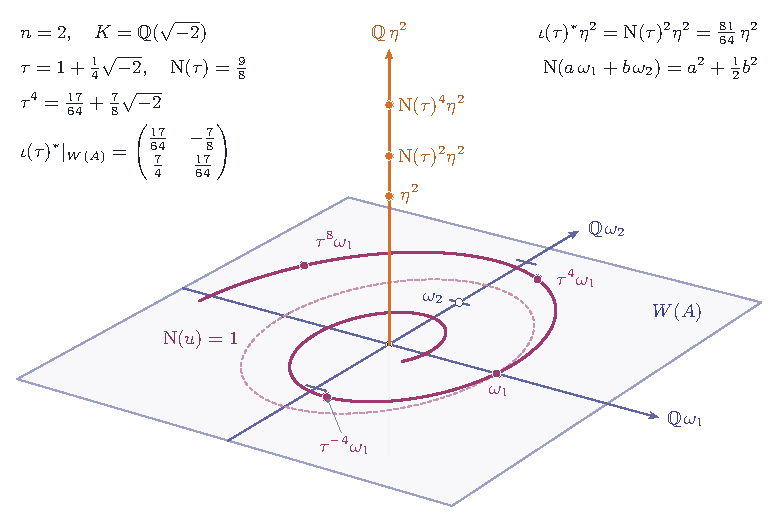
\includegraphics[width=0.96\textwidth]{fig_chernline}
\caption{The linear algebra behind \Cref{thm:divisor}, drawn inside
$H^{2n}(A,\QQ)$. The Weil line $W(A)$ is a plane, free of rank one over $K$
and of rank two over $\QQ$, and $\Kx$ acts on it through $\tau^{2n}$, so the
orbit of any nonzero class is a spiral that spans the plane and lies on no
line in it. The transverse axis carries $\eta^{n}$, on which $\Kx$ acts
through the norm. A construction returning a single eigenclass returns a
line, and by \Cref{prop:orbitplane} no line inside $W(A)$ is stable.}
\label{fig:route}
\end{figure}

\section{Secant numerology}\label{sec:numerology}

The obstructions of \Cref{thm:divisor,thm:character} concern where a class
can lie in cohomology, and neither of them uses a count of dimensions. A
secant construction is also subject to such a count, and this section shows
that the count obstructs nothing. It asks for a polarisation on $\Av$ whose
Euler characteristic lies below the values at which the theorem of Lefschetz
guarantees that a linear system is free of base points or very ample. Those
values are sufficient conditions and not necessary ones, and already on
abelian surfaces there are base-point-free and very ample systems below them.

\subsection{The dimension count}

\begin{setupenv}[The secant numerology]\label{setup:numerology}
Let $A$ be of $(K,-1,n)$-Weil type, so that $\dim A=\dim\Av=2n$. Suppose that
$\Av$ is embedded in $\PP^{N-1}$ by a complete linear system $|M|$ with $M$
ample. An ample line bundle on an abelian variety has no higher cohomology,
so $N=h^{0}(M)=\chi(M)$. The $n$-th secant variety of a nondegenerate
$2n$-fold has expected dimension
\[
  \dim\Sec^{n}(\Av)=n(2n+1)-1=2n^{2}+n-1,
\]
and for a construction that intersects $\Sec^{n}(\Av)$ with $\Av$ in the
expected dimension inside $\PP^{N-1}$,
\[
  \dim\bigl(\Sec^{n}(\Av)\cap\Av\bigr)
  =\bigl(2n^{2}+n-1\bigr)+2n-\bigl(N-1\bigr)
  =2n^{2}+3n-N .
\]
Requiring this dimension to be $n$, so that the construction produces a class
of the required codimension, forces
\begin{equation}\label{eq:chirequired}
  N=\chi(M)=2n^{2}+2n .
\end{equation}
\end{setupenv}

\begin{lemma}\label{lem:chicompare}
For every $n\ge2$,
\[
  2n^{2}+2n<2^{2n}<3^{2n},
\]
and the ratio $2^{2n}/(2n^{2}+2n)$ tends to infinity.
\end{lemma}

\begin{proof}
The right inequality is clear. Since $2^{2n}=4^{n}$, put
$q(n)=4^{n}/(2n^{2}+2n)$, so that $q(2)=16/12>1$. The ratio of consecutive
values is
\[
  \frac{q(n+1)}{q(n)}=\frac{4(2n^{2}+2n)}{2(n+1)^{2}+2(n+1)}=\frac{4n}{n+2},
\]
which is at least $2$ for $n\ge2$. Hence $q(n)\ge2^{\,n-2}q(2)>1$ for every
$n\ge2$, and $q(n)\to\infty$.
\end{proof}

\subsection{The Lefschetz thresholds}

The theorem of Lefschetz says that for $M$ ample on an abelian variety,
$M^{\otimes2}$ is free of base points and $M^{\otimes3}$ is very ample
\cite[Section~4.5]{BL04}. If $M=P^{\otimes2}$ with $P$ ample on an abelian
variety of dimension $m$, then $\chi(M)=2^{m}\chi(P)\ge2^{m}$, since
$\chi(L)=(L^{m})/m!$ for every line bundle $L$ by Riemann--Roch, and similarly
$\chi\ge3^{m}$ in the very ample case. Read as thresholds, these bounds would
say that there is no base-point-free system below $2^{m}$ and no very ample
system below $3^{m}$. Both readings turn a sufficient condition into a
necessary one, and both fail already for abelian surfaces.

\begin{proposition}[The thresholds are not necessary]\label{prop:thresholds}
Let $S$ be a general complex abelian surface, so $m=2$.
\begin{enumerate}[label=\textup{(\roman*)},nosep]
\item A polarisation of type $(1,3)$ on $S$ has $\chi=3<4=2^{2}$ and its
  complete linear system is free of base points; the associated morphism
  $S\to\PP^{2}$ is a six-sheeted covering.
\item A polarisation of type $(1,5)$ on $S$ has $\chi=5<9=3^{2}$ and is very
  ample; the image is a Horrocks--Mumford abelian surface of degree $10$ in
  $\PP^{4}$ \textup{\cite{HM73}}.
\end{enumerate}
In particular neither $2^{m}$ nor $3^{m}$ is a lower bound for the Euler
characteristic of a base-point-free, respectively very ample, ample line
bundle on an abelian variety of dimension $m$.
\end{proposition}

\begin{proof}
By Riemann--Roch on an abelian surface, a polarisation $L$ of type $(1,d)$
has $\chi(L)=(L^{2})/2=d$. The remaining assertions belong to the
classification of $(1,d)$-polarised abelian surfaces; see Gross and Popescu
\cite[\S1.2]{GP98}, where the base locus of $|L|$ is determined for each $d$:
it is empty for $d\ge3$, consists of four points for $d=2$, and $|L|$ is very
ample for $d\ge5$ on a general surface, the case $d=5$ being the
Horrocks--Mumford embedding of \cite{HM73}. In that case the image has degree
$(L^{2})=10$. For $d=3$ the morphism $S\to\PP^{2}$ defined by $|L|$ contracts
no curve, because $L$ is ample, so it is finite and surjective, of degree
$(L^{2})=6$.
\end{proof}

\begin{corollary}\label{cor:nonumerical}
The count of \Cref{setup:numerology} leads to no contradiction. The
requirement $\chi(M)=2n^{2}+2n$ of \eqref{eq:chirequired} is compatible with
$M$ being very ample for all $n$ for which a polarisation of that Euler
characteristic and suitable type exists on a $2n$-dimensional abelian
variety. At $n=2$ the requirement $\chi=12$ on an abelian fourfold is met by
polarisations of type $(1,1,2,6)$ and $(1,1,1,12)$, and nothing in the
numerology excludes very ampleness for either.
\end{corollary}

\begin{remark}[The threshold reading]\label{rem:retract}
The supplementary material of the preprint cited on the title page asserts that the polarisation required by \eqref{eq:chirequired} admits no
base-point-free linear system, on the basis of a table of the values
$2n^{2}+2n$, $2^{2n}$ and $3^{2n}$. The table is correct, and
\Cref{lem:chicompare} reproduces it, but by \Cref{prop:thresholds} the
inference drawn from it does not hold, and the claim is withdrawn. The obstructions of
\Cref{thm:divisor,thm:character} are of a different nature: they bound where
a class can lie in a decomposition of cohomology, and no choice of
polarisation, ambient space or object affects them.
\end{remark}

\section{The semiregularity target}\label{sec:semireg}

Markman's construction at $n=2$ deforms a sheaf across a family and controls
the obstruction by a semiregularity argument in the sense of Bloch and of
Buchweitz and Flenner \cite{Blo72,BF03}. As for the secant construction of
\Cref{sec:numerology}, one may ask whether a dimension count blocks this route
for $n\ge4$. We compute the target of the semiregularity map and show that it
grows too fast for the count to impose any such constraint, so that neither
route meets a numerical obstruction. The constraint that does exist is
structural. In \Cref{ssec:rankzero} we show that the annihilator of the Weil
line in $H^{0,2}(A)$ has dimension $n^{2}$, and that it prevents every object
whose Chern character is concentrated on the Weil line from being
semiregular as soon as $H^{2}(\cO_{A})$ acts on the object faithfully. In
\Cref{ssec:tangent} we identify this annihilator with the tangent space to the
Weil family.

\subsection{The dimension of the target}

\begin{lemma}[Hodge numbers of an abelian variety]\label{lem:hodgenumbers}
For an abelian variety $A$ of dimension $g$ one has
$h^{p,q}(A)=\binom{g}{p}\binom{g}{q}$.
\end{lemma}

\begin{proof}
By \eqref{eq:wedge} and the compatibility of the Hodge decomposition with the
exterior algebra structure,
$H^{p,q}(A)=\bigwedge^{p}H^{1,0}\otimes\bigwedge^{q}H^{0,1}$, and
$\dim H^{1,0}=\dim H^{0,1}=g$.
\end{proof}

\begin{proposition}[The semiregularity target]\label{prop:target}
Let $A$ be an abelian variety of dimension $g=2n$. The target of the
semiregularity map, namely $\bigoplus_{q}H^{q+2}(A,\Omega^{q}_{A})$, has
dimension
\[
  \sum_{q\ge0}h^{q,q+2}(A)=\binom{4n}{2n-2}.
\]
\end{proposition}

\begin{proof}
By \Cref{lem:hodgenumbers} with $g=2n$,
\[
  \sum_{q\ge0}h^{q,q+2}
  =\sum_{q\ge0}\binom{2n}{q}\binom{2n}{q+2}
  =\sum_{q\ge0}\binom{2n}{q}\binom{2n}{2n-q-2}
  =\binom{4n}{2n-2},
\]
the last step being the Vandermonde convolution.
\end{proof}

\begin{corollary}[The dimension count]\label{cor:countnotbind}
The target dimension $\binom{4n}{2n-2}$ takes the values
$28,495,8008,125970,1961256,30421755$ for $n=2,\dots,7$, growing by a factor
exceeding ten at each step. Any source whose dimension grows polynomially in
$n$, for instance the quadratic quantity $\binom{2n}{2}=n(2n-1)$, which takes
the values $6,15,28,45,66,91$ over the same range, is eventually negligible
against it. In particular, for large $n$ a comparison of the two dimensions
cannot obstruct the existence of a semiregular sheaf; the inequality it
produces points the other way.
\end{corollary}

\begin{remark}[Consistency at $n=2$]\label{rem:markmanconsistent}
At $n=2$ the target has dimension $28$, and the sheaf produced by Markman has
$\dim\Ext^{2}=12$, well below it, which is consistent with the construction
succeeding there. Nothing in the numbers changes character between $n=2$ and
$n=4$, so if the construction cannot be carried out for larger $n$, the reason
is not this comparison.
\end{remark}

\begin{remark}[The remaining requirement]\label{rem:semiregneed}
\Cref{cor:countnotbind} does not show that the semiregularity route works.
It removes one apparent obstruction and leaves the actual requirement in
place, namely the construction of a sheaf on $A$ whose Chern character has a
nonzero component along the Weil line. By \Cref{thm:character} such a sheaf
cannot be $K$-equivariant with the norm character, so it cannot be produced
by any functorial construction from $K$-invariant data on $\Av$; Markman's
sheaf at $n=2$ is not produced in this way. In this sense the problem for
$n\ge3$ is one of breaking equivariance, and the dimensions play no role in
it.
\end{remark}

\subsection{The annihilator of the Weil line and objects of rank zero}
\label{ssec:rankzero}

By \Cref{rem:semiregneed}, what remains is to construct a sheaf whose Chern
character has a component along the Weil line. The most economical way to
arrange this is to make the Chern character lie \emph{entirely} on the Weil
line, that is, to take an object of rank zero with every $\ch_{k}$ vanishing
except $\ch_{n}$, as the construction of \Cref{sec:construction} does. We show
that this choice is incompatible with semiregularity whenever $H^{2}(\cO_{A})$
acts faithfully on the object, for a reason that depends only on the position
of the Chern character and not on how the object is built.

We first recall the semiregularity map, on which the rest of this subsection
turns. For a coherent sheaf $\cE$ on a smooth projective variety $A$ the semiregularity
map is defined through the Atiyah class
$\mathrm{At}(\cE)\in\Ext^{1}(\cE,\cE\otimes\Omega^{1}_{A})$: a class
$\xi\in\Ext^{2}(\cE,\cE)$ is sent to the trace of
$\xi\cdot\exp(\mathrm{At}(\cE))$, and the component of that trace in
$H^{q+2}(A,\Omega^{q}_{A})=H^{q,q+2}(A)$ is the $q$-th coordinate of
$\sigma_{\cE}(\xi)$. Bloch introduced the map for local complete
intersections \cite{Blo72}, and Buchweitz and Flenner extended it to
arbitrary coherent sheaves and perfect complexes \cite{BF03}. If $A$ moves in
a family $\cA\to S$, the obstruction to extending $\cE$ to first order along
$v\in T_{s}S$ is a class $\mathrm{ob}_{v}(\cE)\in\Ext^{2}(\cE,\cE)$, and the
theorem of Buchweitz and Flenner identifies $\sigma_{\cE}(\mathrm{ob}_{v}(\cE))$
with the derivative of $\ch(\cE)$ in the direction $v$, projected off the
diagonal of the Hodge decomposition. Hence if $\ch(\cE)$ stays of Hodge type
along $S$, then $\sigma_{\cE}(\mathrm{ob}_{v}(\cE))=0$, and if $\sigma_{\cE}$ is
also injective, then $\mathrm{ob}_{v}(\cE)=0$ and $\cE$ deforms.
Injectivity thus converts a statement about the Chern character into a
statement about the sheaf, and it is the one hypothesis in the argument that
sees more than $\ch(\cE)$.

Two special cases are all that is needed below. For a line bundle $L$ one has
$\Ext^{2}(L,L)=H^{2}(\cO_{A})=H^{0,2}(A)$, and $\sigma_{L}$ is multiplication
by $e^{c_{1}(L)}$. For a direct sum, $\Ext^{2}$ is the sum of the
$\Ext^{2}(\cE_{i},\cE_{j})$, and $\sigma$ acts on each diagonal block
$H^{2}(\cO_{A})\cdot\id_{\cE_{i}}$ by multiplication by the Chern character of
that summand. Both formulae follow at once from the definition by the trace.

\begin{lemma}[The annihilator of the Weil line in $H^{0,2}$]
\label{lem:annihilator}
Let $A$ be of $(K,-1,n)$-Weil type and let $\omega\in\HW(A)\otimes\RR$ be
any nonzero real element of the Weil line. Then the multiplication map
\[
  H^{0,2}(A)\longrightarrow H^{n,n+2}(A),\qquad z\longmapsto z\cdot\omega,
\]
has kernel of dimension exactly $n^{2}$, spanned by the products $u\wedge v$
with $u\in V_{+}^{0,1}$ and $v\in V_{-}^{0,1}$. In particular the kernel is
the same subspace for every $\omega$ on the line.
\end{lemma}

\begin{proof}
Write $\omega=a\,\alpha_{+}+b\,\alpha_{-}$ with $\alpha_{\pm}$ generating
$\bigwedge^{2n}V_{\pm}$, which is possible because
$\HW(A)\otimes\CC=\bigwedge^{2n}V_{+}\oplus\bigwedge^{2n}V_{-}$ (see the proof
of \Cref{prop:weilline}). Complex conjugation interchanges $V_{+}$ and
$V_{-}$, so $\bbar{\alpha}_{+}=\mu\,\alpha_{-}$ for some $\mu\ne0$, and
comparing $\omega$ with $\bbar{\omega}=\omega$ gives $b=\bbar{a}\,\mu$. Since
$\omega\ne0$, the coefficients $a$ and $b$ are therefore both nonzero. As
$H^{0,1}=V_{+}^{0,1}\oplus V_{-}^{0,1}$ with each summand of dimension $n$,
the space $H^{0,2}=\bigwedge^{2}H^{0,1}$ decomposes as
\[
  H^{0,2}
  =\textstyle\bigwedge^{2}V_{+}^{0,1}
  \;\oplus\;\bigl(V_{+}^{0,1}\otimes V_{-}^{0,1}\bigr)
  \;\oplus\;\bigwedge^{2}V_{-}^{0,1},
\]
of dimensions $\binom{n}{2}$, $n^{2}$ and $\binom{n}{2}$.
For $u\in V_{+}^{0,1}$ and $v\in V_{-}^{0,1}$ the mixed product $u\wedge v$
satisfies $u\wedge v\wedge\alpha_{+}=0$, because $u\wedge\alpha_{+}$ lies in
$\bigwedge^{2n+1}V_{+}=0$, and $u\wedge v\wedge\alpha_{-}=0$ for the same
reason with $v$. So the middle summand lies in the kernel.

Conversely, let $z=z_{++}+z_{+-}+z_{--}$ be in the kernel. For the same
reason $z_{++}\wedge\alpha_{+}$, $z_{--}\wedge\alpha_{-}$ and
$z_{+-}\wedge\omega$ vanish, so
$z\cdot\omega=a\,z_{--}\wedge\alpha_{+}+b\,z_{++}\wedge\alpha_{-}$. If $n=1$
the outer summands are zero and there is nothing to prove. If $n\ge2$ the two
terms lie in the distinct summands
$\bigwedge^{2n}V_{+}\otimes\bigwedge^{2}V_{-}$ and
$\bigwedge^{2}V_{+}\otimes\bigwedge^{2n}V_{-}$ of
$\bigwedge^{2n+2}V_{\CC}=\bigwedge^{2n+2}(V_{+}\oplus V_{-})$, so each of them
vanishes. Wedging with a generator of $\bigwedge^{2n}V_{+}$ is injective on
$\bigwedge^{2}V_{-}$, and wedging with a generator of $\bigwedge^{2n}V_{-}$ is
injective on $\bigwedge^{2}V_{+}$. Since $a\neq0$ we get $z_{--}=0$, and since
$b\neq0$ we get $z_{++}=0$, so the kernel is the middle summand.
\end{proof}

The reality of $\omega$ is needed: for the non-real element
$\omega=\alpha_{+}$ of $\HW(A)\otimes\CC$ the same computation gives the
kernel $V_{+}^{0,1}\otimes V_{-}^{0,1}\oplus\bigwedge^{2}V_{+}^{0,1}$, of
dimension $n^{2}+\binom{n}{2}$. \Cref{fig:fibres} draws the mixed block that forms the kernel.

\begin{theorem}[The rank-zero obstruction]
\label{thm:rankzero}
Let $A$ be of $(K,-1,n)$-Weil type. Let $\cE_{1}$ and $\cE_{2}$ be coherent
sheaves on $A$ such that
\[
  \ch(\cE_{1})-\ch(\cE_{2})=c\,\omega,\qquad c\neq0,\quad \omega\in\HW(A),
\]
such that $\Ext^{2}(\cE_{1},\cE_{2})=\Ext^{2}(\cE_{2},\cE_{1})=0$, and such
that the map $H^{2}(\cO_{A})\to\Ext^{2}(\cE_{1},\cE_{1})$,
$z\mapsto z\cdot\id_{\cE_{1}}$, is injective, as it is whenever
$\rk\cE_{1}\neq0$. Put $\cE=\cE_{1}\oplus\cE_{2}$. Then the semiregularity
map
\[
  \sigma_{\cE}\colon\ \Ext^{2}(\cE,\cE)\longrightarrow\bigoplus_{q\ge0}H^{q,q+2}(A)
\]
has kernel of dimension at least $n^{2}$. In particular $\cE$ is not
semiregular, for any $n\ge1$.
\end{theorem}

\begin{proof}
The vanishing of the off-diagonal $\Ext^{2}$ groups gives
$\Ext^{2}(\cE,\cE)=\Ext^{2}(\cE_{1},\cE_{1})\oplus\Ext^{2}(\cE_{2},\cE_{2})$,
and each summand receives $H^{2}(\cO_{A})$ through the $\cO_{A}$-module
structure, $z\mapsto z\cdot\id_{\cE_{i}}$. For $z\in H^{2}(\cO_{A})=H^{0,2}(A)$
consider the element $\xi_{z}=z\cdot\id_{\cE_{1}}-z\cdot\id_{\cE_{2}}$. Its
component in $\Ext^{2}(\cE_{1},\cE_{1})$ is $z\cdot\id_{\cE_{1}}$, so by
hypothesis $z\mapsto\xi_{z}$ is injective. The semiregularity map is
compatible with direct sums, and on $H^{0,2}\cdot\id_{\cE_{i}}$ it is
multiplication by the Chern character of $\cE_{i}$, so
\[
  \sigma_{\cE}(\xi_{z})=z\cdot\ch(\cE_{1})-z\cdot\ch(\cE_{2})
  =c\,z\cdot\omega .
\]
If $\omega=0$ this vanishes for every $z$, and
$\dim H^{0,2}=n(2n-1)\ge n^{2}$. Otherwise $\omega$, being rational, is a
nonzero real element of the Weil line, and by \Cref{lem:annihilator} the
product vanishes for every $z$ in an $n^{2}$-dimensional subspace of
$H^{0,2}$. The corresponding $\xi_{z}$ are linearly independent, and hence
$\dim\ker\sigma_{\cE}\ge n^{2}$.

It remains to justify the claim in the statement that the hypothesis on
$\cE_{1}$ holds in positive rank. For a coherent sheaf $\cF$ the map
$H^{2}(\cO_{A})\to\Ext^{2}(\cF,\cF)$, $z\mapsto z\cdot\id_{\cF}$, is the edge
map of the local-to-global spectral sequence, and
$\operatorname{tr}(z\cdot\id_{\cF})=\rk(\cF)\,z$. When $\rk\cF\ne0$ the trace
therefore splits the map up to the factor $\rk\cF$, and the map is
injective; this applies in particular to a direct sum of line bundles. For a
sheaf of rank zero the map can vanish: for a skyscraper sheaf it factors
through $H^{2}$ of the structure sheaf of a point, which is zero. The direct
sum $\cE_{1}\oplus\cE_{2}$ is used only to produce an element of $\Ext^{2}$
whose image under $\sigma$ is $z\cdot(\ch\cE_{1}-\ch\cE_{2})$ rather than
$z\cdot(\ch\cE_{1}+\ch\cE_{2})$.
\end{proof}

\begin{corollary}[The construction of \Cref{sec:construction}]
\label{cor:pteobstructed}
Let $L_{1},\dots,L_{m}$ be line bundles on $A$ with
$\sum_{i}c_{1}(L_{i})=0$ such that the virtual class
$\sum_{i}\bigl([L_{i}]-[L_{i}^{-1}]\bigr)$ has Chern character on the Weil
line and every difference
$\varepsilon\,c_{1}(L_{i})-\varepsilon'c_{1}(L_{j})$ with
$\varepsilon,\varepsilon'\in\{\pm1\}$ and $(\varepsilon,i)\ne(\varepsilon',j)$
is nondegenerate of index different from $2$. Then the sheaf
$\bigoplus_{i}(L_{i}\oplus L_{i}^{-1})$ has semiregularity kernel of
dimension at least $n^{2}$. At $n=3$ the explicit object of
\Cref{sec:construction} has kernel of dimension exactly
$15=n^{2}+n(n-1)$, of which the $n^{2}=9$ dimensions on the odd side are
the ones supplied by \Cref{thm:rankzero}; the remaining $n(n-1)=6$ come from
the even side and are specific to the line-bundle structure.
\end{corollary}

\begin{proof}
Take $\cE_{1}=\bigoplus L_{i}$ and $\cE_{2}=\bigoplus L_{i}^{-1}$. Then
$\Ext^{2}(\cE_{1},\cE_{2})=\bigoplus_{i,j}H^{2}(L_{i}^{-1}\otimes L_{j}^{-1})$
and $\Ext^{2}(\cE_{2},\cE_{1})=\bigoplus_{i,j}H^{2}(L_{i}\otimes L_{j})$, and
the first Chern classes $\mp\bigl(c_{1}(L_{i})+c_{1}(L_{j})\bigr)$ occurring
here, for all $i$ and $j$, are differences of the kind in the hypothesis,
with $\varepsilon'=-\varepsilon$. A nondegenerate line bundle has cohomology only in
the degree equal to its index, so the index hypothesis gives the required
$\Ext^{2}$ vanishing. The sheaf $\cE_{1}$ has rank $m\ne0$, and the Chern
character hypothesis is that of \Cref{thm:rankzero}.
Since $e^{\lambda}$ and $e^{-\lambda}$ combine into $\cosh\lambda$ and
$\sinh\lambda$, which occupy disjoint degrees, the map splits by parity, and
the odd part is the annihilator of \Cref{lem:annihilator} tensored with the
sign vector. At $n=3$ the dimensions are read off from the proof of
\cite[Proposition~4.14]{paperII}, where the signs are absorbed in the same way:
the kernel consists of the vectors $(u_{i}^{-k}z)_{i}$ with $z$ in the mixed
block $V_{+}^{0,1}\otimes V_{-}^{0,1}$ for $k=3$, which change sign under
$u_{i}\mapsto-u_{i}$, and with $z$ in $\bigwedge^{2}V_{+}^{0,1}$ or
$\bigwedge^{2}V_{-}^{0,1}$ for $k=2$ or $k=4$, which do not.
\end{proof}

\begin{remark}[Uniformity over the configurations]
\label{rem:familyuniform}
By \Cref{cor:pteobstructed} the kernel has dimension at least $n^{2}$ for
every configuration of line bundles $L_{i}^{\pm1}$ whose virtual Chern
character lies on the Weil line and whose differences are nondegenerate of
index different from $2$. The deficiency is therefore not special to the six
line bundles of \cite[Proposition~4.14]{paperII}: \Cref{thm:rankzero} produces it
from the vanishing of the rank alone.

\Cref{thm:rankzero} excludes the economical choice described at the start of
this subsection. An object on which $H^{2}(\cO_{A})$ acts faithfully and which
realises a Weil class through semiregularity cannot have its Chern character
concentrated on the Weil line. It must carry a nonzero rank, or nonzero Chern
character in other degrees, so that $z\mapsto z\cdot\ch(\cE)$ is injective on
$H^{0,2}$; the degree-two component of that product is $\rk(\cE)\cdot z$, and
rank zero is the case in which it vanishes. Markman's sheaves have nonzero
rank, and this is essential to his method: the class he shows to be
deformation-invariant is the normalised character
$\exp(-c_{1}(\cE)/\rk\cE)\ch(\cE)$, which divides by the rank, and the objects
at $n=3$ are reflexive sheaves \cite{Mar25a,Mar25b}. This narrows the fourth
ingredient of \Cref{rem:deformation}: it is a single sheaf of positive rank
whose Chern character has a Weil component alongside other components, rather
than a difference of two sheaves whose classes cancel outside the Weil line.
\end{remark}

\Cref{thm:rankzero} is stated for a direct sum because there the element
$\xi_{z}$ is explicit. The mechanism applies to any perfect complex on which
$H^{2}(\cO_{A})$ acts faithfully, and in particular to the object used in
\Cref{sec:reduction}.

\begin{proposition}[Complexes with concentrated Chern character]
\label{prop:concentrated}
Let $A$ be of $(K,-1,n)$-Weil type and let $E$ be a nonzero perfect complex on
$A$ with $\ch_{k}(E)=0$ for $k\ne n$ and $\ch_{n}(E)=N\omega$ for some
$N\ne0$ and some nonzero $\omega\in\HW(A)$. If the natural map
\begin{equation}\label{eq:idmap}
  H^{2}(\cO_{A})\longrightarrow\Ext^{2}(E,E),\qquad z\longmapsto z\cdot\id_{E},
\end{equation}
is injective, then $\dim\ker\sigma_{E}\ge n^{2}$, so $E$ is not semiregular.
The map \eqref{eq:idmap} is injective whenever $E$ is represented by a virtual
sum of line bundles, in particular at every base point of
\Cref{cor:splitalgebraic}, \Cref{thm:quatweil} and \Cref{thm:everyn}.
\end{proposition}

\begin{proof}
For any perfect complex the semiregularity map satisfies
$\sigma_{E}(z\cdot\id_{E})=z\cdot\ch(E)$, since
$\operatorname{tr}\bigl(z\cdot\id_{E}\circ\exp\mathrm{At}(E)\bigr)
=z\cdot\operatorname{tr}\exp\mathrm{At}(E)=z\cdot\ch(E)$. Hence for $z$ in the
annihilator of $\omega$ in $H^{0,2}(A)$,
\[
  \sigma_{E}(z\cdot\id_{E})=N\,z\cdot\omega=0 ,
\]
and that annihilator has dimension $n^{2}$ by \Cref{lem:annihilator}. If
\eqref{eq:idmap} is injective, the classes $z\cdot\id_{E}$ for $z$ in a basis
of the annihilator are linearly independent, which gives the bound.

For the last sentence, write the class of $E$ in $K_{0}(A)$ as
$\sum_{i}\varepsilon_{i}[L_{i}]$ with $\varepsilon_{i}=\pm1$ and $L_{i}$ line
bundles, and realise it by the direct sum of the $L_{i}$ with
$\varepsilon_{i}=1$ and of the shifts $L_{i}[1]$ of those with
$\varepsilon_{i}=-1$. The map \eqref{eq:idmap} is then $z\mapsto(z,\dots,z)$
into $\bigoplus_{i}\Ext^{2}(L_{i},L_{i})=\bigoplus_{i}H^{2}(\cO_{A})$, which is
injective. At a split member $\omega_{1}$ is a polynomial in
$\beta,\widehat\beta,\ell$ by \Cref{thm:splitclosed}(iii), at a quaternionic
member it is a polynomial in divisor classes by \Cref{thm:quatweil}, and at a
product it is one by \Cref{thm:everyn}; in each case the Chern character is a
ring expression in classes of line bundles, so such a representation exists.
\end{proof}

\begin{proposition}[The class forces the size of the object]%
\label{prop:objectsize}
Let $A$ be of $(K,-1,n)$-Weil type, let $\omega$ be a nonzero element of the
Weil line and let $E$ be a perfect complex on $A$ with
\[
  \ch(E)=r+N\omega,\qquad r\in H^{0}(A,\QQ),\ N\ne0,
\]
and no other component. Then
\[
  \chi(E,E)\;=\;(-1)^{n}N^{2}\!\int_{A}\omega^{2},
\]
independently of $r$, and consequently
\[
  \sum_{i}\dim\Ext^{i}(E,E)\;\ge\;N^{2}\Bigl|\int_{A}\omega^{2}\Bigr|\;>\;0 .
\]
\end{proposition}

\begin{proof}
The Todd class of an abelian variety is $1$, so Riemann--Roch for the Ext
algebra reads $\chi(E,E)=\int_{A}\ch(E)^{\vee}\ch(E)$ with
$\ch_{k}^{\vee}=(-1)^{k}\ch_{k}$. Expanding,
\[
  \ch(E)^{\vee}\ch(E)
  = r^{2}+\bigl(1+(-1)^{n}\bigr)rN\omega+(-1)^{n}N^{2}\omega^{2},
\]
and of the three terms only the last has degree $4n$, so only it survives the
integral; the rank enters solely through $r^{2}$, which sits in degree zero.
For the inequality, $\chi(E,E)=\sum_{i}(-1)^{i}\dim\Ext^{i}(E,E)$, so the
total dimension is at least $|\chi(E,E)|$. Finally $\int_{A}\omega^{2}\ne0$.
Write $\omega=\alpha_{+}+\alpha_{-}$ with $\alpha_{\pm}\in\bigwedge^{2n}V_{\pm}$,
both nonzero by the proof of \Cref{lem:annihilator}. Each $\alpha_{\pm}$ is a
top form on its own eigenspace and squares to zero, so
$\omega^{2}=2\alpha_{+}\alpha_{-}$, which is a nonzero multiple of the
fundamental class.
\end{proof}

\begin{remark}[The constant]\label{rem:sizeconstant}
The bound concerns the whole Ext algebra and does not depend on the rank, so
increasing the rank does not weaken it. The constant $|\int\omega^{2}|$
depends on the normalisation of $\omega$; measured against $\eta$ it picks up
factors of $d$ and of the polarisation type, and no dimension-free growth
rate can be read off from it. The bound uses only that the Weil class is not
isotropic. Together with \Cref{prop:concentrated} it constrains an object
carrying the class in two ways. If the Chern character is concentrated on the
Weil line, the semiregularity map has a kernel of dimension at least $n^{2}$
unless $H^{2}(\cO_{A})$ acts on the object degenerately; and whatever the
rank, the Ext algebra has dimension at least $N^{2}|\int\omega^{2}|$.
\end{remark}

\begin{remark}[Consequences for the semiregularity reduction]
\label{rem:killsreduction}
\cite[Theorem~2.3]{paperII} proves $\Sigma=\cD_{n,n}$, that is, the
algebraicity of the Weil class on the whole family, under the hypothesis that
$\sigma_{E}$ is injective for the complex $E$ of \cite[Proposition~2.1]{paperII}, whose
Chern character is $N\omega_{1}$ in degree $n$ and zero elsewhere. This
complex satisfies the hypotheses of \Cref{prop:concentrated} at every base
point of \Cref{cor:splitalgebraic}, \Cref{thm:quatweil} and
\Cref{thm:everyn}, so there the hypothesis of \cite[Theorem~2.3]{paperII} fails
for it, by $n^{2}$ dimensions.

This does not make \cite[Theorem~2.3]{paperII} vacuous, for two reasons. First,
the hypothesis concerns a chosen perfect complex representing a class in
$K_{0}(A)_{\QQ}$, and distinct representatives of one class have distinct
$\Ext^{2}$ groups; what is ruled out is the representative that the
construction supplies. Second, \Cref{prop:concentrated} needs
\eqref{eq:idmap} to be injective, which is a real restriction for an object
of rank zero: it fails, for instance, for a sheaf supported at a point. A
representative escaping \Cref{prop:concentrated} must therefore
receive $H^{2}(\cO_{A})$ non-injectively, which for a rank-zero object means
that its support is degenerate. Of the two reductions of
\Cref{sec:reduction}, the degree bound of \Cref{thm:degreebound} is untouched
by anything here, and the semiregularity reduction of
\cite[Theorem~2.3]{paperII} is unavailable for the complexes that the
constructions at these base points supply.
\end{remark}

\begin{figure}[t]
\centering
  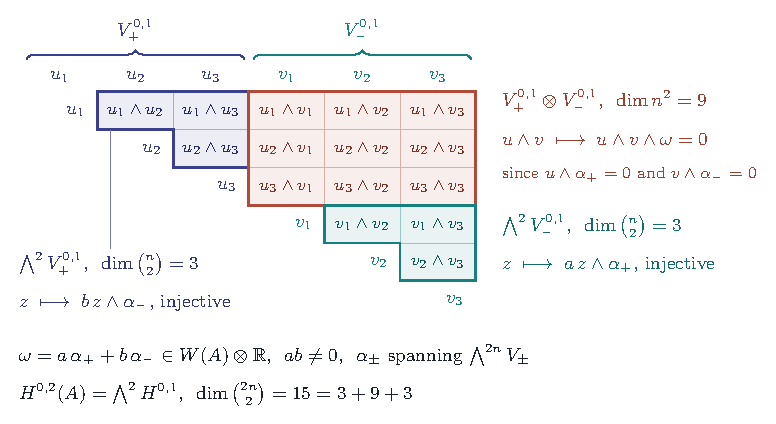
\includegraphics[width=0.94\textwidth]{fig_annihilator}
\caption{The structure behind \Cref{lem:annihilator}, drawn at $n=3$.
$H^{0,2}(A)=\bigwedge^{2}H^{0,1}$ splits into three blocks by how many factors
come from $V_{+}^{0,1}$ and how many from $V_{-}^{0,1}$. The two outer blocks,
of dimension $\binom{n}{2}=3$ each, are carried injectively by multiplication
with the Weil class. The middle block, of dimension $n^{2}=9$ and spanned by
the mixed products, goes to zero, because each such product repeats a factor
of $\alpha_{+}$ and a factor of $\alpha_{-}$. Its dimension $n^{2}$ is the
deficit in \Cref{prop:concentrated}.}
\label{fig:annihilator}
\end{figure}


\subsection{The annihilator and the tangent space to the family}
\label{ssec:tangent}

The number $n^{2}$ of \Cref{lem:annihilator} is also the dimension of the
Weil family. We show in this subsection that the polarisation identifies the
annihilator with the tangent space to the family, canonically and in every
dimension. Two consequences follow. First, the deficiency of the
semiregularity map at an object of rank zero cannot be removed by a better
choice of object, since it is the family itself, seen inside $H^{0,2}$.
Second, the first-order Hodge locus of the Weil line is the Weil family, so
the directions that the semiregularity map cannot see are those along which
the class stays Hodge and along which it would have to be carried.

Write $V_{\pm}$ for the two eigenspaces of $K$ on $H^{1}(A,\CC)$, each of
dimension $2n$, and
\[
  V_{\pm}^{1,0}=V_{\pm}\cap H^{1,0},\qquad
  V_{\pm}^{0,1}=V_{\pm}\cap H^{0,1},
\]
each of dimension $n$ by \Cref{lem:balanced}. Let $E$ denote the
polarisation form on $H^{1}(A,\QQ)$, extended to $H^{1}(A,\CC)$. We use
throughout that $E$ vanishes on $V_{+}\times V_{+}$ and on $V_{-}\times V_{-}$
and pairs $V_{+}$ with $V_{-}$ perfectly, which is condition (iii) of
\Cref{def:weiltype} read on the eigenspaces, and that $E$ vanishes on
$H^{1,0}\times H^{1,0}$ and on $H^{0,1}\times H^{0,1}$, which is the first
Riemann bilinear relation. For the first statement, let $x,y\in V_{+}$. Then
$E(\sqrt{-d}\,x,y)=\sqrt{-d}\,E(x,y)$ from the eigenvalue, and
$E(\sqrt{-d}\,x,y)=-E(x,\sqrt{-d}\,y)=-\sqrt{-d}\,E(x,y)$ from
\Cref{def:weiltype}(iii), so $E(x,y)=0$. The same holds on $V_{-}$, and the
nondegeneracy of $E$ then forces the pairing between $V_{+}$ and $V_{-}$ to
be perfect. Together, the two vanishing statements say that of the four
blocks of $E$ on
$(V_{+}^{1,0}\oplus V_{+}^{0,1})\times(V_{-}^{1,0}\oplus V_{-}^{0,1})$ only
$V_{+}^{1,0}\times V_{-}^{0,1}$ and $V_{+}^{0,1}\times V_{-}^{1,0}$ are
nonzero, and each of these two is a perfect pairing of $n$-dimensional
spaces. This block structure is all that the proof of \Cref{thm:anntangent}
uses of $E$.

A first-order deformation of $A$ is a class in $H^{1}(A,T_{A})$, which for an
abelian variety is canonically $\Hom(H^{1,0},H^{0,1})$, since the tangent
bundle is trivial and $H^{1,0}$ is the dual of its space of sections. Such a
$v$ is extended to $H^{1}(A,\CC)$ by zero on $H^{0,1}$ and acts on
$H^{k}(A,\CC)=\bigwedge^{k}H^{1}(A,\CC)$ as the derivation it generates; we
write $v\lrcorner\,\xi$ for that action. A Hodge class $\xi$ of type $(p,p)$
remains of type $(p,p)$ to first order along $v$ exactly when
$v\lrcorner\,\xi=0$. We call $v$ \emph{polarised} when
$E(vx,y)+E(x,vy)=0$ for all $x,y\in H^{1,0}$, which is the condition that the
deformation preserve the polarisation. The polarised $v$ form a space of
dimension $n(2n+1)=\dim\cA_{2n}$.

\begin{proposition}[The first-order Hodge locus of the Weil line]
\label{prop:firstorder}
Let $A$ be of $(K,-1,n)$-Weil type and let $v$ be a polarised first-order
deformation of $A$. The following are equivalent.
\begin{enumerate}[label=\textup{(\roman*)},nosep]
\item $v\lrcorner\,\omega=0$ for every $\omega$ in the Weil line.
\item $v$ commutes with the action of $K$.
\item $v\bigl(V_{+}^{1,0}\bigr)\subseteq V_{+}^{0,1}$ and
  $v\bigl(V_{-}^{1,0}\bigr)\subseteq V_{-}^{0,1}$.
\end{enumerate}
The space of such $v$ has dimension $n^{2}$, and under
\Cref{prop:weildomain} it is the tangent space at $[A]$ to the Weil family
$\cD_{n,n}$. Each of the two rational generators of the Weil line already
cuts it out by itself.
\end{proposition}

\begin{proof}
The equivalence of (ii) and (iii) is immediate. Since $K$ acts on $V_{\pm}$
by the two scalars $\pm\sqrt{-d}$, commuting with $K$ means preserving $V_{+}$
and $V_{-}$. The extension of $v$ kills $H^{0,1}$ and takes values in
$H^{0,1}$, so preserving $V_{\pm}$ amounts to
$v(V_{\pm}^{1,0})\subseteq V_{\pm}\cap H^{0,1}=V_{\pm}^{0,1}$.

For (i) and (iii), let $\alpha_{+}$ generate $\bigwedge^{2n}V_{+}$ and write
$\alpha_{+}=e_{1}\wedge\cdots\wedge e_{2n}$ for a basis $e_{1},\dots,e_{2n}$
of $V_{+}$ adapted to $V_{+}=V_{+}^{1,0}\oplus V_{+}^{0,1}$. As a derivation,
\[
  v\lrcorner\,\alpha_{+}
  =\sum_{j=1}^{2n}e_{1}\wedge\cdots\wedge v(e_{j})\wedge\cdots\wedge e_{2n}.
\]
Split $v(e_{j})$ along $H^{1}(A,\CC)=V_{+}\oplus V_{-}$. The $V_{+}$
components contribute
$\operatorname{tr}\bigl(\pi_{+}\circ v|_{V_{+}}\bigr)\,\alpha_{+}$, and that
trace vanishes: the map $\pi_{+}\circ v|_{V_{+}}$ kills $V_{+}^{0,1}$ and
carries $V_{+}^{1,0}$ into $V_{+}^{0,1}$, so in the adapted basis its matrix
has zero diagonal blocks. Writing
$v(e_{j})_{-}=\sum_{k}c_{jk}f_{k}$ for a basis $f_{1},\dots,f_{2n}$ of
$V_{-}$, the $V_{-}$ components contribute
\[
  \sum_{j,k}\pm\,c_{jk}\;
  e_{1}\wedge\cdots\wedge\widehat{e_{j}}\wedge\cdots\wedge e_{2n}\wedge f_{k},
\]
and the $4n^{2}$ monomials appearing here are distinct members of the
standard basis of $\bigwedge^{2n}H^{1}(A,\CC)$, hence linearly independent.
So $v\lrcorner\,\alpha_{+}=0$ if and only if every $c_{jk}$ vanishes, which is
$v(V_{+})\subseteq V_{+}$. The same argument on $\alpha_{-}$ gives
$v\lrcorner\,\alpha_{-}=0$ if and only if $v(V_{-})\subseteq V_{-}$. The Weil
line spans $\bigwedge^{2n}V_{+}\oplus\bigwedge^{2n}V_{-}$ over $\CC$ by
\Cref{prop:weilline}, and each of the two rational generators of
\Cref{thm:explicitgens} has both components nonzero, so a single generator
already forces both conditions. This is (i) if and only if (iii).

For the dimension, let $v$ satisfy (iii), and write $v_{+}$ and $v_{-}$ for
its restrictions to $V_{+}^{1,0}$ and $V_{-}^{1,0}$. If $x$ and $y$ both lie
in $V_{+}^{1,0}$, then $v_{+}x$ and $y$ both lie in $V_{+}$, so both terms of
the polarisation condition vanish, and likewise if both lie in $V_{-}^{1,0}$.
For $x\in V_{+}^{1,0}$ and $y\in V_{-}^{1,0}$ the condition reads
$E(v_{+}x,y)=-E(x,v_{-}y)$. The left side is determined by $v_{+}$, and the
pairing between $V_{+}^{1,0}$ and $V_{-}^{0,1}$ is perfect, so for each $y$
there is exactly one $v_{-}y\in V_{-}^{0,1}$ satisfying this for all $x$, and
it depends linearly on $y$. Hence $v_{-}$ is determined by $v_{+}$, which may
be chosen freely, and the polarised deformations satisfying (iii) form a
space of dimension $\dim\Hom(V_{+}^{1,0},V_{+}^{0,1})=n^{2}$. By
\Cref{prop:weildomain} the family $\cD_{n,n}$ is an open subset of the
Grassmannian of $n$-planes in $V_{+}$, whose tangent space at
$V_{+}^{1,0}$ is $\Hom(V_{+}^{1,0},V_{+}/V_{+}^{1,0})=\Hom(V_{+}^{1,0},V_{+}^{0,1})$,
and the identification just made is that isomorphism.
\end{proof}

\begin{proposition}[Infinitesimal rigidity of divisor classes]%
\label{prop:rigidity}
Keep the notation above, put $P=V_{+}^{1,0}$ and $P'=V_{-}^{1,0}$ as in the
proof of \Cref{prop:weildomain}, so that $\bbar{P}=V_{-}^{0,1}$ and
$\bbar{P}'=V_{+}^{0,1}$, and write a class $\delta\in H^{1,1}$ in the four
blocks
\[
  a\ \text{on}\ P\otimes\bbar{P},\quad
  b\ \text{on}\ P'\otimes\bbar{P}',\quad
  c\ \text{on}\ P\otimes\bbar{P}',\quad
  e\ \text{on}\ P'\otimes\bbar{P},
\]
the first two carrying the norm character of $\Kx$ and the last two the
characters $\tau^{2}$ and $\bbar\tau^{\,2}$; reality makes $a$ and $b$
anti-hermitian and ties $e$ to $-\bbar{c}^{\,T}$. Identify the tangent space
$\Hom(P,\bbar{P}')$ to $\cD_{n,n}$ with the $n\times n$ matrices $V$ as in
\Cref{thm:anntangent}, and write $\operatorname{alt}$ for the alternating part
of a matrix, viewed in $\bigwedge^{2}$. Then contraction with a tangent
vector is
\begin{equation}\label{eq:phidelta}
  \Phi_{\delta}(V)
  \;=\;\bigl(\,Va+b^{T}V,\ \ \operatorname{alt}(Vc),\ \
       \operatorname{alt}(-V^{T}e)\,\bigr),
\end{equation}
with values in
$\bbar{P}'\otimes\bbar{P}\oplus\bigwedge^{2}\bbar{P}'\oplus\bigwedge^{2}\bbar{P}
=H^{0,2}$, and $\ker\Phi_{\delta}$ is the tangent space to the locus where
$\delta$ stays of type $(1,1)$. Consequently:
\begin{enumerate}[label=\textup{(\roman*)},nosep]
\item $\Phi_{\delta}=0$ if and only if $\delta$ is a real multiple of $\eta$.
  The rigid classes form a real line, which is the infinitesimal form of the
  statement that $\NS(A)_{\QQ}$ has rank one at the general member.
\item For the norm-character class with block $a$ and $b=c=e=0$,
  \[
    \dim\ker\Phi_{\delta}\;=\;n\,(n-\operatorname{rank}a),
  \]
  so such a class cuts a locus of codimension $n\operatorname{rank}a$, at
  least $n$.
\item A general class has $\ker\Phi_{\delta}=0$: to first order it
  rigidifies the family to a point.
\end{enumerate}
\end{proposition}

\begin{proof}
For \eqref{eq:phidelta}, a polarised deformation commuting with $K$ sends $P$
into $\bbar{P}'$ and $P'$ into $\bbar{P}$, and the polarisation condition
$E(vx,y)+E(x,vy)=0$ forces the second matrix to be $-V^{T}$, as in the proof
of \Cref{prop:firstorder}. Applying $v$ to the $(1,0)$ slot of each block and
collecting terms in $H^{0,2}$ gives the three displayed components; the sign
in the first comes from $\bbar{P}\wedge\bbar{P}'=-\bbar{P}'\wedge\bbar{P}$.

(i) If $\Phi_{\delta}=0$ then $\operatorname{alt}(Vc)=0$ for every $V$, which
for $n\ge2$ forces $c=0$, and likewise $e=0$. The first component gives
$Va=-b^{T}V$ for every $V$; taking $V$ to run over the matrix units shows
$a$ is a scalar $\lambda$ and $b^{T}=-\lambda$. Anti-hermitian scalars are
the purely imaginary ones, so the solutions form a real line. It contains
$\eta$, whose blocks are $a=i$, $b=-i$, and the two therefore agree.

(ii) With $b=c=e=0$ the condition is $Va=0$, that is, the rows of $V$
annihilate the column space of $a$; the solution space has dimension
$n(n-\operatorname{rank}a)$.

(iii) By (ii), the class with $a$ of rank $n$ (for instance $a=i$) and
$b=c=e=0$, which is real since $a$ is anti-hermitian, has
$\ker\Phi_{\delta}=0$. Since $\Phi_{\delta}$ depends linearly on $\delta$, the
classes with $\ker\Phi_{\delta}\ne0$ are cut out by the vanishing of the
maximal minors of $\Phi_{\delta}$ and form a proper real algebraic subset of
the real classes of type $(1,1)$, which gives (iii).
\end{proof}

\begin{remark}[The divisorial supply]\label{rem:rigiditywhy}
\Cref{prop:rigidity}(ii) explains why the divisorial supply of
\Cref{thm:divcriterion} cannot be enlarged by a better choice of class. Any
norm-character class other than a multiple of $\eta$ has
$\operatorname{rank}a\ge1$ and so cuts a locus of codimension at least $n$;
that locus is proper, and by (i) only the real multiples of $\eta$ cut
nothing. Each further class therefore yields a subvariety and never an open
set, which is \Cref{prop:divfails} with the codimension made explicit.
\end{remark}

\begin{figure}[htbp]
\centering
  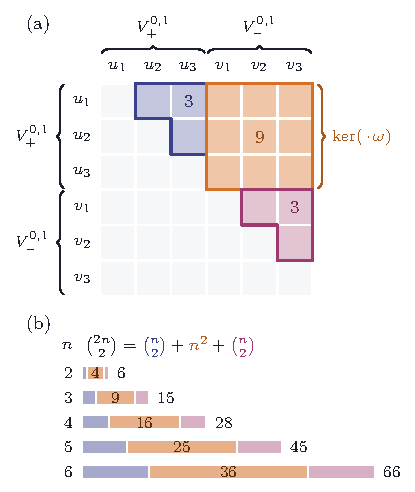
\includegraphics[width=0.46\textwidth]{fig_fibres}
\caption{The geometry behind \Cref{lem:annihilator}, drawn schematically for
the real shadow of the hermitian form. The ruled surface is the null cone of
$H$; the two transverse planes are the conjugate isotropic subspaces $V_{+}$
and $V_{-}$, which conjugation interchanges, so that neither is defined over
$\QQ$ and only their sum is. The segments join a vector of one to its
conjugate in the other, and the strip they sweep stands for the mixed block
$V_{+}^{0,1}\otimes V_{-}^{0,1}$, of dimension $n^{2}$, which multiplication
by the Weil class sends to zero and which is the deficit in
\Cref{prop:concentrated}.}
\label{fig:fibres}
\end{figure}

\begin{theorem}[The annihilator is the tangent space]\label{thm:anntangent}
Let $A$ be of $(K,-1,n)$-Weil type and let $\omega$ be a rational generator of
the Weil line. The polarisation induces an isomorphism
\[
  T_{[A]}\cD_{n,n}\;\xrightarrow{\ \sim\ }\;
  \operatorname{Ann}_{H^{0,2}(A)}(\omega),
\]
canonical in the sense that it depends on no choice of basis and on no choice
of $\omega$ on the line. Explicitly, if $p_{1},\dots,p_{n}$ is a basis of
$V_{+}^{1,0}$ and $q_{1},\dots,q_{n}$ the basis of $V_{-}^{0,1}$ dual to it
under $E$, then $\varphi\in\Hom(V_{+}^{1,0},V_{+}^{0,1})$ corresponds to
\[
  \sum_{a=1}^{n}q_{a}\wedge\varphi(p_{a})\;\in\;
  V_{-}^{0,1}\otimes V_{+}^{0,1}\;\subset\;\textstyle\bigwedge^{2}H^{0,1}
  =H^{0,2}(A).
\]
\end{theorem}

\begin{proof}
The form $E$ pairs $V_{+}$ with $V_{-}$ perfectly and vanishes on
$V_{+}^{1,0}\times V_{-}^{1,0}$, the latter because both spaces lie in
$H^{1,0}$. Hence $E$ restricted to $V_{+}^{1,0}\times V_{-}$ kills
$V_{-}^{1,0}$ and descends to a pairing
\[
  V_{+}^{1,0}\times V_{-}^{0,1}\longrightarrow\CC .
\]
This pairing is perfect: both spaces have dimension $n$, and a vector of
$V_{+}^{1,0}$ orthogonal to $V_{-}^{0,1}$ is orthogonal to all of $V_{-}$,
hence zero. It gives a canonical isomorphism
$\bigl(V_{+}^{1,0}\bigr)^{*}\cong V_{-}^{0,1}$, and therefore
\[
  T_{[A]}\cD_{n,n}
  =\Hom\bigl(V_{+}^{1,0},V_{+}^{0,1}\bigr)
  =\bigl(V_{+}^{1,0}\bigr)^{*}\otimes V_{+}^{0,1}
  \;\cong\;V_{-}^{0,1}\otimes V_{+}^{0,1},
\]
the first equality being the tangent space computation at the end of the proof
of \Cref{prop:firstorder}. Since $H^{0,1}=V_{+}^{0,1}\oplus V_{-}^{0,1}$, the
map $q\otimes u\mapsto q\wedge u$ identifies $V_{-}^{0,1}\otimes V_{+}^{0,1}$
with the middle summand of
$\bigwedge^{2}H^{0,1}$, and that summand is the annihilator by
\Cref{lem:annihilator}. The displayed formula is the composite of these
isomorphisms written in a dual pair of bases, so it is independent of the
basis chosen; and \Cref{lem:annihilator} gives the same subspace for every
$\omega$ on the line, so the isomorphism does not depend on $\omega$ either.
\end{proof}

\begin{figure}[tbp]
\centering
  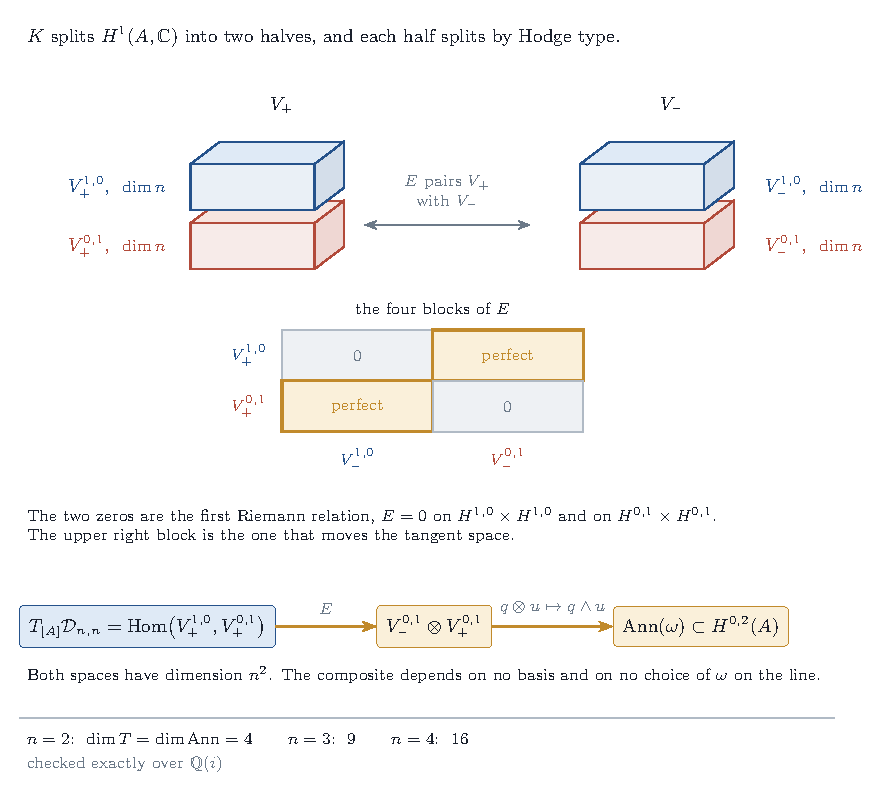
\includegraphics[width=\textwidth]{fig_tangent}
\caption{\Cref{thm:anntangent}. The polarisation has only two nonzero blocks
on $V_{+}\times V_{-}$: it pairs $V_{+}^{1,0}$ with $V_{-}^{0,1}$ and
$V_{+}^{0,1}$ with $V_{-}^{1,0}$, each perfectly, and the other two blocks
vanish by the first Riemann relation. The upper right block turns the tangent
space $\Hom(V_{+}^{1,0},V_{+}^{0,1})$ to the Weil family into
$V_{-}^{0,1}\otimes V_{+}^{0,1}$, which is the middle block of
$\bigwedge^{2}H^{0,1}$ drawn in \Cref{fig:annihilator} and the annihilator of
the Weil line. The two $n^{2}$-dimensional spaces are therefore the same
subspace of $H^{0,2}$, and the directions that the semiregularity map cannot
see are the directions of the family along which the class stays Hodge.}
\label{fig:tangent}
\end{figure}


\begin{corollary}[The kernel contains the tangent space to the family]
\label{cor:kernelfamily}
Let $A$ be of $(K,-1,n)$-Weil type and let $E$ be a nonzero perfect complex on
$A$ satisfying the hypotheses of \Cref{prop:concentrated}, that is, with Chern
character concentrated on the Weil line and with \eqref{eq:idmap} injective.
Then $\ker\sigma_{E}$ contains a subspace canonically isomorphic to
$T_{[A]}\cD_{n,n}$, namely the image of the composite
\[
  T_{[A]}\cD_{n,n}\;\cong\;\operatorname{Ann}_{H^{0,2}}(\omega)
  \;\hookrightarrow\;H^{2}(\cO_{A})\;\xrightarrow{\;z\mapsto z\cdot\id_{E}\;}\;
  \Ext^{2}(E,E).
\]
By \Cref{prop:firstorder} that subspace is also the tangent space to the
first-order Hodge locus of the class $\ch_{n}(E)$.
\end{corollary}

\begin{proof}
Immediate from \Cref{thm:anntangent}, \Cref{prop:concentrated} and
\Cref{prop:firstorder}.
\end{proof}

\begin{theorem}[The weakened criterion is unavailable for concentrated
Chern characters]\label{thm:weakfails}
Let $A$ be of $(K,-1,n)$-Weil type and let $E$ be a nonzero perfect complex on
$A$ satisfying the hypotheses of \Cref{prop:concentrated}. Let
\[
  \operatorname{ev}_{E}\colon HH^{2}(A)\longrightarrow\Ext^{2}(E,E)
\]
be the evaluation on $E$ of the natural transformations $\id\to\id[2]$ of
$D^{b}(A)$, as in \cite[Section 11.4]{Mar25b}. Then
\[
  \operatorname{ev}_{E}\bigl(H^{2}(\cO_{A})\bigr)\cap\ker\sigma_{E}
  =\Delta:=\bigl\{\,z\cdot\id_{E}\;:\;z\in\Ann_{H^{0,2}}(\omega)\,\bigr\},
\]
a subspace of dimension $n^{2}$. In particular $\sigma_{E}$ is not injective
on the image of $\operatorname{ev}_{E}$, so $E$ satisfies neither the
hypothesis of \cite[Lemma 11.3]{Mar25b} nor the weakened hypothesis of
\cite[Question 11.4]{Mar25b}.
\end{theorem}

\begin{proof}
The Hochschild cohomology $HH^{*}(A)=\Ext^{*}_{A\times A}(\cO_{\Delta},\cO_{\Delta})$
is the algebra of natural transformations of the identity functor, and the
Hochschild--Kostant--Rosenberg isomorphism \cite{Cal05,BF08} writes
$HH^{2}(A)\cong H^{2}(\cO_{A})\oplus H^{1}(A,T_{A})\oplus H^{0}(A,\bigwedge^{2}T_{A})$,
with no correction from the Todd class because $T_{A}$ is trivial. The first
summand is the image of $H^{2}(\cO_{A})=\Ext^{2}(\cO_{A},\cO_{A})$ under
pullback to $A\times A$, and the natural transformation it defines sends a
complex $F$ to the composite $F=F\otimes\cO_{A}\xrightarrow{\;\id\otimes z\;}
F\otimes\cO_{A}[2]=F[2]$, that is, to $z\cdot\id_{F}$. This is the statement
that the action of $HH^{*}(A)$ on $\Ext^{*}(F,F)$ restricts on $H^{*}(\cO_{A})$
to the $\cO_{A}$-module structure. Concretely, a class $z\in H^{2}(\cO_{A})$
is represented by a $2$-extension of $\cO_{A}$ by itself; its pullback
$\pi_{1}^{*}z$ to $A\times A$ is a $2$-extension of $\cO_{A\times A}$ by
itself, and tensoring with $\cO_{\Delta}$ gives a $2$-extension of
$\cO_{\Delta}$ by itself, which is the element of $HH^{2}(A)$ in question. The
Fourier--Mukai transform with kernel $\cO_{\Delta}$ is the identity, and the
transform with kernel this extension is the extension of the identity by
itself twisted by $z$, so its value on $F$ is $z\cdot\id_{F}$. Markman uses
this identification when he writes the left vertical arrow of the diagram in
the proof of \cite[Lemma~11.3]{Mar25b} as the HKR isomorphism followed by
contraction with $\ch(E)$. On the summand $H^{2}(\cO_{A})$ contraction is the
cup product $z\mapsto z\cdot\ch(E)$, which is $\sigma_{E}(z\cdot\id_{E})$ by
the computation in the proof of \Cref{thm:rankzero}.

Hence $\operatorname{ev}_{E}(z)=z\cdot\id_{E}$ for $z\in H^{2}(\cO_{A})$, and
$\sigma_{E}(z\cdot\id_{E})=z\cdot\ch(E)=N\,z\cdot\omega$ by the proof of
\Cref{prop:concentrated}, which vanishes exactly for
$z\in\Ann_{H^{0,2}}(\omega)$. So
$\operatorname{ev}_{E}(H^{2}(\cO_{A}))\cap\ker\sigma_{E}=\Delta$, and
$\dim\Delta=\dim\Ann_{H^{0,2}}(\omega)=n^{2}$ by \Cref{lem:annihilator} and
the injectivity of \eqref{eq:idmap}. Since $\Delta\ne0$, the restriction of
$\sigma_{E}$ to the image of $\operatorname{ev}_{E}$ has a nonzero kernel.
The hypothesis of \cite[Lemma 11.3]{Mar25b} is that
$\ker\operatorname{ev}_{E}$ equals the kernel of contraction with $\ch(E)$ and
that $\operatorname{ev}_{E}$ is surjective; the two conditions together would
make $\sigma_{E}$ injective on all of $\Ext^{2}(E,E)$, contradicting
\Cref{prop:concentrated}. The weakened hypothesis of
\cite[Question 11.4]{Mar25b} is injectivity of $\sigma_{E}$ on the image,
which we have just shown to fail.
\end{proof}

\begin{theorem}[A line bundle summand off the polarisation line obstructs]
\label{thm:linebundle}
Let $A$ be of $(K,-1,n)$-Weil type with $n\ge2$ and let $T=T_{[A]}\cD_{n,n}$.
Let $E$ be a perfect complex on $A$ with a direct summand $L[p]$, $L$ a line
bundle, and suppose that $\ch(E)$ remains of Hodge type to first order along
$\cD_{n,n}$, that is $v\lrcorner\,\ch(E)=0$ for every $v\in T$. If $c_{1}(L)$
is not a real multiple of $\eta$, then there is $v\in T$ with
\[
  \operatorname{ev}_{E}(v)\ne0
  \qquad\text{and}\qquad
  \sigma_{E}\bigl(\operatorname{ev}_{E}(v)\bigr)=0 .
\]
Consequently $E$ is not semiregular, does not satisfy the weakened hypothesis
of \cite[Question 11.4]{Mar25b}, and is obstructed to first order along $v$.
The same holds for a twisted complex, with $c_{1}(L)$ replaced by the twisted
first Chern class of the summand, which is $c_{1}(L)$ shifted by the class
common to all summands.
\end{theorem}

\begin{proof}
The class $c_{1}(L)$ is a real class of type $(1,1)$ and not a real multiple
of $\eta$, so by \Cref{prop:rigidity}(i) the contraction
$\Phi_{c_{1}(L)}\colon T\to H^{0,2}(A)$ is not zero: there is $v\in T$ with
$v\lrcorner\,c_{1}(L)\ne0$. On the summand $H^{1}(A,T_{A})$ of $HH^{2}(A)$ the
evaluation map is contraction with the Atiyah class,
$\operatorname{ev}_{E}(v)=v\lrcorner\,\mathrm{At}(E)$. This is the top row of
the diagram of Buchweitz and Flenner reproduced as \cite[(2.1)]{Mar25b}; its
identification with the Hochschild evaluation is in \cite{BF08}, and Markman
uses it in the proof of \cite[Lemma~11.3]{Mar25b}. The Atiyah class of a
direct sum is the direct sum of the Atiyah classes, and that of $L[p]$ is
$c_{1}(L)$, so the
component of $\operatorname{ev}_{E}(v)$ in the summand
$\Ext^{2}(L[p],L[p])=H^{0,2}(A)$ of $\Ext^{2}(E,E)$ is
$v\lrcorner\,c_{1}(L)\ne0$. On the other hand the same diagram gives
$\sigma_{E}(\operatorname{ev}_{E}(v))=v\lrcorner\,\ch(E)$, which vanishes by
hypothesis. So $\operatorname{ev}_{E}(v)$ is a nonzero element of
$\ker\sigma_{E}\cap\image\operatorname{ev}_{E}$; this is the failure of both
hypotheses, and $v\lrcorner\,\mathrm{At}(E)\ne0$ is the statement that $E$
does not lift to a first-order deformation of the pair along $v$, as recalled
in \cite[Section 2]{Mar25b}. Twisting by a class $B$ replaces the Atiyah
class of every rank one summand by its shift by $B$ and $\ch(E)$ by the
twisted Chern character, and nothing else in the argument changes.
\end{proof}

\begin{remark}[Scope of the kernel computation]
\label{rem:whatmeasures}
The semiregularity criterion converts a statement about the Chern character
into a statement about the object by requiring $\sigma_{E}$ to be injective.
\Cref{cor:kernelfamily} says that for an object whose Chern character is
concentrated on the Weil line this requirement fails, and that the failure is
measured by the tangent space to the family across which the class is to be
transported, in every dimension and with no hypothesis beyond
\eqref{eq:idmap}. This concerns the size and the position of the kernel. By
itself it does not say that the obstruction classes are nonzero, nor that
the Weil class fails to deform. For the explicit object of
\cite[Proposition~4.14]{paperII} the obstruction classes are computed in
\cite[Proposition~4.16]{paperII}: they are nonzero in every direction of the
family normal to the split locus, they lie in $\ker\sigma_{E}$, and they meet
the subspace of \Cref{cor:kernelfamily} only in zero. The Weil class deforms
along the family, by \Cref{prop:firstorder}, while that object does not.

The same computation bears on a weaker criterion, which it settles only in
part. Markman asks in \cite[Question 11.4]{Mar25b} whether the
semiregularity theorem survives when $\sigma_{E}$ is required to be injective
only on the image of the evaluation map $\operatorname{ev}_{E}$ rather than
on all of $\Ext^{2}(E,E)$, and records in his Section 12 that an affirmative
answer would carry the method to higher dimensions and to fields of larger
degree. By \Cref{thm:weakfails} the classes of \Cref{cor:kernelfamily} lie in
that image, so for concentrated Chern characters the weakened hypothesis
fails as well, in every dimension and by the same $n^{2}$ dimensions. By
\Cref{thm:linebundle} it fails for every object with a line bundle summand
off the polarisation line, whatever the rank and at every member of the
family, and by \cite[Corollary~4.21]{paperII} this excludes every sum of line bundles.
For the explicit split object of \cite[Proposition~4.14]{paperII} the failure is
complete: \cite[Proposition~4.18]{paperII} shows that every one of the fifteen
dimensions of $\ker\sigma_{E}$ is the value of $\operatorname{ev}_{E}$ on a
Hochschild class that already preserves $\ch(E)$ to first order.

The next question is whether an object of positive rank can satisfy the
weakened hypothesis without satisfying the original one. Markman's own
sheaves are of positive rank and are not of the concentrated shape
(\Cref{rem:familyuniform}); for them he avoids the question by descending to
a quotient on which $\sigma_{E}$ is injective on an invariant subspace
containing the image of $\operatorname{ev}_{E}$
\cite[Proposition~11.5]{Mar25b}. In his Section 12 he proposes a rank one
complex on a principally polarised abelian fourfold, built from $(d+9)/2$
translates of the theta divisor, as a candidate for the weakened criterion in
dimension eight. \cite[Theorem~4.61]{paperII}
shows that the candidate fails, for every discriminant, at every isolated
double point of its support.

Voisin's account of the subject \cite{Voi26} makes the same point
qualitatively, for the variational Hodge conjecture in general: semiregular
objects are hard to construct and too restricted to carry a general argument.
\Cref{cor:kernelfamily} gives this observation a quantitative form for one
family of classes, in which the restriction amounts to $n^{2}$ dimensions and
those dimensions are the tangent directions of the family. Totaro's account
\cite{Tot26} describes Markman's method as the construction of enough
semiregular sheaves to prove the conjecture for abelian fourfolds and
fivefolds, and records that it needed the semiregularity theorem for twisted
sheaves, which Pridham supplied \cite{Pri24}.
\end{remark}


\section{The hyperplane obstruction}\label{sec:hyperplane}

This section sets the constructions on abelian varieties aside and turns to
the other classical approach: induction on the dimension of the variety
through hyperplane sections. One places the variety in a family of hyperplane
sections, uses the algebraicity of the Hodge locus to control where a class
stays of type $(p,p)$, appeals to the conjecture in one dimension lower, and
transports the resulting cycles back up. Each ingredient of such
an argument is a theorem: the Lefschetz hyperplane theorem, hard Lefschetz,
the algebraicity of the Hodge locus \cite{CDK95}, and the properness of
relative Hilbert schemes. The question is whether they compose into an
induction. They do not, for an elementary reason that applies to every
argument of this shape, however the family of hypersurfaces is chosen.

Throughout, $X$ is a smooth complex projective variety of dimension $d$,
$j\colon Y\hookrightarrow X$ is a smooth hypersurface in the linear system of
an ample divisor, and $L=c_{1}(\cO_{X}(Y))\in H^{2}(X,\QQ)$.

\subsection{Two classical inputs}

\begin{theorem}[Lefschetz hyperplane theorem]\label{thm:LHT}
The restriction $j^{*}\colon H^{k}(X,\QQ)\to H^{k}(Y,\QQ)$ is an isomorphism
for $k\le d-2$ and is injective for $k=d-1$.
\end{theorem}

This is the topological form of the theorem. The standard proof, due to
Andreotti and Frankel, is by Morse theory on the smooth affine variety
$X\smallsetminus Y$; see \cite[Chapter~1]{Voi03}.

\begin{lemma}[Gysin and restriction]\label{lem:gysinrestrict}
For every $k$ and every $x\in H^{k}(X,\QQ)$,
\[
  j_{*}j^{*}x=x\cup L .
\]
Moreover $j_{*}\colon H^{k}(Y,\QQ)\to H^{k+2}(X,\QQ)$ is injective for
$k\ge d$.
\end{lemma}

\begin{proof}
The first identity is the projection formula together with
$j_{*}1=[Y]=L$. For the second, Poincar\'e duality on $X$ and on $Y$
identifies $j_{*}\colon H^{k}(Y)\to H^{k+2}(X)$ with the dual of
\[
  j^{*}\colon H^{2d-k-2}(X)\longrightarrow H^{2(d-1)-k}(Y)=H^{2d-k-2}(Y),
\]
so $j_{*}$ is injective on $H^{k}(Y)$ if and only if this $j^{*}$ is
surjective. By \Cref{thm:LHT} that $j^{*}$ is surjective whenever
$2d-k-2\le d-2$, that is whenever $k\ge d$.
\end{proof}

\subsection{The middle degree}

\begin{theorem}[Hyperplane obstruction]\label{thm:hyperplane}
Let $d=2p$ and let $\alpha\in H^{2p}(X,\QQ)$ be primitive. Then
$j^{*}\alpha=0$ for every smooth ample hypersurface $j\colon Y\hookrightarrow X$.
\end{theorem}

The primitive middle degree is where the Hodge conjecture is hard, and it is
where the restriction map returns nothing. \Cref{fig:ladder} draws the
Lefschetz decomposition of an abelian fourfold and the part of it that
restriction annihilates. The proof takes three lines.

\begin{proof}[Proof of \Cref{thm:hyperplane}]
Let $d=2p$ and let $\alpha\in H^{2p}(X,\QQ)$ be primitive. A class of degree
$k\le d$ is primitive when $L^{d-k+1}$ annihilates it, so in the middle degree
primitivity means $L\alpha=0$, that is,
$H^{d}_{\mathrm{prim}}(X,\QQ)=\ker\bigl(L\colon H^{d}(X,\QQ)\to H^{d+2}(X,\QQ)\bigr)$.
By \Cref{lem:gysinrestrict},
\[
  j_{*}\bigl(j^{*}\alpha\bigr)=\alpha\cup L=0 .
\]
The class $j^{*}\alpha$ lies in $H^{d}(Y,\QQ)$, on which $j_{*}$ is injective
by the case $k=d$ of \Cref{lem:gysinrestrict}. Hence $j^{*}\alpha=0$.
\end{proof}

\begin{corollary}[Blindness in the middle degree]\label{cor:blind}
Let $d=2p$ and let $\alpha,\beta\in H^{2p}(X,\QQ)$ be primitive Hodge classes.
Then $j^{*}\alpha=j^{*}\beta=0$ for every smooth ample hypersurface $Y$. In
particular no property of the restricted classes distinguishes $\alpha$ from
$\beta$, and no statement about Hodge classes on hypersurfaces of $X$, however
strong, carries any information about the primitive middle cohomology of $X$.
\end{corollary}

\begin{remark}[The size of what is lost]\label{rem:sizeofloss}
The primitive middle cohomology is not a small correction term. When $X$ is
a smooth hypersurface of degree $m$ in $\PP^{d+1}$, the dimension of
$H^{d}_{\mathrm{prim}}(X,\QQ)$ grows like $m^{d+1}$; and when $d=2p$, the
Hodge conjecture for $X$ in degree $2p$ is the statement that the Hodge
classes in $H^{d}_{\mathrm{prim}}(X,\QQ)$ are algebraic, since the remaining
Hodge classes of degree $2p$ are the multiples of $L^{p}$. By
\Cref{cor:blind}, all of this cohomology is invisible to hyperplane
restriction.
\end{remark}

\subsection{Below the middle degree}

Below the middle degree the restriction map is injective, and in degrees at
most $d-2$ it is an isomorphism, so a class can be transported downwards. The
difficulty moves to the return trip.

\begin{definition}[Lefschetz standard conjecture]\label{def:Bconj}
For a smooth projective variety $X$ of dimension $d$ with ample class $L$,
hard Lefschetz gives isomorphisms
$L^{d-k}\colon H^{k}(X,\QQ)\to H^{2d-k}(X,\QQ)$, and makes $H^{*}(X,\QQ)$
a representation of $\mathfrak{sl}_{2}$ in which $L$ raises the degree by
$2$ and $H$ acts on $H^{k}$ by $k-d$. Let $\Lambda$ denote the unique
endomorphism of degree $-2$ with $[L,\Lambda]=H$. The Lefschetz standard
conjecture $B(X)$ asserts that $\Lambda$ is induced by an algebraic cycle on
$X\times X$; this is equivalent to Kleiman's formulations \cite{Kle68,Kle94}.
\end{definition}

\begin{lemma}[$\Lambda$ undoes $L$ on primitive classes]\label{lem:LambdaL}
Let $\alpha\in H^{k}(X,\QQ)$ be primitive with $k\le d$. Then
$\Lambda L\alpha=(d-k)\,\alpha$.
\end{lemma}

\begin{proof}
This follows from the relation $[L,\Lambda]=H$, where $H$ acts on $H^{k}$ by
the scalar $k-d$, and from $\Lambda\alpha=0$, which holds because the
primitive classes of degree at most $d$ are the lowest weight vectors of the
$\mathfrak{sl}_{2}$-representation. Explicitly,
$\Lambda L\alpha=L\Lambda\alpha-[L,\Lambda]\alpha=0-(k-d)\alpha
=(d-k)\alpha$.
\end{proof}

\begin{theorem}[The return trip]\label{thm:returntrip}
Let $2p\le d-2$, so that $j^{*}\colon H^{2p}(X,\QQ)\to H^{2p}(Y,\QQ)$ is an
isomorphism. If $j^{*}\alpha$ is algebraic on $Y$, then $L\alpha$ is algebraic
on $X$. The implication ``$L\alpha$ algebraic $\Rightarrow$ $\alpha$
algebraic'', asked of all smooth projective $X$ and all Hodge classes
$\alpha$, is
equivalent to the Lefschetz standard conjecture.
\end{theorem}

\begin{proof}[Proof of \Cref{thm:returntrip}]
Let $2p\le d-2$, so $j^{*}\colon H^{2p}(X,\QQ)\to H^{2p}(Y,\QQ)$ is an
isomorphism by \Cref{thm:LHT}. If $j^{*}\alpha=\cl(W)$ for some
$W\in\CH^{p}(Y)_{\QQ}$, then $j_{*}W\in\CH^{p+1}(X)_{\QQ}$ and
\[
  \cl(j_{*}W)=j_{*}j^{*}\alpha=L\alpha
\]
by \Cref{lem:gysinrestrict} and the compatibility of the cycle class map with
proper push-forward, so $L\alpha$ is algebraic.

For the second statement, suppose $B(X)$ holds and $\alpha$ is primitive of
degree $2p<d$ with $L\alpha$ algebraic. Then $\Lambda$ is induced by an algebraic correspondence, hence
carries algebraic classes to algebraic classes, and
$\alpha=(d-2p)^{-1}\Lambda(L\alpha)$ by \Cref{lem:LambdaL}, so $\alpha$ is
algebraic. The same holds without primitivity. Write $P^{m}$ for the
primitive part of $H^{m}(X,\QQ)$. Iterating the relation $[L,\Lambda]=H$ as in
the proof of \Cref{lem:LambdaL} shows that $\Lambda L$ acts on the summand
$L^{i}P^{2p-2i}$ of the Lefschetz decomposition of $H^{2p}(X,\QQ)$ by the
scalar $(i+1)(d-2p+i)$, which is nonzero because $2p<d$. So $\Lambda L$ is
invertible on $H^{2p}(X,\QQ)$, its inverse there is a polynomial in
$\Lambda L$ with rational coefficients, and
$\alpha=(\Lambda L)^{-1}\Lambda(L\alpha)$ is algebraic.

Conversely, suppose that for every smooth projective variety and every Hodge
class $\alpha$ on it the algebraicity of $L\alpha$ implies that of $\alpha$.
Applied repeatedly, this shows that on every smooth projective variety of
dimension $e$ the hard Lefschetz isomorphisms
$L^{e-k}\colon H^{k}\to H^{2e-k}$, $k\le e$, carry the algebraic classes of
degree $k$ onto those of degree $2e-k$, since the preimage of an algebraic
class under $L^{e-k}$ is a Hodge class. This is Kleiman's conjecture $A$ for
every smooth projective variety, and $A$ for $X\times X$ implies $B(X)$
\cite{Kle68,Kle94}.
\end{proof}

Together the two theorems give the following.

\begin{corollary}[No dimensional induction through hyperplane sections]%
\label{cor:noinduction}
Let $X$ be smooth projective of dimension $d$ and let $\alpha\in\Hdg^{p}(X)$.
An argument that deduces the algebraicity of $\alpha$ from the Hodge
conjecture for smooth ample hypersurfaces of $X$, using only $j^{*}$ and
$j_{*}$, returns no information when $2p=d$ and $\alpha$ is primitive, and
otherwise establishes the algebraicity of $L\alpha$ rather than of $\alpha$.
\end{corollary}

\begin{proof}[Proof of \Cref{cor:noinduction}]
Suppose the argument uses only $j^{*}$ and $j_{*}$ to relate classes on $X$ to
classes on smooth ample hypersurfaces $Y\subset X$. First let $2p=d$ with
$\alpha$ primitive. Then $j^{*}\alpha=0$ by \Cref{thm:hyperplane}. A cycle on
$Y$ of codimension $p-1$ has its class in $H^{d-2}(Y,\QQ)$, which is
$j^{*}H^{d-2}(X,\QQ)$ by \Cref{thm:LHT}, so by \Cref{lem:gysinrestrict} its
image under $j_{*}$ lies in $L\cdot H^{d-2}(X,\QQ)$. By the Lefschetz
decomposition this subspace meets the primitive part of $H^{d}(X,\QQ)$ only
in $0$, so $j_{*}$ produces $\alpha$ only when $\alpha=0$, and no conclusion
about $\alpha$ is available. In the remaining cases the best that
$j_{*}j^{*}$ produces is $L\alpha$, and \Cref{thm:returntrip} identifies the
passage from $L\alpha$ to $\alpha$ with the Lefschetz standard conjecture.
\end{proof}

\subsection{Two gaps in inductive arguments}

In practice an induction of this shape breaks at one of two steps, each of
which looks harmless.

\begin{remark}[The dimension bookkeeping]\label{rem:dimensionbookkeeping}
A common formulation places $X$ in a Lefschetz pencil by choosing a generic
pencil $\{X_{t}\}_{t\in\PP^{1}}$ of hyperplane sections \emph{of $X$} and then
setting $X=X_{t_{0}}$ for some $t_{0}$. The two requirements are
incompatible: the members of a pencil of hyperplane sections of $X$ have
dimension $d-1$, so none of them is $X$. An induction that reads
$\dim X_{t}=d-1<d$ in its inductive step, and $X_{t_{0}}=X$ when it transports
the resulting cycle back, is using both readings of the same symbol.

Neither way of resolving the ambiguity rescues the argument. If $X$ is
required to be a member of the pencil, then the pencil lives in an ambient
variety of dimension $d+1$ and every member has dimension $d$; the inductive
parameter does not decrease and the induction is circular. If instead
$\dim X_{t}=d-1$, then the class $\alpha$ lives on $X$ and not on the members,
and the only available transports are $j^{*}$ and $j_{*}$. This is the
situation of \Cref{thm:hyperplane,thm:returntrip}, and \Cref{cor:noinduction}
applies.
\end{remark}

\begin{remark}[Pointwise existence is not a family]\label{rem:pointwise}
The second gap appears in arguments that produce cycles fibrewise and then
assemble them. Suppose an inductive hypothesis furnishes, for each $t$ in the
base $S$ of a family, a cycle $Z_{t}$ with a prescribed class. It does not
follow that the Hilbert polynomial $t\mapsto P_{Z_{t}}$ is constructible, or
semicontinuous, or takes finitely many values. Those are theorems about a flat
family, and the input here is a bare existence statement at each point with
no coherence between points. Without constructibility there is no section of
a relative Hilbert scheme over a dense open subset, and therefore nothing for
the valuative criterion of properness to extend. The step looks safe because
the relative Hilbert scheme of each fixed Hilbert polynomial is proper over
$S$; but properness extends a section that exists over a punctured curve, and
supplies no section where none is given.
\end{remark}

\begin{figure}[htbp]
\centering
  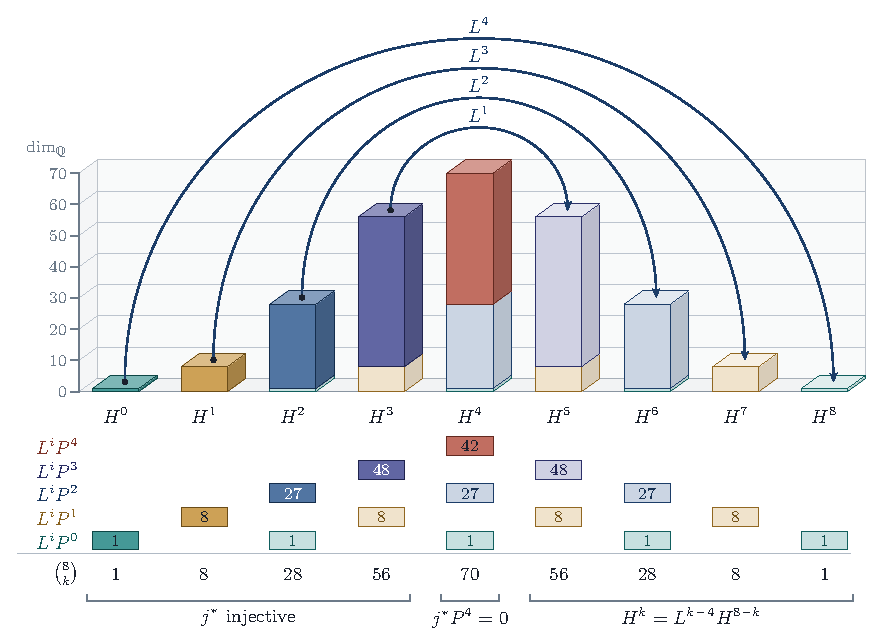
\includegraphics[width=\textwidth]{fig_ladder}
\caption{The Betti numbers $\binom{8}{k}$ of an abelian fourfold, drawn as
prisms and divided according to the Lefschetz decomposition
$H^{k}=\bigoplus_{i}L^{i}P^{k-2i}$: the primitive part $P^{k}$ is drawn dark,
and each image $L^{i}P^{k-2i}$ is drawn light in the colour of $P^{k-2i}$. The
arcs are the hard Lefschetz isomorphisms $L^{4-k}\colon H^{k}\to H^{8-k}$.
Below the middle degree the restriction $j^{*}$ to a smooth ample hypersurface
is injective and a class descends, but the return trip $j_{*}j^{*}$ multiplies
by $L$, and recovering the class is the Lefschetz standard conjecture; above
the middle degree a class is carried to the lower half by an arc. The
primitive middle cohomology $P^{4}$, of dimension $70-28=42$, is annihilated
by $j^{*}$ (\Cref{thm:hyperplane}), and neither an arc nor a restriction
reaches it.}
\label{fig:ladder}
\end{figure}

\section{The Kuga--Satake construction}\label{sec:ks}

\Cref{thm:hyperplane} blocks induction on dimension through hyperplane
sections in the primitive middle degree. One classical construction does reach
a middle degree Hodge class without any such induction, and we set it out in
full, both because it shows what a successful route looks like and because
its boundary is numerical and can be located. It is the construction of Kuga
and Satake \cite{KS67}, which builds on Satake's Clifford algebra families and
their Riemann forms \cite{Sat66}. We follow the form given by Deligne
\cite{Del72}, to whom the Hodge-theoretic properties that make it useful are
due, in particular the embedding of \Cref{prop:ksembed}. After building it we
show that \Cref{thm:hyperplane} has no bearing on it. For abelian varieties of
Weil type with Hodge group $\SU(V,H)$ we then determine when it applies to a
piece of $H^{2}$: exactly when $n=1$, where the Weil line consists of divisor
classes and there is nothing to prove, or $n=2$ with trivial discriminant,
where the Weil line lies in $H^{4}$.

\subsection{The construction}

\begin{setupenv}[K3 type]\label{setup:k3type}
Let $T$ be a $\QQ$-vector space of dimension $b$ with a nondegenerate
symmetric form $q$, and let $T$ carry a Hodge structure of weight two,
$T_{\CC}=T^{2,0}\oplus T^{1,1}\oplus T^{0,2}$, polarised by $q$, with
\[
  \dim_{\CC}T^{2,0}=1 .
\]
Such a structure is said to be \emph{of K3 type}. Write $T^{2,0}=\CC\sigma$.
The Hodge--Riemann relations give $q(\sigma,\sigma)=0$ and
$q(\sigma,\bbar{\sigma})>0$, and make $q$ negative definite on the real points
of $T^{1,1}$; so the real plane
$P=\langle\Re\sigma,\Im\sigma\rangle\subset T_{\RR}$ is positive definite and
$q$ has signature $(2,b-2)$ on $T_{\RR}$. Since $q(\Re\sigma,\Im\sigma)=0$
and $q(\Re\sigma)=q(\Im\sigma)$, we may normalise $\sigma$ so that
$e_{1}=\Re\sigma$ and $e_{2}=\Im\sigma$ are orthonormal.
\end{setupenv}

\begin{definition}[Clifford algebra]\label{def:clifford}
$C(T,q)$ is the quotient of the tensor algebra on $T$ by the ideal generated
by $v\otimes v-q(v)$ for $v\in T$. It is $\ZZ/2$-graded, $C=C^{+}\oplus C^{-}$,
by the parity of the word length.
\end{definition}

\begin{lemma}\label{lem:cliffdim}
For an orthogonal basis $f_{1},\dots,f_{b}$ of $T$ the products $f_{S}$ over
subsets $S\subseteq\{1,\dots,b\}$, taken in increasing order, form a basis of
$C(T,q)$. Hence $\dim_{\QQ}C=2^{b}$ and $\dim_{\QQ}C^{\pm}=2^{b-1}$, and
$C^{-}\cdot C^{+}\cdot C^{-}\subseteq C^{+}$.
\end{lemma}

\begin{proof}
The relations $f_{i}^{2}=q(f_{i})$ and $f_{i}f_{j}=-f_{j}f_{i}$ for $i\ne j$,
the latter obtained by expanding $(f_{i}+f_{j})^{2}=q(f_{i})+q(f_{j})$, let one
rewrite any word in the $f_{i}$ as a scalar times an increasing product, so the
$f_{S}$ span; they are independent by the standard filtration argument
comparing $C$ with $\bigwedge^{*}T$. The dimension counts are
$\sum_{k}\binom{b}{k}=2^{b}$ and
$\sum_{k\ \mathrm{even}}\binom{b}{k}=2^{b-1}$. The last inclusion holds
because the grading is multiplicative and odd plus even plus odd is even.
\end{proof}

\begin{lemma}[The complex structure]\label{lem:cliffJ}
With $e_{1},e_{2}$ as in \Cref{setup:k3type}, put $J=e_{1}e_{2}\in C^{+}\otimes_{\QQ}\RR$.
Then $J^{2}=-1$, and left multiplication by $J$ is an $\RR$-linear operator on
$C^{+}\otimes_{\QQ}\RR$ whose square is $-\id$.
\end{lemma}

\begin{proof}
$J^{2}=e_{1}e_{2}e_{1}e_{2}=-e_{1}e_{1}e_{2}e_{2}=-q(e_{1})q(e_{2})=-1$,
since the orthogonal vectors $e_{1}$ and $e_{2}$ anticommute and
$e_{i}^{2}=q(e_{i})=1$.
Left multiplication by an element of $C^{+}$ preserves $C^{+}$, and the square
of left multiplication by $J$ is left multiplication by $J^{2}=-1$.
\end{proof}

\Cref{fig:ks} draws the positive plane $P$, the null cone of $q$ and the
period domain in the smallest case $b=3$.

\begin{definition}[Kuga--Satake variety]\label{def:ksvariety}
Fix a lattice $C^{+}_{\ZZ}\subset C^{+}$ stable under multiplication. The
complex torus
\[
  \mathrm{KS}(T)=\bigl(C^{+}\otimes_{\QQ}\RR,\,J\bigr)\big/\,C^{+}_{\ZZ}
\]
has dimension $\tfrac12\dim_{\QQ}C^{+}=2^{b-2}$. Satake's construction of a
Riemann form on $C^{+}$ compatible with $J$ \cite{Sat66} makes it an abelian
variety, and by construction
\[
  H^{1}\bigl(\mathrm{KS}(T),\QQ\bigr)=C^{+}(T)
\]
as a Hodge structure of weight one, the Hodge decomposition being the
eigenspace decomposition of left multiplication by $J$.
\end{definition}

\begin{example}\label{ex:ksdims}
For a projective K3 surface, $T$ is the transcendental lattice inside
$H^{2}(X,\QQ)$; taking all of $H^{2}$ with $b=22$ gives
$\dim\mathrm{KS}=2^{20}=1{,}048{,}576$. At the other end, $b=3$ gives
$\dim\mathrm{KS}=2$, an abelian surface, and $b=6$ gives
$\dim\mathrm{KS}=16$; these are the two cases that occur below, for $n=1$ and
for $n=2$.
\end{example}

\subsection{The transport of Hodge classes}

\begin{proposition}[The embedding]\label{prop:ksembed}
Fix $v_{0}\in T$ with $q(v_{0})\ne0$. The map
\[
  \Psi\colon T\longrightarrow\End_{\QQ}\bigl(C^{+}\bigr),
  \qquad
  \Psi(v)(x)=v\,x\,v_{0},
\]
is injective and is a morphism of Hodge structures
$T(1)\to\End\bigl(H^{1}(\mathrm{KS}(T),\QQ)\bigr)$, both sides having weight
zero. Consequently a Hodge class in $T$, that is a rational class of type
$(1,1)$, is carried to a Hodge class of type $(0,0)$ in
$\End(H^{1}(\mathrm{KS}(T),\QQ))$, that is to an element of
$\End^{0}(\mathrm{KS}(T))$.
\end{proposition}

\begin{proof}
The map lands in $\End(C^{+})$ by the last part of \Cref{lem:cliffdim}, since
$v,v_{0}\in T\subset C^{-}$. It is injective because $\Psi(v)(1)=v\,v_{0}$
and $v_{0}$ is invertible in $C(T,q)$, with $v_{0}^{-1}=v_{0}/q(v_{0})$, so
$\Psi(v)=0$ forces $v=0$. That it respects the Hodge structures is
Deligne's computation \cite[\S4]{Del72}: the Hodge structure on
$\End(C^{+})$ is induced by $J$ acting on both sides, and $\Psi$ intertwines
the weight-two structure on $T$, twisted once, with it. The last sentence
follows from the definition of a morphism of Hodge structures and the
Lefschetz theorem on $(1,1)$ classes, in the form which says that for an
abelian variety $B$ a Hodge class of type $(0,0)$ in $\End(H^{1}(B,\QQ))$ is
an element of $\End^{0}(B)$.
\end{proof}

\begin{remark}[Algebraicity of the transport]%
\label{rem:kstransport}
An element of $\End^{0}(\mathrm{KS}(T))$ is a rational multiple of an
endomorphism, whose graph is an algebraic cycle on
$\mathrm{KS}(T)\times\mathrm{KS}(T)$, so the image of a Hodge class under
$\Psi$ is algebraic. Carrying that conclusion back to the variety $X$ from
which $T$ came requires the correspondence $\Psi$ itself to be induced by an
algebraic cycle on $X\times\mathrm{KS}(T)\times\mathrm{KS}(T)$. What is
proved in general is that $\Psi$ is absolute Hodge, by
Deligne's theorem for abelian varieties together with the analysis of the
Kuga--Satake correspondence, and that it is motivated in Andr\'e's sense
\cite{And96}; van Geemen \cite{vG00} surveys the cases in which algebraicity
has been established. The Kuga--Satake construction therefore converts the
Hodge conjecture for $T$ into the algebraicity of one specific
correspondence.
\end{remark}

\subsection{Independence from the hyperplane obstruction}

\begin{proposition}\label{prop:ksnotrestriction}
\Cref{thm:hyperplane,thm:returntrip} do not constrain the Kuga--Satake route.
\end{proposition}

\begin{proof}
Both theorems are statements about the pair of maps $j^{*}$ and $j_{*}$
attached to the inclusion $j\colon Y\hookrightarrow X$ of a smooth member of an
ample linear system, and both proofs use two properties of that pair which a
general correspondence does not have: the Lefschetz hyperplane theorem, which
makes $j^{*}$ an isomorphism in degrees at most $d-2$ and, through
\Cref{lem:gysinrestrict}, forces the vanishing of \Cref{thm:hyperplane} in
the primitive middle degree; and the identity $j_{*}j^{*}=\,\cdot\cup L$ of
\Cref{lem:gysinrestrict}, which makes the return trip multiply by the
polarisation instead of recovering the class. The Kuga--Satake
correspondence is a cohomology class on a triple product of varieties of
unrelated dimensions, $\dim\mathrm{KS}(T)=2^{b-2}$ against $\dim X$, and it has
neither property; in particular the composite of $\Psi$ with its transpose is
a nonzero multiple of the identity of $T$, not a power of a polarisation of
$X$. So
neither of the two properties on which \Cref{thm:hyperplane} rests holds for
$\Psi$.
\end{proof}

\Cref{prop:ksnotrestriction} shows what an escape from \Cref{thm:hyperplane}
must look like: a correspondence whose composite with its transpose is not the
Lefschetz operator. \Cref{sec:escape} makes the analogous identification for
\Cref{thm:divisor,thm:character}.

\subsection{Abelian varieties of Weil type}

The limitation of the Kuga--Satake construction is the hypothesis
$\dim T^{2,0}=1$. For abelian varieties of Weil type the rational sub-Hodge
structures of $H^{2}$, and hence the possible values of $\dim T^{2,0}$, can be
listed completely.

\begin{proposition}[The pieces of \texorpdfstring{$H^{2}$}{H2}]\label{prop:h2pieces}
Let $(A,\iota,\eta)$ be of $(K,-1,n)$-Weil type. In the character grading of
\Cref{prop:grading},
\begin{equation}\label{eq:h2split}
  H^{2}(A,\CC)
  =\textstyle\bigwedge^{2}V_{+}\;\oplus\;\bigl(V_{+}\otimes V_{-}\bigr)
   \;\oplus\;\bigwedge^{2}V_{-},
\end{equation}
the middle summand is the isotypic component of the norm character and is
defined over $\QQ$, and the outer two are interchanged by conjugation so their
sum is defined over $\QQ$. The Hodge numbers are
\[
  \bigl(h^{2,0},h^{1,1},h^{0,2}\bigr)=
  \begin{cases}
    \bigl(\tbinom{n}{2},\,n^{2},\,\tbinom{n}{2}\bigr)
      & \text{on }\bigwedge^{2}V_{\pm},\\[4pt]
    \bigl(n^{2},\,2n^{2},\,n^{2}\bigr)
      & \text{on }V_{+}\otimes V_{-},
  \end{cases}
\]
and the total is $2\tbinom{2n}{2}+4n^{2}=\tbinom{4n}{2}=\dim H^{2}(A,\QQ)$.
\end{proposition}

\begin{proof}
The splitting is \eqref{eq:grading} at $k=2$. The characters are
$\tau^{2}$, $\tau\bbar{\tau}=\Nm(\tau)$ and $\bbar{\tau}^{2}$, so the middle
summand is the norm-isotypic component, and it is self-conjugate, hence defined
over $\QQ$; the outer two are exchanged. For the Hodge numbers use
\eqref{eq:bisplit} and \Cref{lem:balanced}: $V_{\pm}^{1,0}$ and
$V_{\pm}^{0,1}$ have dimension $n$ each, so
$(\bigwedge^{2}V_{+})^{2,0}=\bigwedge^{2}V^{1,0}_{+}$ has dimension
$\binom{n}{2}$ and $(\bigwedge^{2}V_{+})^{1,1}=V^{1,0}_{+}\otimes V^{0,1}_{+}$
has dimension $n^{2}$, while
$(V_{+}\otimes V_{-})^{2,0}=V^{1,0}_{+}\otimes V^{1,0}_{-}$ has dimension
$n^{2}$ and the $(1,1)$ part has dimension $2n^{2}$. The total is
$2(2\binom{n}{2}+n^{2})+4n^{2}=2(2n^{2}-n)+4n^{2}=8n^{2}-2n=\binom{4n}{2}$.
\end{proof}

\begin{proposition}[Sub-Hodge structures of K3 type]%
\label{prop:normpart}
Let $(A,\iota,\eta)$ be of $(K,-1,n)$-Weil type with $\Hg(A)=\SU(V,H)$. Then
$H^{2}(A,\QQ)$ is the direct sum of the three rational sub-Hodge structures
\[
  \QQ\,\eta,
  \qquad
  \bigl(V_{+}\otimes V_{-}\bigr)_{\QQ}\ominus\QQ\eta,
  \qquad
  R=\Bigl(\textstyle\bigwedge^{2}V_{+}\oplus\bigwedge^{2}V_{-}\Bigr)_{\QQ},
\]
with $h^{2,0}$ equal to $0$, $n^{2}$ and $n(n-1)$ respectively. The first two
are irreducible, and so is $R$ when $n\ge3$. When $n=2$, the structure $R$ is
irreducible if the discriminant of $(A,\iota,\eta)$ in the sense of
\Cref{def:disc} is nontrivial, and it is the direct sum of two isomorphic
sub-Hodge structures of K3 type, each of dimension six, if the discriminant
is trivial. Consequently $H^{2}(A,\QQ)$ contains a rational sub-Hodge
structure of K3 type if and only if either $n=1$, or $n=2$ and the
discriminant is trivial.
\end{proposition}

\begin{proof}
A rational sub-Hodge structure $W\subseteq H^{2}(A,\QQ)$ is stable under
$\Hg(A)$: the orthogonal projector onto $W$ for the polarisation is a Hodge
class in $\End(H^{2})$, hence is fixed by $\Hg(A)$, hence $W$ is a
$\Hg(A)$-submodule. Conversely a $\Hg(A)$-submodule is a sub-Hodge structure,
because the Hodge decomposition is the eigenspace decomposition of an element
of $\Hg(A)(\RR)$. So the rational sub-Hodge structures are the
$\QQ$-subrepresentations of $\SU(V,H)$. For the same reason the Hodge numbers
of a sub-Hodge structure depend only on its complexification as a
representation of $\Hg(A)_{\CC}$.

After complexification $\SU(V,H)$ becomes $\SL(V_{+})$, acting on $V_{+}$
tautologically and on $V_{-}\cong V_{+}^{\vee}$ dually. In \eqref{eq:h2split}
the outer summands $\bigwedge^{2}V_{+}$ and
$\bigwedge^{2}V_{-}\cong\bigwedge^{2}V_{+}^{\vee}$ are irreducible, and the
middle summand is $V_{+}\otimes V_{+}^{\vee}=\End(V_{+})
=\mathfrak{sl}(V_{+})\oplus\CC$, the sum of the adjoint representation and the
trivial one. Conjugation fixes the two pieces of the middle summand and
exchanges the outer two, so the three listed subspaces are rational sub-Hodge
structures, and the first two, having irreducible complexifications, are
irreducible. The trivial summand is spanned by $\eta$ by \Cref{lem:NSchar},
and has $h^{2,0}=0$ since $\eta$ is of type $(1,1)$. The adjoint summand has
$h^{2,0}=n^{2}$, since removing the one-dimensional trivial piece from
$V_{+}\otimes V_{-}$ removes a $(1,1)$ class only. The structure $R$ has
$h^{2,0}=2\binom{n}{2}=n(n-1)$ by \Cref{prop:h2pieces}.

The complexification of a rational subrepresentation of $R$ is a
subrepresentation of $\bigwedge^{2}V_{+}\oplus\bigwedge^{2}V_{-}$ stable under
conjugation. For $n\ge3$ the two summands are not isomorphic, because
$\bigwedge^{2}V_{+}^{\vee}\cong\bigwedge^{2n-2}V_{+}$ and $2n-2\ne2$. The
subrepresentations are then $0$, the two summands and the whole; conjugation
exchanges the summands, so only $0$ and the whole are stable under it, and
$R$ is irreducible.
For $n=1$ both summands are the trivial representation, and $R$ is the plane
of Hodge classes $\HW(A)\subset H^{2}(A,\QQ)$.

Let $n=2$. Then $\bigwedge^{2}V_{+}^{\vee}\cong\bigwedge^{2}V_{+}\otimes
(\bigwedge^{4}V_{+})^{\vee}\cong\bigwedge^{2}V_{+}$ as representations of
$\SL(V_{+})$, so $\End_{\Hg(A)}(R)\otimes\CC\cong M_{2}(\CC)$ and
$\End_{\Hg(A)}(R)$ is a quaternion algebra over $\QQ$. To identify it, put
$V=H^{1}(A,\QQ)$, a $K$-vector space of dimension four by \Cref{lem:Kspace}.
The natural map $\bigwedge^{2}_{\QQ}V\to\bigwedge^{2}_{K}V$ is
$\SU(V,H)$-equivariant, and its kernel has complexification
$V_{+}\otimes V_{-}$, so it restricts to an isomorphism of $R$ onto
$\bigwedge^{2}_{K}V$; in particular $K\subseteq\End_{\Hg(A)}(R)$. The wedge
product $B\colon\bigwedge^{2}_{K}V\times\bigwedge^{2}_{K}V\to
\bigwedge^{4}_{K}V\cong K$ is a symmetric $K$-bilinear form, invariant under
$\SU(V,H)$ because $\SU(V,H)$ acts trivially on $\bigwedge^{4}_{K}V$. Let
$H_{2}$ be the hermitian form induced by $H$ on $\bigwedge^{2}_{K}V$, and let
$\varphi$ be the $K$-antilinear map defined by
$B(x,y)=H_{2}\bigl(y,\varphi(x)\bigr)$. Then $\varphi$ commutes with
$\SU(V,H)$, so $\varphi^{2}$ is a $K$-linear endomorphism commuting with
$\SU(V,H)$; it is a scalar by Schur's lemma, and a rational one because it
commutes with $\varphi$. Choose a $K$-basis $e_{1},\dots,e_{4}$ of $V$
orthogonal for $H$, with $H(e_{i},e_{i})=h_{i}\in\QQ^{\times}$, and identify
$\bigwedge^{4}_{K}V$ with $K$ through $e_{1}\wedge e_{2}\wedge e_{3}\wedge
e_{4}$. Then $\varphi(e_{1}\wedge e_{2})=(h_{3}h_{4})^{-1}e_{3}\wedge e_{4}$
and $\varphi(e_{3}\wedge e_{4})=(h_{1}h_{2})^{-1}e_{1}\wedge e_{2}$, so
$\varphi^{2}=(\det H)^{-1}$. Hence $\End_{\Hg(A)}(R)=K\oplus K\varphi$ is the
quaternion algebra $(-d,\det H)_{\QQ}$. It is split if and only if
$\det H\in\Nm_{K/\QQ}(\Kx)$, that is, since $(-1)^{2}\det H=\det H$, if and
only if the discriminant is trivial. If it is not split it is a division
algebra, and $R$ is irreducible. If it is split, $R=R_{1}\oplus R_{2}$ with
$R_{1}\cong R_{2}$ of dimension six, and the complexification of each $R_{i}$
is isomorphic to $\bigwedge^{2}V_{+}$ as a representation of $\SL(V_{+})$, so
by \Cref{prop:h2pieces} each $R_{i}$ has Hodge numbers $(1,4,1)$. Each $R_{i}$
lies in the primitive part of $H^{2}(A,\QQ)$, which is the $\Hg(A)$-stable
complement of $\QQ\eta$, and is polarised by the restriction of the
Hodge--Riemann form; so $R_{i}$ is of K3 type.

Finally, a rational sub-Hodge structure of $H^{2}(A,\QQ)$ is a direct sum of
irreducible ones, each isomorphic to $\QQ\eta$, to the adjoint structure, to
$R$, or, for $n=2$ and trivial discriminant, to $R_{1}$; and $h^{2,0}$ is
additive. A structure of K3 type has $h^{2,0}=1$. For $n=1$ the adjoint
structure has $h^{2,0}=1$. For $n\ge3$ the nonzero values $n^{2}$ and
$n(n-1)$ both exceed $1$. For $n=2$ the values are $0$, $4$, and $2$ for $R$
or $1$ for $R_{1}$, so a structure of K3 type exists if and only if the
discriminant is trivial.
\end{proof}

\begin{corollary}[Where the construction applies]\label{cor:ksboundary}
Let $(A,\iota,\eta)$ be of $(K,-1,n)$-Weil type with $\Hg(A)=\SU(V,H)$. The
Kuga--Satake construction applies to a rational sub-Hodge structure of
$H^{2}(A,\QQ)$ if and only if either $n=1$, or $n=2$ and the discriminant is
trivial. For $n=1$ the Weil line lies in $H^{2}(A,\QQ)$ and consists of
divisor classes, hence of algebraic classes by the Lefschetz theorem on
$(1,1)$ classes, so nothing needs transporting. For $n=2$ the Weil line lies
in $H^{4}(A,\QQ)$, outside the structures to which the construction applies.
\end{corollary}

\begin{proof}
The first clause is \Cref{prop:normpart} with \Cref{setup:k3type}. For $n=1$
we have $2n=2$, so $\HW(A)\subseteq H^{2}(A,\QQ)\cap H^{1,1}(A)$, which is
$\NS(A)\otimes\QQ$ by the Lefschetz theorem on $(1,1)$ classes. For $n=2$ the
Weil line lies in degree $2n=4$.
\end{proof}

\begin{remark}[Higher weight]\label{rem:nohigherks}
For $n\ge2$ the Weil line sits in $H^{2n}(A,\QQ)$ with $2n\ge4$, and the
Clifford construction has no known counterpart in weight greater than two. It
turns a quadratic form into an algebra; the polarisation of a Hodge structure
of weight $w$ is symmetric only when $w$ is even, and even then there is no
reason for its Clifford algebra to carry the right complex structure. One
can instead apply the construction to a sub-Hodge structure of $H^{2}$ and
try to recover the degree $2n$ class from the resulting abelian variety.
\Cref{prop:normpart} rules this out for $n\ge3$, and for $n=2$ at nontrivial
discriminant. At $n=2$ and trivial discriminant the two structures of K3 type
exist, but the Hodge conjecture for abelian fourfolds of Weil type is in any
case a theorem of Markman \cite{Mar25a,Mar25b}, proved at trivial
discriminant also by Floccari and Fu \cite{FF26}. What remains conceivable for
$n\ge3$ is a construction of Kuga--Satake shape for the weight $2n$ structure
directly, producing an auxiliary variety on which the Weil line becomes a
divisor class or an endomorphism. None is known, and \Cref{thm:character} does
not obstruct one: such a construction is a correspondence and need not
produce a $\Kx$-eigenclass. This is the gap of \cite[Remark~2.4]{paperIII},
seen from the other side.
\end{remark}

\begin{figure}[htbp]
\centering
  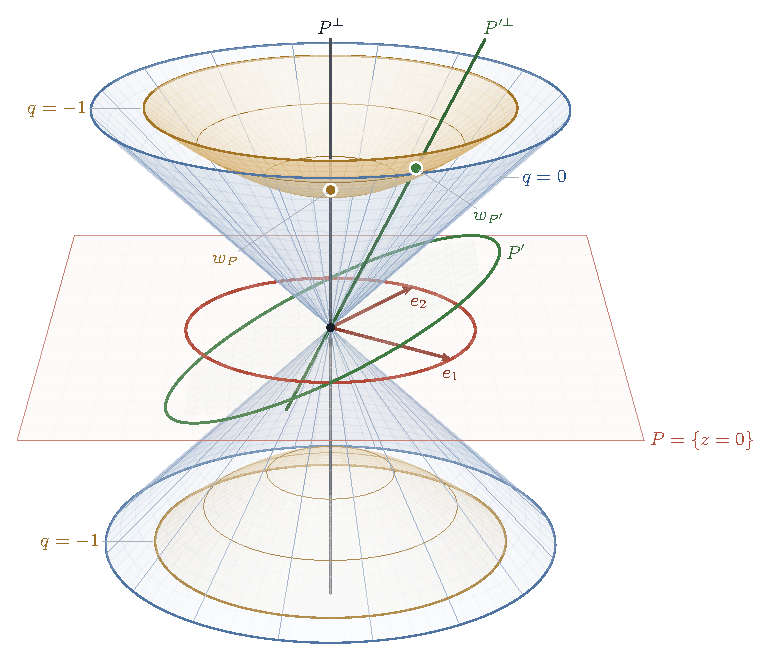
\includegraphics[width=0.88\textwidth]{fig_lightcone}
\caption{The geometry from which the Kuga--Satake construction starts, in the
smallest case $b=3$. The quadratic form is $q=x^{2}+y^{2}-z^{2}$, of
signature $(2,1)$, with its null cone $q=0$; the horizontal plane
$P=\{z=0\}$ is positive definite and meets the cone only at the origin. The
construction needs such a plane, and \Cref{setup:k3type} supplies one:
$P=\langle\Re\sigma,\Im\sigma\rangle$ for the period $\sigma$ spanning
$T^{2,0}$. An orthonormal basis $e_{1},e_{2}$ of $P$ gives $J=e_{1}e_{2}$ with
$J^{2}=-1$ by \Cref{lem:cliffJ}, and $J$ is the complex structure of
$\mathrm{KS}(T)$. A positive definite plane $P$ is determined by the negative
line $P^{\perp}$, which meets the upper sheet of the hyperboloid $q=-1$ in one
point $w_{P}$; that sheet is the period domain, and a second plane $P'$ with
its point $w_{P'}$ is drawn for comparison. The hypothesis behind all of this
is $\dim T^{2,0}=1$, and by \Cref{prop:normpart} an abelian variety of Weil
type with Hodge group $\SU(V,H)$ supplies it in $H^{2}$ only when $n=1$, or
$n=2$ at trivial discriminant.}
\label{fig:ks}
\end{figure}

\section{Reduction to the middle degree}\label{sec:reduction}

The two preceding sections dealt with restriction to hypersurfaces and with
the one classical correspondence that avoids it. Here we combine the first of
them with the Lefschetz decomposition to locate the difficulty of the Hodge
conjecture in general. The result, \Cref{thm:equivalence}, is an equivalence
in which neither side is easier than the other. Its use is to isolate the
primitive classes of middle degree as the one place where a new method is
needed, and by \Cref{thm:hyperplane} restriction to hyperplane sections sees
nothing there.

\subsection{Reduction to primitive classes}

\begin{proposition}[Lefschetz decomposition of Hodge classes]%
\label{prop:lefschetzdecomp}
Let $X$ be smooth projective of dimension $d$ with ample class $L$. Every
$\alpha\in\Hdg^{p}(X)$ can be written
\[
  \alpha=\sum_{r\ge\max(0,\,2p-d)}L^{r}\beta_{r},
  \qquad
  \beta_{r}\in\Hdg^{p-r}(X)\cap H^{2p-2r}_{\mathrm{prim}}(X,\QQ),
\]
and the $\beta_{r}$ are uniquely determined. Consequently the Hodge conjecture
holds for $X$ if and only if every primitive rational Hodge class on $X$ is
algebraic.
\end{proposition}

\begin{proof}
The Lefschetz decomposition
$H^{k}(X,\QQ)=\bigoplus_{r}L^{r}H^{k-2r}_{\mathrm{prim}}(X,\QQ)$ is a
decomposition of rational Hodge structures, because $L$ is a rational class
of type $(1,1)$ and the primitive parts are kernels of morphisms of Hodge
structures. The rationality of $L$ is essential here: for a K\"ahler class
that is not a real multiple of a rational one the primitive subspaces are in
general not rational, and a rational Hodge class need not decompose into
rational primitive pieces. A Hodge class $\alpha$ therefore has Hodge classes
$L^{r}\beta_{r}$ as its components. By hard Lefschetz, $L^{r}$ is injective
on $H^{2p-2r}_{\mathrm{prim}}(X,\QQ)$ for $r\ge\max(0,2p-d)$, and it is a
morphism of Hodge structures of bidegree $(r,r)$, so each $\beta_{r}$ is
uniquely determined and is itself a Hodge class. For the last statement, if
each primitive $\beta_{r}$ is algebraic then so is $L^{r}\beta_{r}$, since $L$
is algebraic and algebraic classes form a subring, and hence so is $\alpha$;
the converse holds because primitive Hodge classes are Hodge classes.
\end{proof}

\subsection{The equivalence}

\begin{theorem}\label{thm:equivalence}
The following are equivalent.
\begin{enumerate}[label=\textup{(\roman*)}]
\item The Hodge conjecture holds for every smooth complex projective variety.
\item The Lefschetz standard conjecture $B(X)$ holds for every smooth complex
  projective variety $X$, and every primitive rational Hodge class of middle
  degree on every smooth complex projective variety of even dimension is
  algebraic.
\end{enumerate}
\end{theorem}

\begin{proof}
(i) implies (ii). The second half of (ii) is a special case of (i). For
$B(X)$, note that $\Lambda$ is a morphism of Hodge structures of bidegree
$(-1,-1)$, hence is given by a Hodge class on $X\times X$ through the
standard correspondence between morphisms of Hodge structures and Hodge
classes on the product, and (i) applied to $X\times X$ makes that class
algebraic. This is Kleiman's argument \cite[\S2]{Kle68}.

(ii) implies (i). We argue by induction on $d=\dim X$. For $d\le1$ the Hodge
conjecture is classical. Let $d\ge2$ and assume the conjecture for all smooth
projective varieties of dimension less than $d$. By Bertini there is a smooth
hypersurface $j\colon Y\hookrightarrow X$ in $|mH|$ for an ample $H$ and
$m\gg0$; put $L=c_{1}(\cO_{X}(Y))$, and take primitivity and the operator
$\Lambda$ with respect to this $L$, which is harmless because $B(X)$ does not
depend on the choice of ample class \cite{Kle68,Kle94}. By
\Cref{prop:lefschetzdecomp} it suffices to prove that a primitive Hodge class
$\alpha\in H^{2p}(X,\QQ)$ is algebraic and, by hard Lefschetz, primitive
classes occur only in degrees at most $d$, so $2p\le d$.

If $2p=d$, then $\alpha$ is a primitive Hodge class of middle degree on a
variety of even dimension, so it is algebraic by the second half of (ii).

If $2p<d$, the class $j^{*}\alpha$ is a rational Hodge class on $Y$ because
$j^{*}$ is a morphism of Hodge structures. As $\dim Y=d-1<d$, the inductive
hypothesis makes $j^{*}\alpha$ algebraic, say $j^{*}\alpha=\cl(W)$ with
$W\in\CH^{p}(Y)_{\QQ}$. Then
$\cl(j_{*}W)=j_{*}j^{*}\alpha=L\alpha$ by \Cref{lem:gysinrestrict}, so
$L\alpha$ is algebraic. By $B(X)$ the operator $\Lambda$ carries algebraic
classes to algebraic classes, and by \Cref{lem:LambdaL},
$\alpha=(d-2p)^{-1}\Lambda(L\alpha)$, which is therefore algebraic; the scalar
is defined because $d-2p\ge1$.
\end{proof}

\begin{remark}[The content of the equivalence]\label{rem:notsimpler}
$B(X)$ is itself a consequence of (i), so
\Cref{thm:equivalence} does not reduce the problem to a smaller one; it
locates the difficulty. The induction in the proof that (ii) implies (i) runs
through every degree except the middle one, where it rests entirely on the
hypothesis. By \Cref{thm:hyperplane}, the step it uses below the middle
degree, restriction to a hypersurface, returns zero on primitive classes of
middle degree, so no refinement of that step extends the induction to that
degree.
\end{remark}

\begin{corollary}[Primitive classes of middle degree]\label{cor:whereidea}
Any proof of the Hodge conjecture must, at some point, produce an algebraic
cycle representing a primitive Hodge class of middle degree on a variety of
even dimension, by a method that does not factor through restriction to
hyperplane sections of that variety.
\end{corollary}

\begin{proof}
By \Cref{thm:equivalence}, the Hodge conjecture includes the algebraicity of
the primitive Hodge classes of middle degree on varieties of even dimension,
and by \Cref{cor:blind} every such class restricts to zero on every smooth
ample hypersurface.
\end{proof}

\begin{remark}[Methods that do not factor through hyperplane sections]%
\label{rem:othermethods}
\Cref{cor:whereidea} does not say that the conjecture is out of reach, and
the settled cases come from known methods outside its scope. The
Kuga--Satake construction (\Cref{sec:ks}) replaces a weight-two Hodge
structure of K3 type by the $H^{1}$ of an abelian variety; the class it
produces is of type $(1,1)$ on a product, hence algebraic by Lefschetz, and it
is not a restriction to a subvariety. Degenerations and limits of Hodge
structures move the variety instead of cutting it. Correspondences from other
varieties, of which the Kuga--Satake construction is one instance and
Markman's construction \cite{Mar25a,Mar25b} another, are also outside the
scope. Arguments through the coniveau filtration, which show that a class
supported on a proper closed subvariety is controlled by that subvariety, are
compatible with everything here: they lower the dimension legitimately,
because the class is supported on the smaller variety, whereas a primitive
class of coniveau zero is supported on no proper closed subvariety.
\end{remark}


\section{Equivariance and Markman's construction}
\label{sec:escape}

We return to abelian varieties of Weil type. By \Cref{thm:character}, a
$\Kx$-eigenclass for the norm character has no component along the Weil line,
and we ask what the contrapositive demands of a construction that does reach
the Weil line. The demand does not concern the size of the object, the ambient
geometry or any dimension count; it concerns the way the object transforms
under $\Kx$. We state it in a concrete form and then show how Markman's
construction meets it.

\subsection{The orbit criterion}

\begin{proposition}[Weil classes generate a plane]\label{prop:orbitplane}
Let $(A,\iota,\eta)$ be of $(K,-1,n)$-Weil type and let $\alpha\in\HW(A)$ be
nonzero. Then
\[
  \mathrm{span}_{\QQ}\bigl\{\iota(\tau)^{*}\alpha\;:\;\tau\in\Kx\bigr\}
  \;=\;\HW(A),
\]
a two-dimensional $\QQ$-vector space, and as a representation of $\Kx$ it is
irreducible over $\QQ$.
\end{proposition}

\begin{proof}
By \Cref{prop:weilline}(i) the space $\HW(A)$ is free of rank one over $K$, and
$\iota(\tau)^{*}$ acts on it as multiplication by the scalar $\tau^{2n}\in K$.
Hence the span in question is $S\cdot\alpha$, where
$S=\mathrm{span}_{\QQ}\{\tau^{2n}:\tau\in\Kx\}\subseteq K$. Taking $\tau=1$
shows $1\in S$. By the argument in the proof of \Cref{lem:charsdiffer} the map
$c(\tau)=\tau/\bbar{\tau}$ has infinite image while $\mu(K)$ is finite, so there
is $\tau_{0}$ with $(\tau_{0}/\bbar{\tau_{0}})^{2n}\ne1$, that is with
$\tau_{0}^{2n}\ne\bbar{\tau_{0}}^{\,2n}$, that is with $\tau_{0}^{2n}\notin\QQ$.
Then $S\supseteq\QQ+\QQ\tau_{0}^{2n}=K$, so $S=K$ and the span is
$K\alpha=\HW(A)$.

For irreducibility, a proper nonzero $\Kx$-stable $\QQ$-subspace would be a
line $\QQ\alpha'$, on which $\Kx$ would act by a $\QQ$-valued character. Since
$\iota(\tau)^{*}\alpha'=\tau^{2n}\alpha'$ and $\HW(A)$ is free over $K$, this forces
$\tau^{2n}\in\QQ$ for all $\tau$, which we have just excluded.
\end{proof}

\begin{corollary}[The orbit criterion]\label{cor:orbitcriterion}
Let $\cE$ be an object of $D^{b}(A)$, or $Z$ a cycle in $\CH^{n}(A)_{\QQ}$,
whose class $\ch_{n}(\cE)$, respectively $\cl(Z)$, is a nonzero Weil class.
Then there is no function $\chi\colon\Kx\to\QQ$ with
\[
  \iota(\tau)^{*}\ch_{n}(\cE)=\chi(\tau)\,\ch_{n}(\cE)
  \qquad\text{for all }\tau\in\Kx .
\]
Equivalently, the $\Kx$-orbit of the class spans a plane and not a line.
\end{corollary}

\begin{proof}
Such a $\chi$ would make $\QQ\cdot\ch_{n}(\cE)$ a $\Kx$-stable line inside
$\HW(A)$, contradicting \Cref{prop:orbitplane}.
\end{proof}

\Cref{cor:orbitcriterion} says in what sense a construction that reaches the
Weil line must break equivariance. Suppose that a construction assigns to the data
$(A,\iota,\eta)$ an object $\cE(A,\iota,\eta)$ naturally, in the sense that
an isomorphism of the data induces an isomorphism of the objects. For
$\tau\ne0$ in the order of $K$ the endomorphism $\iota(\tau)$ is an isogeny of
$A$ commuting with $\iota$ and multiplying $\eta$ by $\Nm(\tau)$, and one
expects naturality to give $\iota(\tau)^{*}\cE\cong\cE$ up to a
normalisation imposed by the change of polarisation, whose effect on
$\ch_{n}$ is multiplication by a rational number $\chi(\tau)$, a power of the
norm. Whenever that is the case, \Cref{cor:orbitcriterion} shows that
$\ch_{n}(\cE)$ is not a nonzero Weil class. A construction that reaches the
Weil line must therefore depend on a choice that $\Gal(K/\QQ)$ moves. The rest
of this section describes such a choice.

\subsection{The two conjugate isotropic subspaces}

The choice that $\Gal(K/\QQ)$ moves is already visible in
\Cref{sec:characters}. The splitting
$V_{\CC}=V_{+}\oplus V_{-}$ of \eqref{eq:Vsplit} is defined over $K$ and not
over $\QQ$, since conjugation interchanges the two summands. Hence
$\bigwedge^{2n}V_{+}$ and $\bigwedge^{2n}V_{-}$ are each defined over $K$,
and only their sum is rational. A class in $\HW(A)$ is of the form
$w+\bbar{w}$ with $w\in\bigwedge^{2n}V_{+}$, and we call $\bigwedge^{2n}V_{+}$
and $\bigwedge^{2n}V_{-}$ the two conjugate halves.

\begin{definition}[Conjugate pair data]\label{def:conjpair}
By \emph{conjugate pair data} for $(A,\iota,\eta)$ we mean a choice of one of
the two summands $V_{\pm}$, equivalently of one of the two embeddings
$K\hookrightarrow\CC$, equivalently of one of the two points of a
$\Gal(K/\QQ)$-orbit of size two attached to the $K$-structure.
\end{definition}

\begin{proposition}[Corestriction produces the plane]\label{prop:corestriction}
Let $w\in\bigwedge^{2n}V_{+}$ be nonzero. Then $w+\bbar{w}$ and
$\sqrt{-d}\,(w-\bbar{w})$ lie in $\HW(A)$ and span it over $\QQ$. In
particular, the rational classes in the Weil line are the
$\Gal(K/\QQ)$-corestrictions of the classes in one conjugate half, and any
construction producing such a class must produce, in effect, a pair of
conjugate inputs and combine them.
\end{proposition}

\begin{proof}
Conjugation interchanges $w$ and $\bbar{w}$ and sends $\sqrt{-d}$ to
$-\sqrt{-d}$, so both elements are fixed by it and are therefore rational.
Both lie in $\bigwedge^{2n}V_{+}\oplus\bigwedge^{2n}V_{-}$ by construction,
hence in $\HW(A)$ by \Cref{def:weilline}. They are linearly independent over
$\QQ$ because $w$ and $\bbar{w}$ are linearly independent over $\CC$: a
relation $q_{1}(w+\bbar{w})+q_{2}\sqrt{-d}\,(w-\bbar{w})=0$ with
$q_{1},q_{2}\in\QQ$ forces $q_{1}+q_{2}\sqrt{-d}=0$, that is $q_{1}=q_{2}=0$.
Since $\HW(A)$ has dimension two by \Cref{prop:weilline}(i), they span it.
\end{proof}

A construction reaching the Weil line therefore has to be, in a suitable
sense, bilinear in the two conjugate halves: it takes one input attached to
$V_{+}$ and one attached to $V_{-}$ and pairs them. A construction fed a
single $K$-invariant input cannot do this, by \Cref{cor:orbitcriterion}.

\subsection{Markman's construction}

Markman's construction \cite{Mar25a,Mar25b} produces Weil classes, and it
meets the criterion in the manner just described. We set out only the
structure relevant here; the details are in \cite{Mar25b}.

The construction does not begin on $A$ or on $\Av$. It begins on an abelian
$n$-fold $X$, that is, on a variety of half the dimension of $A$. Inside
$H^{\mathrm{ev}}(X,\QQ)$ one selects a plane $P$ spanned by Hodge classes, and
one requires that $P$ meet the spinor variety of even pure spinors in two
points. Those two points are conjugate over the imaginary quadratic field $K$;
they correspond to two maximal isotropic subspaces $W_{1}$ and $W_{2}$ that are
interchanged by $\Gal(K/\QQ)$. This is the conjugate pair data of
\Cref{def:conjpair}, realised concretely.

To the two points one attaches \emph{secant sheaves} on $X$, coherent
sheaves whose Chern characters are rational points of $P$. In the worked case
in which $X$ is the Jacobian of a curve of genus three, the secant sheaf is
$\mathcal{I}_{\cup C_{i}}(\Theta)$, the twist by the theta bundle of the ideal
sheaf of a union of translates of the Abel--Jacobi image of the curve. Call the
two sheaves used $\cF_{1}$ and $\cF_{2}$.

The abelian variety of Weil type is then $A=X\times\widehat{X}$, of dimension
$2n$, with its $K$-action and polarisation inherited from $P$. The object that
carries the Weil class is
\begin{equation}\label{eq:markmanobject}
  E=\Phi\bigl(\cF_{1}^{\vee}\boxtimes\cF_{2}\bigr),
\end{equation}
where $\Phi\colon D^{b}(X\times X)\to D^{b}(X\times\widehat{X})$ is Orlov's
derived equivalence. One then shows that the characteristic class $\kappa(E)$
remains of Hodge type under every deformation of $X\times\widehat{X}$ as a
polarised abelian $2n$-fold of Weil type, which is what makes the class
algebraic on the whole family. The conclusion in \cite{Mar25b} is the
algebraicity of the Weil classes for abelian sixfolds of Weil type of trivial
discriminant in the normalisation of \Cref{def:disc} (discriminant $-1$ in
Markman's normalisation), and, through Schoen's product argument
\cite[Proposition~10]{Sch98}, for all abelian fourfolds of Weil type, whence
the Hodge conjecture for abelian fourfolds.

\begin{proposition}[Which hypotheses are escaped]\label{prop:whichescaped}
The object \eqref{eq:markmanobject} satisfies none of the hypotheses of
\Cref{thm:divisor} and does not satisfy the hypothesis of
\Cref{thm:equivsuffices}. Specifically:
\begin{enumerate}[label=\textup{(\roman*)}]
\item \emph{The source is not a projective space.} The input
  $\cF_{1}^{\vee}\boxtimes\cF_{2}$ lives on $X\times X$, an abelian variety.
  The proof of \Cref{thm:divisor} used that $H^{*}(\PP^{N-1},\QQ)$ is generated
  in degree two, so that $\ch$ of any object is a polynomial in the hyperplane
  class. The cohomology of $X\times X$ is not generated in degree two: it
  contains K\"unneth classes of every degree, and $\ch(\cF_{1}^{\vee}\boxtimes\cF_{2})$
  is not confined to any divisor subring.
\item \emph{The transform is not $\Phi_{\cP}$ on $A\times\Av$.} The relevant
  equivalence is between $D^{b}(X\times X)$ and $D^{b}(X\times\widehat{X})$,
  and \Cref{thm:fmtheta}, which computes the transform with Poincar\'e kernel
  on powers of the polarisation of $A$, says nothing about it.
\item \emph{The construction is not $K$-equivariant.} The two tensor factors
  of \eqref{eq:markmanobject} carry the two conjugate points of
  $P\cap(\text{spinor variety})$, one each. Interchanging them is the action of
  the nontrivial element of $\Gal(K/\QQ)$, and it exchanges $E$ with a
  different object. Hence $\ch_{n}(E)$ is not a $\Kx$-eigenclass for the norm,
  and \Cref{cor:orbitcriterion} is satisfied rather than violated.
\end{enumerate}
\end{proposition}

\begin{proof}
Items (i) and (ii) are a comparison of hypotheses and need no argument beyond
reading \eqref{eq:markmanobject}. For (iii), if $\ch_{n}(E)$ were an
eigenclass for the norm, then by \Cref{cor:equivariant} it would have zero
component along the Weil line, whereas Markman shows that this component is
nonzero \cite{Mar25b}.
\end{proof}

The three hypotheses of \Cref{prop:whichescaped} are related. A construction
that takes its input from projective space is normally equivariant for
whatever acts on the input, and an equivariant construction normally returns
a single eigenclass, so the three tend to hold or fail together.

\begin{remark}[Where secant geometry must be placed]\label{rem:secantlesson}
Secant geometry can produce Weil classes: Markman's construction is a secant
construction. The obstructions bear on its placement. Secant geometry placed
on the dual $\Av$ of the $2n$-fold inside an ambient projective space, and
transported by the Poincar\'e kernel, has three defects at once, by
\Cref{prop:whichescaped}: its input lies where the cohomology is generated by
a divisor, it uses the transform to which \Cref{thm:fmtheta} applies, and it
feeds the construction $K$-invariant data, since a secant variety of a
$K$-invariant subvariety is $K$-invariant. Placing the secant geometry on an
abelian $n$-fold removes all three, and it does so because halving the
dimension makes room for the two conjugate inputs.
\end{remark}

\subsection{Beyond the known range}

The algebraicity of the Weil classes is known for $n=2$, for every
discriminant, and for $n=3$ with trivial discriminant; see \cite{Mar25b} and,
for a different route at $n=2$ and trivial discriminant, \cite{FF26}. We state
what a construction of the same shape would have to supply for $n\ge4$.

\begin{question}\label{q:higher}
Fix $n\ge4$ and an imaginary quadratic field $K$. Does there exist an abelian
$n$-fold $X$, a plane $P\subset H^{\mathrm{ev}}(X,\QQ)$ spanned by Hodge
classes meeting the spinor variety in two points conjugate over $K$, secant
sheaves $\cF_{1},\cF_{2}$ on $X$ realising those two points, and a deformation
argument showing that $\kappa\bigl(\Phi(\cF_{1}^{\vee}\boxtimes\cF_{2})\bigr)$
remains of Hodge type across the moduli of polarised abelian $2n$-folds of
Weil type with multiplication by $K$?
\end{question}

Each of the four ingredients is a concrete demand. By
\Cref{cor:orbitcriterion}, any answer must be bilinear in a pair of conjugate
inputs, since that is the only way a rational class can acquire a
$\Kx$-orbit spanning a plane. \Cref{sec:construction} supplies the first three
ingredients explicitly, for every $n\ge2$ and every imaginary quadratic field,
with $X$ an arbitrary polarised abelian $n$-fold. The fourth, the deformation
argument, is isolated in \Cref{rem:deformation}, which says exactly what it
requires.

\begin{figure}[htbp]
\centering
  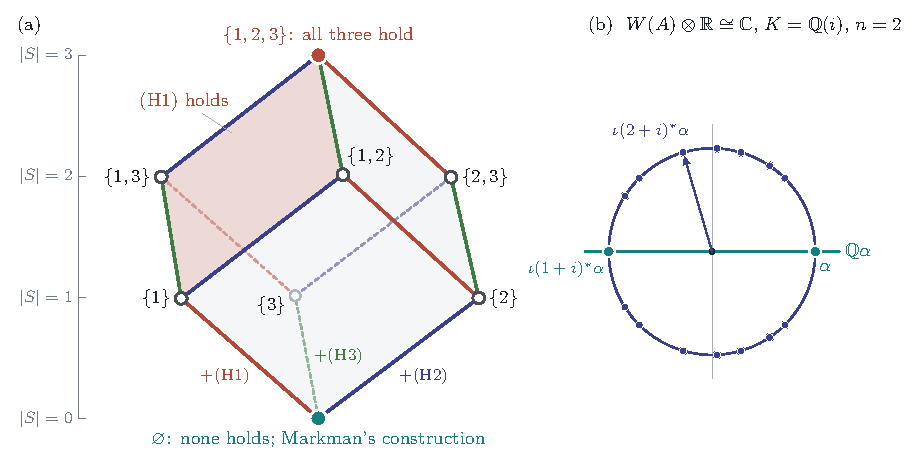
\includegraphics[width=0.97\textwidth]{fig_escape}
\caption{(a) The eight positions a construction can occupy, drawn as the
Boolean lattice of the subsets $S$ of three hypotheses: (H1) the Chern
character of the input lies in the subring generated by divisor classes;
(H2) the output is a $\Kx$-eigenclass; (H3) the output spans a single line
rather than a plane. (H1) and (H2) are the hypotheses negated in (i) and
(iii) of \Cref{prop:whichescaped}, and (H3) is what \Cref{cor:orbitcriterion}
excludes for a nonzero Weil class. At the top vertex all three hold, and both
\Cref{thm:divisor} and \Cref{thm:character} apply; on the shaded face (H1)
holds, and \Cref{thm:divisor} alone already applies. Markman's construction
sits at the bottom vertex, where none of the three holds. (b) The orbit of a
Weil class $\alpha$ under $\Kx$ for $K=\QQ(i)$ and $n=2$, in
$\HW(A)\otimes\RR\cong\CC$ and normalised to the unit circle. Since
$\iota(\tau)^{*}$ acts through $\tau^{4}$, the class $\iota(1+i)^{*}\alpha=-4\alpha$
stays on the line $\QQ\alpha$, while $\iota(2+i)^{*}\alpha$, with
$(2+i)^{4}=-7+24i$, does not; the orbit spans the plane, as
\Cref{prop:orbitplane} asserts.}
\label{fig:escape}
\end{figure}

\section{An explicit secant plane in every dimension}\label{sec:construction}

\Cref{q:higher} asks for four things: an abelian $n$-fold $X$, a plane
$P\subset H^{\mathrm{ev}}(X,\QQ)$ of Hodge classes meeting the spinor variety
in two points conjugate over $K$, a pair of secant sheaves realising the
plane, and a deformation argument. This section supplies the first three, for
every $n\ge2$ and every imaginary quadratic field $K$. The first two are
written in closed form (\Cref{thm:explicitweil,thm:plane}). The third is first
reduced to an explicit equation on a Chern character
(\Cref{thm:secantinvariants}) and then solved, in every dimension, by sheaves
of positive rank whose classes are combinations of the powers of a single line
bundle (\Cref{thm:secantexists}). The fourth ingredient is the deformation
argument, and \Cref{rem:deformation} says exactly what it requires.

The framework is Markman's \cite{Mar25a,Mar25b}: the Weil structure on
$X\times\widehat{X}$ obtained by embedding $K$ into
$\End^{0}(X\times\widehat{X})$, the notion of a $K$-secant sheaf, whose Chern
character lies in a plane meeting the spinor variety at two conjugate points,
and the deformation step that completes the argument at $n=3$ are all his.
What we add is the explicit form of the first three ingredients, uniformly in
$n$ and $K$. The closed form rests on two facts: the two conjugate isotropic
subspaces demanded by \Cref{cor:orbitcriterion} are the graphs of multiples of
a single element of the N\'eron--Severi group, and the pure spinor of the graph
of a two-form is the exponential of that form.

\subsection{The Weil structure}

\begin{setupenv}\label{setup:construction}
Let $X$ be a complex abelian variety of dimension $n$ with
$H_{1}(X,\QQ)=U$ of dimension $2n$ and complex structure $J$ on
$U\otimes\RR$. Let $d$ be a squarefree positive integer, $s=\sqrt{-d}$ and
$K=\QQ(s)$. Let $\beta\in\NS(X)\otimes\QQ$ be nondegenerate, regarded as an
alternating form on $U$, so that the Riemann relation $J^{\top}\beta J=\beta$
holds, and write $\phi_{\beta}\colon X\to\widehat{X}$ for the associated
isogeny. Put
\[
  A=X\times\widehat{X},\qquad \dim A=2n,\qquad
  H_{1}(A,\QQ)=U\oplus U^{\vee},
\]
and let
\begin{equation}\label{eq:Mdef}
  M=\begin{pmatrix}0 & -\beta^{-1}\\[2pt] d\,\beta & 0\end{pmatrix}
  \in\End^{0}(A),
\end{equation}
acting on $H_{1}(A,\QQ)=U\oplus U^{\vee}$ by
$(u,\phi)\mapsto(-\beta^{-1}\phi,\;d\,\beta u)$.
\end{setupenv}

\begin{theorem}[An explicit Weil structure]\label{thm:explicitweil}
In \Cref{setup:construction}:
\begin{enumerate}[label=\textup{(\roman*)}]
\item $M^{2}=-d$, so $\iota(s)=M$ defines an embedding
  $\iota\colon K\hookrightarrow\End^{0}(A)$;
\item $M$ commutes with the complex structure of $A$, and for an
  alternating form $\beta$ on $U$ this is equivalent to the Riemann relation,
  that is to $\beta\in\NS(X)\otimes\QQ$;
\item $M$ acts on $H^{1,0}(A)$ with eigenvalues $s$ and $-s$, each of
  multiplicity $n$, so $(A,\iota,\eta)$ is of $(K,-1,n)$-Weil type for a
  suitable polarisation $\eta$;
\item the eigenspaces $W_{\pm}\subset H_{1}(A,\CC)$ of $M$ for $\pm s$ are
  maximal isotropic for the canonical pairing on $U\oplus U^{\vee}$, are
  interchanged by complex conjugation, and are the graphs of the two-forms
  $\mp s\beta$.
\end{enumerate}
\end{theorem}

\begin{proof}
(i) Block multiplication gives
$M^{2}=\mathrm{diag}(-\beta^{-1}\,d\beta,\;-d\beta\,\beta^{-1})=-d\cdot\mathrm{id}$.

(ii) The complex structure of $A=X\times\widehat{X}$ is
$J_{A}=\mathrm{diag}(J,-J^{\top})$. The relation $MJ_{A}=J_{A}M$ amounts to
the two identities $d\beta J=-dJ^{\top}\beta$ and
$-\beta^{-1}(-J^{\top})=J(-\beta^{-1})$, and each is equivalent to
$\beta J=-J^{\top}\beta$. This is the Riemann relation: from
$J^{\top}\beta J=\beta$ and $J^{2}=-1$ one gets
$J^{\top}\beta=\beta J^{-1}=-\beta J$, as required. Conversely
$\beta J=-J^{\top}\beta$ gives $J^{\top}\beta J=-\beta J J=\beta$.

(iii) $M$ is block anti-diagonal and $H^{1,0}(A)=H^{1,0}(X)\oplus
H^{1,0}(\widehat{X})$ with both summands of dimension $n$, and $M$ exchanges
them. If $M(x,y)=\lambda(x,y)$ then $-\beta^{-1}y=\lambda x$ and
$d\beta x=\lambda y$, so $y=d\beta x/\lambda$ and, substituting,
$-dx/\lambda=\lambda x$, that is $\lambda^{2}=-d$. For each of
the two values of $\lambda$ the assignment $x\mapsto(x,d\beta x/\lambda)$ is an
isomorphism from $H^{1,0}(X)$ onto the $\lambda$-eigenspace, which is
therefore of dimension $n$. That is the balanced signature of
\Cref{def:weiltype}(ii). For (iii) of that definition, let $\eta_{0}$ be any
polarisation of $A$ and put
$\eta(x,y)=\eta_{0}(x,y)+d^{-1}\eta_{0}(Mx,My)$. A positive integer multiple
$mM$ of $M$ is an isogeny, so the second term is the positive multiple
$(dm^{2})^{-1}(mM)^{*}\eta_{0}$ of a polarisation, and $\eta$ is a
polarisation. Since $M^{2}=-d$,
$\eta(Mx,My)=\eta_{0}(Mx,My)+d\,\eta_{0}(x,y)=d\,\eta(x,y)$, and as
$M^{-1}=-M/d$ this gives $\eta(Mx,y)=-\eta(x,My)$: the Rosati involution of
$\eta$ sends $M$ to $-M$, that is $\iota(\tau)^{\dagger}=\iota(\bbar{\tau})$.
When $\beta$ is a polarisation an explicit choice of $\eta$ is recorded in
\Cref{prop:splitgeom}(i).

(iv) The same computation identifies $W_{\lambda}=\{(x,d\beta x/\lambda)\}$,
the graph of the form $d\beta/\lambda$, and
$d\beta/\lambda=d\beta/(\pm s)=\mp s\beta$ since $d/s=-s$. The canonical
pairing on $U\oplus U^{\vee}$ is
$\langle(x,\xi),(x',\xi')\rangle=\xi'(x)+\xi(x')$, and on the graph it gives
$d\beta(x',x)/\lambda+d\beta(x,x')/\lambda=0$ because $\beta$ is alternating; so
$W_{\lambda}$ is isotropic, and it has dimension $2n$, half of
$\dim(U\oplus U^{\vee})=4n$, hence is maximal. Conjugation sends $s$ to $-s$
and so interchanges the two.
\end{proof}

The placement of the factor $d$ in \eqref{eq:Mdef} is a convention, fixed once
and for all. The endomorphism $\begin{psmallmatrix}0&-d\beta^{-1}\\
\beta&0\end{psmallmatrix}$ also squares to $-d$, commutes with the complex
structure and defines a Weil structure on the same $A$, but it is a different
embedding of $K$: its eigenspaces are the graphs of $\mp s\beta/d$ rather
than of $\mp s\beta$, its polarisation is $\beta+d\widehat\beta$ rather than
$d\beta+\widehat\beta$, and the class in
$\bigwedge^{2}V_{+}\oplus\bigwedge^{2}V_{-}$ it produces is
$\beta-d\widehat\beta$ rather than $\gamma=d\beta-\widehat\beta$. The
convention of \eqref{eq:Mdef} is the one whose action on cohomology is
$x\mapsto-Bx$, $\xi\mapsto dB^{-1}\xi$ in the proof of
\Cref{thm:splitclosed}, and every formula below refers to it. For $d=1$ the
two conventions coincide.

\begin{remark}\label{rem:abundant}
\Cref{thm:explicitweil} says that abelian $2n$-folds of Weil type of the split
form $X\times\widehat{X}$ exist for every $n$, every imaginary quadratic $K$
and every polarised abelian $n$-fold $X$, and that the Weil structure is
written down by one element of $\NS(X)$. These are not general members of the
moduli of Weil type. The Weil classes on them are of interest because
Markman's deformation argument, where it can be carried out, propagates
algebraicity from them to the general member; see \Cref{rem:deformation}.
\end{remark}

\subsection{The secant plane}

Write $t=\beta\in\NS(X)\otimes\QQ$, so that by
\Cref{thm:explicitweil}(iv) the two conjugate maximal isotropic subspaces are
the graphs of $\mp s\,t$; we use a separate letter because everything below
holds for any nondegenerate $t\in\NS(X)\otimes\QQ$. The pure spinor
attached to the graph of a two-form $\omega$ is $e^{\omega}$, so the two
conjugate points of the even spinor variety determined by the Weil structure
are $[e^{-st}]$ and $[e^{st}]$.

\begin{definition}[The secant plane]\label{def:secantplane}
With $t$ and $d$ as above, put
\begin{equation}\label{eq:uv}
  u_{t}=\sum_{j\ge0}\frac{(-d)^{j}}{(2j)!}\,t^{2j},
  \qquad
  v_{t}=\sum_{j\ge0}\frac{(-d)^{j}}{(2j+1)!}\,t^{2j+1},
\end{equation}
both sums being finite because $t^{k}=0$ for $k>n$, and let
$P_{t}=\QQ u_{t}\oplus\QQ v_{t}\subset H^{\mathrm{ev}}(X,\QQ)$.
\end{definition}

\begin{theorem}[The plane is an explicit rational secant]\label{thm:plane}
With notation as above:
\begin{enumerate}[label=\textup{(\roman*)}]
\item $u_{t}$ and $v_{t}$ are rational Hodge classes, and
  $e^{\pm st}=u_{t}\pm s\,v_{t}$;
\item $P_{t}$ is a two-dimensional $\QQ$-subspace of $H^{\mathrm{ev}}(X,\QQ)$
  spanned by Hodge classes, and $\PP(P_{t})$ is a line defined over $\QQ$
  passing through the two conjugate points $[e^{\pm st}]$ of the even spinor
  variety;
\item that line is not contained in the spinor variety, so it meets it in
  exactly those two points.
\end{enumerate}
\end{theorem}

\begin{proof}
(i) Each $t^{k}$ is a rational Hodge class because $t\in\NS(X)\otimes\QQ$ is
of type $(1,1)$ and the algebraic classes form a subring. Separating
$e^{st}=\sum_{k}s^{k}t^{k}/k!$ into even and odd powers of $s$ and using
$s^{2j}=(-d)^{j}$, $s^{2j+1}=(-d)^{j}s$ gives $e^{st}=u_{t}+sv_{t}$, and
conjugating gives $e^{-st}=u_{t}-sv_{t}$.

(ii) The two elements are linearly independent over $\QQ$ because $u_{t}$ has
nonzero component in $H^{0}$ and $v_{t}$ does not, while $v_{t}\ne0$ since
$t\ne0$. From (i), both $e^{st}$ and $e^{-st}$ lie in $P_{t}\otimes K$, so
$\PP(P_{t})$ passes through the two points.

(iii) The even spinor variety is cut out by quadrics, by Cartan's description
of pure spinors, so a line either lies inside it or meets it in a subscheme of
length at most two. The point $[u_{t}]$ of $\PP(P_{t})$ is not a pure spinor:
a pure spinor with nonzero component in $H^{0}$ is a scalar multiple of
$e^{\omega}$ for a two-form $\omega$, and $u_{t}$ has zero component in
$H^{2}$ while its component in $H^{4}$ is $-\tfrac{d}{2}t^{2}\ne0$, whereas
$e^{\omega}$ with vanishing $H^{2}$ part is $1$. So the line is not contained
in the spinor variety. The two points of (ii) are distinct, since
$u_{t}+sv_{t}$ and $u_{t}-sv_{t}$ have the same component $1$ in $H^{0}$ and
$v_{t}\ne0$; hence they exhaust the intersection.
\end{proof}

\Cref{fig:spinor} draws the case $n=2$, in which the line $\PP(P_{t})$
meets the spinor quadric in the two conjugate points $[e^{\pm st}]$.

\begin{example}\label{ex:planes}
For $n=4$ and $d=1$,
$u_{t}=1-\tfrac{1}{2}t^{2}+\tfrac{1}{24}t^{4}$ and
$v_{t}=t-\tfrac{1}{6}t^{3}$. For $n=4$ and $d=3$,
$u_{t}=1-\tfrac{3}{2}t^{2}+\tfrac{3}{8}t^{4}$ and
$v_{t}=t-\tfrac{1}{2}t^{3}$. All four classes are rational and lie in the
subring $\QQ[t]$.
\end{example}

\subsection{The Chern character equation}

The next theorem computes the invariants that a sheaf with Chern character in
the secant plane must have. On the side of sheaves, the demands of
\Cref{q:higher} reduce to this one equation.

\begin{theorem}[The invariants of a secant sheaf]\label{thm:secantinvariants}
Let $X$, $t$, $d$ be as above and let $\cF$ be a coherent sheaf on $X$ with
$\ch(\cF)\in P_{t}$, say $\ch(\cF)=a\,u_{t}+b\,v_{t}$ with $a,b\in\QQ$. Then
\[
  \rk\cF=a,\qquad
  c_{1}(\cF)=b\,t,\qquad
  \ch_{2}(\cF)=-\tfrac{ad}{2}\,t^{2},\qquad
  c_{2}(\cF)=\tfrac{ad+b^{2}}{2}\,t^{2},
\]
and more generally $\ch_{k}(\cF)$ is the degree $k$ term of \eqref{eq:uv}
scaled by $a$ or $b$ according to the parity of $k$. The Bogomolov
discriminant is
\begin{equation}\label{eq:discnorm}
  \Delta(\cF)=2a\,c_{2}(\cF)-(a-1)c_{1}(\cF)^{2}
  =\Nm_{K/\QQ}\bigl(b+a s\bigr)\cdot t^{2}.
\end{equation}
In particular, if $t$ is ample and $\cF\ne0$, then
$\Delta(\cF)\cdot H^{n-2}>0$ for every ample $H$, so the Bogomolov inequality
places no obstruction on the existence of $\cF$.
\end{theorem}

\begin{proof}
The first four identities are read off from \eqref{eq:uv} degree by degree,
using $\ch_{2}=\tfrac12(c_{1}^{2}-2c_{2})$ to convert $\ch_{2}$ into $c_{2}$.
For \eqref{eq:discnorm},
\[
  2a\cdot\tfrac{ad+b^{2}}{2}t^{2}-(a-1)b^{2}t^{2}
  =\bigl(a^{2}d+ab^{2}-ab^{2}+b^{2}\bigr)t^{2}
  =\bigl(a^{2}d+b^{2}\bigr)t^{2},
\]
and $\Nm_{K/\QQ}(b+as)=(b+as)(b-as)=b^{2}+a^{2}d$. If $\cF\ne0$ then
$\ch(\cF)\ne0$, so $(a,b)\ne(0,0)$ and the norm is positive; and
$t^{2}H^{n-2}>0$ for $t$ and $H$ ample. This gives the last assertion.
\end{proof}

\begin{remark}[The norm form as the discriminant]\label{rem:normdisc}
Identity \eqref{eq:discnorm} says that the discriminant of the sheaf is the
norm form of $K$ evaluated at the coordinates $(a,b)$ of its Chern character
in the plane. The two conjugate points of the spinor variety are the two
isotropic directions of this norm form after extension of scalars to $K$, and
no nonzero rational point of the plane is isotropic. The Chern character of a
secant sheaf is a rational point of the line $\PP(P_{t})$, and so never an
isotropic one, while the Weil structure is carried by the two isotropic points
of that line, which are defined over $K$. In this sense the conjugate pair of
\Cref{cor:orbitcriterion} is built into the invariants of the sheaf.
\end{remark}

\begin{corollary}[The case of an abelian surface]\label{cor:surfacecase}
Let $n=2$, so $X$ is an abelian surface and $A=X\times\widehat{X}$ an abelian
fourfold of Weil type, and let $t$ be ample. A nonzero sheaf with
$\ch(\cF)\in P_{t}$ has Mukai vector
$v(\cF)=(a,\,bt,\,-\tfrac{ad}{2}t^{2})$ and Mukai self-pairing
\[
  \langle v(\cF),v(\cF)\rangle=\Nm_{K/\QQ}(b+as)\cdot t^{2}>0 .
\]
\end{corollary}

\begin{proof}
On an abelian surface the Mukai pairing of $v=(r,c,e)$ with itself is
$c^{2}-2re$, which here is $b^{2}t^{2}-2a(-\tfrac{ad}{2}t^{2})=(b^{2}+a^{2}d)t^{2}$.
It is positive because $(a,b)\ne(0,0)$ and $t^{2}>0$.
\end{proof}

\Cref{cor:surfacecase} is consistent with the case $n=2$ being settled: on an
abelian surface, positivity of the self-pairing of a primitive Mukai vector of
positive rank is sufficient for the moduli spaces of stable sheaves with that
vector to be non-empty.

\subsection{The genus three Jacobian}

At $n=3$ the equation of \Cref{thm:secantinvariants} determines a secant sheaf
of rank one almost completely, and it reproduces the shape of the object
Markman uses. The computation serves as a check on the framework of this
section.

\begin{proposition}[Rank one at $n=3$]\label{prop:genus3}
Let $X$ be the Jacobian of a smooth curve of genus three, let $\Theta$ be the
theta divisor and $C\subset X$ the Abel--Jacobi curve, so that
$\Theta^{2}/2=[C]$. Take $t=\Theta$ and $a=1$ in
\Cref{thm:secantinvariants}. Then a rank one torsion-free sheaf $\cF$ with
$\ch(\cF)\in P_{\Theta}$ and $c_{1}(\cF)=b\Theta$ is of the form
$\cF=\mathcal{I}_{Z}(b\Theta)$ with
\[
  [Z]=\frac{b^{2}+d}{2}\,\Theta^{2}=(b^{2}+d)\,[C].
\]
If $Z$ is a disjoint union of $m$ translates of $C$, then $b=1$ and
\[
  m=d+1 .
\]
\end{proposition}

\begin{proof}
A rank one torsion-free sheaf on a smooth projective variety is the tensor
product of its double dual, which is a line bundle, with the ideal sheaf of a
subscheme of codimension at least two. With $c_{1}=b\Theta$ this gives
$\cF=\mathcal{I}_{Z}(b\Theta)$ for such a subscheme $Z\subset X$, and
$\ch(\mathcal{I}_{Z}(b\Theta))=e^{b\Theta}\bigl(1-\ch(\cO_{Z})\bigr)$.
Comparing the components in $H^{4}$ with \Cref{thm:secantinvariants} at $a=1$,
which gives $\ch_{2}=-\tfrac{d}{2}\Theta^{2}$, yields
$\tfrac{b^{2}}{2}\Theta^{2}-[Z]=-\tfrac{d}{2}\Theta^{2}$, that is
$[Z]=\tfrac{b^{2}+d}{2}\Theta^{2}$. The Poincar\'e formula
$\Theta^{g-1}/(g-1)!=[C]$ at $g=3$ reads $\Theta^{2}/2=[C]$, whence
$[Z]=(b^{2}+d)[C]$.

Suppose now that $Z$ is a disjoint union of $m$ translates of $C$. Translates
of $C$ are homologous to $C$, so $m=b^{2}+d$. Each translate is a smooth curve
of genus three and $X$ has trivial tangent bundle, so Grothendieck--Riemann--Roch
gives $\ch(\cO_{Z})=m[C]-2m[\mathrm{pt}]$. Using $\Theta^{3}=6[\mathrm{pt}]$
and $\Theta\cdot[C]=3[\mathrm{pt}]$, the component of
$\ch(\mathcal{I}_{Z}(b\Theta))$ in $H^{6}$ is
$(b^{3}-3bm+2m)[\mathrm{pt}]$, and \Cref{thm:secantinvariants} requires it to
equal the degree three term $-bd\,\Theta^{3}/3!=-bd\,[\mathrm{pt}]$.
Substituting $m=b^{2}+d$ gives $-2(b-1)(b^{2}+d)=0$, so $b=1$ and $m=d+1$.
\end{proof}

\begin{table}[htbp]
\centering
\renewcommand{\arraystretch}{1.15}
\begin{tabular}{@{}rrrrrrr@{}}
\toprule
$d$ & $1$ & $2$ & $3$ & $5$ & $7$ & $11$ \\
\midrule
$m=d+1$ & $2$ & $3$ & $4$ & $6$ & $8$ & $12$ \\
\bottomrule
\end{tabular}
\caption{The number $m=d+1$ of translates of the Abel--Jacobi curve in
\Cref{prop:genus3}, as a function of the field $K=\QQ(\sqrt{-d})$.}
\label{tab:translates}
\end{table}

\begin{remark}\label{rem:markmancheck}
The sheaf used in \cite{Mar25b} on a genus three Jacobian is
$\mathcal{I}_{\cup C_{i}}(\Theta)$, the twist by the theta bundle of the ideal
sheaf of a union of translates of the Abel--Jacobi curve. This is the shape
that \Cref{prop:genus3} forces, including the twist by $\Theta$ itself, with
the number of translates determined by the field.
\end{remark}

\subsection{Existence of secant sheaves}\label{ssec:thirdexists}

\Cref{thm:secantinvariants} describes a secant sheaf but does not produce one.
We show that such sheaves exist on every polarised abelian variety, in
every dimension and for every imaginary quadratic field, and that their
classes can be assembled from the powers of a single line bundle.

Two observations do the work. The first is that the Chern character wanted is
a rational point of a plane, and a plane has no preferred scale: a positive
integer multiple $Mp$ of a rational point $p$ of $P_{t}$ is again a rational
point of $P_{t}$, and since the Hodge conjecture concerns classes with
rational coefficients, replacing $p$ by $Mp$ costs nothing. The second is
that, once denominators may be cleared, the Chern characters of the powers of
one line bundle span the subring $\QQ[t]$ in which the secant plane lies,
because the matrix expressing them in the basis $t^{k}/k!$ is a Vandermonde
matrix on distinct nodes. What remains is the passage from a class in $K_{0}$
to a sheaf, and for that the only hypothesis needed is that the rank be
positive.

\begin{lemma}[Positive rank is enough]\label{lem:posrank}
Let $Y$ be a smooth projective variety over a field and let $\alpha\in
K_{0}(Y)$ satisfy $\rk\alpha>0$. Then $\alpha=[\cF]$ for some coherent sheaf
$\cF$ on $Y$.
\end{lemma}

\begin{proof}
Write $m=\dim Y$ and $a=\rk\alpha\ge1$, and let $F^{c}K_{0}(Y)$ be the
topological filtration, the subgroup generated by the classes $[\cO_{Z}]$ of
closed integral subschemes $Z\subseteq Y$ of codimension at least $c$. Since
$Y$ is smooth, every coherent sheaf has a finite locally free resolution, so
$K_{0}(Y)=K_{0}'(Y)$ and the filtration is exhaustive with $F^{m+1}=0$.
The class of a coherent sheaf supported in codimension at least $c$
lies in $F^{c}$ and is congruent modulo $F^{c+1}$ to
$\sum_{i}\ell_{i}[\cO_{Z_{i}}]$, where $\sum_{i}\ell_{i}Z_{i}$ is its cycle in
codimension $c$; and $F^{1}$ is the kernel of the rank, while $F^{1}/F^{2}$ is
$\Pic(Y)$ through the first Chern class \cite[\S 15.1 and
Ex.~15.1.5]{Ful98}. We construct coherent
sheaves $\cF_{c}$ of rank $a$ with $\alpha-[\cF_{c}]\in F^{c}$, by induction on
$c$.

Start at $c=2$. Let $L$ be a line bundle with $c_{1}(L)=c_{1}(\alpha)$ and set
$\cF_{2}=L\oplus\cO_{Y}^{\oplus(a-1)}$. Then $\alpha-[\cF_{2}]$ has rank zero
and first Chern class zero, hence lies in $F^{2}$.

For the inductive step let $\delta=\alpha-[\cF_{c}]\in F^{c}$ with $c\ge2$.
Modulo $F^{c+1}$ the class $\delta$ is a finite sum $\sum_{j}m_{j}
[\cO_{Z_{j}}]$ with $m_{j}\in\ZZ$ and $\codim Z_{j}=c$. The terms with
$m_{j}>0$ are removed by replacing $\cF_{c}$ with $\cF_{c}\oplus\bigoplus_{
m_{j}>0}\cO_{Z_{j}}^{\oplus m_{j}}$, which changes neither the rank nor the
codimension of the remaining difference. For a term with $m_{j}<0$ we must
subtract, and here the rank is used. The restriction $\cF_{c}\otimes
\cO_{Z_{j}}$ is a quotient of $\cF_{c}$ and has rank at least $a\ge1$ at the
generic point of the integral scheme $Z_{j}$, by semicontinuity of the fibre
dimension. Dividing $\cF_{c}\otimes\cO_{Z_{j}}$ by a subsheaf of generic
corank one gives a surjection $\cF_{c}\twoheadrightarrow\cQ$ with $\cQ$ a
coherent $\cO_{Z_{j}}$-module of rank one. Then $[\cQ]\in F^{c}$ with
associated cycle $[Z_{j}]$, so $[\cQ]-[\cO_{Z_{j}}]\in F^{c+1}$. The kernel of
that surjection is a coherent sheaf, still of rank $a$ because $\cQ$ is
supported in positive codimension, and its class is $[\cF_{c}]-[\cQ]$.
Performing this $|m_{j}|$ times for each $j$ with $m_{j}<0$ produces
$\cF_{c+1}$ with $\alpha-[\cF_{c+1}]\in F^{c+1}$ and $\rk\cF_{c+1}=a$. At
$c=m+1$ the difference lies in $F^{m+1}=0$, so $\alpha=[\cF_{m+1}]$.
\end{proof}

\begin{theorem}[Secant sheaves exist in every dimension]\label{thm:secantexists}
Let $X$ be an abelian variety of dimension $n$, let $t\in\NS(X)\otimes\QQ$ be a
polarisation and let $d>0$. Let $p$ be a rational point of the secant plane
$P_{t}$ whose $u_{t}$ coordinate is positive. Then there are a positive
integer $M$, an integer $D>0$ with $Dt\in\NS(X)$, integers $n_{0},\dots,n_{n}$
and a coherent sheaf $\cF$ on $X$ such that, setting
\begin{equation}\label{eq:lbwitness}
  \alpha=\sum_{j=0}^{n}n_{j}\bigl[\cO_{X}(jDt)\bigr]\in K_{0}(X),
\end{equation}
one has $\alpha=[\cF]$ in $K_{0}(X)$, $\ch(\cF)=M\,p$ and
$\rk\cF=M\,a>0$, where $a$ is the $u_{t}$ coordinate of $p$. The integers $M$
and $n_{j}$ depend only on $n$, $d$, $D$ and the coordinates of $p$, and are
obtained by inverting one Vandermonde matrix. Moreover $Mp$ is again a
rational point of $P_{t}$; applying the statement to two linearly independent
rational points of $P_{t}$ produces a pair of coherent sheaves whose Chern
characters span $P_{t}$.
\end{theorem}

\begin{proof}
If the conclusion holds for $Np$, where $N$ is a positive integer, with
multiple $M'$, then it holds for $p$ with $M=NM'$, and the hypothesis on $p$
is unchanged by the scaling. Clearing the denominators of the coordinates of
$p$, we may therefore assume $p=au_{t}+bv_{t}$ with $a,b\in\ZZ$ and $a>0$.
Choose $D>0$ with $Dt\in\NS(X)$, so that $\cO_{X}(jDt)$ is a line bundle for
every $j\in\ZZ$.

Since $t$ is a polarisation, $t^{n}\ne0$ and $t^{n+1}=0$ in
$H^{\mathrm{ev}}(X,\QQ)$, so the $n+1$ classes $t^{k}/k!$ with $0\le k\le n$
are a basis of the subring $\QQ[t]$. In that basis
\[
  p=\sum_{k=0}^{n}c_{k}\,\frac{t^{k}}{k!},\qquad
  c_{k}=\begin{cases}a(-d)^{k/2}, & k\ \text{even},\\[2pt]
                     b(-d)^{(k-1)/2}, & k\ \text{odd},\end{cases}
\]
by \eqref{eq:uv}, and all the $c_{k}$ are integers. On the other
side,
\[
  \ch\bigl(\cO_{X}(jDt)\bigr)=e^{jDt}=\sum_{k=0}^{n}(jD)^{k}\,\frac{t^{k}}{k!},
\]
so in the same basis the $n+1$ vectors $\ch(\cO_{X}(jDt))$ for $j=0,\dots,n$
are the columns of the Vandermonde matrix $\bigl((jD)^{k}\bigr)_{0\le j,k\le n}$
on the $n+1$ distinct nodes $0,D,2D,\dots,nD$. Its determinant is
$\prod_{0\le i<j\le n}(jD-iD)=D^{n(n+1)/2}\prod_{0\le i<j\le n}(j-i)\ne0$, so
the system
\[
  \sum_{j=0}^{n}x_{j}\,(jD)^{k}=c_{k}\qquad(0\le k\le n)
\]
has a unique solution $x\in\QQ^{n+1}$. Let $M$ be the least common multiple of
the denominators of the $x_{j}$ and put $n_{j}=Mx_{j}\in\ZZ$. With $\alpha$ as
in \eqref{eq:lbwitness},
\[
  \ch(\alpha)=\sum_{j}n_{j}e^{jDt}
  =\sum_{k=0}^{n}\Bigl(\sum_{j}Mx_{j}(jD)^{k}\Bigr)\frac{t^{k}}{k!}
  =M\sum_{k=0}^{n}c_{k}\frac{t^{k}}{k!}=Mp .
\]
In particular $\rk\alpha=\ch_{0}(\alpha)=Mc_{0}=Ma>0$, so \Cref{lem:posrank}
gives a coherent sheaf $\cF$ with $[\cF]=\alpha$. The Chern character is a
function of the class in $K_{0}(X)$, whence $\ch(\cF)=Mp$ and $\rk\cF=Ma$.
Finally $Mp=(Ma)u_{t}+(Mb)v_{t}$ is a rational point of $P_{t}$, and two
linearly independent rational points stay linearly independent after scaling,
which gives the last assertion.
\end{proof}

\Cref{fig:moment} draws the theorem at $n=2$ and $d=2$, with the points of
the secant plane that integer combinations of line bundles reach.

\begin{remark}[The factorials and the multiple $M$]%
\label{rem:themultiple}
The integer $M$ is not an artefact of the proof. The lattice spanned by the
Chern characters of the powers of a single line bundle is spanned equally well
by the classes $(e^{t}-1)^{k}$ for $0\le k\le n$, because the $(n+1)$st finite
difference of a polynomial of degree $n$ vanishes; and $(e^{t}-1)^{k}=t^{k}+
\cdots$ has leading term $t^{k}$, not $t^{k}/k!$. The secant plane, by
contrast, is spanned by classes whose coordinates in the basis $t^{k}/k!$ are
integers. The index between the two lattices can be computed exactly. Write
$j^{k}=\sum_{i\le k}S(k,i)\,i!\binom{j}{i}$ with the Stirling numbers $S(k,i)$
of the second kind. As $j$ runs over $0,\dots,n$, the vectors
$\bigl(\binom{j}{i}\bigr)_{0\le i\le n}$ form a unitriangular basis of
$\ZZ^{n+1}$, so the vectors $(j^{k})_{0\le k\le n}$, which are the coordinates
of $\ch\cO_{X}(jt)$ in the basis $t^{k}/k!$, span the image of $\ZZ^{n+1}$
under the lower triangular matrix $T=\bigl(S(k,i)\,i!\bigr)_{k,i}$, whose
diagonal is $0!,1!,\dots,n!$. The index is therefore $\prod_{k\le n}k!$. The
inverse of $T$ is $\bigl(s(k,i)/k!\bigr)_{k,i}$, with the Stirling numbers
$s(k,i)$ of the first kind, because $\binom{j}{k}=\sum_{i}s(k,i)j^{i}/k!$;
so $n!\,T^{-1}$ is integral, and for every integral point $p$ of the secant
plane the least admissible $M$ divides $n!$. It is often larger than $1$. At $n=4$, $d=3$, $a=b=1$ the least multiple is $M=6$,
a divisor of $4!$, and the witness is
\[
  \alpha=-23\,[\cO_{X}]+66\,[\cO_{X}(t)]-54\,[\cO_{X}(2t)]
         +20\,[\cO_{X}(3t)]-3\,[\cO_{X}(4t)],
\]
of rank $-23+66-54+20-3=6=Ma$; in degree one its coefficient is
$66-108+60-12=6=Mb$, and in degrees two to four the sums
$\sum_{j}n_{j}j^{k}$ are $-18$, $-18$ and $54$, which are $6c_{2}$, $6c_{3}$ and
$6c_{4}$. The solution of the Vandermonde system is unique and the $n_{j}$
have no common factor, $23$ being prime to $6$, so $M=6$ is the least
multiple, and the freedom to rescale is needed. \Cref{fig:multiple} shows
the least multiple in further cases.

For a principal polarisation $\theta$ the classes $\theta^{k}/k!$ are
integral: in a symplectic basis $x_{1},\dots,x_{g},y_{1},\dots,y_{g}$ of
$H^{1}(X,\ZZ)$, $\theta=\sum_{i}x_{i}y_{i}$, the products $x_{i}y_{i}$
commute and square to zero, and so
$\theta^{k}/k!=\sum_{|I|=k}\prod_{i\in I}x_{i}y_{i}$. This is Poincar\'e's
formula in a form that does not need a curve, and it is why $t^{k}/k!$ is the
natural integral basis in which to take the coordinates $c_{k}$.
\end{remark}

\begin{figure}[htbp]
\centering
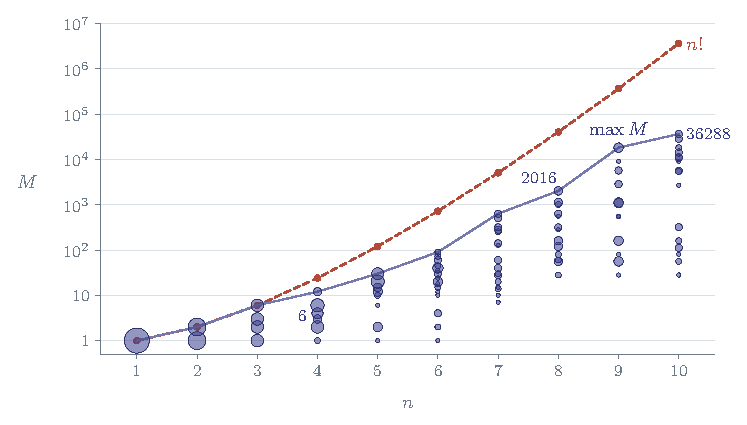
\includegraphics[width=0.85\textwidth]{fig_multiple}
\caption{\Cref{rem:themultiple}. The least multiple $M$ of
\Cref{thm:secantexists} for $1\le n\le10$, over the seventy-two cases
$d\in\{1,2,3,5,7,11\}$, $a\in\{1,2,3\}$, $b\in\{\pm1,\pm2\}$ for each
$n$, read off from the solution of the Vandermonde system, on a logarithmic
scale; the area of a disc counts the cases with that value. The solid line
joins the largest values and the dashed one is $n!$, which every $M$ divides
by the remark: the quotient of $\ZZ^{n+1}$ by the lattice of the
characters $(1,j,\dots,j^{n})$ of the powers of a line bundle is dual to the
integer-valued polynomials of degree at most $n$, spanned by the
$\binom{x}{k}$, whose coefficients have denominators dividing $n!$.}
\label{fig:multiple}
\end{figure}

\begin{figure}[htbp]
\centering
  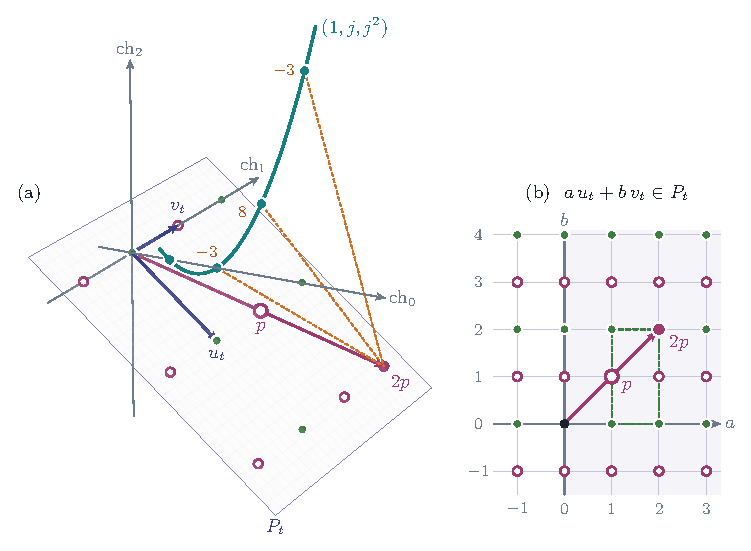
\includegraphics[width=0.86\textwidth]{fig_moment}
\caption{\Cref{thm:secantexists} at $n=2$ and $d=2$. (a) The coordinates
$(\ch_{0},\ch_{1},\ch_{2})$ in the basis $1$, $t$, $t^{2}/2$. The Chern
characters of the powers of one line bundle lie on the moment curve
$j\mapsto(1,j,j^{2})$, and the Vandermonde determinant says that any three of
its points are affinely independent. The integral points of
$P_{t}=\QQ u_{t}\oplus\QQ v_{t}$ split by the criterion
$\ch_{2}\equiv\ch_{1}\bmod2$ into those reached by integer combinations of
line bundles, drawn filled, and those missed, drawn open. The point
$p=u_{t}+v_{t}$ is missed and $2p$ is reached, by the witness
$-3[\cO_{X}]+8[\cO_{X}(t)]-3[\cO_{X}(2t)]$, whose three terms are joined to
$2p$ by dashed segments. (b) The same points in the coordinates $(a,b)$ of
$a\,u_{t}+b\,v_{t}$. Here $\ch_{1}=b$ and $\ch_{2}=-2a$, so the criterion reads
$b\equiv0\bmod2$; the shaded half-plane $a>0$ is the range of
\Cref{thm:secantexists}.}
\label{fig:moment}
\end{figure}

\subsection{The three ingredients}

\begin{theorem}[Three of the four ingredients]\label{thm:twoofthefour}
For every $n\ge2$, every squarefree $d>0$ and every polarised abelian $n$-fold
$X$ carrying a nondegenerate $\beta\in\NS(X)\otimes\QQ$, the first three of the
four ingredients required by \Cref{q:higher} exist and are explicit:
\begin{enumerate}[label=\textup{(\alph*)}]
\item the abelian $2n$-fold of Weil type is $A=X\times\widehat{X}$ with the
  $K$-action \eqref{eq:Mdef}, by \Cref{thm:explicitweil};
\item the plane is $P_{t}$ of \Cref{def:secantplane} with $t=\beta$, it is
  spanned by Hodge classes and it meets the spinor variety in exactly the two
  conjugate points $[e^{\pm st}]$, by \Cref{thm:plane};
\item a pair of coherent sheaves $\cF_{1},\cF_{2}$ on $X$ whose Chern
  characters are linearly independent rational points of $P_{t}$ exists, by
  \Cref{thm:secantexists}, and each may be taken to have the class of an
  explicit integer combination of powers of one line bundle.
\end{enumerate}
The invariants of any such sheaf are forced by the explicit system of
\Cref{thm:secantinvariants}, which imposes $n-1$ linear conditions on a Chern
character already constrained to $\QQ[t]$, and, when $\beta$ is ample, are
unobstructed numerically by \eqref{eq:discnorm}.
\end{theorem}

\begin{proof}
Items (a), (b) and (c) are the cited theorems. For (c), the proof of
\Cref{thm:secantexists} uses of $t$ only that $t^{n}\ne0$ and that a positive
multiple of $t$ is integral; both hold for $t=\beta$, the first because
$\beta$ is nondegenerate. For the count in the last sentence, a Chern
character in the subring $\QQ[t]\subset H^{\mathrm{ev}}(X,\QQ)$ is a
polynomial of degree at most $n$ in $t$, so lies in a space of dimension
$n+1$, while $P_{t}$ has dimension two, and $(n+1)-2=n-1$.
\end{proof}

\begin{remark}[The deformation step]\label{rem:deformation}
The fourth ingredient of \Cref{q:higher} is untouched by this section, and it
is the hardest. Given the pair of secant sheaves $\cF_{1},\cF_{2}$ on $X$
supplied by \Cref{thm:secantexists}, one must still show that the
characteristic class of $\Phi(\cF_{1}^{\vee}\boxtimes\cF_{2})$ remains of
Hodge type under every deformation of $X\times\widehat{X}$ as a polarised
abelian $2n$-fold of Weil type, and that the object deforms with the variety,
as a twisted sheaf to first order. Markman carries out this step at $n=3$
\cite{Mar25b}, through a semiregularity analysis. Our contribution to it is
negative: \cite[Theorem~4.56]{paperII} identifies the Hochschild classes that the
weakened form of that analysis must kill for a secant object, and
\cite[Theorem~4.61]{paperII} shows that the candidate Markman proposes for $n=4$
does not kill them. Without the step one obtains algebraicity only on the
split locus $X\times\widehat{X}$, where the Weil classes are of much less
interest, since the general abelian $2n$-fold of Weil type is simple and is
not of that form.

Accordingly, nothing in this section proves the Hodge conjecture for abelian
$2n$-folds of Weil type at any $n\ge4$. What is established is that three of
the four ingredients are written down for every $n$, the third with an
explicit witness in line bundles, and that the fourth is isolated.
\end{remark}

\begin{figure}[htbp]
\centering
  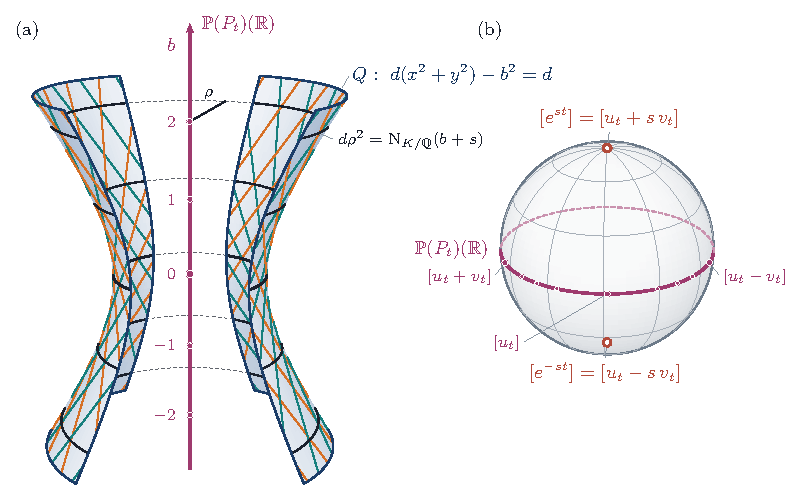
\includegraphics[width=0.88\textwidth]{fig_quadric}
\caption{The geometry of \Cref{thm:plane} in the first case, $n=2$. The even
spinor variety is then the smooth six-dimensional quadric of classes
isotropic for the Mukai pairing in $\PP(H^{\mathrm{ev}}(X,\CC))\cong\PP^{7}$,
and the figure shows a real two-dimensional section of it, a quadric surface
with its two rulings. The line $\PP(P_{t})$ of \Cref{def:secantplane} is
defined over $\QQ$ and meets the quadric only in the two points
$[e^{\pm st}]$, which are conjugate over $K$ and not individually rational;
they are drawn as real points. This is the configuration the Weil line
demands: a class defined over $\QQ$ cannot single out one of the two points,
so the construction must carry the pair, and the pair spans a plane rather
than a line. \Cref{prop:orbitplane} is the same statement on the
cohomological side, and \Cref{fig:escape} places it among the hypotheses a
construction can satisfy.}
\label{fig:spinor}
\end{figure}

\section{Base points in every Weil family}\label{sec:basepoints}

The secant construction of \Cref{sec:construction} lives on the split variety
$X\times\widehat{X}$ and stops short of the deformation step. In this section
we study the split member and the other special members of a Weil family
through the Weil classes themselves. On the split member the Weil classes are
polynomials in three divisor classes (\Cref{thm:splitclosed}); on products of
abelian surfaces of Weil type they are polynomials in divisor classes
(\Cref{thm:everyn}); and on abelian varieties with quaternionic
multiplication extending $K$, and on their products, they are polynomials in
two divisor classes, which yields an algebraic base point in every Weil
family, of every discriminant (\Cref{thm:everyfamily}). What remains is the
propagation of one flat class over one connected period domain, formulated
in \Cref{ssec:residual,ssec:exactform}.

\subsection{The split member in closed form}\label{ssec:split}

We begin with the split member, where a single formula, valid for every $n$
and every $d$, writes the Weil classes as polynomials in three divisor
classes. The split locus is thin. A general abelian $2n$-fold
of Weil type is simple, hence not isogenous to a product, and for $n\ge2$ the
members $X\times\widehat{X}$ form a subvariety of $\cD_{n,n}$ of positive
codimension (\Cref{prop:splitgeom}(iii)). \Cref{cor:splitalgebraic} is
therefore a base case, and \Cref{q:residual} is a question about propagation.

\begin{notation}\label{not:threeclasses}
On $A=X\times\widehat{X}$ write
\[
  \beta\in H^{2}(A,\QQ),
  \qquad
  \widehat{\beta}\in H^{2}(A,\QQ),
  \qquad
  \ell=c_{1}(\cP)\in H^{2}(A,\QQ)
\]
for the pullback of the polarisation of $X$, the pullback of the dual
polarisation of $\widehat{X}$, and the class of the Poincar\'e bundle. All
three are divisor classes, so every polynomial in them is algebraic. Put
\begin{equation}\label{eq:gammadef}
  \gamma=d\,\beta-\widehat{\beta}.
\end{equation}
\end{notation}

\begin{theorem}[The Weil line of the split member]\label{thm:splitclosed}
Let $A=X\times\widehat{X}$ carry the $K$-action \eqref{eq:Mdef} determined by a
principal $\beta$, and let $V_{\pm}\subset H^{1}(A,\CC)$ be the eigenspaces of
$\iota(\sqrt{-d})$. Then
\begin{enumerate}[label=\textup{(\roman*)},nosep]
\item $\gamma\mp\sqrt{-d}\,\ell$ lies in $\bigwedge^{2}V_{\pm}$, so it is an
  eigenclass for the character $\tau\mapsto\tau^{2}$ on $H^{2}(A,\CC)$
  respectively for its conjugate;
\item the generators of $\bigwedge^{2n}V_{\pm}$ are
  \begin{equation}\label{eq:splitclosed}
    \omega_{\pm}
    =\frac{(-1)^{n(n-1)/2}}{n!\,d^{\,n}}
      \bigl(\gamma\mp\sqrt{-d}\,\ell\bigr)^{n};
  \end{equation}
\item consequently the Weil line of $A$ is
  \[
    \HW(A)=\Bigl\langle\;
      \Re\bigl(\gamma-\sqrt{-d}\,\ell\bigr)^{n},\;\;
      \Im\bigl(\gamma-\sqrt{-d}\,\ell\bigr)^{n}
    \;\Bigr\rangle_{\QQ},
  \]
  and every Weil class on $A$ is a polynomial with rational coefficients in
  the three divisor classes $\beta,\widehat{\beta},\ell$, hence is algebraic.
\end{enumerate}
\end{theorem}

\begin{proof}
Write $U=H^{1}(X,\QQ)$ with basis $x_{1},\dots,x_{2n}$ chosen so that
$\beta=\sum_{j\le n}x_{j}\wedge x_{n+j}$, let $\xi_{1},\dots,\xi_{2n}$ be the
dual basis of $H^{1}(\widehat{X},\QQ)=U^{\vee}$, and let $B\colon U\to U^{\vee}$
be the isomorphism induced by $\beta$, so that $Bx_{j}=\xi_{n+j}$ and
$Bx_{n+j}=-\xi_{j}$. The endomorphism \eqref{eq:Mdef} acts on homology, and
its transpose $M^{*}$ acts on $H^{1}(A,\QQ)=U\oplus U^{\vee}$ by
$u\mapsto -Bu$ and $\phi\mapsto d\,B^{-1}\phi$. Indeed, in the basis
$u_{1},\dots,u_{2n}$ of $H_{1}(X,\QQ)$ dual to the $x_{i}$, the map
$\beta\colon H_{1}(X)\to H^{1}(X)$ sends $u_{j}\mapsto x_{n+j}$ and
$u_{n+j}\mapsto-x_{j}$, so \eqref{eq:Mdef} sends $u_{j}\mapsto dx_{n+j}$,
$u_{n+j}\mapsto-dx_{j}$, $x_{n+j}\mapsto-u_{j}$ and $x_{j}\mapsto u_{n+j}$,
where $x_{i}$ is regarded as an element of
$H_{1}(\widehat X,\QQ)=H^{1}(X,\QQ)$ and $\xi_{i}$ is its dual class; pairing
with the dual basis gives the stated action. The square of $M^{*}$ is $-d$;
so, writing $\delta=\sqrt{-d}$,
\begin{equation}\label{eq:splitVpm}
  V_{\pm}=\Bigl\{\,u\pm\tfrac{\delta}{d}\,Bu\;:\;u\in U_{\CC}\Bigr\},
\end{equation}
since $M^{*}\bigl(u\pm\tfrac{\delta}{d}Bu\bigr)
=-Bu\pm\delta u=\pm\delta\bigl(u\pm\tfrac{\delta}{d}Bu\bigr)$.

(i) Take the sum over $j\le n$ of the wedges of the two eigenvectors attached
to $x_{j}$ and to $x_{n+j}$:
\[
  \sum_{j=1}^{n}
  \Bigl(x_{j}\pm\tfrac{\delta}{d}Bx_{j}\Bigr)\wedge
  \Bigl(x_{n+j}\pm\tfrac{\delta}{d}Bx_{n+j}\Bigr)
  =\beta\pm\tfrac{\delta}{d}\Sigma-\tfrac{1}{d}\widehat{\beta},
\]
using $\delta^{2}=-d$, where
$\Sigma=\sum_{j}\bigl(x_{j}\wedge Bx_{n+j}+Bx_{j}\wedge x_{n+j}\bigr)$ and
$\sum_{j}Bx_{j}\wedge Bx_{n+j}=\sum_{j}\xi_{n+j}\wedge(-\xi_{j})
=\widehat{\beta}$. Now
\[
  \Sigma=\sum_{j=1}^{n}\bigl(x_{j}\wedge(-\xi_{j})
        +\xi_{n+j}\wedge x_{n+j}\bigr)
   =-\sum_{i=1}^{2n}x_{i}\wedge\xi_{i}=-\ell .
\]
So the displayed sum is $\tfrac1d\bigl(d\beta-\widehat{\beta}\mp\delta\ell\bigr)
=\tfrac1d(\gamma\mp\delta\ell)$. It is a sum of wedges of pairs of vectors of
$V_{\pm}$, hence lies in $\bigwedge^{2}V_{\pm}$, which proves (i); the
statement about characters is \Cref{prop:grading} at $(r,s)=(2,0)$ and
$(0,2)$.

(ii) By (i) the $n$-th power $(\gamma\mp\delta\ell)^{n}$ lies in
$\bigwedge^{2n}V_{\pm}$, which is a line by \Cref{prop:weilline}. It is
nonzero: expanding $\gamma\mp\delta\ell=d\beta-\widehat{\beta}\mp\delta\ell$,
the only term of the $n$-th power lying in $\bigwedge^{2n}U$ is
$d^{\,n}\beta^{n}$, and $\beta^{n}\ne0$ because $\beta$ is nondegenerate;
the remaining terms all involve at least one $\xi$, so no cancellation can
occur. Hence $(\gamma\mp\delta\ell)^{n}$ spans $\bigwedge^{2n}V_{\pm}$ and is a
scalar multiple of $\omega_{\pm}=\bigwedge_{i=1}^{2n}\bigl(x_{i}\pm\tfrac{\delta}{d}Bx_{i}\bigr)$.
To find the scalar, compare the components in $\bigwedge^{2n}U$: that of
$\omega_{\pm}$ is $x_{1}\wedge\cdots\wedge x_{2n}$, while
\[
  d^{\,n}\beta^{n}=d^{\,n}\,n!\bigwedge_{j=1}^{n}(x_{j}\wedge x_{n+j})
  =d^{\,n}\,n!\,(-1)^{n(n-1)/2}\,x_{1}\wedge\cdots\wedge x_{2n},
\]
the sign being that of the permutation carrying
$(1,n+1,2,n+2,\dots,n,2n)$ to $(1,2,\dots,2n)$. Inverting gives
\eqref{eq:splitclosed}.

(iii) The two displayed classes are the real and imaginary parts of
$(\gamma-\delta\ell)^{n}$, which up to the nonzero rational factor in
\eqref{eq:splitclosed} are $\omega_{-}+\omega_{+}$ and
$(\omega_{-}-\omega_{+})/\delta$; by \Cref{prop:weilline}(i) these span
$\HW(A)$ over $\QQ$. Expanding $(\gamma-\delta\ell)^{n}$ by the binomial
theorem and separating even from odd powers of $\delta$ writes each of them as
a rational polynomial in $\beta,\widehat{\beta},\ell$, because
$\delta^{2m}=(-d)^{m}$ and $\delta^{2m+1}=(-d)^{m}\delta$. Products of divisor
classes are algebraic, so both are algebraic.
\end{proof}

\begin{example}\label{ex:splitsmall}
The $2n$ classes $x_{1},\dots,x_{2n}$ form a $K$-basis of $H^{1}(A,\QQ)$, on
which $\sqrt{-d}$ acts by $x\mapsto-Bx$, so \eqref{eq:omegaprod} applies to
them; with \eqref{eq:splitclosed} it gives the integral generators of
\Cref{thm:explicitgens} for this basis in closed form,
\[
  \omega_{1}+\sqrt{-d}\,\omega_{2}
  =\frac{(-1)^{n(n-1)/2}}{n!}\,\bigl(\gamma+\sqrt{-d}\,\ell\bigr)^{n}.
\]
At $n=2$ this reads
\[
  \omega_{1}=\tfrac12\bigl(d\,\ell^{2}-\gamma^{2}\bigr),
  \qquad
  \omega_{2}=-\gamma\,\ell,
\]
and at $n=3$,
\[
  \omega_{1}=\tfrac12\,d\,\gamma\,\ell^{2}-\tfrac16\gamma^{3},
  \qquad
  \omega_{2}=\tfrac16\,d\,\ell^{3}-\tfrac12\gamma^{2}\ell,
\]
with $\gamma=d\beta-\widehat{\beta}$ throughout.
\end{example}

\begin{corollary}[Algebraicity on the split locus]\label{cor:splitalgebraic}
For every $n\ge1$, every squarefree $d>0$ and every principally polarised
abelian $n$-fold $X$, the Weil classes of $A=X\times\widehat{X}$ with the
$K$-action \eqref{eq:Mdef} are algebraic, and an algebraic representative is
given by \eqref{eq:splitclosed} as an explicit rational combination of
intersections of three divisors.
\end{corollary}

\begin{proof}
This is \Cref{thm:splitclosed}(iii), together with the Lefschetz theorem on
$(1,1)$ classes, which makes $\beta,\widehat{\beta},\ell$ algebraic, and the
fact that the algebraic classes form a subring of $H^{*}(A,\QQ)$.
\end{proof}

\begin{remark}[Consistency with the character obstruction]\label{rem:splitconsistent}
\Cref{cor:splitalgebraic} does not contradict \Cref{thm:character}. At the
split point $\NS(A)\otimes\QQ$ contains the three independent classes
$\beta,\widehat{\beta},\ell$, so the hypothesis
$\NS(A)\otimes\QQ=\QQ\eta$ of \Cref{prop:notpoly} fails, and this is the
situation of \cite[Remark~2.5]{paperIII}. What \Cref{thm:character} forbids is a
$\Kx$-eigenclass for the norm character meeting the Weil line, and
$\gamma\mp\sqrt{-d}\,\ell$ is an eigenclass for $\tau^{2}$ and for
$\bbar{\tau}^{2}$, not for the norm. The formula \eqref{eq:splitclosed} is
the first place in the paper where a class in the relevant eigenspace is
exhibited, and such a class exists because the split member has enough
divisors to build one.
\end{remark}

\subsection{Products of abelian surfaces}\label{ssec:products}

A second source of members with enough divisors is the product, an operation
that the Weil line respects. Throughout this subsection $K$ is fixed and all
Weil structures are taken with respect to it.

\begin{lemma}[Products of Weil type]\label{lem:prodweil}
Let $(A_{1},\iota_{1},\eta_{1})$ be of $(K,-1,n_{1})$-Weil type and
$(A_{2},\iota_{2},\eta_{2})$ of $(K,-1,n_{2})$-Weil type. Then
$A=A_{1}\times A_{2}$, with the diagonal action
$\iota=\iota_{1}\times\iota_{2}$ and the product polarisation
$\eta=p_{1}^{*}\eta_{1}+p_{2}^{*}\eta_{2}$, is of
$(K,-1,n_{1}+n_{2})$-Weil type.
\end{lemma}

\begin{proof}
Write $V_{i}=H^{1}(A_{i},\QQ)$, so $V=H^{1}(A,\QQ)=V_{1}\oplus V_{2}$ as
$K$-vector spaces and $\dim_{K}V=2n_{1}+2n_{2}$. The Rosati involution of the
product polarisation is the product of the two Rosati involutions, so it
restricts on $K$ to conjugation, which is the sign $-1$ of
\Cref{def:weiltype}. For the multiplicities, the Hodge decomposition of $V$ is
the direct sum of those of $V_{1}$ and $V_{2}$, and the eigenspace
decomposition is likewise $V_{\pm}=V_{1,\pm}\oplus V_{2,\pm}$. Hence
\[
  \dim_{\CC}V_{+}^{1,0}
  =\dim_{\CC}V_{1,+}^{1,0}+\dim_{\CC}V_{2,+}^{1,0}
  =n_{1}+n_{2},
\]
and the same for the other three, which is \Cref{lem:balanced} for
$n=n_{1}+n_{2}$.
\end{proof}

For an abelian variety $A$ of $(K,-1,n)$-Weil type and a $K$-basis of
$H^{1}(A,\QQ)$, let $\omega_{1}(A),\omega_{2}(A)$ be the generators of the
Weil line given by \eqref{eq:omegagens} in that basis, and write
\[
  \omega(A)=\omega_{1}(A)+\sqrt{-d}\,\omega_{2}(A)\;\in\;
  K\otimes_{\QQ}H^{2n}(A,\QQ)
\]
for the $K$-valued Weil class; by \eqref{eq:omegaprod} its image in
$H^{2n}(A,\CC)$ is $d^{-n}\prod_{j}(d\,x_{j}+\delta\,y_{j})$. On a product we
use the $K$-basis obtained by concatenating bases of the factors.

The Weil line is the top exterior power over $K$, and a top exterior power of
a direct sum is the tensor product of the top exterior powers. This is the
content of the next theorem; what has to be checked is its effect on the
rational generators, which are defined through the real structure rather
than over $K$.

\begin{theorem}[The Weil class is multiplicative]\label{thm:weilmult}
With the notation of \Cref{lem:prodweil}, and cup product on
$H^{*}(A,\QQ)$ taken after pullback along the two projections,
\begin{equation}\label{eq:weilmult}
\begin{aligned}
  \omega_{1}(A)&=\omega_{1}(A_{1})\,\omega_{1}(A_{2})
    -d\,\omega_{2}(A_{1})\,\omega_{2}(A_{2}),\\
  \omega_{2}(A)&=\omega_{1}(A_{1})\,\omega_{2}(A_{2})
    +\omega_{2}(A_{1})\,\omega_{1}(A_{2}),
\end{aligned}
\end{equation}
that is $\omega(A_{1})\,\omega(A_{2})=\omega(A_{1}\times A_{2})$ for the
$K$-valued Weil class. For $k$ factors,
$\prod_{j}\omega(A_{j})=\omega(A_{1}\times\cdots\times A_{k})$.
\end{theorem}

\begin{proof}
Let $u_{1},\dots,u_{2n_{1}}$ and $u_{2n_{1}+1},\dots,u_{2n}$ be the
$K$-bases of $H^{1}(A_{1},\QQ)$ and $H^{1}(A_{2},\QQ)$, so that together they
form the $K$-basis of $H^{1}(A,\QQ)$, and put $x_{j}=u_{j}$ and
$y_{j}=\sqrt{-d}\,u_{j}$ as in \eqref{eq:omegaprod}. By \eqref{eq:omegaprod},
\[
\begin{aligned}
  \omega(A)
  &=d^{-n}\prod_{j=1}^{2n}\bigl(d\,x_{j}+\delta\,y_{j}\bigr)\\
  &=\Bigl(d^{-n_{1}}\prod_{j\le2n_{1}}\bigl(d\,x_{j}+\delta\,y_{j}\bigr)\Bigr)
   \Bigl(d^{-n_{2}}\prod_{j>2n_{1}}\bigl(d\,x_{j}+\delta\,y_{j}\bigr)\Bigr)
  =\omega(A_{1})\,\omega(A_{2})
\end{aligned}
\]
in $H^{2n}(A,\CC)$, the products being taken in the order of the basis, so
that no sign arises. Expanding
$\bigl(\omega_{1}(A_{1})+\delta\omega_{2}(A_{1})\bigr)
\bigl(\omega_{1}(A_{2})+\delta\omega_{2}(A_{2})\bigr)$ with $\delta^{2}=-d$,
and comparing rational parts and $\delta$-parts, which is legitimate because
the classes $\omega_{j}(A_{i})$ are rational and $1,\delta$ are linearly
independent over $\QQ$, gives \eqref{eq:weilmult}. The statement for $k$
factors follows by induction.
\end{proof}

\Cref{fig:product} shows the multiplicativity and the loci it reaches.

\begin{corollary}[Algebraicity propagates along products]\label{cor:prodalg}
If the Weil classes of $A_{1}$ and of $A_{2}$ are algebraic, then so are those
of $A_{1}\times A_{2}$, and an algebraic representative is the rational
combination of external products given by \eqref{eq:weilmult}.
\end{corollary}

\begin{proof}
Algebraic classes are closed under pullback along the projections and under
cup product, and \eqref{eq:weilmult} expresses $\omega_{1}(A)$ and
$\omega_{2}(A)$ in those operations applied to the $\omega_{j}(A_{i})$.
\end{proof}

In dimension two there is nothing to prove.

\begin{lemma}[Dimension two]\label{lem:basecase}
Let $A_{0}$ be of $(K,-1,1)$-Weil type, so $\dim A_{0}=2$. Then
$\HW(A_{0})\subset H^{2}(A_{0},\QQ)$ and both generators are algebraic.
\end{lemma}

\begin{proof}
The Weil classes lie in $H^{2n}=H^{2}$ and are of type $(1,1)$ by
\Cref{prop:weilline}(ii), so they are algebraic by the Lefschetz theorem on
$(1,1)$ classes. No hypothesis on $A_{0}$ beyond the Weil structure is used.
\end{proof}

\begin{theorem}[An algebraic Weil class in every dimension]\label{thm:everyn}
Let $n\ge1$, let $d>0$ be squarefree, and let $A_{1},\dots,A_{n}$ be abelian
surfaces of $(K,-1,1)$-Weil type. Then $A=A_{1}\times\cdots\times A_{n}$ is of
$(K,-1,n)$-Weil type and its Weil classes are algebraic; explicitly, by
\Cref{thm:weilmult} and \Cref{lem:basecase} they are the rational part and
the coefficient of $\sqrt{-d}$ in
$\prod_{j=1}^{n}\bigl(\omega_{1}(A_{j})+\sqrt{-d}\,\omega_{2}(A_{j})\bigr)$,
a polynomial with integer coefficients in $2n$ divisor classes.
\end{theorem}

\begin{proof}
\Cref{lem:prodweil} gives the Weil structure, \Cref{lem:basecase} gives
algebraicity of each factor's classes, and \Cref{cor:prodalg} applied $n-1$
times gives the conclusion; the displayed form is \Cref{thm:weilmult} for $k=n$
factors. Each $\omega_{j}(A_{i})$ is a divisor class by
\Cref{lem:basecase}, so the product is a polynomial in $2n$ of them.
\end{proof}

\begin{remark}[The product locus]\label{rem:prodscope}
\Cref{thm:everyn} is unconditional and holds for every $n$; like
\Cref{cor:splitalgebraic} and \Cref{thm:everyfamily}, it produces an algebraic
Weil class in every dimension using nothing beyond the Lefschetz theorem on
$(1,1)$ classes. The product construction supplies a second family of base
points, defined for every $n$ and every $d$, at which the class is written
down explicitly. It also shows that the algebraicity locus is closed under
products, so that a settled case $n_{0}$ propagates to every multiple of
$n_{0}$, and settled cases propagate to their sums. Combined with Markman's
theorem at $n=2$ \cite{Mar25a,Mar25b}, this gives, for every $n$,
algebraicity on the locus of products of abelian fourfolds and surfaces of
Weil type, which has dimension $2n$ when $n$ is even.

The reach of these results is limited. The family of polarised abelian
$2n$-folds of $(K,-1,n)$-Weil type has dimension $n^{2}$, and the locus of
products of $n$ surfaces has dimension $n$, so for $n\ge2$ it is a proper
closed subvariety, smaller than the quaternionic locus of \Cref{thm:quatweil},
whose dimension is $n(n+1)/2$. A general member of the family is simple,
hence not isogenous to a product, and neither \Cref{thm:everyn} nor
\Cref{cor:splitalgebraic} applies to it. The general member lies outside all
of these loci, and by \Cref{thm:residual} what joins them to it is the
propagation statement.
\end{remark}

\begin{figure}[htbp]
\centering
  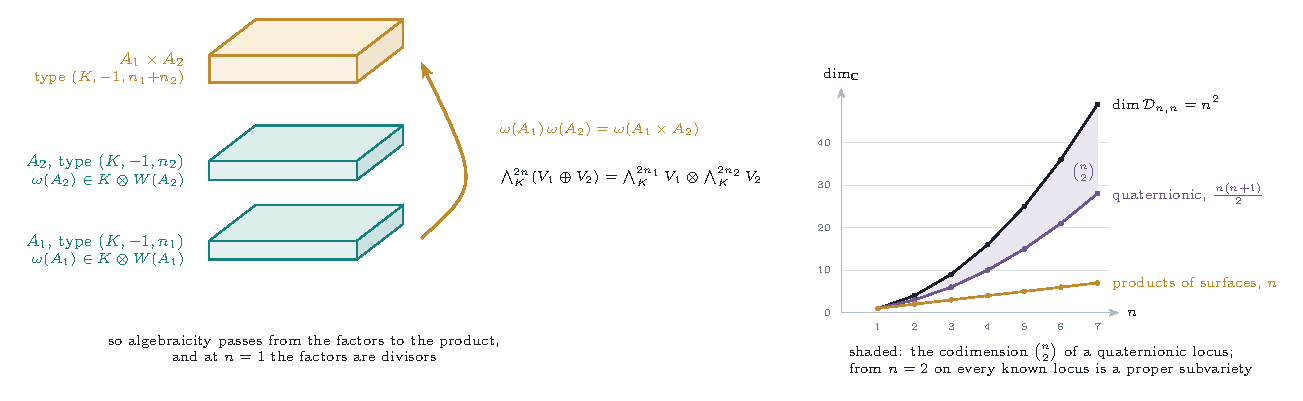
\includegraphics[width=0.96\textwidth]{fig_product}
\caption{\Cref{thm:weilmult} and its reach. Left: the Weil line of each factor
is a $K$-line, the Weil line of the product is the tensor product of the two
over $K$, and the $K$-valued Weil class is multiplicative. Algebraicity therefore passes from the factors to the product, and
at $n=1$ the factors are divisor classes, so a product of $n$ abelian surfaces
of Weil type carries an explicit algebraic Weil class in every dimension.
Right: the dimensions of the loci on which the class is known to be algebraic,
against the dimension $n^{2}$ of the family. Both the quaternionic locus and
the product locus are proper subvarieties once $n\ge2$, and a general member
lies on neither.}
\label{fig:product}
\end{figure}

\subsection{The residual statement}\label{ssec:residual}

The results above allow the remaining question to be stated in one sentence,
without auxiliary hypotheses.

\begin{setupenv}[The family]\label{setup:family}
Fix $n\ge2$ and a squarefree $d>0$. Let $\cD_{n,n}$ be the period domain of
\Cref{prop:weildomain} and let
\[
  \pi\colon\cA\longrightarrow\cD_{n,n}
\]
be the family of polarised abelian $2n$-folds of $(K,-1,n)$-Weil type it
parametrises, with $\omega$ the flat section of $R^{2n}\pi_{*}\QQ$ given
fibrewise by the class $\omega_{1}$ of \eqref{eq:omegagens}. Let
$\cD^{\mathrm{spl}}\subset\cD_{n,n}$ be the locus of split members
$X\times\widehat{X}$ carrying the action \eqref{eq:Mdef}.
\end{setupenv}

\begin{question}[The residual statement]\label{q:residual}
Is $\omega_{s}$ algebraic for every $s\in\cD_{n,n}$?
\end{question}

\begin{theorem}[The reduction]\label{thm:residual}
Fix $n\ge2$ and a squarefree $d>0$, and keep the notation of
\Cref{setup:family}.
\begin{enumerate}[label=\textup{(\alph*)},nosep]
\item If \Cref{q:residual} has a positive answer, then the Hodge conjecture
  holds, in every degree, for every abelian $2n$-fold of $(K,-1,n)$-Weil type
  with $\Hg(A)=\SU(V,H)$.
\item Conversely, if the Hodge conjecture holds for every abelian $2n$-fold of
  $(K,-1,n)$-Weil type, then \Cref{q:residual} has a positive answer.
\item $\cD^{\mathrm{spl}}$ is nonempty, $\omega_{s}$ is algebraic at every
  $s\in\cD^{\mathrm{spl}}$ with the explicit representative
  \eqref{eq:splitclosed}, and $\cD_{n,n}$ is connected.
\end{enumerate}
Thus \Cref{q:residual} is the variational Hodge conjecture for one flat class
on one connected family; it is necessary as well as sufficient, and its base
case is supplied. \Cref{thm:everyfamily} supplies a base case in every family,
for every discriminant, so nonemptiness of the base locus is never the
obstacle.
\end{theorem}

\begin{proof}
(a) Let $A$ be of $(K,-1,n)$-Weil type with $\Hg(A)=\SU(V,H)$. By
\Cref{prop:weildomain} its Hodge structure is a point $s$ of $\cD_{n,n}$, so
$A$ is a fibre of $\pi$, and the Weil line of $A$ is generated over $K$ by
$\omega_{s}$. A positive answer makes $\omega_{s}$ algebraic, hence makes the
whole Weil line algebraic by the argument of \Cref{cor:whatisleft}. By
\Cref{thm:hdgcount} the Weil line together with the powers of $\eta$ exhausts
$\Hdg^{*}(A)$, and the powers of $\eta$ are algebraic, so every Hodge class on
$A$ is algebraic.

(b) For every $s$ the class $\omega_{s}$ is a Hodge class on the fibre $A_{s}$,
by \Cref{prop:weilline}(ii), and $A_{s}$ is of $(K,-1,n)$-Weil type by
construction. So the Hodge conjecture for $A_{s}$ gives its algebraicity.

(c) $\cD^{\mathrm{spl}}$ is nonempty because the construction \eqref{eq:Mdef}
applies to any principally polarised abelian $n$-fold and produces a point of
$\cD_{n,n}$ by \Cref{thm:explicitweil}; algebraicity there is
\Cref{cor:splitalgebraic}; and $\cD_{n,n}$ is connected because it is a
bounded symmetric domain, by \Cref{prop:weildomain}.
\end{proof}

\begin{remark}[The target]\label{rem:target}
The preceding sections remove three parts of the problem.
\Cref{thm:hdgcount} settles how many classes are at issue: one, in one
degree, on each fibre. \Cref{thm:divisor} and \Cref{thm:character} exclude
two families of candidate constructions. \Cref{thm:splitclosed} supplies the
base case: the class is algebraic somewhere in the family, with a
representative that can be written on a single line.

The next step is propagation, which is Grothendieck's variational Hodge
conjecture for the pair $(\pi,\omega)$ of \Cref{setup:family}.
\Cref{thm:residual} shows that for the Hodge conjecture on
abelian varieties of Weil type it is necessary as well as sufficient, so every
route to the conjecture meets an equivalent difficulty.
\Cref{ssec:properness} analyses the propagation; there the passage from a
formal deformation to an algebraic one, usually the harder half, is supplied
by properness of the Hilbert scheme. What survives is either an infinitesimal
statement at a single point or a bound on the complexity of representing
cycles along one orbit, and the second is equivalent to its conclusion
(\Cref{thm:p1equivalent}).
\end{remark}

\subsection{The divisorial criterion}
\label{ssec:divcrit}

\Cref{thm:splitclosed} is a computation on one member of the family, but the
mechanism behind it is not special to that member. Isolating it gives a
criterion that can be tested at any point; we then determine where it holds.

\begin{theorem}[The divisorial criterion]\label{thm:divcriterion}
Let $(A,\iota,\eta)$ be of $(K,-1,n)$-Weil type and suppose there exists
$\Theta\in\bigwedge^{2}V_{-}$ with
\begin{enumerate}[label=\textup{(\roman*)},nosep]
\item $\Theta$ nondegenerate as an alternating form on $V_{-}^{\vee}$,
  equivalently $\Theta^{n}\ne0$;
\item $\Theta$ of Hodge type $(1,1)$;
\item $\Theta+\bbar{\Theta}$ rational, that is in $H^{2}(A,\QQ)$.
\end{enumerate}
Then the Weil classes of $A$ are algebraic. Explicitly, writing
$g=\Theta+\bbar{\Theta}$ and $\lambda=(\Theta-\bbar{\Theta})/\sqrt{-d}$, both
$g$ and $\lambda$ are divisor classes and
\begin{equation}\label{eq:divrep}
  \HW(A)=\Bigl\langle\;
    \Re\bigl(g+\sqrt{-d}\,\lambda\bigr)^{n},\;\;
    \Im\bigl(g+\sqrt{-d}\,\lambda\bigr)^{n}\;\Bigr\rangle_{\QQ},
\end{equation}
so every Weil class is a rational polynomial in two divisor classes.
\end{theorem}

\begin{proof}
Conjugation interchanges $\bigwedge^{2}V_{-}$ and $\bigwedge^{2}V_{+}$, so
$\bbar{\Theta}\in\bigwedge^{2}V_{+}$, and both $g$ and $\lambda$ are fixed by
conjugation, hence real. Rationality of $g$ is (iii); that of $\lambda$
comes from the action of $\Kx$. Fix
$\tau=a+b\sqrt{-d}\in\Kx$ with $ab\ne0$. By \Cref{prop:grading} the operator
$\iota(\tau)^{*}$ acts on $\bigwedge^{2}V_{+}$ by $\tau^{2}=a^{2}-db^{2}+2ab\sqrt{-d}$
and on $\bigwedge^{2}V_{-}$ by $\bbar{\tau}^{\,2}$, so
\[
  J:=\frac{\iota(\tau)^{*}-(a^{2}-db^{2})}{2ab}
\]
is a $\QQ$-rational endomorphism of $H^{2}(A,\QQ)$ preserving the space $R$
of \Cref{prop:normpart} and acting
on $\bigwedge^{2}V_{\pm}$ by $\pm\sqrt{-d}$. Applying it to
$g=\Theta+\bbar{\Theta}$ gives $J(g)=-\sqrt{-d}\,\Theta+\sqrt{-d}\,\bbar{\Theta}
=-\sqrt{-d}\cdot\sqrt{-d}\,\lambda=d\,\lambda$, so $\lambda=J(g)/d$ is
rational. Both $g$ and $\lambda$ are of type $(1,1)$ by (ii) and conjugation
symmetry, so both lie in $\NS(A)\otimes\QQ$ by the Lefschetz theorem on
$(1,1)$ classes, and both are algebraic.

By (i) the form $\Theta$ on the $2n$-dimensional space $V_{-}$ has nonzero
Pfaffian, so $\Theta^{n}$ is a nonzero element of the line
$\bigwedge^{2n}V_{-}$, and it therefore spans it; conjugating,
$\bbar{\Theta}^{\,n}$ spans $\bigwedge^{2n}V_{+}$. Hence
$\Theta^{n}+\bbar{\Theta}^{\,n}$ and
$(\Theta^{n}-\bbar{\Theta}^{\,n})/\sqrt{-d}$ span $\HW(A)$ over $\QQ$, by
\Cref{prop:weilline}(i). Finally
$2^{n}\Theta^{n}=(g+\sqrt{-d}\lambda)^{n}$, and expanding by the binomial
theorem with $(\sqrt{-d})^{2m}=(-d)^{m}$ writes the real and imaginary parts
as rational polynomials in $g$ and $\lambda$. Products of divisor classes are
algebraic.
\end{proof}

\begin{corollary}\label{cor:splitsatisfies}
The split member of \Cref{thm:splitclosed} satisfies the criterion, with
$\Theta=\gamma-\sqrt{-d}\,\ell$ and $\gamma=d\beta-\widehat{\beta}$; the two
divisor classes of \eqref{eq:divrep} are $2\gamma$ and $-2\ell$.
\end{corollary}

\begin{proof}
\Cref{thm:splitclosed}(i) places $\Theta=\gamma-\sqrt{-d}\,\ell$ in
$\bigwedge^{2}V_{+}$ and its conjugate in $\bigwedge^{2}V_{-}$. The hypotheses
and the conclusion of \Cref{thm:divcriterion} are symmetric under replacing
$\Theta$ by $\bbar{\Theta}$, which interchanges $V_{+}$ and $V_{-}$, fixes $g$
and changes the sign of $\lambda$, so the criterion may be applied to
$\Theta$. The classes $\gamma$ and $\ell$ are divisor classes, hence of type
$(1,1)$, so $\Theta$ is of type $(1,1)$ and $\Theta+\bbar{\Theta}=2\gamma$ is
rational. Nondegeneracy is the nonvanishing of $\Theta^{n}$, proved in
\Cref{thm:splitclosed}(ii).
\end{proof}

The base case is therefore one instance of a general criterion. The next two
results determine how far the criterion reaches, and both limit it.

\begin{proposition}[The criterion fails at a general point]\label{prop:divfails}
Let $(A,\iota,\eta)$ be of $(K,-1,n)$-Weil type with $n\ge2$ and
$\Hg(A)=\SU(V,H)$. Put
\[
  R=\Bigl(\textstyle\bigwedge^{2}V_{+}\oplus\bigwedge^{2}V_{-}\Bigr)
      \cap H^{2}(A,\QQ).
\]
Then $R\cap\NS(A)_{\QQ}=0$, and no $\Theta$ as in \Cref{thm:divcriterion}
exists.
\end{proposition}

\begin{proof}
By \Cref{prop:normpart} the space $R$ is a rational sub-Hodge structure of
$H^{2}(A,\QQ)$, and the intersection $R\cap\NS(A)_{\QQ}$ is a rational
sub-Hodge structure of $R$ of pure type $(1,1)$. The complexification of a
nonzero rational sub-Hodge structure of $R$ is a nonzero
$\Hg(A)_{\CC}$-subrepresentation of $\bigwedge^{2}V_{+}\oplus\bigwedge^{2}V_{-}$,
so it contains a constituent isomorphic to $\bigwedge^{2}V_{+}$ or to
$\bigwedge^{2}V_{-}$; by the proof of \Cref{prop:normpart}, Hodge numbers
depend only on the representation, and by \Cref{prop:h2pieces} each of
$\bigwedge^{2}V_{\pm}$ has $h^{2,0}+h^{0,2}=2\binom{n}{2}=n(n-1)$, which is
positive for $n\ge2$. So no nonzero rational sub-Hodge structure of $R$ is of
pure type $(1,1)$, and $R\cap\NS(A)_{\QQ}=0$. The argument covers the case
$n=2$ with trivial discriminant, where $R$ is reducible. A $\Theta$ as in
\Cref{thm:divcriterion} would give the nonzero element $\Theta+\bbar{\Theta}$
of $R\cap\NS(A)_{\QQ}$.
\end{proof}

\begin{proposition}[The split locus]\label{prop:splitgeom}
Fix $n\ge1$ and a squarefree $d>0$, and let $A=X\times\widehat{X}$ carry the
$K$-action \eqref{eq:Mdef} determined by a nondegenerate
$\beta\in\NS(X)\otimes\QQ$ of elementary divisors $(d_{1},\dots,d_{n})$.
\begin{enumerate}[label=\textup{(\roman*)},nosep]
\item Let $B$ be the Gram matrix of $\beta$ in a basis of $U$, and let
  $\widehat\beta$ be the form on $U^{\vee}$ with Gram matrix $-B^{-1}$ in the
  dual basis, which for principal $\beta$ is the class of
  \Cref{not:threeclasses}. The polarisation of $A$ is
  $\eta=\beta+\widehat{\beta}/d$, a positive rational multiple of
  $d\beta+\widehat\beta$; its Gram matrix on $H_{1}(A,\QQ)=U\oplus U^{\vee}$
  is the block form $Q=B\oplus(-B^{-1}/d)$, and $M$ is anti-self-adjoint for
  it.
\item In the $K$-basis $u_{1},\dots,u_{2n}$ of $H_{1}(A,\QQ)$ the hermitian
  form of \Cref{lem:hermform} has Gram matrix $\sqrt{-d}\,B$, so
  \[
    \det H=(-d)^{n}\det B=(-d)^{n}(d_{1}\cdots d_{n})^{2},
  \]
  and $(-1)^{n}\det H=d^{\,n}(d_{1}\cdots d_{n})^{2}$ is a norm from $K$.
  Every split member therefore lies in the Weil family of trivial
  discriminant, whatever $\beta$ is chosen.
\item The split members form a locus of dimension $n(n+1)/2$ inside
  $\cD_{n,n}$, of codimension $n(n-1)/2$, which is zero only for $n=1$ and is
  a divisor for $n=2$.
\item For $X$ with $\Hg(X)=\mathrm{Sp}(H^{1}(X,\QQ))$ one has
  $\NS(A)_{\QQ}=\langle\beta,\widehat{\beta},\ell\rangle$, of rank three, and
  in degree $2n$ the monomials in those three classes span the whole space of
  Hodge classes of $A$.
\end{enumerate}
\end{proposition}

\begin{proof}
(i) In the chosen basis of $U$ and the dual basis of $U^{\vee}$ the map
$\beta\colon U\to U^{\vee}$ has matrix $B^{\top}=-B$ and its inverse has
matrix $-B^{-1}$, so \eqref{eq:Mdef} becomes
$M=\begin{psmallmatrix}0&B^{-1}\\-dB&0\end{psmallmatrix}$, with
$M^{2}=-d$ and
$M^{\top}=\begin{psmallmatrix}0&dB\\-B^{-1}&0\end{psmallmatrix}$, using
$B^{\top}=-B$ and $(B^{-1})^{\top}=-B^{-1}$. For a block form
$Q=\begin{psmallmatrix}P&\Lambda\\-\Lambda^{\top}&S\end{psmallmatrix}$ the
Rosati relation $M^{\top}Q+QM=0$ reads
$B\Lambda^{\top}+\Lambda B=0$, $dBS+PB^{-1}=0$, $B^{-1}P+dSB=0$ and
$B^{-1}\Lambda+\Lambda^{\top}B^{-1}=0$. Taking $\Lambda=0$ and $P=B$ forces
$S=-B^{-1}/d$ from the second relation, and the third then reads $-I+I=0$.
So $Q=B\oplus(-B^{-1}/d)$, which is the Gram matrix of
$\beta+\widehat\beta/d$. For principal $\beta$ one may take
$B=\begin{psmallmatrix}0&I\\-I&0\end{psmallmatrix}$, so that $-B^{-1}=B$
and $\widehat\beta=\sum_{j}\xi_{j}\wedge\xi_{n+j}$ as in
\Cref{not:threeclasses}.

(ii) The set $u_{1},\dots,u_{2n}$ is a $K$-basis because
$MU=d\beta(U)=U^{\vee}$, and $H(u_{i},u_{j})=Q(Mu_{i},u_{j})+\sqrt{-d}\,Q(u_{i},u_{j})$
by \eqref{eq:QfromH}; the first term vanishes since $Mu_{i}\in U^{\vee}$,
$u_{j}\in U$ and $Q$ has no cross block by (i), and the second is
$\sqrt{-d}\,\beta_{ij}$. Hence the Gram matrix is $\sqrt{-d}\,B$ and
$\det H=(\sqrt{-d})^{2n}\det B=(-d)^{n}\det B$. The determinant of an
alternating matrix is the square of its Pfaffian, here $(d_{1}\cdots
d_{n})^{2}$. Now $d=\Nm_{K/\QQ}(\sqrt{-d})$ is a norm and every square is a
norm, and the norms form a subgroup of $\QQ^{\times}$, so
$d^{\,n}(d_{1}\cdots d_{n})^{2}$ is a norm.

(iii) A split member is determined by $X$ together with $\beta$; the moduli
space of polarised abelian $n$-folds has dimension $\dim\cA_{n}=n(n+1)/2$,
and the type of $\beta$ is discrete. By \Cref{prop:weildomain} the ambient domain has
dimension $n^{2}$, and $n^{2}-n(n+1)/2=n(n-1)/2$.

(iv) The Hodge classes of $A=X\times\widehat{X}$ are the invariants of
$\Hg(A)=\Hg(X)=\mathrm{Sp}(U)$ acting on
$\bigwedge^{*}(U\oplus U^{\vee})$. In degree two the invariants are the three
lines spanned by $\beta$, $\widehat{\beta}$ and $\ell$, one from each
K\"unneth summand $\bigwedge^{2}U$, $U\otimes U^{\vee}$ and
$\bigwedge^{2}U^{\vee}$. In higher degree, identify $U^{\vee}$ with $U$
through $\beta$, so that $\bigwedge^{*}(U\oplus U^{\vee})\cong
\bigwedge^{*}(U\otimes\QQ^{2})$ as representations of $\mathrm{Sp}(U)$. By the
first fundamental theorem of invariant theory for the symplectic group, the
invariants of $\mathrm{Sp}(U)$ in $U^{\otimes2m}$ are spanned by the tensors
attached to the pairings of the $2m$ factors, each a product of copies of the
invariant element of $U\otimes U$ dual to $\beta$. The projection of
$(U\otimes\QQ^{2})^{\otimes2m}$ onto $\bigwedge^{2m}(U\otimes\QQ^{2})$ is
equivariant and surjective, hence surjective on invariants since
$\mathrm{Sp}(U)$ is reductive, and it carries such a tensor, tensored with
vectors of $\QQ^{2}$, to a product of invariants of degree two. So the
invariants are generated by $\beta$, $\widehat{\beta}$ and $\ell$, and in
degree $2n$ the monomials $\beta^{i}\widehat{\beta}^{j}\ell^{k}$ with
$i+j+k=n$ span the Hodge classes.
\end{proof}

\begin{remark}[Two residual questions]\label{rem:residualmap}
The Weil families for a fixed $K$ and a fixed $n$ are classified by the
discriminant of the hermitian form, an element of the infinite group
$\QQ^{\times}_{>0}/\Nm_{K/\QQ}(K^{\times})$. By \Cref{prop:splitgeom}(ii) the
split construction of \Cref{ssec:split} produces a base point in only one of
them, the family of trivial discriminant; products of abelian surfaces of
Weil type (\Cref{thm:everyn}, \Cref{lem:products}) reach every discriminant,
but only on a locus of dimension $n$. Read together with
\Cref{thm:residual}, this divides \Cref{q:residual} into two questions of
different kinds.
\begin{enumerate}[label=\textup{(R\arabic*)},leftmargin=2.8em,itemsep=2pt]
\item \emph{Trivial discriminant.} A base point exists, with the explicit
  cycle \eqref{eq:splitclosed}, and what is missing is propagation off a locus
  of codimension $n(n-1)/2$. At $n=2$ that locus is a divisor and the
  propagation is known, by Markman \cite{Mar25a,Mar25b} and by Floccari and Fu
  \cite{FF26}; combined with \Cref{thm:residual}(a) this recovers the Hodge
  conjecture for abelian fourfolds of Weil type of trivial discriminant with
  full Hodge group. At $n=3$ it is settled as well, by Markman's theorem on
  the sixfolds of trivial discriminant \cite{Mar25a,Mar25b}, for every $K$.
  For $n\ge4$ it is the propagation statement, and by \cite[Proposition~2.13]{paperIII}
  it is then the only question in the imaginary quadratic case.
\item \emph{Nontrivial discriminant.} The split construction never lands
  there, by \Cref{prop:splitgeom}(ii), so it supplies no base
  point; and by \Cref{prop:divfails} no divisorial argument can supply one at
  a general member. A base point must come from a special member at which $R$
  acquires Hodge classes.
\end{enumerate}
Question (R2) is settled in \Cref{ssec:everyfamily}: the special members
required are built from abelian varieties with quaternionic multiplication
extending $K$ and their products, they exist in every family, and on them
\Cref{thm:divcriterion} applies. What then remains is the propagation
question of (R1), posed in every family, each of which has a base point.
\end{remark}

\begin{remark}[Codimension of the split locus]
\label{rem:nlcodim}
A component of the Noether--Lefschetz locus of a weight two variation has
codimension at most $h^{2,0}$, here $n(n-1)$. The split locus has codimension
$n(n-1)/2$ by \Cref{prop:splitgeom}(iii), half of that, so it is a
component of half the expected codimension. This reflects
\Cref{prop:splitgeom}(iv): at a split point $R$ acquires two independent Hodge
classes at once, namely $\gamma$ and $\ell$, and each of them costs
$h^{2,0}/2$ conditions rather than $h^{2,0}$. Whether there are components
of the expected codimension carrying only one class, and whether the
criterion of \Cref{thm:divcriterion} can be met on them, is not needed
below: question (R2) is answered in \Cref{ssec:everyfamily}
through quaternionic multiplication.
\end{remark}

\subsection{A base point in every family}\label{ssec:everyfamily}

By \Cref{prop:splitgeom}(ii) the split construction reaches a single
discriminant class. \Cref{thm:divcriterion} does not depend on the origin of
$\Theta$, and in this subsection $\Theta$ comes from an endomorphism rather
than from a pair of divisors chosen by hand. This source reaches every class,
and it settles question (R2) of \Cref{rem:residualmap}.

\begin{definition}[Discriminant]\label{def:disc}
For $(A,\iota,\eta)$ of $(K,-1,n)$-Weil type with hermitian form $H$ as in
\Cref{lem:hermform}, the \emph{discriminant} is the class of
$(-1)^{n}\det H$ in $\QQ^{\times}_{>0}/\Nm_{K/\QQ}(K^{\times})$. The sign
makes the representative positive, because $H$ has signature $(n,n)$; and the
class is well defined because changing the $K$-basis multiplies $\det H$ by a
norm. Hermitian forms of rank $2n$ over $K$ with signature $(n,n)$ are
classified by this class, so it labels the Weil families.
\end{definition}

The classes that enter \Cref{thm:divcriterion} have a description by
endomorphisms: a class in $R\cap\NS(A)_{\QQ}$ is the same thing as a
symmetric endomorphism that conjugates $K$.

\begin{lemma}[Classes in $R$ and endomorphisms]\label{lem:Rendomorphism}
Let $(A,\iota,\eta)$ be of $(K,-1,n)$-Weil type. The map $\mu\mapsto
g_{\mu}$, $g_{\mu}(x,y)=\eta(\mu x,y)$, is a bijection between
\begin{enumerate}[label=\textup{(\alph*)},nosep]
\item the elements $\mu\in\End^{0}(A)$ with $\mu^{\dagger}=\mu$ and
  $\mu\,\iota(\tau)=\iota(\bbar{\tau})\,\mu$ for all $\tau\in K$, and
\item the elements of $R\cap\NS(A)_{\QQ}$.
\end{enumerate}
Under it, $\mu$ invertible corresponds to $g_{\mu}$ nondegenerate, hence to a
nondegenerate $\Theta$. If such a $\mu\ne0$ exists and the centraliser of
$\iota(K)$ in $\End^{0}(A)$ is $\iota(K)$, then $\mu^{2}\in\QQ^{\times}$ and
$\iota(K)+\iota(K)\mu$ is a quaternion algebra $(-d,\mu^{2})_{\QQ}$ inside
$\End^{0}(A)$.
\end{lemma}

\begin{proof}
A class in $\NS(A)_{\QQ}$ is a symmetric homomorphism $A\to\Av$ up to isogeny,
that is $\eta\mu$ with $\mu^{\dagger}=\mu$. The condition
$g_{\mu}(\iota(\tau)x,y)=g_{\mu}(x,\iota(\tau)y)$, which says that $g_{\mu}$ is
$K$-bilinear and hence lies in $R=\bigwedge^{2}_{K}V$, reads
$\eta(\mu\iota(\tau)x,y)=\eta(\mu x,\iota(\tau)y)=\eta(\iota(\tau)^{\dagger}\mu
x,y)=\eta(\iota(\bbar{\tau})\mu x,y)$, using \Cref{def:weiltype}(iii), so it
is the condition $\mu\iota(\tau)=\iota(\bbar{\tau})\mu$. For the last sentence,
$\mu^{2}$ commutes with $\iota(K)$, hence lies in $\iota(K)$ by hypothesis, and
$\mu\mu^{2}\mu^{-1}=\mu^{2}$ forces it to be fixed by conjugation, so
$\mu^{2}\in\QQ^{\times}$. Then $\iota(\sqrt{-d})$ and $\mu$ generate the
quaternion algebra with the stated invariants.
\end{proof}

The criterion therefore asks for quaternionic multiplication extending $K$.
Abelian varieties with this structure are easy to construct, and their
invariants can be computed.

\begin{setupenv}[The quaternionic model]\label{setup:quat}
Let $b\in\QQ_{>0}$ and let $B=(-d,b)_{\QQ}$ be the quaternion algebra with
basis $1,i,j,ij$ and $i^{2}=-d$, $j^{2}=b$, $ij=-ji$. Let
$V=B^{n}$ as a left $B$-module, of dimension $4n$ over $\QQ$, let
$K=\QQ(i)\subset B$ act through $i$, and fix $a_{1},\dots,a_{n}\in\QQ^{\times}$
and
\begin{equation}\label{eq:quatE}
  E(x,y)=\sum_{k=1}^{n}a_{k}\,\mathrm{trd}\bigl(\bbar{x_{k}}\,i\,y_{k}\bigr),
\end{equation}
where $\mathrm{trd}$ is the reduced trace and $\bbar{\phantom{x}}$ the
canonical involution of $B$.
\end{setupenv}

\begin{theorem}[Weil type from quaternionic multiplication]\label{thm:quatweil}
With the data of \Cref{setup:quat}:
\begin{enumerate}[label=\textup{(\roman*)},nosep]
\item $E$ is alternating and nondegenerate, and its Rosati involution is
  $\beta\mapsto i^{-1}\bbar{\beta}i$, which restricts to complex conjugation on
  $K$ and fixes $j$; it is positive, the form $\mathrm{trd}(\beta\beta^{\dagger})$
  being diagonal with entries $2,2d,2b,2db$ on the basis;
\item in the $K$-basis $e_{1},e_{1}j,\dots,e_{n},e_{n}j$ of $V$ the hermitian
  form of \Cref{lem:hermform} is
  \[
    H=\mathrm{diag}\bigl(2a_{1}d,\,-2a_{1}bd,\;\dots,\;2a_{n}d,\,-2a_{n}bd\bigr),
  \]
  of signature $(n,n)$;
\item there is a complex structure on $V_{\RR}$ commuting with $B$ and
  polarised by $E$, and for every such the resulting abelian variety $A$ is of
  $(K,-1,n)$-Weil type, the balanced signature being forced rather than
  imposed;
\item the discriminant of $A$ is the class of $b^{n}$;
\item $\mu=$ left multiplication by $j$ satisfies \Cref{lem:Rendomorphism}(a),
  so $g=g_{\mu}$ lies in $R\cap\NS(A)_{\QQ}$ and is nondegenerate, the
  divisorial criterion \Cref{thm:divcriterion} applies, and the Weil classes
  of $A$ are algebraic.
\end{enumerate}
\end{theorem}

\begin{proof}
(i) $\mathrm{trd}(z)=\mathrm{trd}(\bbar{z})$ and
$\overline{\bbar{x}iy}=\bbar{y}\,\bbar{i}\,x=-\bbar{y}ix$ give
$E(y,x)=-E(x,y)$. Nondegeneracy is the nondegeneracy of the reduced trace
pairing. For the Rosati, $E(\beta x,y)=E(x,\beta^{\dagger}y)$ for all $x,y$
reads $\bbar{\beta}i=i\beta^{\dagger}$, that is
$\beta^{\dagger}=i^{-1}\bbar{\beta}i$. Then $i^{\dagger}=-i$ and, since
$(-j)i=ij$, also $j^{\dagger}=i^{-1}(ij)=j$. Positivity is the displayed
diagonal, which is positive because $d>0$ and $b>0$.

(ii) $V=Ke_{k}\oplus Ke_{k}j$ over all $k$, since $B=K\oplus Kj$. By
\eqref{eq:QfromH}, $H(x,y)=E(ix,y)+\sqrt{-d}\,E(x,y)$. On one factor,
$E(ix,y)=a\,\mathrm{trd}(\overline{ix}\,i\,y)=-a\,\mathrm{trd}(\bbar{x}i^{2}y)
=ad\,\mathrm{trd}(\bbar{x}y)$, so
\[
  H(x,y)=a\bigl[d\,\mathrm{trd}(\bbar{x}y)+\sqrt{-d}\,\mathrm{trd}(\bbar{x}iy)\bigr].
\]
Now $\mathrm{trd}(1)=2$, $\mathrm{trd}(i)=\mathrm{trd}(j)=\mathrm{trd}(ij)=0$,
$\bbar{j}j=-b$ and $\bbar{j}ij=ib$, which give $H(1,1)=2ad$,
$H(j,j)=-2abd$ and $H(1,j)=0$. Since $b>0$ the two entries of each block have
opposite signs, so the signature is $(n,n)$.

(iii) A complex structure commuting with $B$ and compatible with $E$ is the
same as a subspace $V^{1,0}\subset V_{\CC}$, stable under $B$, with
$V_{\CC}=V^{1,0}\oplus\overline{V^{1,0}}$ and the two Riemann relations. Being
$K$-stable it splits as $P\oplus P'$ with $P\subset V_{+}$ and
$P'\subset V_{-}$; left multiplication by $j$ is $\sigma$-semilinear, so it
carries $V_{+}$ to $V_{-}$, and $B$-stability forces $P'=jP$. Conversely, for
any $n$-dimensional $H$-negative definite $P\subset V_{+}$ the subspace
$P\oplus jP$ is $B$-stable and satisfies the Riemann relations, by the
computation in the proof of \Cref{thm:model} applied blockwise; such $P$
exists because $H$ has signature $(n,n)$ by (ii). Since $j$ is invertible and
carries $P$ isomorphically to $P'$, one gets $\dim P=\dim P'=n$, which is
\Cref{def:weiltype}(ii). The general theory of abelian varieties with
prescribed endomorphism structure is in \cite[Ch.~9]{BL04}.

(iv) By (ii), $\det H=\prod_{k}(2a_{k}d)(-2a_{k}bd)=(-1)^{n}b^{n}\bigl(2^{n}d^{n}
\prod_{k}a_{k}\bigr)^{2}$, so $(-1)^{n}\det H$ is $b^{n}$ times a square, and
squares are norms.

(v) Left multiplication by $j$ satisfies $\mu^{\dagger}=\mu$ by (i) and
$\mu\,\iota(\tau)=\iota(\bbar{\tau})\,\mu$ because $ji=-ij$; it is invertible
because $\mu^{2}=b\ne0$. \Cref{lem:Rendomorphism} puts $g_{\mu}$ in
$R\cap\NS(A)_{\QQ}$ and makes it nondegenerate, and
\Cref{thm:divcriterion} applies to the component $\Theta$ of $g_{\mu}$ in
$\bigwedge^{2}V_{-}$.
\end{proof}

\begin{lemma}[Products and discriminants]\label{lem:products}
Let $(A_{1},\iota_{1},\eta_{1})$ and $(A_{2},\iota_{2},\eta_{2})$ be of
$(K,-1,n_{1})$- and $(K,-1,n_{2})$-Weil type. Then
$A_{1}\times A_{2}$ with the diagonal $K$-action and the product polarisation
is of $(K,-1,n_{1}+n_{2})$-Weil type, its hermitian form is the orthogonal
sum, its discriminant is the product of the two discriminants, and if both
factors satisfy the divisorial criterion then so does the product.
\end{lemma}

\begin{proof}
The first assertion is \Cref{lem:prodweil}. Signatures and hermitian forms add
over an orthogonal sum, so the signature is
$(n_{1}+n_{2},n_{1}+n_{2})$ and $\det H=\det H_{1}\det H_{2}$, whence
$(-1)^{n_{1}+n_{2}}\det H$ is the product of the two normalised determinants.
For the criterion, $V_{-}=V_{1,-}\oplus V_{2,-}$, and
$\Theta=\Theta_{1}+\Theta_{2}$ lies in $\bigwedge^{2}V_{-}$, is of type
$(1,1)$, has $\Theta+\bbar{\Theta}$ rational, and is nondegenerate on the
direct sum because each summand is nondegenerate on its factor.
\end{proof}

\begin{theorem}[A base point in every Weil family]\label{thm:everyfamily}
Let $K=\QQ(\sqrt{-d})$, let $n\ge1$, and let $\delta$ be any class in
$\QQ^{\times}_{>0}/\Nm_{K/\QQ}(K^{\times})$. Then there is an abelian
$2n$-fold $A$ of $(K,-1,n)$-Weil type with discriminant $\delta$ whose Weil
classes are algebraic, with an explicit representative as a rational
polynomial in two divisor classes.
\end{theorem}

\begin{proof}
Choose $b\in\QQ_{>0}$ representing $\delta$.

If $n$ is odd, take the quaternionic model of \Cref{setup:quat} with this $b$.
Its discriminant is $b^{n}=b\cdot(b^{(n-1)/2})^{2}$, which is $\delta$, and
its Weil classes are algebraic by \Cref{thm:quatweil}(v).

If $n$ is even, then $b^{n}$ is a square and the model alone reaches only the
trivial class. Take instead $A=A_{1}\times A_{2}$ with $A_{1}$ the
quaternionic model at $n_{1}=1$ and parameter $b$, and $A_{2}$ the
quaternionic model at $n_{2}=n-1$ and parameter $d$. Both factors satisfy the
criterion, so the product does by \Cref{lem:products}; and the discriminant is
$b^{1}\cdot d^{\,n-1}$, which is $\delta$ because $d=\Nm_{K/\QQ}(\sqrt{-d})$ is
a norm. The dimension is $2(1+(n-1))=2n$.

In both cases the representative is \eqref{eq:divrep} for the class
$g_{\mu}$ of \Cref{thm:quatweil}(v), or, in the second case, for the sum of
the two such classes.
\end{proof}

\begin{corollary}[Reduction to propagation]\label{cor:R2}
Every Weil family contains a member at which the Weil classes are algebraic.
Consequently \Cref{q:residual} reduces to propagation alone: the Hodge
conjecture for abelian $2n$-folds of Weil type, for every $n$ and every
discriminant, holds if and only if the class $\omega$ of
\Cref{setup:family} propagates from the nonempty locus where it is known to be
algebraic to the rest of its connected family.
\end{corollary}

\begin{proof}
The first sentence is \Cref{thm:everyfamily} applied to each class, together
with the fact that the families are indexed by those classes
(\Cref{def:disc}). The second is \Cref{thm:residual}, the base locus being
nonempty in every family by the first.
\end{proof}

\begin{remark}[Two features of the residual statement]\label{rem:whatsleftnow}
By \Cref{thm:residual} and \Cref{cor:R2}, the residual statement is the
variational Hodge conjecture for one flat class on one connected family, with
a base point in every family, and it is necessary as well as sufficient. Two
of its features show which tools cannot settle it.

The base locus is thin. By \Cref{prop:divfails} the divisorial criterion fails
at every point with full Hodge group, so the locus where it holds is contained
in the Noether--Lefschetz locus of $R$, a countable union of proper closed
algebraic subvarieties of $\cD_{n,n}$ by \Cref{thm:cdk}. The divisorial
method cannot enlarge the base locus beyond special points: every point it
produces is again special.

The propagation is not formal. By \Cref{rem:variational} its infinitesimal
form would follow from semiregularity, in the sense of Bloch, of the cycle at
a base point, and that cycle is explicit in every family, being a rational
polynomial in two divisor classes. Its semiregularity is a computation in the
normal bundle that we do not carry out; for the perfect complexes of
\cite[Proposition~2.1]{paperII}, whose Chern character is concentrated in the degree of
the Weil class, semiregularity fails (\Cref{prop:concentrated},
\cite[Theorem~3.5]{paperII}). The other half of the difficulty, that semiregularity
gives deformations only in the formal category, is removed in
\Cref{ssec:properness}: once the algebraic locus is known to be a countable
union of closed subvarieties, a formal deformation at one point is enough.
\end{remark}

The secant route of \Cref{sec:construction} needs, at $n\ge4$, an object on
$X$ whose Chern character lies on the secant plane and which also supplies the
deformation step of \Cref{rem:deformation}. No such object is known, but its
numerical invariants raise no obstruction.

\begin{proposition}[Numerical admissibility of the secant plane]%
\label{prop:notforbidden}
Let $t$ be a principal polarisation on $X$ and let
$\ch=au+bv$ be a rational point of the secant plane of \Cref{thm:plane},
with $a,b\in\ZZ$. Then
\begin{enumerate}[label=\textup{(\roman*)},nosep]
\item every $\ch_{k}$ is an integral multiple of the integral class
  $t^{k}/k!$, the multiple being $\pm a d^{j}$ in even degree $k=2j$ and
  $\pm b d^{j}$ in odd degree $k=2j+1$;
\item for all integers $a$, $b$ and every positive integer $d$, the Chern
  classes obtained from $\ch$ by Newton's identities are integral in every
  degree: $c_{k}=\gamma_{k}\,t^{k}/k!$ with $\gamma_{0}=1$, $\gamma_{1}=b$ and
  \[
    \gamma_{k+1}\;=\;b\,\gamma_{k}+d\,k\,(a-k+1)\,\gamma_{k-1}\qquad(k\ge1);
  \]
\item the discriminant is
  $\Delta=2rc_{2}-(r-1)c_{1}^{2}=\bigl(a^{2}d+b^{2}\bigr)t^{2}
  =\Nm_{K/\QQ}(b+a\sqrt{-d})\,t^{2}$, which is positive, so Bogomolov's
  inequality never binds.
\end{enumerate}
\end{proposition}

\begin{proof}
(i) is the definition of $u$ and $v$: the coefficient of $t^{k}$ is
$a(-d)^{j}/(2j)!$ or $b(-d)^{j}/(2j+1)!$, and multiplying by $k!$ clears the
factorial and leaves $\pm ad^{j}$ or $\pm bd^{j}$. For (ii), write the total
Chern class as a power series $c(t)=\sum_{k}\gamma_{k}t^{k}/k!$ in the
variable $t$. Newton's identities in generating-function form say
$\log c=\sum_{k\ge1}(-1)^{k-1}(k-1)!\,\ch_{k}$, and with the coefficients of
(i) the two halves of this sum are recognised series:
\[
  \log c(t)\;=\;-a\sum_{j\ge1}\frac{(-d)^{j}t^{2j}}{2j}
     +b\sum_{j\ge0}\frac{(-d)^{j}t^{2j+1}}{2j+1}
  \;=\;\frac{a}{2}\log\bigl(1+dt^{2}\bigr)
     +\frac{b}{\sqrt{d}}\arctan\bigl(\sqrt{d}\,t\bigr).
\]
Differentiating, $(1+dt^{2})\,c'(t)=(b+adt)\,c(t)$. Comparing the
coefficients of $t^{k}/k!$ on the two sides gives
$\gamma_{k+1}+d\,k(k-1)\gamma_{k-1}=b\gamma_{k}+ad\,k\,\gamma_{k-1}$, which is
the stated recursion. Its coefficients are integers and it starts from
$\gamma_{0}=1$, $\gamma_{1}=b$, so every $\gamma_{k}$ is an integer, and
$c_{k}=\gamma_{k}\,t^{k}/k!$ is an integral class because $t^{k}/k!$ is. (iii) is the computation recorded in
\Cref{thm:secantinvariants}, and the norm form of an imaginary quadratic field
is positive definite.
\end{proof}

\begin{remark}[Numerical consistency of the secant object]%
\label{rem:notforbidden}
\Cref{prop:notforbidden} excludes a purely arithmetic obstruction. If the
object required by the construction at $n\ge4$ were forbidden by its
numerical invariants, the secant route would fail on arithmetic grounds
alone. It is not: the Chern character is integral, the Chern classes are
integral in every degree by \Cref{prop:notforbidden}(ii), the
discriminant is positive, and neither Riemann--Roch nor Bogomolov's
inequality stands in the way.
Together with \Cref{prop:objectsize}, which bounds the size of the object from
below without excluding it, and the parameter count of \Cref{rem:markmancheck},
which fixes the rank one shape at $n=3$, every count available to us is
consistent with the existence of the object, and none of them produces it.
What is missing at $n\ge4$ is the object itself.
\end{remark}

\subsection{The quaternionic locus as a Lagrangian Grassmannian}
\label{ssec:lagrangian}

\Cref{thm:quatweil} produces points of the family carrying an admissible
endomorphism $\psi$. The locus of all such points has dimension $n(n+1)/2$,
by a Morita argument recalled in \Cref{rem:ntwo}. Here we identify the locus
itself, and the identification shows where the residual difficulty lies.

\begin{proposition}[The quaternionic locus]\label{prop:lagrangian}
Keep \Cref{setup:quat} and let $\psi$ be $K$-semilinear, invertible,
Rosati-symmetric, with $\psi^{2}=b$. For $x,y\in V_{+}$ put
\[
  \omega_{\psi}(x,y)\;=\;E(x,\psi y).
\]
\begin{enumerate}[label=\textup{(\roman*)},nosep]
\item $\omega_{\psi}$ is a nondegenerate alternating form on $V_{+}$, and it
  is alternating precisely because $\psi$ is Rosati-symmetric.
\item A point $P=V_{+}^{1,0}$ of $\cD_{n,n}$ lies on the locus where $\psi$
  is a morphism of Hodge structures if and only if $P$ is isotropic for
  $\omega_{\psi}$.
\item Since $\dim_{\CC}V_{+}=2n$ and $\dim_{\CC}P=n$, such a $P$ is
  Lagrangian, so the locus is the open subset of
  $\mathrm{LG}(n,V_{+},\omega_{\psi})$ cut out by negative definiteness of
  $H$. Its dimension is $n(n+1)/2$ and its codimension in $\cD_{n,n}$ is
  $n(n-1)/2$.
\end{enumerate}
\end{proposition}

\begin{proof}
(i) $\psi$ carries $V_{+}$ to $V_{-}$, since it is semilinear, and $E$ pairs
$V_{+}$ with $V_{-}$ perfectly, so $\omega_{\psi}$ is defined and
nondegenerate. Rosati symmetry is the identity $E(\psi x,y)=E(x,\psi y)$;
with $E$ alternating it gives
$\omega_{\psi}(y,x)=E(y,\psi x)=-E(\psi x,y)=-E(x,\psi y)=-\omega_{\psi}(x,y)$.

(ii) Suppose $\psi$ preserves the Hodge structure. Being semilinear it
carries $V_{+}^{1,0}$ into $V_{-}^{1,0}$, so $\psi P\subseteq V^{1,0}$, and
$E$ vanishes on $V^{1,0}$ by the first Riemann relation; hence
$E(P,\psi P)=0$, which is the isotropy of $P$. Conversely, if $P$ is
isotropic then $\psi P$ lies in the $E$-annihilator of $P$ inside $V_{-}$.
That annihilator has dimension $n$, because $E$ pairs $V_{+}$ with $V_{-}$
perfectly, and it contains $V_{-}^{1,0}$, which also has dimension $n$ and is
$E$-orthogonal to $P$ since both lie in $V^{1,0}$. The two therefore agree,
so $\psi P=V_{-}^{1,0}$ and $\psi$ preserves $V^{1,0}$.

(iii) A Lagrangian Grassmannian $\mathrm{LG}(n,2n)$ has dimension $n(n+1)/2$,
its tangent space at a Lagrangian $P$ being the symmetric forms on $P$;
negative definiteness is an open condition and does not change the dimension.
Subtracting from $\dim\cD_{n,n}=n^{2}$ gives $n(n-1)/2$.
\end{proof}

\Cref{fig:lagsweep} draws these loci as a pencil of leaves.

\begin{figure}[htbp]
\centering
  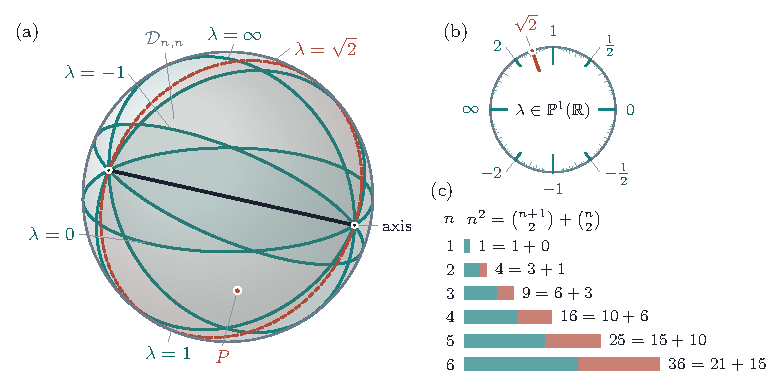
\includegraphics[width=0.80\textwidth]{fig_lagsweep}
\caption{The quaternionic loci of \Cref{prop:lagrangian}, drawn as a
pencil. Each admissible $\psi$ gives one leaf, an open piece of
$\mathrm{LG}(n,V_{+},\omega_{\psi})$ of dimension $n(n+1)/2$. As $\psi$
varies over the reals the leaves through a common axis form a continuous
family and sweep out $\cD_{n,n}$. The two heavy leaves are those with $\psi$
rational, and only such leaves are quaternionic loci of abelian varieties.
The drawing is faithful to the continuity of the family and to the
discreteness of its rational members, but not to dimensions: in the family
the leaves have dimension $n(n+1)/2$ inside $n^{2}$, hence codimension
$n(n-1)/2$, which vanishes only at $n=1$ (at $n=2$ the leaves are divisors,
\Cref{rem:ntwo}), and $\psi$ ranges over a real variety rather than an
interval.}
\label{fig:lagsweep}
\end{figure}

\begin{remark}[Real and rational quaternionic loci]%
\label{rem:onlyrational}
Fix a point $P$ of $\cD_{n,n}$, and let $\psi_{0}$ be left multiplication by
$j$ at a point $P_{0}$ given by \Cref{thm:quatweil}(iii). The group
$\SU(V,H)(\RR)$ acts transitively on the bounded symmetric domain $\cD_{n,n}$
of \Cref{prop:weildomain}, so $P=gP_{0}$ for some real $g$; since $g$ is
$K$-linear and preserves $H$, hence $E$, the map
$\psi=g\psi_{0}g^{-1}$ is $K$-semilinear, invertible and Rosati-symmetric,
satisfies $\psi^{2}=b$, and preserves the Hodge structure at $P$. It
satisfies every condition of \Cref{prop:lagrangian} except rationality, and
$P$ lies on its locus. So the quaternionic loci, taken over the \emph{real}
$\psi$, cover $\cD_{n,n}$; they cover it with room to spare, since each has
dimension $n(n+1)/2$ and they are parametrised by a positive-dimensional
family. What prevents the quaternionic loci of abelian varieties from
covering it is that $\psi$ must lie in $\End^{0}(A)$, hence be rational, and
the rational $\psi$ form a countable set.

This is the dichotomy of \Cref{cor:allornothing} in its simplest form. The
obstruction is the countability of a set of parameters inside an uncountable
one, and it involves neither deformation theory nor positivity. What is
needed is a mechanism that produces, from one rational $\psi$, a family of
cycles representing $\omega$ over an open subset of $\cD_{n,n}$ rather than
over the locus of $\psi$ alone; by \Cref{cor:allornothing}, such a family
would answer \Cref{q:residual} in the affirmative.
\end{remark}

\subsection{Absolutely Hodge classes and the exact form}\label{ssec:exactform}

The algebraicity of a Hodge class is usually approached through an
intermediate property. A rational class of type $(p,p)$ on a smooth
projective variety $X$ over $\CC$ is \emph{absolutely Hodge} if, for every
automorphism $\sigma$ of $\CC$, the conjugate under $\sigma$ of its de Rham
component is the de Rham component of a rational class of type $(p,p)$ on the
conjugate variety $X^{\sigma}$. The implications
\begin{equation}\label{eq:threechain}
  \text{algebraic}
  \;\Longrightarrow\;
  \text{absolutely Hodge}
  \;\Longrightarrow\;
  \text{Hodge}
\end{equation}
are both elementary. The Hodge conjecture asserts the converse of their
composite. The converse of the second is the weaker statement, and Deligne
proved it for abelian varieties, so on abelian varieties the Hodge conjecture
is the converse of the first.

\begin{theorem}[Deligne \cite{Del82}]\label{thm:deligneAH}
Every Hodge class on a complex abelian variety is absolutely Hodge. Moreover,
\emph{Principle B}: if $\pi\colon\cX\to S$ is smooth projective over a
connected smooth base, and $\alpha$ is a flat section of $R^{2p}\pi_{*}\QQ(p)$
that is Hodge at every point of $S$ and absolutely Hodge at one point, then it
is absolutely Hodge at every point.
\end{theorem}

Together with \Cref{thm:residual} and \Cref{thm:everyfamily}, this locates
the remaining problem.

\begin{corollary}[Reduction to an absolutely Hodge class]\label{cor:exactform}
Let $\pi\colon\cA\to\cD_{n,n}$ and $\omega$ be as in \Cref{setup:family}. Then
$\omega_{s}$ is absolutely Hodge for every $s$, and the following are
equivalent:
\begin{enumerate}[label=\textup{(\roman*)},nosep]
\item the Hodge conjecture holds, in every degree, for every abelian
  $2n$-fold of $(K,-1,n)$-Weil type with $\Hg(A)=\SU(V,H)$;
\item the absolutely Hodge class $\omega_{s}$ is algebraic for every $s$.
\end{enumerate}
This holds for every $K$, every $n$ and every discriminant.
\end{corollary}

\begin{proof}
The first assertion is \Cref{thm:deligneAH}. It also follows from Principle B
together with \Cref{thm:everyfamily}, which supplies a point of $\cD_{n,n}$ at
which $\omega$ is algebraic and hence absolutely Hodge, and with the
connectedness of $\cD_{n,n}$ from \Cref{prop:weildomain}.

That (ii) implies (i) is \Cref{thm:residual}(a). Conversely, the Hodge group
of $A_{s}$ is $\SU(V,H)$ for $s$ outside a countable union of proper closed
analytic subsets of $\cD_{n,n}$, by Weil's theorem \cite{Weil77} recalled
before \Cref{thm:hdgcount}. Under (i) the class $\omega_{s}$ is algebraic at
all such $s$, so the set $\Sigma$ of points at which it is algebraic is not
meagre, and \Cref{cor:allornothing} gives $\Sigma=\cD_{n,n}$, which is (ii).
\end{proof}

\section{The algebraic locus and the propagation criteria}\label{sec:propagation}

The results of \Cref{sec:basepoints} are pointwise: a class, a criterion and
a cycle at a point, and in \Cref{cor:exactform} an implication to be proved
at every point. This section studies the set of points at which the Weil class
is algebraic. Properness of the Hilbert scheme makes it a countable union of
closed subvarieties (\Cref{thm:closedlocus}), and rational isogenies make it
dense (\Cref{prop:densealg}); together these turn the propagation question
into a dichotomy (\Cref{cor:allornothing}). Two criteria for propagation
follow, a bound along one orbit (\Cref{thm:degreebound}) and a rank at one
point (\cite[Theorem~2.3]{paperII}). We treat the bound first, together with
the transport of cycles along isogenies, which decides one of its two
readings, and with the limits of representatives built from products of
divisors; the rest of the section is devoted to the rank.

\subsection{The algebraic locus}
\label{ssec:properness}

\Cref{q:residual} is a question about the set
\[
  \Sigma \;=\; \bigl\{\,s\in\cD_{n,n} \;:\;
    \omega_{s}\ \text{is algebraic on}\ A_{s}\,\bigr\}.
\]
This set is restricted in shape, and the restriction changes the form
of the remaining problem: instead of a class to construct at every point, one
is left with a bound to prove along one orbit, or a rank to compute at one
point. The reason is that the Hilbert scheme is proper, so each piece of
$\Sigma$ cut out by bounded data is Zariski closed. The mechanism is standard:
the locus where a fixed Hodge class becomes algebraic is a countable union of
closed subvarieties, the companion of the statement that the Hodge locus
itself is one (see \cite[Chapter~5]{Voi03} and, in the form used in
\Cref{thm:cdk}, \cite{CDK95}). What is particular to the present situation is
that the class is determined by \Cref{thm:hdgcount} and written out by
\Cref{thm:explicitgens}, that its algebraic locus is nonempty in every family
by \Cref{thm:everyfamily}, and that the group acting on the family is known.

\begin{setupenv}[The quotient and the universal family]\label{setup:shimura}
Keep \Cref{setup:family}. Fix an integer $N\ge3$ and let $\Gamma$ be the
subgroup of $\SU(V,H)(\QQ)$ preserving the lattice $L\subset V$ used to build
the family and acting trivially on $L/NL$. Write
\[
  p\colon\cD_{n,n}\longrightarrow\cS=\Gamma\backslash\cD_{n,n} .
\]
Since $N\ge3$ the group $\Gamma$ is torsion-free, so it acts freely on
$\cD_{n,n}$, and by Baily and Borel \cite{BB66} the quotient $\cS$ is a smooth
quasi-projective complex variety; it is irreducible because $\cD_{n,n}$ is
connected. The level structure rigidifies, so $\cS$ carries a universal family
\[
  f\colon\cA\longrightarrow\cS,
\]
and the relative polarisation $3\eta$ is relatively very ample, which fixes a
relative projective embedding and hence a notion of degree in the fibres.
Write $G=\SU(V,H)$, an algebraic group over $\QQ$, so that
$G(\RR)$ acts transitively on $\cD_{n,n}$ and $\Gamma\subset G(\QQ)$.
\end{setupenv}

We record two facts that are used repeatedly below.

\begin{lemma}[The section descends]\label{lem:omegadescends}
The section $\omega$ of \Cref{setup:family} is $\Gamma$-invariant, hence
descends to a flat section of $R^{2n}f_{*}\QQ$ over $\cS$ that is of type
$(n,n)$ at every point.
\end{lemma}

\begin{proof}
The Weil line is $\HW=\bigwedge^{2n}_{K}V$, and an element of $\SU(V,H)$ is by
definition a $K$-linear automorphism of $V$ of $K$-determinant $1$. Its action
on the top $K$-exterior power is multiplication by that determinant, so
$\Gamma$ acts trivially on $\HW$ and in particular fixes $\omega$. Flatness is
then immediate, and the Hodge type at every point is
\Cref{prop:weilline}(ii).
\end{proof}

\begin{lemma}[One component is enough]\label{lem:onecomponent}
Let $(A,\iota,\eta)$ be of $(K,-1,n)$-Weil type with
$\iota(\cO_{K})\subseteq\End(A)$, and let $\HW\subset H^{2n}(A,\QQ)$ be its
Weil line. If one nonzero element of $\HW$ is algebraic, every element of
$\HW$ is algebraic.
\end{lemma}

\begin{proof}
Among the elements $\tau_{m}=m+\sqrt{-d}$ of $\cO_{K}$ with $1\le m\le7$ the
ratios $\tau_{m}/\bbar{\tau}_{m}$ are pairwise distinct, since
$\tau_{m}\bbar{\tau}_{m'}$ is rational only when $m=m'$. The group of roots of
unity in an imaginary quadratic field has order $2$, $4$ or $6$, so some $m$
in that range has $\tau=\tau_{m}$ with $\tau/\bbar\tau$ not a root of unity,
and then $\tau^{2n}\ne\bbar{\tau}^{2n}$, that is $\tau^{2n}\notin\QQ$, for
every $n\ge1$. A range is needed, since the witness $m=1$ fails for two
fields: for $d=1$ the ratio attached to $1+\sqrt{-1}$ is a primitive fourth
root of unity, and for $d=3$ the ratio attached to $1+\sqrt{-3}$ is a
primitive cube root of unity, so $(1+\sqrt{-d})^{2n}$ is rational when $d=1$
and $n$ is even, and when $d=3$ and $3\mid n$.

Since $\tau\in\cO_{K}$, the element $\iota(\tau)$ is an endomorphism of $A$,
so $\iota(\tau)^{*}$ on $H^{2n}(A,\QQ)$ is induced by the graph
correspondence and therefore carries algebraic classes to algebraic classes.
On $H^{1}$ it is multiplication by $\tau$, so on
$\bigwedge^{2n}_{K}V$ it is multiplication by $\tau^{2n}$. As
$\tau^{2n}\notin\QQ$ and $\HW$ is a one-dimensional $K$-vector space, the pair
$w,\;\tau^{2n}w$ is a $\QQ$-basis of $\HW$ for every $w\ne0$. Explicitly, fix
a $K$-basis $w_{0}$ of $\HW$ and write $\tau^{2n}=a+b\sqrt{-d}$, so that
$b\ne0$, and $w=(w_{1}+w_{2}\sqrt{-d})\,w_{0}$; the determinant of the pair
$w,\tau^{2n}w$ in the $\QQ$-basis $w_{0},\sqrt{-d}\,w_{0}$ is
$b(w_{1}^{2}+dw_{2}^{2})$, which is nonzero when $w\ne0$. If $w$ is
algebraic then so is $\iota(\tau)^{*}w=\tau^{2n}w$, and the two together span.
\end{proof}

\Cref{lem:onecomponent} writes out the last step of the proof of
\Cref{cor:whatisleft}, where the witness $\tau$ has to be chosen.

\begin{theorem}[The algebraic locus is a countable union of closed
subvarieties]\label{thm:closedlocus}
Keep \Cref{setup:shimura}. For a finite tuple $\underline{P}=(P_{1},\dots
,P_{m})$ of Hilbert polynomials of degree $n$ and a tuple
$\underline{q}\in\QQ^{m}$ put
\begin{align*}
  \cH_{\underline{P}}
  &\;=\;
  \Hilb^{P_{1}}(\cA/\cS)\times_{\cS}\cdots\times_{\cS}\Hilb^{P_{m}}(\cA/\cS),
  \\[2pt]
  \Sigma_{\underline{P},\underline{q}}
  &\;=\;
  \mathrm{pr}\Bigl(\bigl\{\,\underline{Z}\in\cH_{\underline{P}}
    \;:\;\textstyle\sum_{i}q_{i}[Z_{i}]=\omega\,\bigr\}\Bigr)
  \;\subseteq\;\cS .
\end{align*}
Then each $\Sigma_{\underline{P},\underline{q}}$ is Zariski closed in
$\cS$, and
\[
  p^{-1}\Bigl(\,\bigcup_{\underline{P},\underline{q}}
    \Sigma_{\underline{P},\underline{q}}\Bigr)\;=\;\Sigma ,
\]
the union running over a countable index set.
\end{theorem}

\begin{proof}
Each $\Hilb^{P_{i}}(\cA/\cS)$ is projective over $\cS$ by Grothendieck's
construction of the Hilbert scheme \cite{Gro61}, so the fibre product
$\cH_{\underline{P}}$ is
projective over $\cS$, and being of finite type it has finitely many connected
components.

Fix a connected component $T$, replace it by its reduction, which changes
neither the underlying space nor any cohomology group, and let
$\cZ_{i}\subset\cA\times_{\cS}T$ be the pullback of the $i$-th universal
subscheme. It is flat over $T$ and its fibres have Hilbert polynomial $P_{i}$
of degree $n$, so the associated $n$-cycles, the top-dimensional components
counted with their multiplicities, are the fibres of a cycle on
$\cA\times_{\cS}T$ whose class restricts on the fibre over $t$ to $[Z_{i,t}]$.
Restriction of a global class to the fibres of a topologically
locally trivial family is a flat section of the local system, so
$t\mapsto\sum_{i}q_{i}[Z_{i,t}]$ is flat on $T$; and $\omega$ is flat on $\cS$
by \Cref{lem:omegadescends}, hence flat after pullback. Two flat sections of a
local system over a connected base agree everywhere as soon as they agree at
one point, so the locus where they agree is a union of connected components of
$\cH_{\underline{P}}$. That locus is therefore itself projective over $\cS$,
and the image of a proper morphism is Zariski closed.

For the equality of sets, let $s\in\Sigma$. Then
$\omega_{s}=\sum_{i}q_{i}[Z_{i}]$ for finitely many closed integral subschemes
$Z_{i}\subset A_{s}$ of dimension $n$ and rationals $q_{i}$; taking
$P_{i}$ to be the Hilbert polynomial of $Z_{i}$ puts $p(s)$ in
$\Sigma_{\underline{P},\underline{q}}$. The converse holds because the class
of the $n$-cycle of a closed subscheme of dimension $n$ is algebraic. The
index set is countable, since a Hilbert polynomial is determined by its
finitely many integer coordinates in the binomial basis, and $\QQ$ is
countable.
\end{proof}

The bound on the Hilbert polynomials cannot be dropped: without it one takes
the image of an infinite disjoint union, and an infinite union of closed sets
need be neither closed nor constructible, and the dichotomy below is what
can be said of $\Sigma$ itself. Tuples are needed because a rational cycle is a rational combination
of several integral ones, which may have different Hilbert polynomials. The
relative Chow variety of effective $n$-cycles of bounded degree would serve
equally well, with the same proof, since only properness over the base and
local constancy of the cycle class are used.

\begin{corollary}[The dichotomy]\label{cor:allornothing}
Exactly one of the following holds.
\begin{enumerate}[label=\textup{(\alph*)},nosep]
\item $\Sigma=\cD_{n,n}$, and the Hodge conjecture holds in every degree for
  every abelian $2n$-fold of $(K,-1,n)$-Weil type with $\Hg(A)=\SU(V,H)$ in
  the family.
\item $\Sigma$ has empty interior in the analytic topology. Its complement is
  then a dense $G_{\delta}$, so $\omega_{s}$ fails to be algebraic for every
  $s$ outside a meagre set, and the Hodge conjecture fails.
\end{enumerate}
In particular, if $\omega_{s}$ is algebraic for all $s$ in some nonempty open
subset of $\cD_{n,n}$, then it is algebraic for all $s$.
\end{corollary}

\begin{proof}
Suppose $\Sigma$ contains a nonempty open set; then so does its image in
$\cS$, and we may pick a nonempty connected open $U\subseteq\cS$ contained in
that image. By \Cref{thm:closedlocus} the countably many sets
$\Sigma_{\underline{P},\underline{q}}\cap U$ are closed in $U$ and cover it.
A connected complex manifold is a Baire space, so one of them has nonempty
interior in $U$. A Zariski closed subset of the irreducible variety $\cS$
either is all of $\cS$ or is a proper closed subvariety, and a proper closed
subvariety of a connected complex manifold has empty interior. Hence that
$\Sigma_{\underline{P},\underline{q}}$ is all of $\cS$, so $\Sigma=\cD_{n,n}$
and (a) holds by \Cref{thm:residual}(a). If $\Sigma$ has empty interior, its
complement is the intersection of the countably many dense open sets
$\cD_{n,n}\setminus p^{-1}(\Sigma_{\underline{P},\underline{q}})$, and Baire
again gives that this intersection is dense. At each of its points
$\omega_{s}$ is a Hodge class by \Cref{lem:omegadescends} and is not
algebraic, so the Hodge conjecture fails there.
\end{proof}

\Cref{fig:properness} draws the two cases.

\begin{figure}[htbp]
\centering
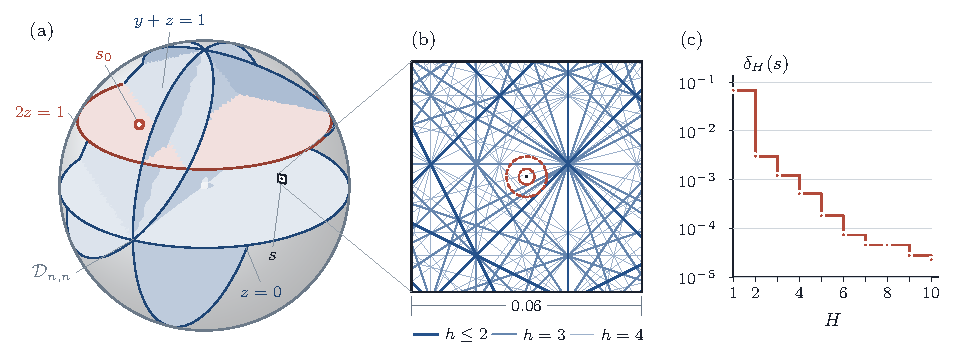
\includegraphics[width=0.88\textwidth]{fig_properness}
\caption{The dichotomy of \Cref{cor:allornothing}. Each stratum
$\Sigma_{\underline{P},\underline{q}}$ is Zariski closed by
\Cref{thm:closedlocus}, and there are countably many of them; the base point
$s_{0}$ of \Cref{thm:everyfamily} lies on one. By \Cref{prop:densealg} the
union of the strata is dense, so every neighbourhood of a point $s$ lying
off all of them meets infinitely many strata. The conjecture for the family
is the assertion that no such $s$ exists, and by \Cref{cor:allornothing} it
is enough that one stratum has nonempty interior.}
\label{fig:properness}
\end{figure}

\begin{lemma}[Invariance under rational isogenies]\label{lem:Ginvariance}
$\Sigma$ is stable under the action of $G(\QQ)$ on $\cD_{n,n}$.
\end{lemma}

\begin{proof}
A point of $\cD_{n,n}$ is a complex structure $J$ on $V_{\RR}$ compatible with
$H$, and $g\in G(\QQ)$ carries $J$ to $gJg^{-1}$. The map $g$ is then
$\QQ$-rational and $\CC$-linear from $(V_{\RR},J)$ to $(V_{\RR},gJg^{-1})$, so
after clearing denominators it induces an isogeny $A_{J}\to A_{gJ}$, whose
graph is an algebraic correspondence. Algebraicity of a rational cohomology
class is preserved by such a correspondence and by its transpose. Finally $g$
lies in $\SU(V,H)$, so by the computation in \Cref{lem:omegadescends} it fixes
the Weil line pointwise; the correspondence therefore carries $\omega_{J}$ to
a nonzero rational multiple of $\omega_{gJ}$, and $\omega_{gJ}$ is algebraic
when $\omega_{J}$ is.
\end{proof}

Two density statements should be distinguished. For a class that does not
remain of Hodge type over the whole family, the locus where it is of Hodge
type is a countable union of proper closed subvarieties, each algebraic by
\Cref{thm:cdk}, and density there concerns the distribution of special
points. For the class $\omega$ of \Cref{setup:family} the Hodge locus is the
whole family by \Cref{prop:weilline}(ii), so \Cref{thm:cdk} gives no
information, and the set that carries information is the algebraic locus. The
next proposition concerns that set, and its proof uses no Hodge theory: the
algebraic locus is a union of orbits of a group whose rational points are
dense in its real points.

\begin{proposition}[The algebraic locus is dense]\label{prop:densealg}
Let $n\ge2$. Then $\Sigma$ is dense in $\cD_{n,n}$ in the analytic topology,
and its image in $\cS$ is dense.
\end{proposition}

\begin{proof}
The hermitian form $H$ has rank $2n\ge4$ over $K$ and signature $(n,n)$, so it
is isotropic over $\RR$; over every $\QQ_{p}$ a hermitian form of rank at
least three over a quadratic extension is isotropic; and hermitian forms over
an imaginary quadratic field satisfy the Hasse principle
\cite[Ch.~10, \S 6]{Sch85}. So $H$ is isotropic over $\QQ$ and $G$ is
$\QQ$-isotropic. The group $G=\SU(V,H)$ is simply connected and almost
$\QQ$-simple, so by Platonov's theorem $G(\QQ)$ is generated by the rational
points of the unipotent radicals of its proper parabolic $\QQ$-subgroups
\cite[Thm.~7.6 and \S 7.2]{PR94}. For a unipotent group $U$ over $\QQ$ the
exponential identifies $U(\QQ)$ with a $\QQ$-vector space inside the
corresponding $\RR$-vector space $U(\RR)$, so $U(\QQ)$ is dense in $U(\RR)$.
The closure of $G(\QQ)$ in $G(\RR)$ therefore contains $U(\RR)$ for every such
$U$, and those generate the identity component $G(\RR)^{+}$, which acts
transitively on $\cD_{n,n}$. Hence every $G(\QQ)$-orbit in $\cD_{n,n}$ is
dense.

By \Cref{thm:everyfamily} the set $\Sigma$ is nonempty, and by
\Cref{lem:Ginvariance} it is $G(\QQ)$-stable, so it contains a dense orbit.
The projection $p$ is continuous and surjective, so the image is dense.
\end{proof}

In particular, if case (b) of \Cref{cor:allornothing} occurs, then $\Sigma$
and its complement are both dense, and the two sets are distinguished by
Baire category and not by position.

\begin{corollary}[A Baire category criterion]\label{cor:meagre}
Let $n\ge2$. The Hodge conjecture holds for every abelian $2n$-fold of
$(K,-1,n)$-Weil type with $\Hg(A)=\SU(V,H)$ in the family of
\Cref{setup:family} if and only if $\Sigma$ is non-meagre in $\cD_{n,n}$, and
if and only if $\Sigma$ has nonempty interior.
\end{corollary}

\begin{proof}
If $\Sigma=\cD_{n,n}$, both conditions hold, and so does the conjecture, by
\Cref{thm:residual}(a). Otherwise case (b) of \Cref{cor:allornothing} holds,
so $\Sigma$ has empty interior; it is then the countable union of the closed
sets $p^{-1}(\Sigma_{\underline{P},\underline{q}})$, each with empty interior,
and so it is meagre. The points $s$ with $\Hg(A_{s})=\SU(V,H)$ form the
complement of a countable union of proper closed analytic subsets of $\cD_{n,n}$, by
Weil's theorem \cite{Weil77} recalled before \Cref{thm:hdgcount}, so by Baire
they are not all contained in the meagre set $\Sigma$. At a point of this
kind outside $\Sigma$ the Hodge conjecture fails for $A_{s}$.
\end{proof}

\subsection{The first criterion: a bound along one orbit}

The proof of \Cref{prop:densealg} produces the dense algebraic locus by
transporting one cycle along rational isogenies, and an isogeny multiplies
degrees. The dense set so obtained is therefore stratified by unbounded data,
and this is what prevents \Cref{cor:allornothing} from applying to it. A bound
on the data along one orbit removes the difficulty.

\begin{theorem}[A bound along the orbit closes the family]\label{thm:degreebound}
Let $n\ge2$ and let $s_{0}\in\Sigma$ be one of the base points supplied by
\Cref{thm:everyfamily}. Suppose that there is a finite set $\mathcal{T}$ of pairs
$(\underline{P},\underline{q})$ such that for every $g\in G(\QQ)$ the class
$\omega_{g\cdot s_{0}}$ is represented by some cycle whose Hilbert data lies
in $\mathcal{T}$. Then $\Sigma=\cD_{n,n}$, and the Hodge conjecture holds in every
degree for every abelian $2n$-fold of $(K,-1,n)$-Weil type with
$\Hg(A)=\SU(V,H)$ in that family.
\end{theorem}

\begin{proof}
The orbit $G(\QQ)\cdot s_{0}$ is dense by the proof of \Cref{prop:densealg},
and by hypothesis it is the union of the finitely many sets
$G(\QQ)\cdot s_{0}\cap p^{-1}(\Sigma_{\underline{P},\underline{q}})$ with
$(\underline{P},\underline{q})\in\mathcal{T}$. The union of the finitely
many closed sets $p^{-1}(\Sigma_{\underline{P},\underline{q}})$,
$(\underline{P},\underline{q})\in\mathcal{T}$, therefore contains a dense set,
and so it is all of $\cD_{n,n}$; in particular $\Sigma=\cD_{n,n}$. In fact one
of these sets is already all of $\cS$: each
$\Sigma_{\underline{P},\underline{q}}$ is Zariski closed in the irreducible
variety $\cS$, hence either equal to $\cS$ or nowhere dense, and a finite
union of nowhere dense sets is nowhere dense. The Hodge conjecture for the
family follows by \Cref{thm:residual}(a).
\end{proof}

\begin{remark}[Choice of the representing cycle]\label{rem:chosencycle}
We call the hypothesis of \Cref{thm:degreebound} the bounded criterion
\textup{(P1)}; \cite[Remark~3.7]{paperII} lists it beside the rank criterion
\textup{(P2)} of \cite[Theorem~2.3]{paperII}. It quantifies over representing
cycles at each point of the orbit and asks only that, at each point, one of
them have bounded complexity. A stronger hypothesis would fix the cycle,
taking at $g\cdot s_{0}$ the transport of the cycle at $s_{0}$ along the
isogeny of \Cref{lem:Ginvariance}. \Cref{thm:p1forces} below shows that this
stronger form is never satisfied by a base cycle with a component of finite
stabiliser, since the transported data is then unbounded. The proof above
uses only the weaker hypothesis, which is what the covering argument needs.
\end{remark}

The hypothesis of \Cref{thm:degreebound} can be sharpened by locating the
part of the Hilbert data that is at issue. The leading coefficient is not.

\begin{proposition}[The leading coefficient is constant on the orbit]
\label{prop:leadingconstant}
Let $s_{0}\in\Sigma$ and $g\in G(\QQ)$, and let $\omega_{s}$ denote the Weil
class at $s$ and $\eta$ the polarisation class. Then
\[
  \int_{A_{g\cdot s_{0}}}\omega_{g\cdot s_{0}}\cdot\frac{\eta^{n}}{n!}
  \;=\;\int_{A_{s_{0}}}\omega_{s_{0}}\cdot\frac{\eta^{n}}{n!},
\]
so the degree of the transported class with respect to the polarisation, which
is the leading coefficient of the Hilbert polynomial of any cycle
representing it, is the same at every point of the orbit.
\end{proposition}

\begin{proof}
By \Cref{lem:Ginvariance} the correspondence transporting the class is induced
by a $\QQ$-rational map $g\in\SU(V,H)$. It preserves the hermitian form and
hence the polarisation class, it fixes the Weil line pointwise by
\Cref{lem:omegadescends}, and its determinant over $\QQ$ is
$\Nm_{K/\QQ}(\det_{K}g)=1$, so it acts trivially on the top exterior power of
$V^{\vee}$, in which both integrals are evaluated. The two integrals are
therefore equal. The identification of the number with the leading
coefficient is Hirzebruch--Riemann--Roch on $A$, whose Todd class is $1$ (for
the embedding by $3\eta$ of \Cref{setup:shimura} the leading coefficient is
$3^{n}$ times the number); the remaining coefficients involve the structure
sheaf of the cycle and not only its class.
\end{proof}

\begin{remark}[The source of unboundedness]
\label{rem:whereunbounded}
Write a representing cycle at a point of the orbit, the transported cycle or
any other, as a difference $\xi^{+}-\xi^{-}$ of effective cycles. By
\Cref{prop:leadingconstant} the difference of their degrees is constant along
the orbit, and by the boundedness of effective cycles of bounded degree in
the fibres of the polarised family $f\colon\cA\to\cS$, if $\deg\xi^{+}$ were
bounded along the orbit then only finitely many tuples
$(\underline{P},\underline{q})$ could occur and \Cref{thm:degreebound} would
apply. So the hypothesis of that theorem is equivalent to a bound on the
effective part alone.

This bound is not automatic, and the mechanism that threatens it can be seen
directly. The transport at $g$ is by the isogeny obtained from $g$ by
clearing denominators; if $g$ has denominator $m$ on the reference lattice,
which has rank $4n$, the isogeny has degree $m^{4n}$ (\Cref{lem:transport}
below), and pushing a cycle forward along it multiplies its multiplicities
and degrees by powers of $m$ (\Cref{lem:multiplicity}). Elements of $G(\QQ)$ of bounded denominator form a discrete subset of
$G(\RR)$, so along a dense orbit the denominators, and with them the isogeny
degrees, are unbounded. What \Cref{thm:degreebound} asks is that the cycles
nevertheless simplify: that at each point of the orbit the class $\omega$,
whose degree has not changed, admits an effective representation no more
complicated than before. For the transported cycle itself the answer is
negative as soon as a component of the base cycle has finite stabiliser
(\Cref{thm:p1forces} below), and for a cycle chosen at each point the bound
is equivalent to the conclusion (\Cref{thm:p1equivalent}). The present remark
shows only that the question reduces from the whole Hilbert datum to the
degree of the effective part, and that the part of the datum determined by
cohomology is constant.
\end{remark}

\subsection{Transport along isogenies}

The mechanism of \Cref{rem:whereunbounded} can be made explicit, and doing
so settles one of the two readings of \textup{(P1)}: the reading in
which the cycle at $s_{0}$ is transported along the orbit rather than chosen
afresh at each point. Write $\Lambda$ for the reference lattice, of rank $4n$
over $\ZZ$, and $E$ for the alternating form of the polarisation, so that a
point $s$ of $\cD_{n,n}$ is a complex structure on $\Lambda\otimes\RR$ and
$A_{s}=(\Lambda\otimes\RR)/\Lambda$. Throughout, $\dim A_{s}=2n$, and a
component of a cycle representing $\omega_{s}$ has dimension $n$.

\begin{lemma}[The transport in coordinates]\label{lem:transport}
Let $g\in G(\QQ)$ and let $c=c(g)$ be the least positive integer with
$cg\Lambda\subseteq\Lambda$. Then $\varphi_{g}:=cg$ induces an isogeny
$A_{s_{0}}\to A_{g\cdot s_{0}}$ with
\begin{enumerate}[label=\textup{(\roman*)},nosep,leftmargin=2.6em]
\item $\deg\varphi_{g}=c^{4n}$;
\item $\varphi_{g}^{*}\eta_{g\cdot s_{0}}=c^{2}\eta_{s_{0}}$ and
  $\varphi_{g}^{*}\omega_{g\cdot s_{0}}=c^{2n}\omega_{s_{0}}$;
\item the transported cycle representing $\omega_{g\cdot s_{0}}$ is
  $c^{-2n}\,\varphi_{g*}(Z)$, where $Z$ represents $\omega_{s_{0}}$.
\end{enumerate}
Moreover $\sup_{g\in G(\QQ)}c(g)=\infty$.
\end{lemma}

\begin{proof}
(i) The index of $cg\Lambda$ in $\Lambda$ is $|\det_{\QQ}(cg)|
=c^{4n}|\det_{\QQ}g|$, and $\det_{\QQ}g=\Nm_{K/\QQ}(\det_{K}g)=1$ for
$g\in\SU(V,H)$.

(ii) $g$ preserves $E$, so $(cg)^{*}E=c^{2}E$, which is the first identity.
On $H^{2n}=\bigwedge^{2n}(\Lambda^{\vee}\otimes\QQ)$ the map
$\varphi_{g}^{*}$ is $c^{2n}\bigwedge^{2n}g^{\vee}$, and $g\in\SU(V,H)$ fixes
the Weil line pointwise by \Cref{lem:omegadescends}.

(iii) $\varphi_{g*}\varphi_{g}^{*}=\deg\varphi_{g}$, so
$\omega_{g\cdot s_{0}}=(\deg\varphi_{g})^{-1}\varphi_{g*}
\varphi_{g}^{*}\omega_{g\cdot s_{0}}
=c^{-4n}\,c^{2n}\varphi_{g*}\omega_{s_{0}}=c^{-2n}\varphi_{g*}\omega_{s_{0}}$
by (i) and (ii).

For the last sentence, suppose that $c(g)\le C$ for every $g\in G(\QQ)$.
Then $(C!)\,g\Lambda\subseteq\Lambda$ for every $g$, so $G(\QQ)$ lies in the
discrete subset $(C!)^{-1}\End_{\ZZ}(\Lambda)$ of $\End(\Lambda\otimes\RR)$.
But by the proof of \Cref{prop:densealg} the closure of $G(\QQ)$ in $G(\RR)$
contains $G(\RR)^{+}$, a Lie group of positive dimension, which is a
contradiction.
\end{proof}

\begin{lemma}[Push-forward along an isogeny]
\label{lem:multiplicity}
Let $\varphi\colon A\to A'$ be an isogeny of abelian varieties and $Z\subseteq A$
an integral closed subvariety. Put
$G(Z)=\{x\in A:Z+x=Z\}$, a closed algebraic subgroup. Then
\[
  \varphi_{*}[Z]=m\,[\varphi(Z)],\qquad
  m=\bigl|\ker\varphi\cap G(Z)\bigr| .
\]
If moreover $\dim Z=n$ and $\varphi^{*}\eta'=c^{2}\eta$, then
\[
  \deg_{\eta'}\varphi(Z)=\frac{c^{2n}}{m}\,\deg_{\eta}Z .
\]
\end{lemma}

\begin{proof}
The map $\varphi|_{Z}\colon Z\to\varphi(Z)$ is finite and surjective, and its
degree $m$ is the number of points of a general fibre. For $z\in Z$ the fibre
through $z$ is $Z\cap(z+\ker\varphi)$, which as a set of translations is
$\{t\in\ker\varphi:z+t\in Z\}$. For a fixed $t$ the locus
$\{z\in Z:z+t\in Z\}=Z\cap(Z-t)$ is all of $Z$ when $t\in G(Z)$ and a proper
closed subset otherwise; since $\ker\varphi$ is finite, a general $z$ avoids
the finitely many proper subsets, and there
$\{t\in\ker\varphi:z+t\in Z\}=\ker\varphi\cap G(Z)$. This is the first
identity, and $\varphi_{*}[Z]=m[\varphi(Z)]$ by the definition of the
push-forward of cycles.

For the degree, the projection formula gives
\[
  m\deg_{\eta'}\varphi(Z)=\int\varphi_{*}[Z]\cdot\frac{\eta'^{n}}{n!}
  =\int[Z]\cdot\frac{(\varphi^{*}\eta')^{n}}{n!}
  =c^{2n}\int[Z]\cdot\frac{\eta^{n}}{n!}=c^{2n}\deg_{\eta}Z .
\]
\end{proof}

For example, for multiplication by $c$ on an abelian variety of dimension $2n$,
an abelian subvariety $Z$ of dimension $n$ has $G(Z)=Z$, so $m=|Z[c]|=c^{2n}$
and $\deg\varphi(Z)=\deg Z$, while a $Z$ whose stabiliser meets $A[c]$
trivially has $m=1$ and $\deg\varphi(Z)=c^{2n}\deg Z$.

\begin{theorem}[The transported cycle]\label{thm:p1forces}
Let $s_{0}\in\Sigma$ and let $Z=\sum_{i}q_{i}Z_{i}$, with $q_{i}\ne0$ and the
$Z_{i}$ integral of dimension $n$, represent $\omega_{s_{0}}$.
\begin{enumerate}[label=\textup{(\roman*)},leftmargin=2.6em,itemsep=2pt]
\item For $g\in G(\QQ)$ the transported cycle is
  $\sum_{i}c(g)^{-2n}m_{i}(g)\,q_{i}\,[\varphi_{g}(Z_{i})]$ with
  $m_{i}(g)=|\ker\varphi_{g}\cap G(Z_{i})|$, and the $i$-th component has
  degree $c(g)^{2n}\deg_{\eta}(Z_{i})/m_{i}(g)$.
\item If some $Z_{i}$ has finite stabiliser $G(Z_{i})$, then
  $\deg\varphi_{g}(Z_{i})\ge c(g)^{2n}\deg_{\eta}(Z_{i})/|G(Z_{i})|$, which is
  unbounded on $G(\QQ)$. The Hilbert data of the transported cycle then takes
  infinitely many values, and the hypothesis of \Cref{thm:degreebound} in the
  form that fixes the transported cycle is not satisfied by $Z$.
\item Consequently, a base cycle for which the transported data is bounded
  must have every component of positive-dimensional stabiliser, that is, every
  $Z_{i}$ must be stable under translation by a positive-dimensional abelian
  subvariety of $A_{s_{0}}$.
\end{enumerate}
\end{theorem}

\begin{proof}
(i) is \Cref{lem:transport}(iii) and \Cref{lem:multiplicity}.

(ii) $\ker\varphi_{g}\cap G(Z_{i})\subseteq G(Z_{i})$, so
$m_{i}(g)\le|G(Z_{i})|$, a constant; the displayed bound is (i), and $c(g)$ is
unbounded by \Cref{lem:transport}. Distinct degrees of the components give
distinct Hilbert polynomials, so the data takes infinitely many values.

(iii) is the contrapositive of (ii), together with the fact that an algebraic
subgroup of positive dimension in an abelian variety has an abelian subvariety
of positive dimension as its identity component.
\end{proof}

\begin{remark}[The two readings of \textup{(P1)}]\label{rem:p1meaning}
Three points should be kept apart.

First, \textup{(P1)} has two readings, and \Cref{thm:p1forces} settles one of
them. Read with the cycle fixed at $s_{0}$ and transported, it fails for every
base cycle written down in this paper: those cycles are intersections of
divisors, and an intersection of $n$ divisors on an abelian $2n$-fold has
finite stabiliser unless the divisors are pulled back from a quotient, which
the ones here are not. Read with the cycle chosen afresh at each point of the
orbit, which is the form of the hypothesis of \Cref{thm:degreebound}, it is
not affected by \Cref{thm:p1forces}.

Second, the difference between the two readings is the content of
\Cref{lem:multiplicity}. The class $\omega_{g\cdot s_{0}}$ has constant degree
along the orbit, by \Cref{prop:leadingconstant}; what grows is the complexity
of the particular representative that the transport produces, because the
isogeny spreads each component out by the factor $c^{2n}/m_{i}$. When a
component of the base cycle has finite stabiliser, the transport does not
produce a representative of bounded complexity, whether or not one exists.

Third, an approach to \textup{(P1)} must either produce a base cycle supported
on subvarieties with positive-dimensional stabiliser, a strong requirement for
a Weil class, or abandon the transport and bound instead the minimal
complexity of a representative, which is a statement about the Chow variety of
the family and not about any one cycle. Neither is achieved here.
\end{remark}

The bound on the minimal complexity of a representative is the hypothesis of
\Cref{thm:degreebound}, and it is the weakest hypothesis under which the
covering argument runs. The next theorem shows that it is equivalent to the
conclusion. Write $\mathbf{W}(K,n,\delta)$ for the statement that every
abelian $2n$-fold of $(K,-1,n)$-Weil type with discriminant $\delta$
(\Cref{def:disc}) has algebraic Weil classes, $\delta$ being the discriminant
of the family of \Cref{setup:family}.

\begin{theorem}[Equivalence of the bounded criterion]\label{thm:p1equivalent}
Let $n\ge2$, let $s_{0}\in\Sigma$ and keep \Cref{setup:family}. The following
are equivalent.
\begin{enumerate}[label=\textup{(\alph*)},leftmargin=2.6em,itemsep=2pt]
\item There is a finite set $\mathcal{T}$ of pairs
  $(\underline{P},\underline{q})$ such that at every point of the orbit
  $G(\QQ)\cdot s_{0}$ the class $\omega$ is represented by a cycle whose
  Hilbert data lies in $\mathcal{T}$; that is, \textup{(P1)} holds at
  $s_{0}$.
\item There is a single pair $(\underline{P},\underline{q})$ such that at
  every point of $\cD_{n,n}$, not merely of the orbit, the class $\omega$ is
  represented by a cycle with that datum.
\item $\Sigma=\cD_{n,n}$.
\item $\mathbf{W}(K,n,\delta)$ holds, that is, the Weil classes are algebraic
  on every member of the family.
\end{enumerate}
In particular \Cref{thm:degreebound} is an equivalence, and \textup{(P1)} is a
reformulation of the conjecture for the family and not a reduction of it. The
same holds for every CM field, with \Cref{thm:cmpropagation}(iv) in place of
\Cref{thm:degreebound}.
\end{theorem}

\begin{proof}
(a) implies (c) is \Cref{thm:degreebound}. (b) implies (a) is immediate, the
orbit being contained in $\cD_{n,n}$ and $\mathcal{T}$ being the one pair.
(d) implies (c) trivially, and (c) implies (d) because the algebraicity of
$\omega_{s}$ makes the whole Weil line of $A_{s}$ algebraic, by the argument
of \Cref{cor:whatisleft}, written out in \Cref{lem:onecomponent}.

It remains to deduce (b) from (c). If $\Sigma=\cD_{n,n}$ then $\Sigma$ has
nonempty interior, and the proof of \Cref{cor:allornothing} shows that some
$\Sigma_{\underline{P},\underline{q}}$ is then all of $\cS$: the countably
many sets $\Sigma_{\underline{P},\underline{q}}\cap U$ are closed in a
nonempty connected open $U\subseteq\cS$ and cover it, so by Baire one of them
has nonempty interior in $U$, and a proper Zariski closed subvariety of the
irreducible variety $\cS$ has empty interior. By the definition of
$\Sigma_{\underline{P},\underline{q}}$ in \Cref{thm:closedlocus} as the image of a proper morphism, every $s\in\cS$
then carries a tuple $\underline{Z}$ of subschemes with Hilbert polynomials
$\underline{P}$ and $\sum_{i}q_{i}[Z_{i}]=\omega$, which is (b).

For a CM field the same argument applies without change, using
\Cref{thm:cmpropagation}(iii) in place of \Cref{thm:closedlocus} and
\Cref{cor:allornothing}.
\end{proof}

\begin{remark}[Status of the first criterion]\label{rem:p1collapse}
By \Cref{thm:p1equivalent}, \textup{(P1)} is a restatement of the conjecture
for the family and not a route to it. \Cref{thm:degreebound} is a valid
implication, and its covering argument is the only place in the paper where
density of the rational orbit is converted into a global statement; but the
implication has a converse, so verifying its hypothesis for a family is as
hard as proving the conclusion for that family. The boundedness is
nevertheless a concrete finiteness statement about the Chow variety of the
universal family, and a reformulation of $\mathbf{W}(K,n,\delta)$ that
mentions neither Hodge theory nor deformation theory.

The two propagation criteria are therefore not on the same footing. The rank
criterion \textup{(P2)} of \cite[Theorem~2.3]{paperII} is a sufficient
condition with no evident converse: injectivity of one semiregularity map at
one point implies the conjecture for the whole family, while
$\Sigma=\cD_{n,n}$ carries no information about the deformation theory of any
particular perfect complex. In its pure form, with Chern character a Weil
class, it is never satisfied (\cite[Theorem~3.5]{paperII}); the polarised criterion
\textup{(P2$'$)} of \cite[Remark~3.6]{paperII}, in which the Chern character may also
carry powers of the polarisation, is the form studied in
\cite[Section~3]{paperII}.
\end{remark}

\subsection{Products of divisors}

The intersection numbers needed below are Pfaffians. Let $E$ be a
nondegenerate alternating form on a real vector space $V$ of dimension $2g$,
let $\eta$ be its class, with the orientation for which
$e=\int\eta^{g}>0$, and for an $E$-self-adjoint endomorphism $\phi$ write
$x_{\phi}(u,v)=E(\phi u,v)$, an alternating form.

\begin{lemma}[Pfaffians of self-adjoint classes]\label{lem:pfaffian}
For real $s$, $\int(s\eta+x_{\phi})^{g}=e\,p_{\phi}(s)$, where $p_{\phi}$ is
the monic polynomial of degree $g$ with $p_{\phi}^{2}=\det(s+\phi)$. In
particular:
\begin{enumerate}[label=\textup{(\roman*)},nosep]
\item $2g\int x_{\phi}\eta^{g-1}=e\,\mathrm{tr}\,\phi$, and if
  $\mathrm{tr}\,\phi=0$ then
  $2g(g-1)\int x_{\phi}^{2}\eta^{g-2}=-e\,\mathrm{tr}(\phi^{2})$;
\item if $\mathrm{tr}\,\phi=0$ and $\phi^{2}=\beta$ is a nonzero real
  scalar, then $g$ is even and $\int x_{\phi}^{g}=e\,(-\beta)^{g/2}$.
\end{enumerate}
\end{lemma}

\begin{proof}
In a basis with Gram matrix $G$ for $E$, the class $s\eta+x_{\phi}$ has Gram
matrix $(s+\phi)^{T}G$, of determinant $\det G\det(s+\phi)$. Its Pfaffian
divided by $\mathrm{Pf}(G)$ is therefore a polynomial in $s$, monic of degree
$g$, whose square is $\det(s+\phi)$; and $\int\omega^{g}/e$ is
$\mathrm{Pf}(\omega)/\mathrm{Pf}(G)$ for every alternating form $\omega$.
This is the identity. Write $p_{\phi}(s)=s^{g}+p_{1}s^{g-1}+p_{2}s^{g-2}+\cdots$
and compare with
$\det(s+\phi)=s^{2g}+\mathrm{tr}(\phi)\,s^{2g-1}
+\tfrac12\bigl((\mathrm{tr}\,\phi)^{2}-\mathrm{tr}(\phi^{2})\bigr)s^{2g-2}+\cdots$:
then $2p_{1}=\mathrm{tr}\,\phi$ and
$2p_{2}+p_{1}^{2}=\tfrac12\bigl((\mathrm{tr}\,\phi)^{2}-\mathrm{tr}(\phi^{2})\bigr)$,
while the binomial expansion of $\int(s\eta+x_{\phi})^{g}$ gives
$g\int x_{\phi}\eta^{g-1}=e\,p_{1}$ and
$\binom{g}{2}\int x_{\phi}^{2}\eta^{g-2}=e\,p_{2}$; this is (i). Under the
hypothesis of (ii) the eigenvalues of $\phi$ are $\pm\sqrt{\beta}$, each with
multiplicity $g$ because the trace vanishes, so
$\det(s+\phi)=(s^{2}-\beta)^{g}$; this is the square of a polynomial only
for $g$ even, and then $p_{\phi}(s)=(s^{2}-\beta)^{g/2}$ and
$\int x_{\phi}^{g}=e\,p_{\phi}(0)$.
\end{proof}

At the quaternionic points of \Cref{setup:quat} the mechanism of
\Cref{rem:whereunbounded} can be seen explicitly. Take $n=2$ and the integral
lattice
$\Lambda_{b}=\cO_{b}^{2}$, $\cO_{b}=\ZZ\langle 1,i,j,ij\rangle$, for
$b\in\ZZ_{>0}$. Put
\[
  g_{b}(x,y)=E_{b}(jx,y),\qquad
  \lambda_{b}(x,y)=-\tfrac{1}{d}\,g_{b}(ix,y),\qquad
  Z_{b}=g_{b}^{2}-d\lambda_{b}^{2},\qquad Z'_{b}=2g_{b}\lambda_{b},
\]
so that $Z_{b}+\sqrt{-d}\,Z'_{b}=(g_{b}+\sqrt{-d}\,\lambda_{b})^{2}$ and
$Z_{b},Z'_{b}$ span the Weil plane. Write $x\in\cO_{b}$ as $x=u+vj$ with
$u,v\in\ZZ[i]$, where $i^{2}=-d$ as in \Cref{setup:quat}, so that
$\ZZ[i]=\ZZ[\sqrt{-d}]$; the pair $(\Lambda_{b},i)$ is then the same $\ZZ[i]$-module
$\ZZ[i]^{4}$ for every $b$, and we use this identification throughout.

\begin{proposition}[Divisibility of the quaternionic Weil cycle]
\label{prop:quatdivisible}
With these data, for every $b\in\ZZ_{>0}$:
\begin{enumerate}[label=\textup{(\roman*)},nosep]
\item $E_{b}=E_{u}+b\,E_{v}$, $g_{b}=b\,g_{1}$ and $\lambda_{b}=b\,\lambda_{1}$,
  where $E_{u},E_{v},g_{1},\lambda_{1}$ are integral on $\ZZ[i]^{4}$ and do not
  depend on $b$; in particular $g_{1},\lambda_{1}\in\mathrm{NS}(A_{b})$;
\item $Z_{b}=b^{2}Z_{1}$ and $Z'_{b}=b^{2}Z'_{1}$ in $\mathrm{CH}^{2}(A_{b})$
  modulo algebraically trivial cycles, for every choice of line bundles
  representing $g_{b},\lambda_{b}$; in cohomology the equalities hold in
  $\wedge^{4}\Lambda^{*}$;
\item $\int\eta_{b}^{4}=b^{2}\int\eta_{1}^{4}$,
  $\int g_{b}^{2}\eta_{b}^{2}=-\tfrac{b}{3}\int\eta_{b}^{4}$ and
  $\int Z_{b}^{2}=\tfrac{4b^{2}}{3}\int\eta_{b}^{4}$, so that
  $(\int g_{b}^{2}\eta_{b}^{2})^{2}=\tfrac{1}{12}\int Z_{b}^{2}\int\eta_{b}^{4}$;
\item for $\alpha\in K^{\times}$ the element $\alpha j$ generates the same
  algebra at the same point, and replacing $j$ by $\alpha j$ multiplies the
  two ratios in \textup{(iii)} by $N(\alpha)$ and $N(\alpha)^{2}$.
\end{enumerate}
\end{proposition}

\begin{proof}
For $x=u+vj$ one has $\bbar{x}=\bbar{u}-vj$, and the relations $ju=\bbar{u}j$,
$j^{2}=b$ give
$\bbar{x}\,i\,y\equiv\bbar{u}\,i\,u'+b\,v\,i\,\bbar{v'}$ modulo $Kj$. Since
$\mathrm{trd}$ vanishes on $Kj$ and restricts to $\mathrm{tr}_{K/\QQ}$ on $K$,
\[
  E_{b}(x,y)=\textstyle\sum_{k}a_{k}\bigl(\mathrm{tr}(i\,\bbar{u_{k}}u'_{k})
  +b\,\mathrm{tr}(i\,v_{k}\bbar{v'_{k}})\bigr).
\]
From $jx=b\bbar{v}+\bbar{u}j$ one reads off
$g_{b}(x,y)=b\sum_{k}a_{k}\bigl(\mathrm{tr}(i\,v_{k}u'_{k})
+\mathrm{tr}(i\,\bbar{u_{k}}\bbar{v'_{k}})\bigr)$, which is $b\,g_{1}$, and
$\lambda_{b}=b\lambda_{1}$ follows. The traces take integral values on
$\ZZ[i]$, and $g_{1}=b^{-1}g_{b}$ and $\lambda_{1}=b^{-1}\lambda_{b}$ are
rational multiples of Hodge classes, so they are integral Hodge classes and
lie in $\mathrm{NS}(A_{b})$ by the Lefschetz theorem on $(1,1)$-classes; this
proves (i). Then
$g_{b}+\sqrt{-d}\,\lambda_{b}=b(g_{1}+\sqrt{-d}\,\lambda_{1})$ and (ii) holds
in cohomology. Choose $L,M$ with $c_{1}(L)=g_{1}$ and
$c_{1}(M)=\lambda_{1}$. The cycle $c_{1}(L^{b})^{2}-d\,c_{1}(M^{b})^{2}$ equals
$b^{2}(c_{1}(L)^{2}-d\,c_{1}(M)^{2})$ in $\mathrm{CH}^{2}(A_{b})$, and another
choice changes both sides by algebraically trivial cycles.

For (iii), $E_{u}$ and $E_{v}$ live on complementary halves $U,V'$ of
$\Lambda\otimes\QQ$ of rank four, so $\eta_{u}^{3}=\eta_{v}^{3}=0$ and
$\int\eta_{b}^{4}=6b^{2}\int\eta_{u}^{2}\eta_{v}^{2}$. The form $g_{b}$ is
$x_{\phi}$ for $\phi=j$, which is $E_{b}$-self-adjoint by
\Cref{thm:quatweil}(i), anticommutes with $i$, so has trace $0$, and has
$j^{2}=b$; hence \Cref{lem:pfaffian}(i), with $g=4$, gives
$\int g_{b}^{2}\eta_{b}^{2}=-\tfrac{1}{24}\,\mathrm{tr}(j^{2})\int\eta_{b}^{4}
=-\tfrac{8b}{24}\int\eta_{b}^{4}$. For real $a,c$ the class
$ag_{b}+c\lambda_{b}$ is $x_{\phi}$ for $\phi=j(a-\tfrac{c}{d}\,i)$, again
self-adjoint of trace $0$, and
$\phi^{2}=(a+\tfrac{c}{d}i)\,j^{2}\,(a-\tfrac{c}{d}i)=b\,(a^{2}+c^{2}/d)$.
So \Cref{lem:pfaffian}(ii) gives
$\int(ag_{b}+c\lambda_{b})^{4}=b^{2}(a^{2}+c^{2}/d)^{2}\int\eta_{b}^{4}$, and
comparing coefficients, $\int g_{b}^{4}=b^{2}\int\eta_{b}^{4}$,
$\int g_{b}^{2}\lambda_{b}^{2}=\tfrac{b^{2}}{3d}\int\eta_{b}^{4}$ and
$\int\lambda_{b}^{4}=\tfrac{b^{2}}{d^{2}}\int\eta_{b}^{4}$. Hence
$\int Z_{b}^{2}=\int g_{b}^{4}-2d\int g_{b}^{2}\lambda_{b}^{2}
+d^{2}\int\lambda_{b}^{4}=\tfrac{4b^{2}}{3}\int\eta_{b}^{4}$.

For (iv), $(\alpha j)^{2}=N(\alpha)b$, and
$g_{\alpha j}+\sqrt{-d}\,\lambda_{\alpha j}$ is $\alpha$ or $\bbar{\alpha}$
times $g_{j}+\sqrt{-d}\,\lambda_{j}$.
\end{proof}

\begin{remark}[Growth of the polarisation]\label{rem:quatdivisible}
At these points no multiple growing with $b$ enters when the Weil class is
written in integral terms: by \Cref{prop:quatdivisible}(ii) the cycle $Z_{b}$
is $b^{2}Z_{1}$, with $Z_{1}$ one integral algebraic cycle built from the two
fixed divisor classes $g_{1},\lambda_{1}$. The factor that the orbit argument
would otherwise have to absorb into the coefficients $\underline{q}$ of
\Cref{thm:degreebound} is therefore absent. What grows is the polarisation:
$\int\eta_{b}^{4}=b^{2}\int\eta_{1}^{4}$, so the points $A_{b}$ carry
polarisations of unbounded degree, and an isogeny carrying $\eta_{b}$ to the
polarisation of one fixed family has degree $\int\eta_{b}^{4}/\int\eta^{4}$,
which grows like $b^{2}$. This is the unbounded isogeny degree of
\Cref{rem:whereunbounded}, located at an explicit family of points, and the
integrality of $Z_{1}$ does not affect it.
\end{remark}

The base points of \Cref{thm:everyfamily}, and every algebraicity statement
for Weil classes proved in this paper, represent $\omega$ through products of
divisor classes. The next result shows that a representation of that kind
can hold with bounded degrees only on a nowhere dense set, so the bound asked
for in \Cref{thm:degreebound} has to come from cycles that are not products of
divisors. For a class $x\in H^{2}(A_{s},\RR)$ put
\[
  t(x)=\frac{\int x\,\eta^{2n-1}}{\int\eta^{2n}},\qquad
  I(x)=t(x)^{2}\!\int\eta^{2n}-\int\bigl(x-t(x)\eta\bigr)^{2}\eta^{2n-2}.
\]
Since $\cD_{n,n}$ is contractible, the local system $R^{2}\pi_{*}\ZZ$ is
trivial; write $H^{2}_{\ZZ}$ for its fibre, identified with $H^{2}(A_{s},\ZZ)$
at every $s$. Both $t$ and $I$ are polynomial functions on $H^{2}_{\ZZ}$ and
do not depend on $s$.

\begin{lemma}[The Hodge norm of a divisor]\label{lem:nefnorm}
Let $h_{s}$ be the Hodge norm on $H^{2}(A_{s},\RR)$ defined by the
polarisation, normalised by $h_{s}(\eta)=\int\eta^{2n}$. Then
\begin{enumerate}[label=\textup{(\roman*)},nosep]
\item $h_{s}(x)=I(x)$ for every real class $x$ of type $(1,1)$ at $s$;
\item if $D$ is an effective divisor on $A_{s}$ then
  $I([D])\le 2\bigl(\int[D]\eta^{2n-1}\bigr)^{2}\big/\!\int\eta^{2n}$.
\end{enumerate}
\end{lemma}

\begin{proof}
Write $x=t\eta+x_{0}$ with $t=t(x)$, so that $x_{0}$ is primitive. The
Lefschetz decomposition is orthogonal for $h_{s}$, and on primitive classes
$h_{s}(x_{0})=-\int x_{0}\wedge C_{s}x_{0}\wedge\eta^{2n-2}$, where $C_{s}$ is
the Weil operator, positive by the Hodge--Riemann relations. For $x_{0}$ of type
$(1,1)$, $C_{s}x_{0}=x_{0}$, which gives (i). An effective divisor on an
abelian variety is nef, since a translate of it meets any given curve
properly, so $\int[D]^{2}\eta^{2n-2}\ge0$. Expanding,
$\int[D]^{2}\eta^{2n-2}=t^{2}\int\eta^{2n}+\int x_{0}^{2}\eta^{2n-2}$, hence
$-\int x_{0}^{2}\eta^{2n-2}\le t^{2}\int\eta^{2n}$ and
$I([D])\le2t^{2}\int\eta^{2n}$, which is (ii).
\end{proof}

\begin{proposition}[Divisor products of bounded degree]\label{prop:divroute}
In \Cref{setup:family}, fix $C>0$ and let $\Sigma_{C}\subset\cD_{n,n}$ be the
set of points $s$ at which $\omega_{s}$ is a $\QQ$-linear combination of
classes $[D_{1}]\cdots[D_{n}]$ with every $D_{i}$ an effective divisor on
$A_{s}$ of degree $\int[D_{i}]\eta^{2n-1}\le C$. Then $\Sigma_{C}$ is
contained in a locally finite union of proper closed analytic subsets of
$\cD_{n,n}$. In particular $\Sigma_{C}$ is nowhere dense, and on any dense
subset of $\cD_{n,n}$ at which $\omega$ is a combination of products of
effective divisors the degrees of those divisors are unbounded on every
nonempty open set.
\end{proposition}

\begin{proof}
For $x\in H^{2}_{\ZZ}$ let $\mathrm{Hdg}(x)\subset\cD_{n,n}$ be the
closed analytic set where $x$ is of type $(1,1)$. If $x\notin\QQ\eta$ it is
proper, because $\NS(A_{s})\otimes\QQ=\QQ\eta$ at a very general point by
\Cref{lem:genericNS}. Let $s\in\Sigma_{C}$. Not every $[D_{i}]$ in the
representation lies in $\QQ\eta$, since $\QQ\eta^{n}$ and the Weil line carry
different characters by \Cref{lem:charsdiffer}. So $s\in\mathrm{Hdg}(x)$ for
some $x$ in
\[
  X_{C}=\bigl\{x\in H^{2}_{\ZZ}\setminus\QQ\eta\;:\;
  I(x)\le 2C^{2}/\textstyle\int\eta^{2n}\bigr\},
\]
by \Cref{lem:nefnorm}(ii). Now let $U\subset\cD_{n,n}$ be open with compact
closure and $s_{0}\in U$. The Hodge norm depends continuously on the point, so
$h_{s_{0}}\le c_{U}\,h_{s}$ for some $c_{U}$ and all $s\in U$. If
$\mathrm{Hdg}(x)$ meets $U$ at $s$ and $x\in X_{C}$, then by
\Cref{lem:nefnorm}(i)
$h_{s_{0}}(x)\le c_{U}h_{s}(x)=c_{U}I(x)\le 2c_{U}C^{2}/\int\eta^{2n}$, and
only finitely many integral classes satisfy this. So the sets
$\mathrm{Hdg}(x)$, $x\in X_{C}$, form a locally finite family of proper closed
analytic subsets. Their union is closed with empty interior in the connected
manifold $\cD_{n,n}$, and it contains $\Sigma_{C}$.
\end{proof}

\begin{remark}[Divisorial representatives]\label{rem:divroute}
The loci on which this paper proves $\omega$ algebraic are the split,
quaternionic and product loci and their translates under $G(\QQ)$, and on
each of them $\omega$ is a rational polynomial in divisor classes, since an
isogeny carries $\NS\otimes\QQ$ isomorphically. \Cref{prop:divroute} shows
that no bounded family of such cycles covers a dense set, so the finiteness
in \Cref{thm:degreebound} cannot be obtained by bounding the divisors that
produce $\omega$ at the points where it is known to be algebraic. It would
have to come from representatives of another kind, such as the transported
cycles of \Cref{lem:Ginvariance}, which are push-forwards along isogenies
rather than products of divisors on the target; and by \Cref{thm:p1forces}
their data is unbounded as soon as a component of the base cycle has finite
stabiliser. The unbounded isogeny degree of \Cref{rem:whereunbounded} and
\Cref{rem:quatdivisible} is thus unavoidable for divisorial constructions.
The argument uses nothing about $\omega$ beyond the fact that it is not a
multiple of $\eta^{n}$, and nothing about the family beyond the generic
Picard number, so it applies equally to any variational argument that rests
on products of divisors.
\end{remark}

At $n=2$ the phenomenon can be exhibited on one fixed polarised lattice. Take
$\Lambda=\cO^{2}$ with $\cO=\ZZ\langle1,i,j,ij\rangle$, $i^{2}=-d$, $j^{2}=1$,
and $E$ as in \eqref{eq:quatE} with $a_{1}=a_{2}=1$. The lattice and the
polarisation are fixed, and all the loci below lie in the one family
$\cD_{2,2}$ that they define. Let
$R=\{x:\ x(iu,v)=x(u,iv)\}\subset H^{2}(\Lambda,\QQ)$ be the space of
$K$-bilinear classes, where the divisor classes of the quaternionic points
live, and for $x\in R$ let $\phi_{x}=E^{-1}x$, so that $x(u,v)=E(\phi_{x}u,v)$.
Put $e=\int\eta^{4}$ and, for $k\in\ZZ$,
\[
  C_{k}=\begin{pmatrix}1&k\\k&-1\end{pmatrix},\qquad
  \phi_{k}(u_{1},u_{2})=\tfrac{1}{2d}\bigl(j(u_{1}+ku_{2}),\,j(ku_{1}-u_{2})\bigr),
  \qquad x_{k}(u,v)=E(\phi_{k}u,v),
\]
so that $\phi_{k}$ is left multiplication by the matrix $(2d)^{-1}C_{k}\,j$
and $x_{k}=x_{0}+k(x_{1}-x_{0})$ is a pencil.

\begin{proposition}[A pencil of quaternionic loci]\label{prop:pencil}
In this setting, for every $d$ and every $k\in\ZZ$:
\begin{enumerate}[label=\textup{(\roman*)},nosep]
\item $e=384\,d^{4}$; $R$ has dimension $12$, every $x\in R$ has $t(x)=0$
  and $I(x)=\tfrac{1}{24}\,\mathrm{tr}(\phi_{x}^{2})\,e$, and the form $I$ has
  signature $(8,4)$ on $R$;
\item $x_{k}$ is a primitive integral class in $R$, and
  $\phi_{x_{k}}^{2}=\beta(k)$ with $\beta(k)=(1+k^{2})/(4d^{2})$;
\item the set $\mathrm{Hdg}(x_{k})$ is a quaternionic locus with algebra
  $(-d,\beta(k))\cong(-d,1+k^{2})$, nonempty of dimension $3$, and loci with
  different values of $\beta$ are not related by any automorphism of
  $(\Lambda,E,i)$;
\item at a very general point of $\mathrm{Hdg}(x_{k})$ one has
  $\NS=\ZZ\,\tfrac{1}{2d}\eta\oplus\ZZ x_{k}\oplus\ZZ\,\iota x_{k}$, where
  $\iota x=x(i\cdot,\cdot)$, and the minimum of $I$ on $\NS\setminus\QQ\eta$
  is $\mu_{k}=32\,d^{2}(1+k^{2})$.
\end{enumerate}
Consequently, at a very general point of $\mathrm{Hdg}(x_{k})$ every effective
divisor $D$ whose class is not a multiple of $\eta$ has
$\int[D]\eta^{3}\ge32\sqrt{6}\,d^{3}\sqrt{1+k^{2}}$, which grows linearly in
$|k|$.
\end{proposition}

\begin{proof}
Two facts about $\cO$ are used throughout. The reduced trace form
$\mathrm{trd}(wz)$ is diagonal on $1,i,j,ij$ with entries $2,-2d,2,2d$, so
the dual lattice $\cO^{\sharp}=\{w\in B:\mathrm{trd}(w\cO)\subseteq\ZZ\}$ is
$\ZZ\tfrac12\oplus\ZZ\tfrac{i}{2d}\oplus\ZZ\tfrac{j}{2}\oplus\ZZ\tfrac{ij}{2d}$.
And a form $y(u,v)=\sum_{k,l}\mathrm{trd}(\bbar{u_{l}}\,w_{lk}\,v_{k})$ on
$\cO^{2}$ with $w_{lk}\in B$ is integral if and only if every $w_{lk}$ lies
in $\cO^{\sharp}$, because $\mathrm{trd}(\bbar{u}wv)=\mathrm{trd}(wv\bbar{u})$
and the products $v\bbar{u}$ with $u,v\in\cO$ span $\cO$.

(i) The Gram matrix of $\mathrm{trd}(\bbar{u}iv)$ on $1,i,j,ij$ pairs $1$
with $i$ and $j$ with $ij$, with entries $\mp2d$ and $\pm2d$ and zeros
elsewhere, so $E$ has elementary divisors $2d$ four times on $\Lambda$ and
$e=4!\cdot(2d)^{4}=384\,d^{4}$. The involution $\sigma(x)=d^{-1}x(i\cdot,i\cdot)$
of $\bigwedge^{2}V^{*}$ has $R$ as its $(-1)$-eigenspace, since
$x(iu,v)=x(u,iv)$ is equivalent to $x(iu,iv)=-d\,x(u,v)$. Over $\CC$,
$V_{\CC}=W\oplus\bbar{W}$ with $W,\bbar{W}$ the eigenspaces of $i$ for
$\pm\sqrt{-d}$, each of dimension $4$, and $\sigma$ is $-1$ on
$\bigwedge^{2}W^{*}\oplus\bigwedge^{2}\bbar{W}^{*}$ and $+1$ on
$W^{*}\otimes\bbar{W}^{*}$; so $\dim R=6+6=12$. For $x\in R$ the map
$\phi_{x}$ is $E$-self-adjoint, as $x$ and $E$ are alternating, and
anticommutes with $i$, as $i$ is $E$-skew-adjoint by
\Cref{thm:quatweil}(i): $E(\phi_{x}iu,v)=x(u,iv)=E(\phi_{x}u,iv)=-E(i\phi_{x}u,v)$.
Hence $\mathrm{tr}\,\phi_{x}=-\mathrm{tr}(i\phi_{x}i^{-1})=-\mathrm{tr}\,\phi_{x}=0$,
and \Cref{lem:pfaffian}(i), with $g=4$, gives $t(x)=0$ and
$I(x)=-\int x^{2}\eta^{2}=\tfrac{1}{24}\mathrm{tr}(\phi_{x}^{2})e$.

For the signature regard $V_{\RR}$ as a complex vector space through
$i/\sqrt{d}$, with the hermitian form $H$ of \Cref{lem:hermform}, which has
signature $(2,2)$ by \Cref{thm:quatweil}(ii), and an $H$-orthogonal basis in
which $H=\mathrm{diag}(h_{1},\dots,h_{4})$. The maps $\phi_{x}$, $x\in R\otimes\RR$,
are the $E$-self-adjoint antilinear maps. Writing $\phi(v)=A\bbar{v}$,
self-adjointness for $E=d^{-1/2}\,\mathrm{Im}\,H$ says exactly that
$S=h\bbar{A}$ is antisymmetric, and then
$\mathrm{tr}_{\RR}(\phi^{2})=2\,\mathrm{Re}\,\mathrm{tr}(A\bbar{A})
=-4\sum_{k<l}|S_{kl}|^{2}/(h_{k}h_{l})$. Four of the six pairs $k<l$ have
$h_{k}h_{l}<0$ and two have $h_{k}h_{l}>0$, and each $S_{kl}$ is a complex
coordinate, so $I$ has signature $(8,4)$.

(ii) $\phi_{k}$ anticommutes with $i$ because $ji=-ij$ and the entries of
$C_{k}$ are rational. It is $E$-self-adjoint because $C_{k}$ is symmetric and
left multiplication by $j$ is self-adjoint for $\mathrm{trd}(\bbar{u}iv)$ on
each factor, by \Cref{thm:quatweil}(i); so $x_{k}\in R$. Since the entries of
$C_{k}$ commute with $j$, $\phi_{k}^{2}=(2d)^{-2}C_{k}^{2}j^{2}=(1+k^{2})/(4d^{2})$.
In the form of the first paragraph $x_{k}$ has
$w_{lk}=-(2d)^{-1}c_{kl}\,j\,i=(2d)^{-1}c_{kl}\,ij$, with $c_{kl}$ the entries of
$C_{k}$, which lie in $\cO^{\sharp}$; so $x_{k}$ is integral, and
$x_{k}\bigl((1,0),(ij,0)\bigr)=(2d)^{-1}\mathrm{trd}(ij\cdot ij)=1$, so it is
primitive.

(iii) Write $\phi=\phi_{k}$ and $\beta=\beta(k)$. The map $\phi$ is
$E$-self-adjoint, anticommutes with $i$, and $\phi^{2}=\beta>0$, so
$V_{\RR}=V_{+}\oplus V_{-}$ with $V_{\pm}$ the $\pm\sqrt{\beta}$ eigenspaces,
$E$-orthogonal to each other, and $i$ exchanges them. A complex structure $J$
on $V_{+}$ compatible with $E|_{V_{+}}$, extended to $V_{-}=iV_{+}$ by
$J(iw)=iJw$, commutes with $i$ and $\phi$ and is compatible with $E$, and $i$
has eigenvalues $\pm\sqrt{-d}$ each with multiplicity $2$ on $V^{1,0}$; so
these $J$ are points of $\cD_{2,2}$ at which $x_{k}$ is of type $(1,1)$, and
they form a copy of the Siegel space of $V_{+}$, of dimension $3$, in
agreement with \Cref{prop:lagrangian}. The algebra generated by $i$ and $\phi$
is $(-d,\beta)$, and $(-d,\beta)\cong(-d,1+k^{2})$ because the two differ by
the square $(2d)^{2}$. An automorphism $\gamma$ of $(\Lambda,E,i)$ sends
$\phi_{x}$ to $\gamma\phi_{x}\gamma^{-1}$ and so preserves
$\mathrm{tr}(\phi_{x}^{2})=8\beta$.

For the first half of (iv), let $S_{k}\subset\cD_{2,2}$ be the Siegel space
just described and $\mathcal{C}_{k}\subset\Sp(V_{\RR},E)$ the centraliser of
$i$ and $\phi$. An element of $\mathcal{C}_{k}$ preserves $V_{+}$ and is
determined by its restriction there, because it commutes with $i$, so
$\mathcal{C}_{k}\cong\Sp(V_{+})$, acting on $V_{\RR}=V_{+}\oplus iV_{+}$ as
$g\oplus igi^{-1}$. A real class is of type $(1,1)$ at $J$ exactly when it is
invariant under $J$. The points of $S_{k}$ form one orbit
$\{gJ_{0}g^{-1}:g\in\mathcal{C}_{k}\}$ of a fixed point $J_{0}$. Let $z$ be a
real $2$-form invariant under every point of $S_{k}$, and write
$\mathfrak{c}=\mathrm{Lie}(\mathcal{C}_{k})\cong\mathfrak{sp}(V_{+})$,
$\mathfrak{k}$ for the centraliser of $J_{0}$ in $\mathfrak{c}$ and
$\mathfrak{p}=[\mathfrak{c},J_{0}]$. For $X\in\mathfrak{c}$ the curve
$g_{t}=\exp(tX)$ gives $(g_{t}J_{0}g_{t}^{-1})^{*}z=z$ for all $t$, and the
derivative at $t=0$ says that $[X,J_{0}]$ annihilates $z$, so $\mathfrak{p}$
annihilates $z$. The annihilator of $z$ in $\mathfrak{c}$ is a Lie
subalgebra, so it contains $\mathfrak{p}+[\mathfrak{p},\mathfrak{p}]$. Now
$\mathfrak{c}=\mathfrak{k}\oplus\mathfrak{p}$ with
$[\mathfrak{k},\mathfrak{p}]\subseteq\mathfrak{p}$ and
$[\mathfrak{p},\mathfrak{p}]\subseteq\mathfrak{k}$, so
$\mathfrak{p}+[\mathfrak{p},\mathfrak{p}]$ is an ideal of $\mathfrak{c}$;
it is nonzero, and it is therefore all of $\mathfrak{c}$, because
$\mathfrak{c}\cong\mathfrak{sp}_{4}(\RR)$ is simple: its complexification
$\mathfrak{sp}_{4}(\CC)$ is simple, with irreducible root system $C_{2}$, and
an ideal of a real form complexifies to an ideal. Hence $z$ is annihilated by
$\mathfrak{c}$ and, since $\Sp(V_{+})$ is connected, invariant under all of
$\mathcal{C}_{k}$. So the classes of type $(1,1)$ at every point of $S_{k}$
are the invariants of $\Sp(V_{+})$ in $\bigwedge^{2}(V_{+}\otimes\RR^{2})
=\bigl(\bigwedge^{2}V_{+}\otimes S^{2}\RR^{2}\bigr)
\oplus\bigl(S^{2}V_{+}\otimes\bigwedge^{2}\RR^{2}\bigr)$, a space of dimension
$3$ spanned by $\eta$, $x_{k}$ and $\iota x_{k}$. Every other rational
class $z$ is of type $(1,1)$ only on a proper closed analytic subset of the
connected manifold $S_{k}$, and a very general point avoids these countably
many subsets.

For the lattice, $\iota x_{k}$ is the form of $\phi_{k}i=-i\phi_{k}$, so every
class in $\QQ\eta+\QQ x_{k}+\QQ\iota x_{k}$ is
$y=s\eta+E(\phi_{k}\lambda\,\cdot,\cdot)$ with $s\in\QQ$ and $\lambda\in K$
acting by left multiplication. In the form of the first paragraph, $y$ has
$w_{lk}=\delta_{lk}\,s\,i+(2d)^{-1}c_{kl}\bbar{\lambda}\,ij$. The first
summand lies in $K$ and the second in $Kj$, and $\cO^{\sharp}$ is the direct
sum of its parts in $K$ and in $Kj$, so $y$ is integral if and only if
$s\in(2d)^{-1}\ZZ$ and $(2d)^{-1}c_{kl}\bbar{\lambda}\,ij\in\cO^{\sharp}$
for all $k,l$. Writing $\bbar{\lambda}=p-q\,i$, one has
$\bbar{\lambda}\,ij=p\,ij+qd\,j$, and since $c_{11}=1$ and all $c_{kl}$ are
integers this holds exactly when $p,q\in\ZZ$, that is $\lambda\in\ZZ[i]$.
This is the stated description of $\NS$. Now $t(\eta)=1$ and $t$ vanishes
on $R$, so $I(s\eta+z)=s^{2}e+I(z)$ for $z\in R$, and
$(\phi_{k}\lambda)^{2}=\phi_{k}^{2}\bbar{\lambda}\lambda=N(\lambda)\beta(k)$,
so by (i)
\[
  I\bigl(s\eta+E(\phi_{k}\lambda\,\cdot,\cdot)\bigr)
  =s^{2}e+\tfrac{8}{24}N(\lambda)\beta(k)e
  =s^{2}e+32\,d^{2}(1+k^{2})N(\lambda).
\]
A class off $\QQ\eta$ has $\lambda\ne0$, hence $N(\lambda)\ge1$, and
$\lambda=1$, $s=0$ gives $x_{k}$; so $\mu_{k}=32\,d^{2}(1+k^{2})$. The final
assertion follows from \Cref{lem:nefnorm}(ii): an effective $D$ with
$[D]\notin\QQ\eta$ has
$(\int[D]\eta^{3})^{2}\ge e\,\mu_{k}/2=6144\,d^{6}(1+k^{2})$.
\end{proof}

Each locus of the pencil carries algebraic Weil classes, by the divisorial
criterion, since $x_{k}$ is nondegenerate, and on the $k$-th of them the
divisors that produce those classes have degree at least of order $|k|$.
This is \Cref{prop:divroute} seen on explicit quaternionic loci in one fixed
polarised lattice, and \Cref{fig:pencil} illustrates it.

\begin{figure}[t]
\centering
  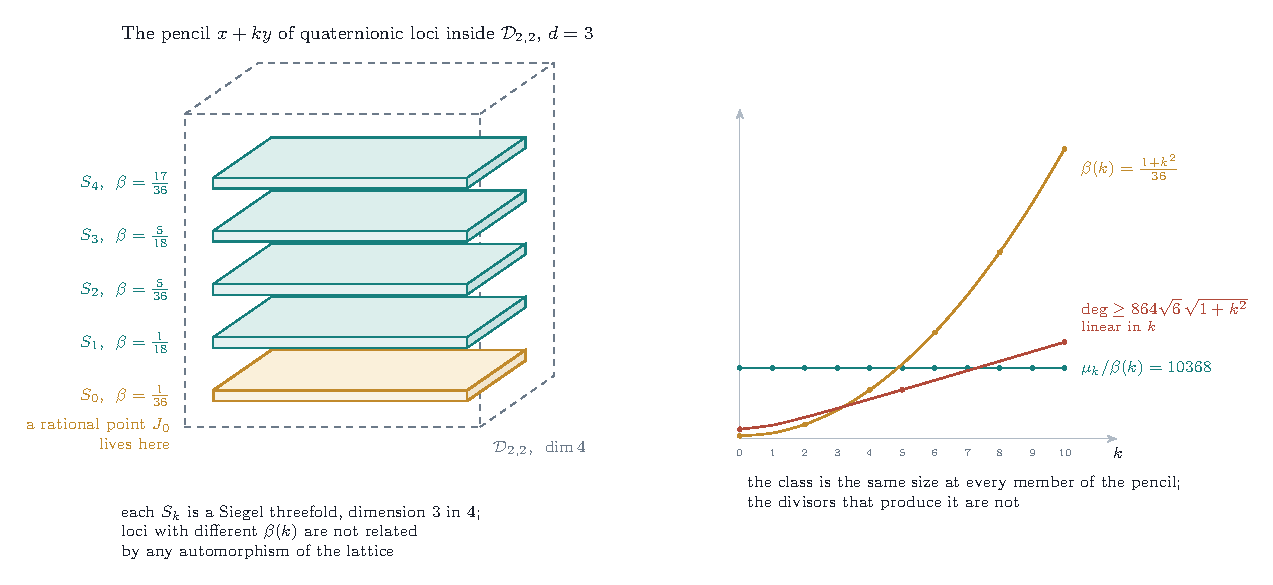
\includegraphics[width=\textwidth]{fig_pencil}
\caption{\Cref{prop:pencil} at $d=3$. Left: the members $S_{k}$ of the
pencil, each a Siegel threefold inside the four-dimensional family, with the
member $k=0$, where $\beta=\tfrac{1}{36}$ is a square and a rational point
$J_{0}$ can be written down, drawn apart. Right: along the pencil the ratio
$\mu_{k}/\beta(k)$ is the constant $10368=\int\eta^{4}/3$, so $\mu_{k}$
grows like $k^{2}$ and the least degree of a divisor not proportional to
$\eta$ grows linearly in $k$. The Weil class is a flat class of the one fixed
lattice and does not change; the divisors that produce it must.}
\label{fig:pencil}
\end{figure}

\begin{remark}[The case $n=2$]\label{rem:ntwo}
Let $n=2$, so $\dim\cS=n^{2}=4$. For every $n$ the quaternionic locus of
\Cref{setup:quat} has dimension $n(n+1)/2$, by a Morita argument. The
quaternion algebra $B=(-d,b)$ contains $K$ and acts on $V$, and
$B\otimes\RR\cong M_{2}(\RR)$ because $b>0$, so Morita equivalence writes
$V_{\RR}$ as $W\otimes_{\RR}\RR^{2}$ with $W$ symplectic of dimension $2n$.
The complex structures commuting with $B$ and compatible with $E$ are then
the complex structures on $W$ compatible with its symplectic form, that is the
points of the Siegel
space $\mathfrak{H}_{n}$, of dimension $n(n+1)/2$, and the codimension in
$\cD_{n,n}$ is $n^{2}-n(n+1)/2=n(n-1)/2$. At
$n=2$ the quaternionic locus is therefore the symmetric space of
$\Sp(4,\RR)$ inside $\cD_{2,2}$, of dimension $3$, so it is a divisor. Its
$G(\QQ)$-translates are infinitely many
pairwise distinct irreducible closed subvarieties of $\cS$ of dimension $3$,
since a finite union of proper closed analytic subsets cannot be dense. If
infinitely many of them carry cycles with one and the same data
$(\underline{P},\underline{q})$, then the closed set
$\Sigma_{\underline{P},\underline{q}}$ has an irreducible component containing
infinitely many distinct irreducible threefolds, so that component has
dimension at least $4$ and therefore equals $\cS$. No density is needed at
$n=2$, only infinitude. Combined with the theorem of Moonen and Zarhin
\cite{MZ99} that every Hodge class on an abelian fourfold lies in the
subalgebra generated by divisor classes and Weil classes, the conclusion would
be the Hodge conjecture for all abelian fourfolds of Weil type, hence for all
abelian fourfolds. That conclusion is a theorem of Markman
\cite[Corollary~1.6.1]{Mar25a}, proved by a different route, so at $n=2$ the
argument above would give a second proof; its interest lies in $n\ge3$.
\end{remark}

\section{Weil classes of every CM field}\label{sec:cmfields}

The Weil classes of an imaginary quadratic field are the case $m=1$ of a
construction that makes sense for every CM field $F$ of degree $2m$, and the
methods of this paper apply to the question whether those classes are
algebraic. Every theorem of \Cref{sec:construction} that turns the conjecture
for a Weil family into a propagation statement is a theorem about a connected
period domain, a flat class on it, a group whose rational points act with
dense orbits, and a base point where the class is a polynomial in divisor
classes, and none of these four ingredients depends on the field being
quadratic. This section carries the four over to every CM field; the only
one that needs a new argument is the base point, which
\Cref{thm:cmbasepoint} supplies. Nothing here is conditional on a question
about semiregularity, because the base point is a CM point: the Weil classes
there are written out as polynomials with rational coefficients in divisor
classes, each divisor class is algebraic by the Lefschetz theorem on $(1,1)$
classes, and products of algebraic classes are algebraic. Nothing is claimed
about the
whole Hodge ring at a CM point, which can contain classes that are not
polynomials in divisor classes.

\subsection{The families}

\begin{setupenv}[Weil type for a CM field]\label{setup:cmfield}
Let $F$ be a CM field of degree $2m$ with maximal totally real subfield
$F_{0}$, and write $\alpha\mapsto\bbar\alpha$ for the nontrivial automorphism
of $F/F_{0}$, which is complex conjugation under every embedding. The real
places of $F_{0}$ are $\tau_{1},\dots,\tau_{m}$, and each extends to a
conjugate pair $\sigma_{\tau},\bbar\sigma_{\tau}$ of embeddings of $F$ into
$\CC$. Let $V$ be an $F$-vector space of dimension $2n$, let
$H\colon V\times V\to F$ be a nondegenerate hermitian form, $F$-linear in the
first variable, and fix a totally imaginary $\xi\in F^{\times}$, that is
$\bbar\xi=-\xi$. Put
\[
  E(x,y)=\Tr_{F/\QQ}\bigl(\xi\,H(x,y)\bigr),
\]
a nondegenerate alternating $\QQ$-bilinear form with
$E(\alpha x,y)=E(x,\bbar\alpha y)$. For each $\tau$ let
$V_{\tau}=V\otimes_{F_{0},\tau}\RR$, a vector space of dimension $2n$ over
$F\otimes_{F_{0},\tau}\RR\cong\CC$, and let $(p_{\tau},q_{\tau})$ be the
signature of the hermitian form $H_{\tau}$ induced by $H$ on it. We say that
$(V,H)$ is of \emph{$(F,n)$-Weil type} if $p_{\tau}=q_{\tau}=n$ for every
$\tau$, and we call the class of $(-1)^{n}\det H$ in
$F_{0}^{\times}/\Nm_{F/F_{0}}(F^{\times})$ its discriminant $\delta$; it is
totally positive, and for $F=K$ it is the discriminant of \Cref{def:disc}. A
polarised abelian variety $(A,\iota,E)$ of dimension $2mn$ with
$\iota\colon F\to\End^{0}(A)$ and $H^{1}(A,\QQ)\cong V$ as $F$-modules with
polarisation $E$ is of $(F,n,\delta)$-Weil type when $(V,H)$ is. As in
\Cref{lem:Kspace}, we work throughout with $V=H^{1}$; a complex structure on
$V_{\RR}$ is the same datum as one on the tangent space. The Weil
classes of $A$ are
\[
  W_{F}(A)=\textstyle\bigwedge^{2n}_{F}V\;\subseteq\;\bigwedge^{2n}_{\QQ}V
  =H^{2n}(A,\QQ),
\]
the $\QQ$-subspace whose complexification is
$\bigoplus_{\sigma}\bigwedge^{2n}V_{\sigma}$, where $V_{\sigma}=V\otimes_{F,\sigma}\CC$
runs over the $2m$ eigenspaces of $F$ on $V_{\CC}$; it is a one-dimensional
$F$-vector space, of dimension $2m$ over $\QQ$. Write
\begin{quote}
$\mathbf{W}(F,n,\delta)$: every abelian variety of $(F,n,\delta)$-Weil type
has algebraic Weil classes.
\end{quote}
The period domain $\cD_{F}$ is the set of complex structures $J$ on
$V_{\RR}$ commuting with $F$ and polarised by $E$, and the group
$G_{F}=\Res_{F_{0}/\QQ}\SU(V,H)$ acts on it. We fix an arithmetic subgroup
$\Gamma\subset G_{F}(\QQ)$ and write $\cS_{F}=\Gamma\backslash\cD_{F}$ for the
quotient, $p\colon\cD_{F}\to\cS_{F}$ for the projection,
$\pi\colon\cA\to\cS_{F}$ for the universal family and
$\Sigma_{F}\subseteq\cD_{F}$ for the set of $s$ at which $W_{F}(A_{s})$ is
algebraic. For $m=1$ this is \Cref{setup:family} and \Cref{setup:shimura},
with $\omega_{s}$ a generator of the line.
\end{setupenv}

\begin{remark}[Every such abelian variety is a member]\label{rem:cmmember}
If $A$ is any abelian variety with a CM field $F\subseteq\End^{0}(A)$ such
that $\dim_{F}H^{1}(A,\QQ)=2n$ and $\dim V_{\sigma}^{1,0}=n$ for every
embedding $\sigma$, then $A$ is of $(F,n,\delta)$-Weil type for some
$\delta$: the Rosati involution of any polarisation restricts to a positive
involution of $F$, hence to conjugation, and the argument of
\Cref{lem:hermform} writes the polarisation as $\Tr_{F/\QQ}(\xi H)$ for a
unique hermitian $H$, whose signatures are then forced by the Hodge numbers
as in \Cref{prop:cmweil}(i). These are exactly the abelian varieties whose
Weil classes for $F$ are Hodge classes, in the sense of \cite{MZ99}, so
$\mathbf{W}(F,n,\delta)$ over all $(F,n,\delta)$ is the statement that all
Weil classes of all CM fields are algebraic.
\end{remark}

\begin{proposition}[The Weil classes of a CM field]\label{prop:cmweil}
Keep \Cref{setup:cmfield}, with $(V,H)$ of $(F,n)$-Weil type.
\begin{enumerate}[label=\textup{(\roman*)},leftmargin=2.6em,itemsep=2pt]
\item A polarised complex structure $J$ is the same as an $H_{\tau}$-orthogonal
  decomposition $V_{\tau}=V_{\tau}^{+}\oplus V_{\tau}^{-}$ for every $\tau$,
  with $H_{\tau}$ definite of the sign of $\mathrm{Im}\,\sigma_{\tau}(\xi)$ on
  $V_{\tau}^{+}$ and of the opposite sign on $V_{\tau}^{-}$; then
  $\dim V^{1,0}_{\sigma_{\tau}}=\dim V_{\tau}^{+}=n$ and
  $\dim V^{1,0}_{\bbar\sigma_{\tau}}=\dim V_{\tau}^{-}=n$, so every class in
  $W_{F}(A_{J})$ is of type $(n,n)$. The spaces $W_{F}(A_{J})$ form a flat
  subsystem $W_{F}$ of $R^{2n}\pi_{*}\QQ$ of rank $2m$ on which $G_{F}$ acts
  trivially, and $\cD_{F}\cong\prod_{\tau}\cD_{n,n}$ is connected of
  dimension $mn^{2}$.
\item If one nonzero element of $W_{F}(A)$ is algebraic, every element is.
\item If $\Hg(A_{s})=G_{F}$, the Hodge ring of $A_{s}$ is generated by
  $\NS(A_{s})_{\QQ}$ and by $W_{F}$, so the Hodge conjecture for $A_{s}$ in
  every degree is equivalent to the algebraicity of $W_{F}$. For $n\ge2$ the
  space $\NS(A_{s})_{\QQ}$ is the $m$-dimensional space of classes
  $\eta_{t}=[E(t\,\cdot,\cdot)]$, $t\in F_{0}$.
\item Two members of $(F,n,\delta)$-Weil type have isomorphic $(V,H)$, so
  every one of them is a fibre of $\pi$.
\end{enumerate}
\end{proposition}

\begin{proof}
(i) A complex structure commuting with $F$ preserves each $V_{\tau}$, since
$F_{0}\otimes\RR$ acts diagonally, and is $\CC$-linear on it for the
structure $F\otimes_{F_{0},\tau}\RR\cong\CC$, so it is $\pm\sqrt{-1}$ on two
complementary $\CC$-subspaces $V_{\tau}^{\pm}$. Write
$\sigma_{\tau}(\xi)=\sqrt{-1}\,r_{\tau}$ with $r_{\tau}\in\RR^{\times}$. For
$x\in V^{\epsilon}_{\tau}$ and $y\in V^{\epsilon'}_{\tau}$ one has
$H_{\tau}(Jx,Jy)=\epsilon\epsilon'H_{\tau}(x,y)$, so
$E(Jx,Jy)=E(x,y)$ forces $E(x,y)=0$ for $\epsilon\ne\epsilon'$, and replacing
$x$ by $\sqrt{-1}\,x$ then forces $H_{\tau}(x,y)=0$: the decomposition is
orthogonal. For $x\in V^{\epsilon}_{\tau}$,
$E(x,Jx)=2\,\mathrm{Re}\bigl(\sqrt{-1}\,r_{\tau}\,
\overline{\epsilon\sqrt{-1}}\,H_{\tau}(x,x)\bigr)=2\epsilon r_{\tau}H_{\tau}(x,x)$,
so positivity is the sign condition stated. Conversely such a decomposition
defines a polarised $J$. Under $V_{\tau}\otimes_{\RR}\CC=V_{\sigma_{\tau}}
\oplus V_{\bbar\sigma_{\tau}}$ the space $V^{1,0}$, the $\sqrt{-1}$-eigenspace
of $J$ on $V_{\CC}$, meets $V_{\sigma_{\tau}}$ in the image of $V_{\tau}^{+}$
and $V_{\bbar\sigma_{\tau}}$ in the conjugate of the image of $V_{\tau}^{-}$,
which gives the two equalities of dimensions. Since $H_{\tau}$ has signature
$(n,n)$ and is definite, of opposite signs, on the complementary orthogonal
subspaces $V_{\tau}^{\pm}$, both have dimension $n$. So each $V_{\sigma}$ is
the sum of its intersections with $V^{1,0}$ and $V^{0,1}$, both of dimension
$n$, and a generator $\alpha_{\sigma}$ of $\bigwedge^{2n}V_{\sigma}$ is of
type $(n,n)$. The subspace $\bigwedge^{2n}_{F}V$ of $H^{2n}(A_{s},\QQ)$ is
defined by the action of $F$ on $V$ alone and does not depend on $s$, so it
is flat; $\SU(V,H)$ acts on $\bigwedge^{2n}_{F}V$ by the $F$-determinant,
which is $1$. Finally, the choice of $V_{\tau}^{+}$ is a point of the bounded
symmetric domain of $\SU(V_{\tau},H_{\tau})\cong\SU(n,n)$, of dimension
$n^{2}$, and $\cD_{F}$ is the product over $\tau$.

(ii) For $\alpha\in\cO_{F}$ the endomorphism $\iota(\alpha)$ acts on
$\bigwedge^{2n}_{F}V$ by $\alpha^{2n}$, through an algebraic correspondence,
so the algebraic classes in $W_{F}$ form a $\QQ$-subspace stable under
multiplication by every $\alpha^{2n}$. By the polarisation identity, in
characteristic zero every product $x_{1}\cdots x_{2n}$ of elements of a field
is a rational combination of $2n$-th powers of sums of the $x_{i}$; taking
$x_{2}=\dots=x_{2n}=1$ shows that the $2n$-th powers span $F$ over $\QQ$, and
since every element of $F$ is a rational multiple of an element of $\cO_{F}$,
so do the $\alpha^{2n}$ with $\alpha\in\cO_{F}$. Hence the $\QQ$-span of
$\{\alpha^{2n}w\}$ is $Fw=W_{F}$ for every $w\ne0$.

(iii) Hodge classes are the invariants of the Hodge group, which here is
$G_{F}$. Over $\CC$ it is $\prod_{\tau}\SL(U_{\tau})$ with
$U_{\tau}=V_{\sigma_{\tau}}$, and
$H$ identifies $V_{\bbar\sigma_{\tau}}$ with $U_{\tau}^{\vee}$, so
$\bigwedge^{*}V_{\CC}=\bigotimes_{\tau}\bigwedge^{*}(U_{\tau}\oplus U_{\tau}^{\vee})$
with the $\tau$-th factor of the group acting on the $\tau$-th tensor factor
alone. The invariants of a product group in a tensor product of
representations are the tensor product of the invariants, and the invariants
of $\SL(U)$ in $\bigwedge^{*}(U\oplus U^{\vee})$ are generated by the pairing
$\psi\in U\otimes U^{\vee}$ and the two determinants, by the computation of
\Cref{thm:hdgcount}. The classes $\eta_{t}$ are Hodge classes: $J$ commutes
with $t$ and preserves $E$, hence preserves the $F_{0}$-twisted form
$E_{t}=E(t\,\cdot,\cdot)=\Tr(\xi tH)$, which for totally positive $t$ is again
a polarisation of $A_{s}$. The complexified span of the $\eta_{t}$ is
$\bigoplus_{\tau}\CC\psi_{\tau}$, and the complexification of $W_{F}$
contains all the determinants. So the $\QQ$-algebra generated by $\NS_{\QQ}$
and $W_{F}$ has complexification equal to the ring of invariants, hence
equals $\Hdg^{*}(A_{s})$. Since divisor classes are algebraic, the conjecture
reduces to $W_{F}$, and by (ii) to one class. For the last sentence, the
invariants in $\bigwedge^{2}V_{\CC}$ are $\bigoplus_{\tau}\CC\psi_{\tau}$ when
$n\ge2$: a summand $\bigwedge^{2}U_{\tau}$ or $\bigwedge^{2}U_{\tau}^{\vee}$
has an $\SL(U_{\tau})$-invariant only if $\dim U_{\tau}=2n$ equals $2$, and a
summand mixing two different $\tau$ has none. So $\NS(A_{s})_{\QQ}$ has
dimension $m$, and it contains the classes $\eta_{t}$, which form an
$m$-dimensional space because $t\mapsto\eta_{t}$ is injective on $F_{0}$, $E$
being nondegenerate.

(iv) Two hermitian forms over $F/F_{0}$ of the same rank, the same
discriminant and the same signature at every real place of $F_{0}$ are
isomorphic \cite[Ch.~10, \S6]{Sch85}. So the datum $(F,n,\delta)$ determines
$(V,H)$ up to isomorphism, and the Hodge structure of any member is, by (i), a
polarised complex structure on that $V_{\RR}$, that is a point of $\cD_{F}$.
\end{proof}

\begin{lemma}[The Hodge group of a very general member]\label{lem:cmgeneric}
Keep \Cref{setup:cmfield}. For every $s\in\cD_{F}$ one has
$\Hg(A_{s})\subseteq G_{F}$, and there is a countable union $Z$ of proper
closed analytic subsets of $\cD_{F}$ such that $\Hg(A_{s})=G_{F}$ for every
$s\notin Z$.
\end{lemma}

\begin{proof}
The Hodge group of $A_{s}$ commutes with $\End^{0}(A_{s})\supseteq F$ and
preserves $E$, so it lies in $\Res_{F_{0}/\QQ}\mathrm{U}(V,H)$: an $F$-linear
map preserving $E=\Tr_{F/\QQ}(\xi H)$ preserves $H$, because $H$ is recovered
from $E$ and the action of $F$ as in \Cref{lem:hermform}. It fixes every Hodge
class, in particular the Weil classes, which are Hodge classes by
\Cref{prop:cmweil}(i); an element $g$ of $\Res_{F_{0}/\QQ}\mathrm{U}(V,H)$ acts
on $\bigwedge^{2n}_{F}V$ by $\det_{F}(g)$, so $\det_{F}(g)=1$ and
$g\in G_{F}$.

For the second statement let $T$ be the set of rational tensors
$t\in\bigoplus_{a,b}V^{\otimes a}\otimes(V^{\vee})^{\otimes b}$ that are not
fixed by $G_{F}$, a countable set, and for $t\in T$ let $Z_{t}$ be the set of
$s$ at which $t$ is a Hodge class, of type $(p,p)$ with $2p=a-b$, for the
Hodge structure induced by $A_{s}$. The condition is that $t$ lies in the
$p$-th step of the Hodge filtration, which varies holomorphically with $s$, so
$Z_{t}$ is a closed analytic subset of $\cD_{F}$. It is proper. Otherwise $t$
is fixed by $h_{s}(\mathrm{U}(1))$ for every $s\in\cD_{F}$, where $h_{s}$ is
the Hodge representation, which acts on the $(p,q)$ part through
$z^{q-p}$, and hence by the
subgroup $N$ of $G_{F}(\RR)$ that these tori generate. Since $\cD_{F}$ is one
orbit of $G_{F}(\RR)^{+}$ and $h_{gs}=gh_{s}g^{-1}$, the group $N$ is a
connected normal subgroup of $G_{F}(\RR)^{+}=\prod_{\tau}\SU(V_{\tau},H_{\tau})$,
so its Lie algebra is an ideal of
$\bigoplus_{\tau}\mathfrak{su}(V_{\tau},H_{\tau})$, a sum of some of these
simple summands. It contains every summand, because $h_{s}(\sqrt{-1})$ acts on
$V_{\tau}$ as the complex structure $J$, which is $\sqrt{-1}$ on
$V^{+}_{\tau}$ and $-\sqrt{-1}$ on $V^{-}_{\tau}$ by \Cref{prop:cmweil}(i),
and is therefore not central in the factor $\SU(V_{\tau},H_{\tau})$. So
$N=G_{F}(\RR)^{+}$, which is Zariski dense in the connected group $G_{F}$,
and $t$ would be fixed by $G_{F}$, contrary to $t\in T$.

Put $Z=\bigcup_{t\in T}Z_{t}$. The Hodge group of $A_{s}$ is the subgroup of
$\GL(V)$ fixing every rational Hodge class in the spaces
$V^{\otimes a}\otimes(V^{\vee})^{\otimes b}$ \cite[\S3]{Del82}.
For $s\notin Z$ each such class is fixed by $G_{F}$, so
$G_{F}\subseteq\Hg(A_{s})$, and equality follows from the first statement.
\end{proof}

\subsection{A base point in every family}

\begin{theorem}[A base point in every family, for every CM field]
\label{thm:cmbasepoint}
Let $(V,H)$ be of $(F,n)$-Weil type with discriminant $\delta$. Then $\cD_{F}$
contains a point $s_{0}$ with the following properties.
\begin{enumerate}[label=\textup{(\roman*)},leftmargin=2.6em,itemsep=2pt]
\item $A_{s_{0}}$ is isogenous to $B_{\Phi}^{\,n}\times B_{\bbar\Phi}^{\,n}$,
  where $B_{\Phi}$ is an abelian $m$-fold with complex multiplication by $F$
  of type $\Phi=\{\sigma:\mathrm{Im}\,\sigma(\xi)>0\}$ and $B_{\bbar\Phi}$ its
  conjugate; there is an $H$-orthogonal basis $e_{1},\dots,e_{2n}$ of $V$
  with $H(e_{i},e_{i})$ totally positive for $i\le n$ and totally negative
  for $i>n$, and $Fe_{i}=H^{1}(B_{\Phi},\QQ)$ for $i\le n$,
  $Fe_{i}=H^{1}(B_{\bbar\Phi},\QQ)$ for $i>n$.
\item For $i\le n$ put $i'=i+n$ and let $D_{ii'}\subseteq H^{2}(A_{s_{0}},\QQ)$
  be the $F$-balanced part of $Fe_{i}\wedge Fe_{i'}$, spanned by the classes
  \[
    \delta_{i}(f)=\sum_{k}\,(\omega_{k}f\,e_{i})\wedge(\omega_{k}^{*}\,e_{i'}),
    \qquad f\in F,
  \]
  for dual $\QQ$-bases $(\omega_{k})$, $(\omega_{k}^{*})$ of $F$ with respect
  to the trace form. Every $\delta_{i}(f)$ is a Hodge class of type $(1,1)$,
  hence a divisor class, and $D_{ii'}$ is a one-dimensional $F$-vector space
  with $\alpha\cdot\delta_{i}(f)=\delta_{i}(\alpha f)$.
\item The Weil classes are the products
  \[
    w(f)=\sum_{k_{1},\dots,k_{n-1}}
      \delta_{1}(\omega_{k_{1}}f)\cdot\delta_{2}(\omega_{k_{1}}^{*}\omega_{k_{2}})
      \cdots\delta_{n-1}(\omega_{k_{n-2}}^{*}\omega_{k_{n-1}})\cdot
      \delta_{n}(\omega_{k_{n-1}}^{*}),\qquad f\in F,
  \]
  which lie in $W_{F}(A_{s_{0}})$, span it as $f$ runs over $F$, and are
  polynomials with rational coefficients in divisor classes. In particular
  $W_{F}(A_{s_{0}})$ is algebraic, and $\Sigma_{F}\ne\emptyset$ for every $F$,
  every $n\ge1$ and every $\delta$.
\end{enumerate}
\end{theorem}

\begin{proof}
(i) Since $H_{\tau}$ has signature $(n,n)$ at every $\tau$, the determinant
$\det H$ has sign $(-1)^{n}$ at every real place, so $b=(-1)^{n}\det H$, a
representative of $\delta$, is totally positive, and the diagonal form $H'=\mathrm{diag}(b,1,\dots,1,-1,\dots,-1)$
with $n$ positive and $n$ negative entries has the same dimension, the same
discriminant and the same signatures as $H$. Hermitian forms over $F/F_{0}$
are classified by these invariants \cite[Ch.~10, \S6]{Sch85}, so
$(V,H)\cong(F^{2n},H')$ and the standard basis is the required orthogonal
basis $e_{i}$, with $a_{i}=H(e_{i},e_{i})$. Write $\sigma_{\tau}(\xi)=\sqrt{-1}\,r_{\tau}$
and define $J$ on $V_{\tau}=\bigoplus_{i}\CC e_{i}$ to be
$\epsilon_{i,\tau}\sqrt{-1}$ on $\CC e_{i}$, with
$\epsilon_{i,\tau}=\mathrm{sign}(r_{\tau})\,\mathrm{sign}(\tau(a_{i}))$. The
decomposition $V_{\tau}^{+}=\bigoplus_{\epsilon_{i,\tau}=+}\CC e_{i}$,
$V_{\tau}^{-}=\bigoplus_{\epsilon_{i,\tau}=-}\CC e_{i}$ is $H_{\tau}$-orthogonal,
with $H_{\tau}$ of sign $\mathrm{sign}(r_{\tau})$ on $V_{\tau}^{+}$ and of the
opposite sign on $V_{\tau}^{-}$, so \Cref{prop:cmweil}(i) makes $J$ a point
$s_{0}$ of $\cD_{F}$. On $Fe_{i}\otimes\RR=\prod_{\tau}\CC e_{i}$ the
structure $J$ is multiplication by the element
$(\epsilon_{i,\tau}\sqrt{-1})_{\tau}$ of $F\otimes_{\QQ}\RR$, so each $Fe_{i}$
is a rational sub-Hodge structure of weight one with $F$-action, polarised by
the restriction of $E$; that is, it is the $H^{1}$ of an abelian $m$-fold with
complex multiplication by $F$, of CM type
$\Phi_{i}=\{\sigma:(Fe_{i})_{\sigma}\subseteq V^{1,0}\}$, which by the
computation in \Cref{prop:cmweil}(i) is
$\{\sigma_{\tau}^{\epsilon_{i,\tau}}\}$, where $\sigma^{+}=\sigma$ and
$\sigma^{-}=\bbar\sigma$. For $i\le n$ the $a_{i}$ are totally positive, so
$\epsilon_{i,\tau}=\mathrm{sign}(r_{\tau})$ and
$\Phi_{i}=\{\sigma:\mathrm{Im}\,\sigma(\xi)>0\}=\Phi$; for $i>n$ the signs are
reversed and $\Phi_{i}=\bbar\Phi$. So $V=\bigoplus_{i}Fe_{i}$ splits
$A_{s_{0}}$ up to isogeny as stated.

(ii) Write $L_{i,\sigma}=(Fe_{i})_{\sigma}$, a line, so that
$V_{\CC}=\bigoplus_{i,\sigma}L_{i,\sigma}$ and $L_{i,\sigma}$ has type $(1,0)$
exactly when $\sigma\in\Phi_{i}$. For dual bases,
$\sum_{k}\sigma(\omega_{k})\sigma'(\omega_{k}^{*})=1$ if $\sigma=\sigma'$ and
$0$ otherwise, because the matrices $(\sigma(\omega_{k}))$ and
$(\sigma(\omega_{k}^{*}))$ are inverse transposes by the definition of the
trace form. Let $\ell_{i,\sigma}$ be the component of $e_{i}$ in
$L_{i,\sigma}$, a generator of that line, so that
$\omega e_{i}=\sum_{\sigma}\sigma(\omega)\,\ell_{i,\sigma}$ for $\omega\in F$.
Hence in $Fe_{i}\otimes Fe_{i'}\otimes\CC
=\bigoplus_{\sigma,\sigma'}L_{i,\sigma}\otimes L_{i',\sigma'}$ the class
$\delta_{i}(f)$ has component $\sigma(f)\,\ell_{i,\sigma}\wedge\ell_{i',\sigma}$
on the diagonal $\sigma=\sigma'$ and zero off it. In particular it is
$F$-balanced: $\alpha\in F$ acting through the first factor and through the
second agree on it, both multiplying the component at $\sigma$ by
$\sigma(\alpha)$, and this is the identity
$\alpha\cdot\delta_{i}(f)=\delta_{i}(\alpha f)$. Since $\Phi_{i'}=\bbar\Phi_{i}$,
exactly one of $L_{i,\sigma}$, $L_{i',\sigma}$ has type $(1,0)$, so every
component, hence $\delta_{i}(f)$, has type $(1,1)$; and $\delta_{i}(f)$ is
rational, being a sum of wedges of rational vectors. By the Lefschetz theorem
on $(1,1)$ classes it is a divisor class. As $f$ varies the components
$\sigma(f)$ vary independently, so $D_{ii'}\otimes\CC=\bigoplus_{\sigma}
L_{i,\sigma}\otimes L_{i',\sigma}$ and $D_{ii'}\cong F$.

(iii) The complexification of $W_{F}$ is spanned by
$\alpha_{\sigma}=\pm\prod_{i\le n}\ell_{i,\sigma}\wedge\ell_{i',\sigma}$, a
generator of $\bigwedge^{2n}V_{\sigma}=\bigwedge^{2n}\bigl(\bigoplus_{i}L_{i,\sigma}\bigr)$.
In the product $w(f)$, the component indexed by $(\sigma_{1},\dots,\sigma_{n})$,
with $\sigma_{i}$ the embedding chosen in the $i$-th factor, carries the
coefficient
$\sigma_{1}(f)\prod_{j=1}^{n-1}\sum_{k_{j}}\sigma_{j}(\omega_{k_{j}})\sigma_{j+1}(\omega_{k_{j}}^{*})$,
which vanishes unless $\sigma_{1}=\dots=\sigma_{n}$ and then equals
$\sigma_{1}(f)$. So $w(f)=\sum_{\sigma}\sigma(f)\,\alpha_{\sigma}$ up to the
sign of the reordering, an element of $W_{F}\otimes\CC$ which is rational
because it is a rational polynomial in rational classes; as $f$ runs over
$F$ the vectors $(\sigma(f))_{\sigma}$ span $\CC^{2m}$, so the $w(f)$ span
$W_{F}$. Each $w(f)$ is a rational combination of $n$-fold products of the
divisor classes $\delta_{i}(\cdot)$, and a product of divisor classes is
algebraic.
\end{proof}

\begin{remark}[The base point for a quadratic field]\label{rem:cmquadratic}
For $m=1$ the point $s_{0}$ is a member isogenous to $E^{2n}$ for an elliptic
curve $E$ with complex multiplication by $K$, at which the whole Hodge ring
is generated by divisor classes, since the Hodge group is a one-dimensional
torus. It is a second base point in every family of \Cref{sec:construction},
beside the quaternionic one of \Cref{thm:everyfamily}, and it lies in the
product locus of \Cref{thm:everyn}. The formula of
\Cref{thm:cmbasepoint}(iii) then gives the class at that point explicitly.
\end{remark}

\subsection{The reduction and the propagation}\label{ssec:cmpropagation}

\begin{theorem}[The reduction and the propagation, for every CM field]
\label{thm:cmpropagation}
Fix $(F,n,\delta)$ with $n\ge2$, keep \Cref{setup:cmfield}, and let
$\omega_{s}$ denote a generator of $W_{F}(A_{s})$ chosen flatly.
\begin{enumerate}[label=\textup{(\roman*)},leftmargin=2.6em,itemsep=2pt]
\item $\mathbf{W}(F,n,\delta)$ holds if and only if $\omega_{s}$ is algebraic
  for every $s\in\cD_{F}$, and then the Hodge conjecture holds in every
  degree for every member of the family with $\Hg(A_{s})=G_{F}$.
\item $\Sigma_{F}$ is stable under $G_{F}(\QQ)$, every $G_{F}(\QQ)$-orbit in
  $\cD_{F}$ is dense, and $\Sigma_{F}$ is dense.
\item $\Sigma_{F}=p^{-1}\bigl(\bigcup_{\underline{P},\underline{q}}
  \Sigma_{\underline{P},\underline{q}}\bigr)$ with each
  $\Sigma_{\underline{P},\underline{q}}$ Zariski closed in $\cS_{F}$, the
  union countable; either $\Sigma_{F}=\cD_{F}$, or $\Sigma_{F}$ is meagre and
  the conjecture fails on a dense $G_{\delta}$.
\item If at every point $s$ of the orbit $G_{F}(\QQ)\cdot s_{0}$ the class
  $\omega_{s}$ is represented by a cycle whose Hilbert data comes from one
  finite set, then $\Sigma_{F}=\cD_{F}$.
\item If some perfect complex $E$ on $A_{s_{0}}$ with
  $\ch(E)=N\omega_{s_{0}}+P$, where $N\ne0$ and $P$ is a polynomial with
  rational coefficients in the classes $\eta_{t}$ of
  \Cref{prop:cmweil}(iii), has injective semiregularity map, then
  $\Sigma_{F}=\cD_{F}$. Complexes with $\ch(E)=N\omega_{s_{0}}$ exist.
\end{enumerate}
\end{theorem}

\begin{proof}
(i) By \Cref{prop:cmweil}(i) and (iv), every member has its Hodge structure
at some point of $\cD_{F}$, so $\mathbf{W}(F,n,\delta)$ is the algebraicity of
$W_{F}$ at every point. By \Cref{prop:cmweil}(ii) this is the algebraicity of
one generator at every point, and by \Cref{prop:cmweil}(iii) it gives the
conjecture at the members with full Hodge group.

(ii) The stability is the argument of \Cref{lem:Ginvariance}: $g\in G_{F}(\QQ)$
carries $J$ to $gJg^{-1}$ and induces, after clearing denominators, an isogeny
$A_{J}\to A_{gJ}$ whose graph transports algebraic classes to algebraic
classes, and $g$ fixes $W_{F}$ pointwise by \Cref{prop:cmweil}(i).

For the density we show that the closure $L$ of $G_{F}(\QQ)$ in
$G_{F}(\RR)=\prod_{\tau}\SU(V_{\tau},H_{\tau})$ contains the identity
component, which acts transitively on $\cD_{F}$. First, the form $H$ is
isotropic over $F_{0}$. It is indefinite at every real place, its signature
being $(n,n)$. At every finite place $v$ its trace form is a quadratic form
in $4n\ge8$ variables over the local field $F_{0,v}$, hence isotropic, and a
hermitian form is isotropic as soon as its trace form is
\cite[Ch.~10, \S1]{Sch85}. Since hermitian forms over the quadratic
extension $F/F_{0}$ satisfy the Hasse principle \cite[Ch.~10, \S6]{Sch85},
$H$ is isotropic. Let $X=\{v\in V:H(v,v)=0\}$ be the cone of isotropic
vectors, a quadric cone in the $4n$-dimensional $F_{0}$-space $V$ with a
nonzero $F_{0}$-point. Projection from that point shows that the projective
quadric of its lines is $F_{0}$-rational, that is, $F_{0}$-birational to a
projective space, so it satisfies weak approximation at the archimedean
places, $F_{0}$ being dense in $F_{0}\otimes\RR=\prod_{\tau}\RR$. Hence the
$F_{0}$-points of $X$ are dense in its points over $F_{0}\otimes\RR$, which
are the products $\prod_{\tau}X_{\tau}$ of the isotropic cones of the
$H_{\tau}$.

For an isotropic vector $v\in V$ let $U_{v}\subseteq\SU(V,H)$ be the
unipotent radical of the stabiliser of the line $Fv$, a unipotent
$F_{0}$-group. The exponential identifies $U_{v}(F_{0})$ with an
$F_{0}$-vector space and $U_{v}(F_{0}\otimes\RR)=\prod_{\tau}U_{v,\tau}(\RR)$
with the corresponding real space, so $U_{v}(\QQ)=U_{v}(F_{0})$ is dense in
$\prod_{\tau}U_{v,\tau}(\RR)$. Hence $L$ contains
$\prod_{\tau}U_{v,\tau}(\RR)$ for every rational isotropic $v$, in particular
the factor $U_{v,\tau}(\RR)$ for each $\tau$ separately, and its Lie algebra
$\mathfrak{l}$ contains $\mathfrak{u}_{v,\tau}$ for every $\tau$ and every
rational isotropic $v$. The map $v\mapsto\mathfrak{u}_{v,\tau}$ is continuous
on $X_{\tau}\setminus0$ and rational $v$ are dense in
$\prod_{\tau}X_{\tau}$, so the closed subspace
$\mathfrak{l}\cap\mathfrak{su}(V_{\tau},H_{\tau})$ contains
$\mathfrak{u}_{v,\tau}$ for every isotropic $v\in V_{\tau}$. The span of these
is stable under the adjoint action of $\SU(V_{\tau},H_{\tau})$, which permutes
the isotropic lines, so it is a nonzero ideal of the simple Lie algebra
$\mathfrak{su}(n,n)$, hence everything. Thus
$\mathfrak{l}\supseteq\bigoplus_{\tau}\mathfrak{su}(V_{\tau},H_{\tau})$ and
$L\supseteq G_{F}(\RR)^{+}$, so every $G_{F}(\QQ)$-orbit in $\cD_{F}$ is
dense. Since $\Sigma_{F}$ is nonempty by \Cref{thm:cmbasepoint} and
$G_{F}(\QQ)$-stable, it contains a dense orbit.

(iii) The proofs of \Cref{thm:closedlocus} and \Cref{cor:allornothing} use
only three facts: that $\cS_{F}$ is a quasi-projective variety, by the
theorem of Baily and Borel \cite{BB66}; that the relative Hilbert schemes of
$\cA/\cS_{F}$ are projective over it \cite{Gro61}; and that $W_{F}$ is a flat
subsystem consisting of Hodge classes, which is \Cref{prop:cmweil}(i). They
apply verbatim.

(iv) The argument is the proof of \Cref{thm:degreebound}, which asks for a
cycle chosen at each point (\Cref{rem:chosencycle}). The orbit is dense by
(ii), and a finite union of the closed sets of (iii) covering it forces one of
them to be dense and closed, hence everything; then (i) applies. As in the
quadratic case, the hypothesis is equivalent to the conclusion
(\Cref{thm:p1equivalent}), and the transported cycle does not satisfy it
(\Cref{thm:p1forces}).

(v) The existence of complexes with $\ch(E)=N\omega_{s_{0}}$ is the proof of
\cite[Proposition~2.1]{paperII}, applied to the algebraic cycle of \Cref{thm:cmbasepoint}
with the isomorphism $K_{0}(A)_{\QQ}\cong\CH^{*}(A)_{\QQ}$ \cite{Ful98}. The
deformation argument is the proof of \cite[Theorem~2.3]{paperII} for a
polarised Chern character, as in \cite[Remark~3.6]{paperII}. Its only inputs are
the theorem of Buchweitz and Flenner, (iii), and the flatness of $\ch(E)$ as
a section of Hodge classes over $\cD_{F}$; the last holds because $W_{F}$ is
flat by \Cref{prop:cmweil}(i) and the classes $\eta_{t}$ remain of Hodge type
on the whole family, as in the proof of \Cref{prop:cmweil}(iii). At a member
$A_{s}$ reached by the deformation the component of degree $2n$ of the
character is $N\omega_{s}+P_{2n}$, with $P_{2n}$ a polynomial in divisor
classes, so $\omega_{s}$ is algebraic.
\end{proof}

\begin{corollary}[The Hodge conjecture for the very general member]
\label{cor:verygeneral}
Fix $(F,n,\delta)$ with $n\ge2$. The following are equivalent.
\begin{enumerate}[label=\textup{(\alph*)},leftmargin=2.6em,itemsep=2pt]
\item $\Sigma_{F}$ is closed in $\cD_{F}$.
\item $\Sigma_{F}$ has an interior point.
\item $\Sigma_{F}=\cD_{F}$, that is, the Weil classes are algebraic on every
  member of the family.
\item The Hodge conjecture holds for the very general member of the family:
  there is a countable union of proper closed analytic subsets of $\cD_{F}$
  outside which the Hodge conjecture holds for $A_{s}$ in every degree.
\end{enumerate}
\end{corollary}

\begin{proof}
If (a) holds, $\Sigma_{F}$ is closed and dense by
\Cref{thm:cmpropagation}(ii), so (c) holds; and (c) implies (a) and (b). If
(b) holds, $\Sigma_{F}$ is not meagre, since a nonempty open subset of the
manifold $\cD_{F}$ is not meagre by Baire's theorem, and
\Cref{thm:cmpropagation}(iii) gives (c). If (c) holds, the Hodge conjecture
holds in every degree for every member with $\Hg(A_{s})=G_{F}$ by
\Cref{thm:cmpropagation}(i), and these are the members outside the set $Z$ of
\Cref{lem:cmgeneric}, so (d) holds. Finally, if (d) holds with an exceptional
set $Z'$, then at every $s\notin Z'$ the Weil classes, which are Hodge classes
at every point by \Cref{prop:cmweil}(i), are algebraic. So $\Sigma_{F}$
contains the complement of $Z'$, which is not meagre by Baire's theorem,
since each proper closed analytic subset of the connected manifold $\cD_{F}$
is nowhere dense; by \Cref{thm:cmpropagation}(iii), $\Sigma_{F}=\cD_{F}$.
\end{proof}

\begin{proof}[Proof of \Cref{thm:main}]
Part (i) is \Cref{thm:cmbasepoint}, parts (ii) and (iii) are
\Cref{thm:cmpropagation}(ii) and (iii), and part (iv) is
\Cref{cor:verygeneral}.
\end{proof}

\begin{remark}[Scope of the reduction]\label{rem:cmwhatisnew}
The propagation statements (iv) and (v) are exactly the two forms (P1) and
(P2) of \cite[Remark~3.7]{paperII} with $F$ in place of $K$, (v) being (P2) in the
polarised form of \cite[Remark~3.6]{paperII}. This section proves that they are the
whole of the problem for every CM field, and that their hypothesis is never
vacuous: the base point exists, its cycle is written down, and the orbit
through it is dense. The theorem of \cite[Theorem~2.5]{paperII} on what (v) forces
transfers as well, with the annihilator of a class in $W_{F}$ computed over
the $2m$ eigenspaces in place of two, and we do not repeat it. Nothing above
depends on Question 11.4 of \cite{Mar25b} or on any secant construction. The
route through Weil restriction and CM points is independent of the route
through secant sheaves and reaches every field at once; Markman has extended
the route through secant sheaves to these fields \cite{Mar25c} (see (C3) in
\cite[Section~2.5]{paperIII}, and \cite[Section~5.2]{paperII} for the smallest case).
\end{remark}

\begin{proposition}[Composite fields]\label{prop:composite}
Let $F=KF_{0}$ with $K$ imaginary quadratic, and let $A$ be of
$(F,n,\delta)$-Weil type. Then $A$ is of $(K,-1,mn)$-Weil type for the
restricted action, its Weil classes $W_{K}(A)\subseteq H^{2mn}(A,\QQ)$ lie in
the $\QQ$-span of the $m$-fold products of elements of $W_{F}(A)$, and
$W_{K}(A)$ is algebraic whenever $W_{F}(A)$ is. In particular
$\mathbf{W}(F,n,\delta)$ implies the algebraicity of the $K$-Weil classes on
every member of the $F$-family, a closed subvariety of dimension $mn^{2}$ of
the $K$-family of dimension $m^{2}n^{2}$; the converse implication is not
available, and \Cref{thm:cmbasepoint} is not a consequence of
\Cref{thm:everyfamily}.
\end{proposition}

\begin{proof}
The eigenspace $V_{\tau_{K}}$ of $K$ on $V_{\CC}$ for the embedding
$\tau_{K}$ is $\bigoplus_{\sigma|\tau_{K}}V_{\sigma}$, of dimension $2mn$
with $\dim V_{\tau_{K}}^{1,0}=mn$ by \Cref{prop:cmweil}(i), so $A$ is of
$K$-Weil type with balanced signature, and
$\bigwedge^{2mn}V_{\tau_{K}}=\bigotimes_{\sigma|\tau_{K}}\bigwedge^{2n}V_{\sigma}$
is spanned by $\prod_{\sigma|\tau_{K}}\alpha_{\sigma}$. So
$W_{K}\otimes\CC$ is contained in the complexification of the $\QQ$-span $P$ of
the $m$-fold products of elements of $W_{F}$, and a rational subspace whose
complexification lies in that of $P$ lies in $P$. Since products of
algebraic classes are algebraic, $W_{K}(A)$ is algebraic whenever $W_{F}(A)$
is. The last sentence of the statement is a dimension count:
for $m\ge2$ the $F$-family is a proper subvariety of the $K$-family, and the
$K$-Weil classes on it are products that carry no information about their
factors.
\end{proof}

\subsection{The special locus and an escaping sequence}
\label{ssec:speciallocus}

The properties of $\Sigma_{F}$ proved so far are shared by a set that is
meagre, the locus of members whose Hodge group is smaller than
$G_{F}$, and every construction of algebraic Weil classes available for
$n\ge4$ produces points of that locus only. In the other direction the
bounded criterion (iv) of \Cref{thm:cmpropagation} needs far less than an
orbit: by the theorem of Pila, Shankar and Tsimerman on the Andr\'e--Oort
conjecture, a bound on one sequence of CM points that leaves every proper
special subvariety is enough (\Cref{fig:speciallocus}).

\begin{definition}[Special subvarieties and the special locus]
\label{def:speciallocus}
Keep \Cref{setup:cmfield}, with $\Gamma$ a congruence subgroup. A
\emph{special subvariety} of $\cS_{F}$ is an irreducible component of the
image in $\cS_{F}$ of a connected component of the locus of Hodge classes
$\Hdg^{p}(\mathbb{V})$, where $\mathbb{V}$ runs over the variations
$(R^{1}\pi_{*}\ZZ)^{\otimes a}\otimes(R^{1}\pi_{*}\ZZ)^{\vee\,\otimes b}$
of even weight, or $\cS_{F}$ itself; these are the special subvarieties of
$\cS_{F}$ for $R^{1}\pi_{*}\ZZ$ in the sense of \cite{KOU}.%
\footnote{By a theorem of Chevalley every algebraic subgroup of $\GL(V)$ is
the stabiliser of finitely many tensors \cite[\S3]{Del82}, so the locus where
the Hodge group lies in a given subgroup is a locus of Hodge tensors, and
these subvarieties are the special subvarieties of $\cS_{F}$ as a connected
Shimura variety, the images of the domains of the reductive subgroups of
$G_{F}$ that contain the Hodge group of one of their points.}
A \emph{CM point} is a point $p(s)$ at which $A_{s}$ is of CM type, that is,
at which $\Hg(A_{s})$ is a torus; the CM points are the special points of
$\cS_{F}$. The \emph{special locus} is
\[
  \Sigma^{\mathrm{sp}}_{F}
  =\{\,s\in\cD_{F}\;:\;\Hg(A_{s})\ne G_{F}\,\}.
\]
\end{definition}

\begin{proposition}[The special locus]\label{prop:speciallocus}
Fix $(F,n,\delta)$ with $n\ge2$ and keep \Cref{def:speciallocus}.
\begin{enumerate}[label=\textup{(\roman*)},leftmargin=2.6em,itemsep=2pt]
\item Special subvarieties are closed algebraic subvarieties of $\cS_{F}$, and
  there are countably many of them. A special subvariety other than
  $\cS_{F}$ is proper and nowhere dense.
\item $\Sigma^{\mathrm{sp}}_{F}$ is the set $Z$ of \Cref{lem:cmgeneric}, and
  it is the preimage under $p$ of the union of the proper special
  subvarieties. In particular it is the preimage of a countable union of
  proper Zariski closed subsets of $\cS_{F}$, and it is meagre.
\item If $\End^{0}(A_{s})\ne F$, then $s\in\Sigma^{\mathrm{sp}}_{F}$. In
  particular $\Sigma^{\mathrm{sp}}_{F}$ contains every point at which $A_{s}$
  is of CM type, the base point $s_{0}$ of \Cref{thm:cmbasepoint}, and, for
  $F$ imaginary quadratic, the split members of \Cref{setup:family}, the
  quaternionic members of \Cref{thm:quatweil} and the products of
  \Cref{lem:products}.
\item $\Sigma^{\mathrm{sp}}_{F}$ is stable under $G_{F}(\QQ)$ and dense in
  $\cD_{F}$.
\end{enumerate}
\end{proposition}

\begin{proof}
(i) Each image of a component of $\Hdg^{p}(\mathbb{V})$ is closed and
algebraic by \Cref{thm:cdk}, applied to the polarised variation
$\mathbb{V}$, after a Tate twist when $a<b$, so its irreducible
components are irreducible closed subvarieties. There are countably many
pairs $(a,b)$, each $\Hdg^{p}(\mathbb{V})$ has countably many components by
\Cref{lem:hodgeanalytic}, and an algebraic set has finitely many irreducible
components. A proper closed subvariety of the irreducible variety
$\cS_{F}$ has empty interior.

(ii) Let $s\in Z$, so that some rational tensor $t$ not fixed by $G_{F}$ is a
Hodge class of $A_{s}$, and let $C$ be the component of
$\Hdg^{p}(\mathbb{V})$ through the point $(p(s),Nt)$, for $N$ with $Nt$
integral. Along $C$ the class is carried by parallel transport, so over
$\cD_{F}$ it is one of the flat sections $\gamma Nt$ with $\gamma\in\Gamma$ on
each sheet. If the image of $C$ were $\cS_{F}$, then by \Cref{lem:hodgeanalytic}
and Baire's theorem one such section $\gamma Nt$ would be a Hodge class on a
nonempty open subset of $\cD_{F}$, hence on all of it, since the locus
$Z_{\gamma t}$ of \Cref{lem:cmgeneric} is closed analytic in the connected
manifold $\cD_{F}$; the proof of \Cref{lem:cmgeneric} then shows that
$\gamma t$, and with it $t$, is fixed by $G_{F}$, a contradiction. So $p(s)$ lies in a proper
special subvariety. Conversely, if $p(s)$ lies in a proper special
subvariety, an irreducible component of the image of a component $C$
through a point $(p(s),v)$, then $v$ is a Hodge class of $A_{s}$. If $v$
were fixed by $G_{F}$ it would be fixed by $\Gamma$, hence a flat global
section that is a Hodge class at every point by \Cref{lem:cmgeneric}; its
graph is open and closed in $\Hdg^{p}(\mathbb{V})$, so it would be $C$, with
image $\cS_{F}$, and the special subvariety would not be proper. Hence $s\in Z$.
The rest follows from (i) and \Cref{lem:cmgeneric}.

(iii) The endomorphism algebra $\End^{0}(A_{s})$ is the algebra of Hodge
classes in $\End(V)$, that is, the commutant of $\Hg(A_{s})$
\cite[\S3]{Del82}. Over $\CC$ the group $G_{F}$ is
$\prod_{\tau}\SL(V_{\sigma_{\tau}})$, acting on $V_{\sigma_{\tau}}$ by the
standard representation and on $V_{\bbar\sigma_{\tau}}$, which $H$ pairs
perfectly with $V_{\sigma_{\tau}}$, by its dual. These $2m$ representations
are irreducible and pairwise non-isomorphic, the standard representation of
$\SL_{2n}$ and its dual being non-isomorphic for $2n\ge3$, so the commutant
of $G_{F}$ in $\End(V_{\CC})$ is $\CC^{2m}$, and its commutant in
$\End_{\QQ}(V)$ is a commutative algebra of dimension $2m$ containing $F$,
hence equal to $F$. So $\Hg(A_{s})=G_{F}$ forces $\End^{0}(A_{s})=F$. A
member of CM type has a commutative Hodge group, and $G_{F}$ is not
commutative; at $s_{0}$ the Hodge group lies in that of
$B_{\Phi}^{\,n}\times B_{\bbar\Phi}^{\,n}$, a torus. The split members
contain the projections to $X$ and to $\widehat{X}$ in
$\End^{0}(A)$, the quaternionic members contain a quaternion algebra, and
the products contain the projections to their factors; none of these lies
in $K$.

(iv) An element $g\in G_{F}(\QQ)$ induces an isogeny $A_{s}\to A_{gs}$ acting
on $V$ by $g$, so $\Hg(A_{gs})=g\Hg(A_{s})g^{-1}$, and $gG_{F}g^{-1}=G_{F}$.
By (iii) the set contains $s_{0}$, hence its orbit, which is dense by
\Cref{thm:cmpropagation}(ii).
\end{proof}

\begin{corollary}[What closing the locus requires]\label{cor:speciallocus}
Fix $(F,n,\delta)$ with $n\ge2$. The set $\Sigma^{\mathrm{sp}}_{F}$ has every
property of $\Sigma_{F}$ used in \Cref{thm:main}: it contains the explicit CM
point $s_{0}$, it is dense and stable under $G_{F}(\QQ)$, and it is the
preimage of a countable union of Zariski closed subsets of $\cS_{F}$; and it
is meagre. Consequently $\Sigma_{F}=\cD_{F}$ does not follow from these
properties of $\Sigma_{F}$, and it holds only if the Weil classes are
algebraic at some $s$ with $\Hg(A_{s})=G_{F}$, where they span, together with
the products of divisor classes, every Hodge class of $A_{s}$.
\end{corollary}

\begin{proof}
The properties are \Cref{prop:speciallocus}(ii) to (iv), and meagreness is
(ii). If $\Sigma_{F}=\cD_{F}$, then $\Sigma_{F}$ contains the complement of
$\Sigma^{\mathrm{sp}}_{F}$, which is nonempty by Baire's theorem. The last
assertion is \Cref{prop:cmweil}(iii).
\end{proof}

The base points of \Cref{thm:cmbasepoint}, \Cref{thm:everyfamily} and
\Cref{thm:everyn}, the split members of \Cref{thm:residual}(c), their orbits
under $G_{F}(\QQ)$, and the members on which the divisorial method of
\Cref{rem:whatsleftnow} works all lie in $\Sigma^{\mathrm{sp}}_{F}$ by
\Cref{prop:speciallocus}(iii). These are all the members at which this paper
exhibits algebraic Weil classes, so the part of $\Sigma_{F}$ exhibited here
fits inside the meagre alternative, and the two criteria of \Cref{thm:cmpropagation}, a
bound or a semiregular object, are what would leave it. The first can be
weakened as follows.

\begin{theorem}[One escaping sequence suffices]\label{thm:escape}
Fix $(F,n,\delta)$ with $n\ge2$ and keep \Cref{def:speciallocus}.
\begin{enumerate}[label=\textup{(\roman*)},leftmargin=2.6em,itemsep=2pt]
\item There is a sequence $y_{1},y_{2},\dots$ of distinct CM points in
  $p\bigl(G_{F}(\QQ)\cdot s_{0}\bigr)$ such that every proper special
  subvariety of $\cS_{F}$ contains only finitely many of them.
\item Let $y_{1},y_{2},\dots$ be any sequence of distinct CM points of
  $\cS_{F}$ with this property. Then $\Sigma_{F}=\cD_{F}$ if and only if there
  is a finite set $\mathcal{T}$ of pairs $(\underline{P},\underline{q})$ such
  that for every $k$ the class $\omega$ is represented at $y_{k}$ by a cycle
  whose Hilbert data lies in $\mathcal{T}$.
\end{enumerate}
\end{theorem}

\begin{proof}
(i) By \Cref{prop:speciallocus}(i) the proper special subvarieties form a
countable family $Y_{1},Y_{2},\dots$ of nowhere dense closed subsets. The
image $p\bigl(G_{F}(\QQ)\cdot s_{0}\bigr)$ is dense in $\cS_{F}$, since the
orbit is dense in $\cD_{F}$ by \Cref{thm:cmpropagation}(ii) and $p$ is
continuous and surjective, and it consists of CM points by
\Cref{prop:speciallocus}(iii), (iv). For each $k$ the complement of
$Y_{1}\cup\dots\cup Y_{k}\cup\{y_{1},\dots,y_{k-1}\}$ is a nonempty open set,
so it contains a point $y_{k}$ of the image. Then $y_{k}\in Y_{j}$ forces
$k<j$, and $Y_{j}$ contains at most $j-1$ of the points.

(ii) If $\Sigma_{F}=\cD_{F}$, then the countably many closed sets
$\Sigma_{\underline{P},\underline{q}}$ of \Cref{thm:cmpropagation}(iii) cover
$\cS_{F}$, so by Baire's theorem one of them has an interior point, and being
Zariski closed in the irreducible $\cS_{F}$ it is all of $\cS_{F}$; take
$\mathcal{T}$ to be that one pair. Conversely, let $W$ be the union of the
finitely many $\Sigma_{\underline{P},\underline{q}}$ with
$(\underline{P},\underline{q})\in\mathcal{T}$, a Zariski closed set that
contains every $y_{k}$, and let $Y\subseteq W$ be the Zariski closure of the
set of the $y_{k}$. The variety $\cS_{F}$ is a connected Shimura variety,
and by the theorem of Pila, Shankar and Tsimerman
\cite[Theorem~1.1]{PST} a subvariety of a connected Shimura variety contains
only finitely many maximal special subvarieties.%
\footnote{This is the Andr\'e--Oort conjecture, proved for $\cA_{g}$ by
Tsimerman \cite{Tsi18} and in general in \cite{PST}.}
Each $y_{k}$, being a special point of $Y$, lies in a maximal special
subvariety contained in $Y$, so one of these finitely many, say $M$,
contains infinitely many $y_{k}$. By hypothesis $M$ is not proper, so
$M=\cS_{F}$, and therefore $W=\cS_{F}$. As $\cS_{F}$ is irreducible, one of
the finitely many closed sets making up $W$ is all of $\cS_{F}$, and
$\Sigma_{F}=\cD_{F}$ by \Cref{thm:cmpropagation}(iii).
\end{proof}

\begin{remark}[What the sequence changes]\label{rem:escape}
\Cref{thm:escape} replaces the dense orbit of \Cref{thm:cmpropagation}(iv)
by a discrete sequence, which may be chosen inside the orbit or among CM
points with complex multiplication by different fields; what it must do is
leave each proper special subvariety. Without the theorem of Pila, Shankar
and Tsimerman the Zariski closure of such a sequence could be a proper
subvariety that is not special, and a bound on it would give nothing. Like
\Cref{thm:p1equivalent}, the statement is an equivalence, so it shrinks the
set on which a bound is needed and not the problem. Read on the transported
cycle the bound remains subject to \Cref{thm:p1forces}; read on a
representative chosen afresh at each $y_{k}$, it is not.
\end{remark}

\begin{figure}[tbp]
\centering
  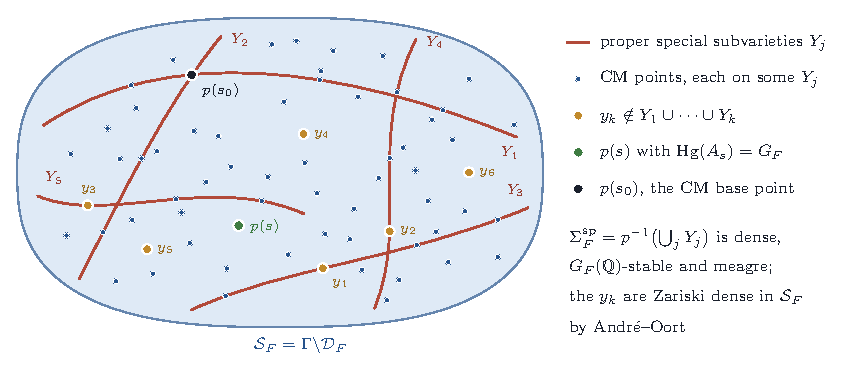
\includegraphics[width=\textwidth]{fig_speciallocus}
\caption{\Cref{prop:speciallocus} and \Cref{thm:escape} on the quotient
$\cS_{F}$. The curves are five of the countably many proper special
subvarieties $Y_{j}$, whose union is the image of the special locus; it
contains $p(s_{0})$ and is dense and meagre. The small dots are CM points,
each lying on some $Y_{j}$, drawn or not. The points $y_{1},\dots,y_{6}$
begin an escaping sequence chosen as in the proof of \Cref{thm:escape}(i):
$y_{k}$ lies on no $Y_{j}$ with $j\le k$, so $y_{1}$ may lie on $Y_{3}$ and
$y_{2}$ on $Y_{4}$. A point $p(s)$ at which the Hodge group is all of $G_{F}$
lies on none of them.}
\label{fig:speciallocus}
\end{figure}

\appendix
\section{The exterior algebra model in coordinates}\label{app:exterior}

We record in coordinates the computation behind \Cref{thm:fmtheta}, both to
pin down the sign in \eqref{eq:fmtheta} and because the programs of the
archive \cite{BMB26} use this model.

Let $g\ge1$ and let $W$ be the $\QQ$-vector space with basis
$e_{1},\dots,e_{2g},f_{1},\dots,f_{2g}$. We identify
$V=\langle e_{1},\dots,e_{2g}\rangle$ with $H^{1}(A,\QQ)$ and
$V^{\vee}=\langle f_{1},\dots,f_{2g}\rangle$ with $H^{1}(\Av,\QQ)$, so that
$\bigwedge^{*}W=H^{*}(A\times\Av,\QQ)$.

Number the generators so that the generator numbered $i$ is $e_{i}$ for
$i\le2g$ and $f_{i-2g}$ for $i>2g$. A basis of $\bigwedge^{*}W$ is then
indexed by the subsets $S$ of $\{1,\dots,4g\}$, the basis element $w_{S}$
being the wedge of the generators in $S$ in increasing order. The product
is $w_{S}w_{T}=\varepsilon(S,T)\,w_{S\cup T}$ when $S\cap T=\emptyset$ and zero
otherwise, where
\begin{equation}\label{eq:shufflesign}
  \varepsilon(S,T)=(-1)^{\#\{(s,t)\in S\times T\,:\,s>t\}} .
\end{equation}

The three distinguished elements are
\[
  \ell=\sum_{i=1}^{2g}e_{i}\wedge f_{i},
  \qquad
  \theta=\sum_{j=1}^{g}e_{j}\wedge e_{g+j},
  \qquad
  \theta'=\sum_{j=1}^{g}f_{j}\wedge f_{g+j},
\]
and $p_{*}$ is the linear map $\bigwedge^{*}W\to\bigwedge^{*}V$ that sends
$w_{S}$ to $\varepsilon(S\cap[1,2g],\,S\setminus[1,2g])\,w_{S\cap[1,2g]}$ when
$S\supseteq\{2g+1,\dots,4g\}$ and to zero otherwise.

\begin{lemma}\label{lem:appsign}
Let $0\le k\le g$, let $T\subseteq\{1,\dots,g\}$ with $|T|=k$, let
$U=\{1,\dots,g\}\setminus T$ and $S=U\cup(g+U)$. In the product
$\theta'^{\,k}\cdot e^{\ell}$ the unique term contributing $w_{S}$ after
$p_{*}$ is
\[
  k!\;\Bigl(\prod_{j\in T}f_{j}f_{g+j}\Bigr)\cdot\Bigl(\prod_{i\in S}e_{i}f_{i}\Bigr),
\]
and its image under $p_{*}$ is
$k!\,\sigma(g,k)\,\prod_{j\in U}e_{j}\wedge e_{g+j}$ with
$\sigma(g,k)=(-1)^{g(g+1)/2+k}$, independent of $T$.
\end{lemma}

\begin{proof}
The uniqueness of the term and the identification of $S$ are established in
the proof of \Cref{thm:fmtheta}. The sign is the product of the two shuffle
signs \eqref{eq:shufflesign} relating the displayed word to the target word
$\bigl(\prod_{j\in U}e_{j}e_{g+j}\bigr)\bigl(f_{1}\cdots f_{2g}\bigr)$.
Relabelling the symplectic pairs by a permutation $\pi$ of $\{1,\dots,g\}$
carries the word for $T$ to the word for $\pi(T)$ and multiplies both the
displayed and the target word by the sign of the induced permutation of
generators, so the quotient is unchanged. Since the permutations of
$\{1,\dots,g\}$ act transitively on its $k$-subsets, $\sigma$ depends only on
$(g,k)$. Evaluating at $T=\{1,\dots,k\}$, as in the proof of
\Cref{thm:fmtheta}, gives the stated value.
\end{proof}

\begin{remark}
At $g=2$ the computation can be done by hand. There
$\ell=e_{1}f_{1}+e_{2}f_{2}+e_{3}f_{3}+e_{4}f_{4}$,
$\theta=e_{1}e_{3}+e_{2}e_{4}$ and $\theta'=f_{1}f_{3}+f_{2}f_{4}$, and one
finds $\Phi_{\cP}(1)=-\tfrac12\theta^{2}$, $\Phi_{\cP}(\theta')=\theta$ and
$\Phi_{\cP}(\theta'^{2})=-2$, in agreement with \eqref{eq:fmtheta} for $g=2$,
where $(-1)^{g(g+1)/2}=(-1)^{3}=-1$.
\end{remark}

\section{The locus of Hodge classes}\label{app:cdk}

Deformation arguments about Hodge classes rest on one theorem, that of
Cattani, Deligne and Kaplan \cite{CDK95}: the locus in a family where a given
class stays a Hodge class is an algebraic subvariety, not merely an analytic
one. This appendix states the theorem, proves its elementary part, isolates
the two analytic inputs that the rest requires, computes the example that
matters here, and explains why the theorem is not a route to the Hodge
conjecture. The last point is the one that bears on \Cref{sec:construction},
and it is why the material is set out here rather than cited.

\subsection{Variations of Hodge structure}

\begin{definition}[Variation of Hodge structure]\label{def:vhs}
Let $S$ be a smooth connected complex quasi-projective variety. A
\emph{polarised variation of $\QQ$-Hodge structure} of weight $w$ on $S$
consists of
\begin{enumerate}[label=\textup{(\alph*)},nosep]
\item a local system $\mathbb{V}$ of finite dimensional $\QQ$-vector spaces on
  $S$, with associated holomorphic bundle
  $\cV=\mathbb{V}\otimes_{\QQ}\cO_{S}$ carrying the flat connection $\nabla$
  whose flat sections are $\mathbb{V}$;
\item a decreasing filtration $\cV=F^{0}\supseteq F^{1}\supseteq\cdots$ by
  holomorphic subbundles, inducing on each fibre $\mathbb{V}_{s}$ a
  $\QQ$-Hodge structure of weight $w$;
\item a flat nondegenerate $(-1)^{w}$-symmetric pairing
  $Q\colon\mathbb{V}\otimes\mathbb{V}\to\QQ_{S}$ polarising each fibre;
\end{enumerate}
subject to Griffiths transversality
\begin{equation}\label{eq:transversality}
  \nabla F^{p}\subseteq F^{p-1}\otimes\Omega^{1}_{S}.
\end{equation}
\end{definition}

The example to keep in mind is the geometric one: for $f\colon\cX\to S$ smooth
projective, $\mathbb{V}=R^{w}f_{*}\QQ$ with its Gauss--Manin connection is such
a variation, and \eqref{eq:transversality} is Griffiths' theorem
\cite[Ch.~10]{Voi02}. The other example we use is the Weil family of
\Cref{prop:weildomain} below, which is defined in the first instance by a
period domain rather than by a family of varieties, and which carries a
variation all the same.

\begin{notation}\label{not:totalspace}
Write $\cV^{\mathrm{an}}$ for the total space of $\cV$, a complex manifold
fibred over $S$ with fibre $\mathbb{V}_{s}\otimes\CC$, and
$\mathbb{V}^{\mathrm{tot}}\subset\cV^{\mathrm{an}}$ for the subset of pairs
$(s,\alpha)$ with $\alpha\in\mathbb{V}_{s}$, a covering space of $S$ with
countable fibres.
\end{notation}

\subsection{Hodge loci}

\begin{definition}\label{def:hodgelocus}
Let $\mathbb{V}$ be a polarised variation of weight $2p$ on $S$. Its
\emph{locus of Hodge classes} is
\[
  \Hdg^{p}(\mathbb{V})
  =\bigl\{(s,\alpha)\in\mathbb{V}^{\mathrm{tot}}\;:\;
     \alpha\in F^{p}\cV_{s}\bigr\}.
\]
For $N\in\QQ$ write $\Hdg^{p}_{N}$ for the part with $Q(\alpha,\alpha)=N$.
\end{definition}

By conjugation symmetry, a rational $\alpha$ of weight $2p$ lies in $F^{p}$
exactly when it is of type $(p,p)$. The following two lemmas are elementary,
and they give everything about $\Hdg^{p}$ except algebraicity.

\begin{lemma}[Analyticity]\label{lem:hodgeanalytic}
$\Hdg^{p}(\mathbb{V})$ is a closed analytic subset of
$\mathbb{V}^{\mathrm{tot}}$, and the projection
$\pi\colon\Hdg^{p}(\mathbb{V})\to S$ is locally biholomorphic onto its image on
each connected component. In particular each component is a closed analytic
subvariety of an open subset of $S$, and there are countably many components.
\end{lemma}

\begin{proof}
Work on a simply connected open $U\subseteq S$ over which $\mathbb{V}$ is
trivialised, $\mathbb{V}|_{U}\cong V_{0}\times U$ for a fixed $\QQ$-vector
space $V_{0}$. Then $\mathbb{V}^{\mathrm{tot}}|_{U}$ is the disjoint union over
$\alpha\in V_{0}$ of copies of $U$. Fix $\alpha$. The quotient
$\cV/F^{p}$ is a holomorphic vector bundle on $U$, and the image
$\bar\alpha(s)$ of the flat section $\alpha$ in $(\cV/F^{p})_{s}$ is a
holomorphic section of it. The set of $s\in U$ with $\alpha\in F^{p}\cV_{s}$
is the zero locus of $\bar\alpha$, a closed analytic subset of $U$. Taking
the union over the countable set $V_{0}$ gives the first statement, and shows
that on the sheet indexed by $\alpha$ the projection $\pi$ is the inclusion of
that zero locus into $U$, hence injective. There are countably many
components because $S$ is covered by countably many such $U$, the set $V_{0}$
is countable, and each zero locus has countably many components.
\end{proof}

\begin{lemma}[Finiteness at bounded norm]\label{lem:boundednorm}
Fix $s\in S$ and $N\in\QQ$. The set of $\alpha\in\mathbb{V}_{s}$ with
$\alpha$ of type $(p,p)$, $Q(\alpha,\alpha)=N$, and $\alpha$ in a fixed
lattice $\mathbb{V}_{s,\ZZ}$, is finite. The number of such $\alpha$ is locally
constant on each component of $\Hdg^{p}_{N}$.
\end{lemma}

\begin{proof}
Decompose $\alpha$ into its primitive parts for the Lefschetz decomposition
attached to the polarisation. On the primitive part of type $(p,p)$ in weight
$2p$ the Hodge--Riemann bilinear relations read
$(-1)^{p}\,Q(\alpha,\bbar{\alpha})>0$ for $\alpha\ne0$, so the form
$(-1)^{p}Q$ is positive definite on the real span of the primitive real
$(p,p)$-classes; the same holds on each Lefschetz summand with an alternating
sign, and the resulting form $\tilde Q$ obtained by flipping signs summand by
summand is positive definite on the whole space of real $(p,p)$-classes. The
conditions $Q(\alpha,\alpha)=N$ and $\alpha$ of type $(p,p)$ therefore confine
$\alpha$ to a compact set for $\tilde Q$, and a compact set meets a lattice in
finitely many points. The count is locally constant because the lattice and $Q$
are flat and the Hodge filtration varies continuously, so no Hodge class can
appear or disappear without its $Q$-norm changing.
\end{proof}

\begin{theorem}[Cattani, Deligne and Kaplan \cite{CDK95}]\label{thm:cdk}%
\footnote{The paper is short and the proof is not: the two inputs isolated
below, the nilpotent orbit theorem and the $\SL_{2}$-orbit theorem, carry the
weight.}
Let $S$ be a smooth complex quasi-projective variety and $\mathbb{V}$ a
polarised variation of $\ZZ$-Hodge structure of weight $2p$ on $S$. Then each
connected component of $\Hdg^{p}(\mathbb{V})$ is a closed algebraic subvariety
of $\mathbb{V}^{\mathrm{tot}}$, and its image in $S$ is a closed algebraic
subvariety of $S$.
\end{theorem}

We do not reproduce the proof, which draws on the whole asymptotic theory of
degenerating Hodge structures developed in the two preceding decades. For
families of abelian varieties the algebraicity of these loci also follows, by
a different route, from Deligne's theorem that Hodge classes on abelian
varieties are absolutely Hodge; \Cref{thm:cdk} is what carries it beyond
abelian varieties. We record where the difficulty lies and which two
theorems remove it, since the shape of the argument is what one needs in
order to judge whether a deformation argument in this area is legitimate.

By \Cref{lem:hodgeanalytic} a component $Z$ of $\Hdg^{p}$ is already a closed
analytic subvariety of an open subset of $S$, and by \Cref{lem:boundednorm} it
carries a locally constant $Q$-norm and is one sheet of a finite cover of its
image. Choose a smooth projective compactification $\bar S\supseteq S$ with
$\bar S\setminus S$ a normal crossing divisor. By Chow's theorem it is enough
to show that $Z$ extends to an analytic subvariety of $\bar S$, that is, that
$Z$ does not oscillate wildly as one approaches the boundary. This is an
asymptotic question about the Hodge filtration, and it is answered by two
theorems.

\begin{enumerate}[label=\textup{(\Alph*)},leftmargin=2.2em]
\item \emph{The nilpotent orbit theorem} of Schmid \cite{Sch73}: near a
  boundary point the period map is approximated, to exponentially small error
  in the natural coordinates, by the orbit of a nilpotent Lie algebra element
  built from the local monodromy logarithms.
\item \emph{The $\SL_{2}$-orbit theorem} in several variables, of Cattani,
  Kaplan and Schmid \cite{CKS86}: that nilpotent orbit is in turn approximated
  by an orbit of a fixed real reductive group, with uniform estimates in the
  several-variable setting.
\end{enumerate}

Together these give a two-sided estimate for the Hodge norm of a flat section
near the boundary, of the shape $\|\alpha\|_{s}\sim\prod_{j}(\log|t_{j}|^{-1})^{m_{j}}$
with integers $m_{j}$ determined by the weight filtration. A flat section that
is Hodge on $Z$ has its norm for the positive definite form $\tilde Q$ of
the proof of \Cref{lem:boundednorm} bounded by that lemma, and the
estimate converts that bound into a statement that the possible boundary
behaviours form a finite list. Algebraicity then follows from the analytic
extension across the boundary together with Chow's theorem in $\bar S$.

\begin{remark}\label{rem:cdkinputs}
Both (A) and (B) are theorems about degenerating Hodge structures, and
neither mentions algebraic cycles. The algebraicity in \Cref{thm:cdk} is
algebraicity of a locus of periods, obtained by analysis, and it carries no
information about algebraic cycles; \Cref{ssec:cdknot} develops the point.
\end{remark}

\subsection{The Weil family}

The example relevant to this paper is the family of complex structures on the
model of \Cref{setup:model}.

\begin{proposition}[The Weil period domain]\label{prop:weildomain}
Fix $K$, $n$, the $K$-space $V=K^{2n}$, and the hermitian form $H$ of
signature $(n,n)$ from \Cref{lem:hermform}. The set of Hodge structures of
weight one on $V$ that are polarised by $Q$, commute with the $K$-action, and
are of $(K,-1,n)$-Weil type is in bijection with
\[
  \cD_{n,n}
  =\bigl\{P\subset V_{+}\;:\;\dim_{\CC}P=n,\ H|_{P}\ \text{negative definite}\bigr\},
\]
an open subset of the Grassmannian $\mathrm{Gr}(n,2n)$ and a bounded symmetric
domain isomorphic to $\mathrm{U}(n,n)/\bigl(\mathrm{U}(n)\times\mathrm{U}(n)\bigr)$.
In particular
\[
  \dim_{\CC}\cD_{n,n}=n^{2},
\]
compared with $\dim\cA_{2n}=n(2n+1)$ for the moduli of principally polarised
abelian $2n$-folds.
\end{proposition}

\begin{proof}
A Hodge structure of weight one on $V$ is a subspace $V^{1,0}\subset V_{\CC}$
with $V_{\CC}=V^{1,0}\oplus\overline{V^{1,0}}$. Commuting with the $K$-action
means that $V^{1,0}$ is stable under the operator $S$ of \Cref{setup:model},
so that it splits as $V^{1,0}=P\oplus P'$ with $P=V^{1,0}\cap V_{+}$ and
$P'=V^{1,0}\cap V_{-}$.
Conjugation interchanges $V_{+}$ and $V_{-}$, so
$\overline{V^{1,0}}=\bbar{P}\oplus\bbar{P'}$ with $\bbar{P}\subset V_{-}$, and
the direct sum condition becomes $V_{-}=P'\oplus\bbar{P}$, which determines
$P'$ up to the choice of a complement; the Weil condition
$\dim P=\dim P'=n$ of \Cref{lem:balanced} together with the polarisation
condition pins it down as $P'=\bbar{P}^{\perp_{H}}$. The structure is
therefore determined by $P$.

For the positivity, extend $H$ to the $\CC$-bilinear pairing between $V_{+}$
and $V_{-}$. By the computation \eqref{eq:Qplusminus} in the proof of
\Cref{thm:model}, the second Riemann relation holds exactly when $i\,Q$ is
positive on $V^{1,0}$, and on the $V_{+}$ part this is the condition that $H$
be negative definite on $P$, the sign being fixed by the convention of
\Cref{lem:hermform}. The set of $n$-dimensional negative definite subspaces
of a hermitian space of signature $(n,n)$ is the standard realisation of the
symmetric domain of $\mathrm{U}(n,n)$: the unitary group acts transitively on
it and the stabiliser of a point is $\mathrm{U}(n)\times\mathrm{U}(n)$, the
unitary groups of $P$ and of $P^{\perp}$. It is open in $\mathrm{Gr}(n,2n)$
because negative definiteness is an open condition, and
$\dim\mathrm{Gr}(n,2n)=n(2n-n)=n^{2}$.

For the comparison, $\dim\cA_{g}=g(g+1)/2$, which is $n(2n+1)$ for $g=2n$.
\end{proof}

\begin{corollary}[The Weil locus is algebraic]\label{cor:weilalgebraic}
Inside $\cA_{2n}$ the image of $\cD_{n,n}$, that is the locus of principally
polarised abelian $2n$-folds admitting an action of an order of $K$ of
$(K,-1,n)$-Weil type, is a closed algebraic subvariety of dimension $n^{2}$.
\end{corollary}

\begin{proof}
The condition of admitting such an action is the condition that a certain
class in $\End(H^{1})$, namely the graph of $\iota(\sqrt{-d})$, be a Hodge
class, together with the balanced signature, which is locally constant. The
locus is therefore a component of a locus of Hodge classes for the variation
$\End(R^{1}f_{*}\QQ)$ over $\cA_{2n}$ with its level structure, and
\Cref{thm:cdk} applies. The dimension is \Cref{prop:weildomain}.
\end{proof}

\subsection{Limits of the theorem}\label{ssec:cdknot}

\begin{remark}[Algebraic locus, not algebraic class]\label{rem:notalgebraic}
\Cref{thm:cdk} says that the set of parameters where $\alpha$ is Hodge is cut
out by polynomial equations. It says nothing about whether $\alpha$ is the
class of a cycle at any one of those parameters. The two statements are
independent in both directions: the Hodge locus of a class that happens to be
algebraic everywhere is still known to be algebraic only through
\Cref{thm:cdk}, and conversely the algebraicity of the locus supplies no
cycle. The distinction is easily blurred, and \Cref{cor:weilalgebraic} is
exactly the kind of statement that invites it: the Weil locus is an algebraic
subvariety, even a Shimura subvariety, and none of that produces the class
$\omega_{1}$ of \eqref{eq:omegagens}. \Cref{fig:moduli} compares the
dimension of the Weil locus with that of $\cA_{2n}$.
\end{remark}

\begin{figure}[htbp]
\centering
  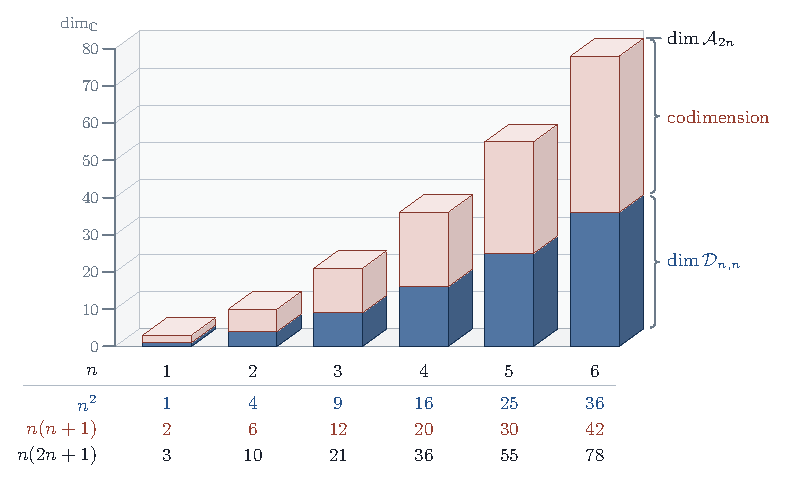
\includegraphics[width=0.92\textwidth]{fig_moduli}
\caption{The Weil locus inside the moduli of principally polarised abelian
$2n$-folds, for $n=1,\dots,6$. Each prism has the height $n(2n+1)$ of the
moduli space $\cA_{2n}$; its lower part, of height $n^{2}$, is the
dimension of the period domain $\cD_{n,n}$ of \Cref{prop:weildomain}, and
its upper part is the codimension $n(n+1)$. The codimension grows
quadratically, so the Weil locus is thin, and by \Cref{cor:weilalgebraic} it
is an algebraic subvariety. Both facts matter for propagation: the locus
along which one would have to deform is small and is a variety, but neither
fact produces a cycle on it.}
\label{fig:moduli}
\end{figure}

\begin{remark}[The variational Hodge conjecture]\label{rem:variational}
The property that would turn \Cref{thm:cdk} into a tool is the variational
Hodge conjecture of Grothendieck: if $\cX\to S$ is smooth projective over a
connected base, $\alpha$ is a flat section of $R^{2p}f_{*}\QQ$ that is Hodge at
every point, and $\alpha_{s_{0}}$ is algebraic at one point $s_{0}$, then
$\alpha_{s}$ is algebraic at every point. Its infinitesimal form is a
theorem under a semiregularity hypothesis: if the cycle at
$s_{0}$ is semiregular in the sense of Bloch \cite{Blo72}, then it deforms to
first order, and hence formally, along the locus where its class stays Hodge.
That theorem is the subject of \Cref{sec:semireg}, and
\Cref{cor:countnotbind} shows that its numerical hypothesis is not what
obstructs the present problem.
\end{remark}

\begin{remark}[The construction of
\texorpdfstring{\Cref{sec:construction}}{Section 14}]\label{rem:cdkconstruction}
The construction of \Cref{sec:construction} produces, for every $n$, every $d$
and every nondegenerate $\beta$, an abelian variety of Weil type together with
secant sheaves whose Chern classes are computed in closed form, and its output
is algebraic on the split locus. The missing ingredient, described in
\Cref{rem:deformation}, is a statement along the algebraic locus of
\Cref{cor:weilalgebraic}: the Hodge type of the deformed object has to be
controlled as the parameter moves off the split locus. \Cref{thm:cdk}
guarantees that the locus along which one deforms is an algebraic variety,
which is what makes the question well posed, but it does not answer the
question. \Cref{q:higher} states it precisely.
\end{remark}

\section{Endomorphism algebras and Weil type}\label{app:albert}

\Cref{def:weiltype} asks for three things: an even dimension, an imaginary
quadratic field acting with balanced eigenvalue multiplicities, and
compatibility with the polarisation. This appendix places these conditions
inside Albert's classification of endomorphism algebras. Two statements used
in the body come out of it. The first is that the compatibility condition is
automatic once the field is stable under the Rosati involution, so that it
reduces to that stability (\Cref{lem:rosatiauto}). The second is that the
balanced condition is not a normalisation but exactly the condition under
which the Weil line carries a Hodge class (\Cref{prop:signatureforced}); this
is why the subject concerns balanced signatures alone.

\subsection{Positive involutions}

\begin{definition}\label{def:positive}
Let $D$ be a finite dimensional semisimple $\QQ$-algebra. An involution
$\dagger$ of $D$, that is a $\QQ$-linear anti-automorphism with
$\dagger^{2}=\id$, is \emph{positive} if
\[
  \Tr_{D/\QQ}\bigl(x\,x^{\dagger}\bigr)>0
  \qquad\text{for every }x\in D,\ x\ne0,
\]
where $\Tr_{D/\QQ}$ is the trace of left multiplication on $D$ as a
$\QQ$-vector space.
\end{definition}

For an abelian variety $A$ with a polarisation $\eta$, the algebra
$D=\End^{0}(A)=\End(A)\otimes\QQ$ is semisimple and the Rosati involution
$\dagger$ attached to $\eta$ is positive \cite[Ch.~5]{BL04}. Everything below
is a statement about the pair $(D,\dagger)$.

\begin{lemma}[Totally real centre]\label{lem:totallyreal}
Let $(D,\dagger)$ be as above with $D$ a division algebra, let $F$ be the
centre of $D$ and $F_{0}=\{z\in F:z^{\dagger}=z\}$. Then $F_{0}$ is a totally
real number field.
\end{lemma}

\begin{proof}
For $z\in F_{0}$ the positivity condition reads
$\Tr_{D/\QQ}(z^{2})>0$, and $\Tr_{D/\QQ}$ restricted to $F_{0}$ is
$[D:F_{0}]\cdot\Tr_{F_{0}/\QQ}$, so $\Tr_{F_{0}/\QQ}(z^{2})>0$ for every
nonzero $z\in F_{0}$. Suppose $F_{0}$ had a complex place $\sigma$. The
embedding of $F_{0}$ into the product of its archimedean completions has dense
image, so there is $z\in F_{0}$ with $\sigma(z)$ within $\tfrac1{10}$ of $i$
and $|\rho(z)|<\varepsilon$ for every other archimedean place $\rho$. Then
$\Tr_{F_{0}/\QQ}(z^{2})=\sum_{\rho}\rho(z)^{2}$, where a complex place
contributes twice the real part of $\rho(z)^{2}$. The real part of
$\sigma(z)^{2}$ is less than $-1+\tfrac{2}{10}+\tfrac{1}{100}<-\tfrac12$, so
the term from $\sigma$ is less than $-1$, and the remaining terms are
bounded in absolute value by $2[F_{0}:\QQ]\varepsilon^{2}$, so the total is
negative for $\varepsilon$ small. This contradicts positivity, so every place
of $F_{0}$ is real.
\end{proof}

\begin{theorem}[Albert \cite{Alb34,Alb35a,Alb35b}]\label{thm:albert}%
\footnote{The numbering of the four types is Albert's and has stuck, although
it follows no natural order: types I to III have a totally real centre and
type IV a CM one, so the natural division is two against two rather than three
against one. Shimura's normalisation of the same classification, in terms of
the associated symmetric domains, is the one that makes the moduli side
transparent.}
Let $(D,\dagger)$ be a division algebra over $\QQ$ with a positive involution,
$F$ its centre, $F_{0}$ the subfield fixed by $\dagger$, $e_{0}=[F_{0}:\QQ]$
and $[D:F]=d^{2}$. Then $F_{0}$ is totally real, $[F:F_{0}]\in\{1,2\}$, and
exactly one of the following holds.
\begin{enumerate}[label=\textup{Type \Roman*.},leftmargin=4.2em,itemsep=2pt]
\item $D=F=F_{0}$ is a totally real field and $\dagger$ is the identity.
\item $F=F_{0}$ is totally real and $D$ is a quaternion algebra over $F$ with
  $D\otimes_{F,\rho}\RR\cong M_{2}(\RR)$ at every real place $\rho$;
  $\dagger$ is of orthogonal type.
\item $F=F_{0}$ is totally real and $D$ is a quaternion algebra over $F$ with
  $D\otimes_{F,\rho}\RR\cong\mathbb{H}$ at every real place $\rho$; $\dagger$
  is the canonical involution.
\item $F$ is a CM field with maximal totally real subfield $F_{0}$, and
  $\dagger$ induces complex conjugation on $F$.
\end{enumerate}
If moreover $D=\End^{0}(A)$ for an abelian variety $A$ of dimension $g$ with
$\dagger$ the Rosati involution of a polarisation, then
\[
  \text{\rm I: } e_{0}\mid g,
  \qquad
  \text{\rm II: } 2e_{0}\mid g,
  \qquad
  \text{\rm III: } 2e_{0}\mid g,
  \qquad
  \text{\rm IV: } e_{0}d^{2}\mid g .
\]
\end{theorem}

We quote \Cref{thm:albert} as a classification. \Cref{lem:totallyreal}
proves the part of it that we use directly, and the four types with their
divisibility conditions are in \cite[Ch.~9]{BL04}. \Cref{fig:albert} draws the
signatures of an imaginary quadratic action and the dimensions of their
families.

\begin{figure}[htbp]
\centering
  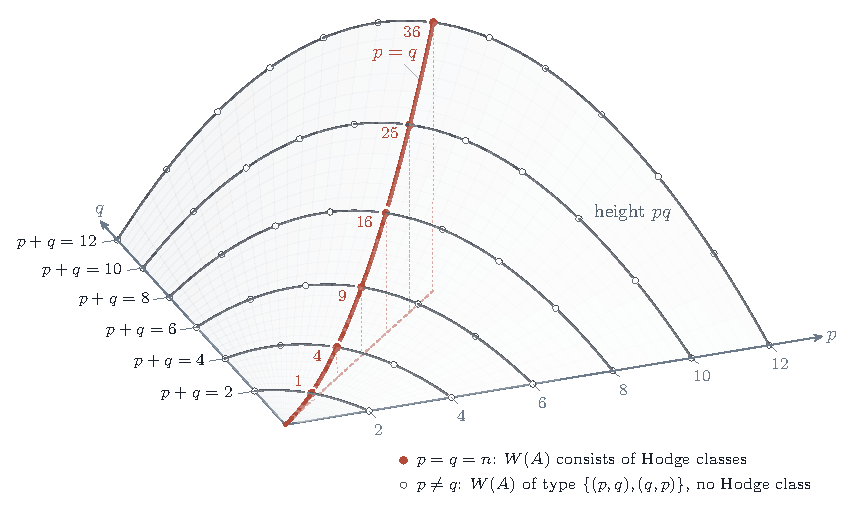
\includegraphics[width=0.92\textwidth]{fig_signature}
\caption{The signatures $(p,q)$ of an imaginary quadratic action, with
$p+q=\dim A$, drawn on the surface of height $pq$, which is the dimension of
the family of abelian varieties carrying that action, the unitary Shimura
variety of signature $(p,q)$. Each curve on the surface collects the
signatures available in one dimension, and on it the diagonal point is the
highest. The divisibility conditions of \Cref{thm:albert} put no
constraint on which of them occur when $\End^{0}(A)=K$, by
\Cref{prop:whichtypes}(i). By \Cref{prop:signatureforced} the Weil line
consists of Hodge classes exactly at the filled points on the ridge
$p=q$, and at every open point it is a rational sub-Hodge structure of type
$\{(p,2n-p),(2n-p,p)\}$ carrying no Hodge class at all. The diagonal is the
locus that \Cref{cor:weilalgebraic} shows to be an algebraic subvariety of the
moduli.}
\label{fig:albert}
\end{figure}

\subsection{Compatibility with the polarisation}

\begin{lemma}[Rosati on an imaginary quadratic subfield]\label{lem:rosatiauto}
Let $A$ be an abelian variety with a polarisation $\eta$ and Rosati involution
$\dagger$, and let $\iota\colon K\hookrightarrow\End^{0}(A)$ be an embedding of
an imaginary quadratic field such that $\iota(K)$ is stable under $\dagger$.
Then
\[
  \iota(\tau)^{\dagger}=\iota(\bbar{\tau})
  \qquad\text{for every }\tau\in K .
\]
That is, condition \textup{(iii)} of \Cref{def:weiltype} holds automatically,
and Weil type is the conjunction of \textup{(i)}, \textup{(ii)} and the
$\dagger$-stability of $\iota(K)$.
\end{lemma}

\begin{proof}
Put $D=\End^{0}(A)$. By stability, $\dagger$ restricts to an involutive
anti-automorphism of the field $\iota(K)\cong K$. An anti-automorphism of a
commutative ring is an automorphism, and $\Gal(K/\QQ)$ has order two, so the
restriction is either the identity or complex conjugation. Suppose it were
the identity, and put $x=\iota(\sqrt{-d})$. Then
$x\,x^{\dagger}=x^{2}=\iota(-d)=-d\cdot 1$, so
\[
  \Tr_{D/\QQ}\bigl(x\,x^{\dagger}\bigr)=-d\cdot\dim_{\QQ}D<0,
\]
contradicting the positivity of $\dagger$. Hence $\dagger$ restricts to complex
conjugation.
\end{proof}

\begin{remark}\label{rem:whystable}
Stability is a real hypothesis: a subfield of $\End^{0}(A)$ need not be
$\dagger$-stable. What \Cref{lem:rosatiauto} removes is the second half of the
condition, the identification of $\dagger|_{K}$ with a specific automorphism.
In particular, in the model of \Cref{setup:model} the polarisation need not be
chosen to match the field, since any $\dagger$-stable embedding does the same
work.
\end{remark}

\subsection{The balanced signature}

\begin{definition}[Signature]\label{def:signature}
Let $\iota\colon K\hookrightarrow\End^{0}(A)$ be as above, $g=\dim A$. The
operator $\iota(\sqrt{-d})$ acts on the tangent space $T_{0}A\cong\CC^{g}$ with
the two eigenvalues $\pm i\sqrt{d}$; write $p$ and $q=g-p$ for their
multiplicities. The pair $(p,q)$ is the \emph{signature} of $(A,\iota)$.
\end{definition}

The signature is an isogeny invariant, since an isogeny induces an isomorphism
on tangent spaces commuting with the action. It is locally constant in
families: the two eigenspaces are the kernels of
$\iota(\sqrt{-d})\mp i\sqrt{d}$ on the relative tangent bundle, so their
dimensions are upper semicontinuous, and they sum to $g$. By
duality $\iota(\tau)^{*}$ acts on $H^{1,0}(A)$ with the same multiplicities, so
$\dim V^{1,0}_{+}=p$ and $\dim V^{1,0}_{-}=q$ in the notation of
\Cref{sec:weiltype}.

\begin{proposition}[The balanced signature is forced]\label{prop:signatureforced}
Let $A$ be an abelian variety of dimension $2n$ with a $\dagger$-stable
embedding $\iota\colon K\hookrightarrow\End^{0}(A)$ of signature $(p,q)$,
$p+q=2n$, and let
\[
  \HW(A)=\Bigl(\textstyle\bigwedge^{2n}_{\CC}V_{+}
   \oplus\bigwedge^{2n}_{\CC}V_{-}\Bigr)\cap H^{2n}(A,\QQ)
\]
as in \Cref{def:weilline}. Then $\HW(A)$ is a rational sub-Hodge structure of
$H^{2n}(A,\QQ)$ of dimension two and of Hodge type
$\{(p,2n-p),\,(2n-p,p)\}$, and the following are equivalent:
\begin{enumerate}[label=\textup{(\roman*)},nosep]
\item $p=q=n$, that is $(A,\iota,\eta)$ is of $(K,-1,n)$-Weil type;
\item $\HW(A)$ contains a nonzero Hodge class;
\item $\HW(A)$ consists of Hodge classes.
\end{enumerate}
\end{proposition}

\begin{proof}
The space $\bigwedge^{2n}V_{+}$ is a line, and by \eqref{eq:bisplit} it equals
$\bigwedge^{p}V^{1,0}_{+}\otimes\bigwedge^{2n-p}V^{0,1}_{+}$, which is of pure
Hodge bidegree $(p,2n-p)$; the conjugate line $\bigwedge^{2n}V_{-}$ is of
bidegree $(2n-p,p)$. Their sum is stable under conjugation and defined over
$\QQ$ by the argument of \Cref{prop:weilline}(i), which does not use the
balanced condition, so $\HW(A)$ is a two-dimensional rational sub-Hodge
structure of the stated type.

A Hodge class is an element of bidegree $(n,n)$. A nonzero element of
$\HW(A)\otimes\CC$ has a nonzero component in one of the two lines, so it is of
bidegree $(n,n)$ only if $(p,2n-p)=(n,n)$ or $(2n-p,p)=(n,n)$, and either
equality says $p=n$. This proves that (ii) implies (i). If $p=n$ then both
lines are of bidegree $(n,n)$ and every element of $\HW(A)$ is a Hodge class,
so (i) implies (iii); and (iii) implies (ii) because $\dim\HW(A)=2>0$.
\end{proof}

\begin{remark}\label{rem:onlybalanced}
\Cref{prop:signatureforced} is the reason the literature speaks of abelian
varieties of Weil type rather than of imaginary quadratic multiplication in
general. For an unbalanced signature the space $\HW(A)$ is still a canonical
two-dimensional rational sub-Hodge structure, and it is still not in the
divisor subring, but it contains no Hodge class and therefore predicts
nothing. The exceptional Hodge classes appear exactly at balance, and the
locus of balance is the algebraic subvariety of \Cref{cor:weilalgebraic}.
\end{remark}

\subsection{Endomorphism algebras of Weil type}

\begin{proposition}[Weil type in the classification]\label{prop:whichtypes}
Let $A$ be an abelian variety of dimension $2n$ admitting a $\dagger$-stable
embedding of an imaginary quadratic field $K$ with balanced signature, and
suppose $\End^{0}(A)$ is a division algebra $D$ with centre $F$ as in
\Cref{thm:albert}. Then:
\begin{enumerate}[label=\textup{(\roman*)},nosep]
\item if $D=K$ then $D$ is of type IV with $e_{0}=1$ and $d=1$, and the
  divisibility condition of \Cref{thm:albert} is vacuous, so every even
  dimension occurs;
\item the classification does not exclude type III with $F_{0}=\QQ$: a
  totally definite quaternion algebra over $\QQ$ contains imaginary
  quadratic subfields on which the canonical involution is conjugation;
\item $D$ is not of type I, because a totally real field contains no
  imaginary quadratic subfield.
\end{enumerate}
\end{proposition}

\begin{proof}
(i) If $D=K$ then $F=K$ is a CM field with $F_{0}=\QQ$, so $e_{0}=1$; and
$[D:F]=1$ gives $d=1$. The involution is conjugation by
\Cref{lem:rosatiauto}, which is type IV. The condition $e_{0}d^{2}\mid g$ reads
$1\mid 2n$.

(ii) Let $D$ be a quaternion algebra over $\QQ$ ramified at the infinite place,
with standard generators $u,v$ satisfying $u^{2}=a<0$, $v^{2}=b<0$, $uv=-vu$,
and canonical involution $x\mapsto\bbar{x}$ fixing $\QQ$ and negating
$u,v,uv$. Then $\QQ(u)\cong\QQ(\sqrt{a})$ is imaginary quadratic, stable under
the involution, and the involution restricts to conjugation on it. Whether
such a $D$ occurs as $\End^{0}(A)$ together with a balanced signature
is a separate question about the moduli, but nothing in the classification
excludes it.

(iii) is immediate, since a totally real field has no element of negative
square.
\end{proof}

\begin{remark}[The generic case]\label{rem:genericcase}
Case (ii) of \Cref{prop:whichtypes} is a special position: there
$\End^{0}(A)$ is larger than $K$, the Hodge group is correspondingly smaller,
and $\Hdg^{n}(A)$ can be larger than the three dimensions of
\Cref{thm:hdgcount}. It is also a case in which the Weil classes can become
accessible: \cite[Remark~2.5]{paperIII} records that at such points the Weil line can
meet the divisor subring, which is the split situation. The hard case, and the
one addressed throughout \Cref{sec:divisor,sec:characters,sec:hyperplane}, is
case (i) with $\Hg(A)=\SU(V,H)$.
\end{remark}

\begin{remark}[Dimension four]\label{rem:dimfour}
For $n=1$ the Weil line lies in $H^{2}(A,\QQ)$ and consists of divisor
classes, algebraic by the Lefschetz theorem on $(1,1)$ classes, so it predicts
nothing new; this is the same boundary as in \Cref{prop:normpart}. Moonen and
Zarhin determined the Hodge classes on abelian varieties of dimension at most
five \cite{MZ99}, and on simple abelian fourfolds in \cite{MZ95}: through
dimension three the Hodge ring is generated by divisor classes, and the first
Hodge classes not of that form occur in dimension four, on abelian fourfolds of
Weil type. Thus $n=2$ is at once the first case of \Cref{def:weiltype} with
exceptional Hodge classes, the first case where \Cref{thm:hdgcount} gives
three rather than one, and the first case of the Hodge conjecture for
abelian varieties that needed more than divisor classes; Markman settled it
\cite[Corollary 1.6.1]{Mar25a}. The next case is $n=3$ with nontrivial
discriminant, by \cite[Proposition~2.12(ii)]{paperIII}.
\end{remark}


% \zenodoCodeID is the DOI the paper cites for the archive of the earlier
% paper on Weil classes, in the data availability section and in the entry
% BMB26 of the bibliography: the version DOI of release v5.0.1 of that
% archive, a version of the concept record 10.5281/zenodo.22950275.
\newcommand{\zenodoCodeID}{10.5281/zenodo.23225483}
\newcommand{\zenodoCodeDOI}{%
  \href{https://doi.org/\zenodoCodeID}{\texttt{\zenodoCodeID}}}

\section*{Acknowledgements}
The paper builds on the theorems of Eyal Markman on secant sheaves and Weil
classes, on the semiregularity theory of Spencer Bloch, Ragnar-Olaf
Buchweitz and Hubert Flenner, and on the descriptions of Hodge classes on
abelian varieties by Ben Moonen, Yuri Zarhin, Yves Andr\'e and James Milne.
We thank Priyabrata Mandal for the collaboration on the earlier paper on
Weil classes, whose results this paper and its companions \cite{paperII,paperIII} divide between them.

\section*{Declarations}

\subsection*{Funding}
The authors received no funding for this work.

\subsection*{Competing interests}
The authors have no competing interests to declare.

\subsection*{Ethics approval and consent}
This article reports no research involving human participants, human data or
animals, so ethics approval and consent to participate or to publish were not
required. The results are original and have not been published elsewhere
except in the earlier paper named on the title page, which this paper and its
companions replace, and the work of others is credited by citation throughout.

\subsection*{Data availability}
The archive \cite{BMB26} is deposited on Zenodo under the DOI
\zenodoCodeDOI. It holds programs that repeat much of the finite arithmetic of this paper and its companions \cite{paperII,paperIII}
as an independent check, a Lean~4 certificate of part of that arithmetic, the
Macaulay2 computations of local $\Ext$ algebras with their output, and the
generators and TikZ sources of the figures; its programs perform $2218$
checks, all of which pass, and the Lean kernel checks four hundred and nine
theorems, each depending on no axiom or on propositional extensionality
alone. Deep Bhattacharjee computed all the calculations, in C, Python, Julia,
Macaulay2, Lean~4 and shell scripts, with the assistance of Claude Code, an
AI model developed by Anthropic. The archive is immutable at that DOI;
the command \texttt{python3 code/verify\_all.py} in it runs every check and
ends with their count, and \texttt{lean HodgeObstruction.lean} in its folder
\texttt{lean} checks the certificate and prints the axioms of each theorem.
The Lean theorems certify finite arithmetic only: rank certificates,
enumerations, lattice computations and polynomial identities; no geometric
argument of the three papers is formalised, and every proof in the text was
written and checked by the authors. The authors are responsible for the
mathematical statements and their proofs. The \LaTeX{} source of this paper is
archived on Zenodo under the DOI \href{https://doi.org/10.5281/zenodo.23885230}{\texttt{10.5281/zenodo.23885230}}.
No other data were generated or analysed.


\begin{thebibliography}{99}

\bibitem[Alb34]{Alb34}
A. A. Albert,
\emph{On the construction of Riemann matrices. I},
Ann. of Math. (2) \textbf{35} (1934), no.~1, 1--28.
\href{https://doi.org/10.2307/1968116}{\texttt{doi:10.2307/1968116}}.

\bibitem[Alb35a]{Alb35a}
A. A. Albert,
\emph{On the construction of Riemann matrices. II},
Ann. of Math. (2) \textbf{36} (1935), no.~2, 376--394.
\href{https://doi.org/10.2307/1968578}{\texttt{doi:10.2307/1968578}}.

\bibitem[Alb35b]{Alb35b}
A. A. Albert,
\emph{Involutorial simple algebras and real Riemann matrices},
Ann. of Math. (2) \textbf{36} (1935), no.~4, 886--964.
\href{https://doi.org/10.2307/1968595}{\texttt{doi:10.2307/1968595}}.

\bibitem[And96a]{And96}
Y. Andr\'e,
\emph{On the Shafarevich and Tate conjectures for hyperk\"ahler varieties},
Math. Ann. \textbf{305} (1996), no.~1, 205--248.
\href{https://doi.org/10.1007/BF01444219}{\texttt{doi:10.1007/BF01444219}}.

\bibitem[BB26]{BB26}
D. Bhattacharjee and U. Bhattacharya,
\emph{Relative secant cycles and Hodge classes},
Preprints.org, version 5, 2026.
\href{https://doi.org/10.20944/preprints202602.0462.v5}{\texttt{doi:10.20944/preprints202602.0462.v5}}.

\bibitem[BB66]{BB66}
W. L. Baily, Jr. and A. Borel,
\emph{Compactification of arithmetic quotients of bounded symmetric domains},
Ann. of Math. (2) \textbf{84} (1966), no.~3, 442--528.
\href{https://doi.org/10.2307/1970457}{\texttt{doi:10.2307/1970457}}.

\bibitem[BF03]{BF03}
R.-O. Buchweitz and H. Flenner,
\emph{A semiregularity map for modules and applications to deformations},
Compositio Math. \textbf{137} (2003), no.~2, 135--210.
\href{https://doi.org/10.1023/A:1023999012081}{\texttt{doi:10.1023/A:1023999012081}}.

\bibitem[BF08]{BF08}
R.-O. Buchweitz and H. Flenner,
\emph{The global decomposition theorem for Hochschild (co-)homology of
singular spaces via the Atiyah--Chern character},
Adv. Math. \textbf{217} (2008), no.~1, 243--281.
\href{https://doi.org/10.1016/j.aim.2007.06.013}{\texttt{doi:10.1016/j.aim.2007.06.013}}.

\bibitem[BL04]{BL04}
C. Birkenhake and H. Lange,
\emph{Complex Abelian Varieties}, 2nd ed.,
Grundlehren der mathematischen Wissenschaften \textbf{302},
Springer, Berlin, 2004.
\href{https://doi.org/10.1007/978-3-662-06307-1}{\texttt{doi:10.1007/978-3-662-06307-1}}.

\bibitem[Blo72]{Blo72}
S. Bloch,
\emph{Semi-regularity and de Rham cohomology},
Invent. Math. \textbf{17} (1972), 51--66.
\href{https://doi.org/10.1007/BF01390023}{\texttt{doi:10.1007/BF01390023}}.

\bibitem[BMB26]{BMB26}
D. Bhattacharjee, P. Mandal and U. Bhattacharya,
\emph{Verification code and figure sources for the paper ``Algebraic Loci of
Weil Classes on Abelian Varieties''}, software archive with a Lean~4
certificate, release 5.0.1, Zenodo, 2026.
\href{https://doi.org/\zenodoCodeID}{\texttt{doi:\zenodoCodeID}}.

\bibitem[Cal05]{Cal05}
A. C\u{a}ld\u{a}raru,
\emph{The Mukai pairing, II: the Hochschild--Kostant--Rosenberg isomorphism},
Adv. Math. \textbf{194} (2005), no.~1, 34--66.
\href{https://doi.org/10.1016/j.aim.2004.05.012}{\texttt{doi:10.1016/j.aim.2004.05.012}}.

\bibitem[CDK95]{CDK95}
E. Cattani, P. Deligne and A. Kaplan,
\emph{On the locus of Hodge classes},
J. Amer. Math. Soc. \textbf{8} (1995), no.~2, 483--506.
\href{https://doi.org/10.1090/S0894-0347-1995-1273413-2}{\texttt{doi:10.1090/S0894-0347-1995-1273413-2}}.

\bibitem[CKS86]{CKS86}
E. Cattani, A. Kaplan and W. Schmid,
\emph{Degeneration of Hodge structures},
Ann. of Math. (2) \textbf{123} (1986), no.~3, 457--535.
\href{https://doi.org/10.2307/1971333}{\texttt{doi:10.2307/1971333}}.

\bibitem[Del72]{Del72}
P. Deligne,
\emph{La conjecture de Weil pour les surfaces $K3$},
Invent. Math. \textbf{15} (1972), 206--226.
\href{https://doi.org/10.1007/BF01404126}{\texttt{doi:10.1007/BF01404126}}.

\bibitem[Del82]{Del82}
P. Deligne,
\emph{Hodge cycles on abelian varieties} (notes by J. S. Milne),
in: Hodge Cycles, Motives, and Shimura Varieties,
Lecture Notes in Math. \textbf{900}, Springer, Berlin, 1982, pp.~9--100.
\href{https://doi.org/10.1007/978-3-540-38955-2_3}%
{\texttt{doi:10.1007/978-3-540-38955-2\_3}}.

\bibitem[FF26]{FF26}
S. Floccari and L. Fu,
\emph{The Hodge conjecture for Weil fourfolds with discriminant $1$ via
singular OG6-varieties},
J. Math. Pures Appl. (9) \textbf{210} (2026), paper no.~103876.
\href{https://doi.org/10.1016/j.matpur.2026.103876}{\texttt{doi:10.1016/j.matpur.2026.103876}}.

\bibitem[Ful98]{Ful98}
W. Fulton,
\emph{Intersection Theory}, 2nd ed.,
Ergebnisse der Mathematik und ihrer Grenzgebiete (3) \textbf{2},
Springer, New York, 1998.
\href{https://doi.org/10.1007/978-1-4612-1700-8}{\texttt{doi:10.1007/978-1-4612-1700-8}}.

\bibitem[GP98]{GP98}
M. Gross and S. Popescu,
\emph{Equations of $(1,d)$-polarized abelian surfaces},
Math. Ann. \textbf{310} (1998), no.~2, 333--377.
\href{https://doi.org/10.1007/s002080050151}{\texttt{doi:10.1007/s002080050151}}.

\bibitem[Gro61]{Gro61}
A. Grothendieck,
\emph{Techniques de construction et th\'eor\`emes d'existence en g\'eom\'etrie
alg\'ebrique IV: les sch\'emas de Hilbert},
S\'eminaire Bourbaki, Vol.~6 (1960/61), Exp. No.~221, 249--276;
reprinted by Soc. Math. France, Paris, 1995.

\bibitem[HM73]{HM73}
G. Horrocks and D. Mumford,
\emph{A rank $2$ vector bundle on $\mathbf{P}^{4}$ with $15{,}000$ symmetries},
Topology \textbf{12} (1973), 63--81.
\href{https://doi.org/10.1016/0040-9383(73)90022-0}{\texttt{doi:10.1016/0040-9383(73)90022-0}}.

\bibitem[Kle68]{Kle68}
S. L. Kleiman,
\emph{Algebraic cycles and the Weil conjectures},
in: Dix expos\'es sur la cohomologie des sch\'emas,
North-Holland, Amsterdam, 1968, pp.~359--386.

\bibitem[Kle94]{Kle94}
S. L. Kleiman,
\emph{The standard conjectures},
in: Motives (Seattle, WA, 1991),
Proc. Sympos. Pure Math. \textbf{55}, Part 1,
Amer. Math. Soc., Providence, RI, 1994, pp.~3--20.
\href{https://doi.org/10.1090/pspum/055.1/1265519}{\texttt{doi:10.1090/pspum/055.1/1265519}}.

\bibitem[KOU23]{KOU}
B. Klingler, A. Otwinowska and D. Urbanik,
\emph{On the fields of definition of Hodge loci},
Ann. Sci. \'Ec. Norm. Sup\'er. (4) \textbf{56} (2023), no.~4, 1299--1312.
\href{https://doi.org/10.24033/asens.2555}{\texttt{doi:10.24033/asens.2555}}.

\bibitem[KS67]{KS67}
M. Kuga and I. Satake,
\emph{Abelian varieties attached to polarized $K3$-surfaces},
Math. Ann. \textbf{169} (1967), 239--242.
\href{https://doi.org/10.1007/BF01399540}{\texttt{doi:10.1007/BF01399540}}.

\bibitem[Mar25a]{Mar25a}
E. Markman,
\emph{Cycles on abelian $2n$-folds of Weil type from secant sheaves on abelian
$n$-folds}, preprint, arXiv:2502.03415 (2025).
\href{https://doi.org/10.48550/arXiv.2502.03415}{\texttt{doi:10.48550/arXiv.2502.03415}}.

\bibitem[Mar25b]{Mar25b}
E. Markman,
\emph{Secant sheaves and Weil classes on abelian varieties},
preprint, arXiv:2509.23403 (2025).
\href{https://doi.org/10.48550/arXiv.2509.23403}{\texttt{doi:10.48550/arXiv.2509.23403}}.

\bibitem[Mar25c]{Mar25c}
E. Markman,
\emph{Secant sheaves on abelian $n$-folds with real multiplication and Weil
classes on abelian $2n$-folds with complex multiplication},
preprint, 2025.
\href{https://arxiv.org/abs/2509.23079}{\texttt{arXiv:2509.23079}}.

\bibitem[Muk81]{Muk81}
S. Mukai,
\emph{Duality between $D(X)$ and $D(\hat{X})$ with its application to Picard
sheaves},
Nagoya Math. J. \textbf{81} (1981), 153--175.
\href{https://doi.org/10.1017/S002776300001922X}{\texttt{doi:10.1017/S002776300001922X}}.

\bibitem[MZ95]{MZ95}
B. Moonen and Yu. G. Zarhin,
\emph{Hodge classes and Tate classes on simple abelian fourfolds},
Duke Math. J. \textbf{77} (1995), no.~3, 553--581.
\href{https://doi.org/10.1215/S0012-7094-95-07717-5}{\texttt{doi:10.1215/S0012-7094-95-07717-5}}.

\bibitem[MZ99]{MZ99}
B. Moonen and Yu. G. Zarhin,
\emph{Hodge classes on abelian varieties of low dimension},
Math. Ann. \textbf{315} (1999), no.~4, 711--733.
\href{https://doi.org/10.1007/s002080050333}{\texttt{doi:10.1007/s002080050333}}.

\bibitem[II]{paperII}
D. Bhattacharjee and U. Bhattacharya,
\emph{Secant objects for Weil classes on abelian varieties},
companion to the present paper, preprint (2026).

\bibitem[III]{paperIII}
D. Bhattacharjee and U. Bhattacharya,
\emph{Hodge classes beyond the Weil lines},
companion to the present paper, preprint (2026).

\bibitem[PR94]{PR94}
V. P. Platonov and A. S. Rapinchuk,
\emph{Algebraic Groups and Number Theory},
Pure and Applied Mathematics \textbf{139},
Academic Press, Boston, MA, 1994.

\bibitem[Pri24]{Pri24}
J. P. Pridham,
\emph{Semiregularity as a consequence of Goodwillie's theorem},
Forum Math. Sigma \textbf{12} (2024), e126. arXiv:1208.3111.
\href{https://doi.org/10.1017/fms.2024.132}{\texttt{doi:10.1017/fms.2024.132}}.

\bibitem[PST21]{PST}
J. Pila, A. N. Shankar and J. Tsimerman,
\emph{Canonical heights on Shimura varieties and the Andr\'e--Oort
conjecture}, with an appendix by H. Esnault and M. Groechenig,
preprint, arXiv:2109.08788 (2021).
\href{https://doi.org/10.48550/arXiv.2109.08788}{\texttt{doi:10.48550/arXiv.2109.08788}}.

\bibitem[Sat66]{Sat66}
I. Satake,
\emph{Clifford algebras and families of abelian varieties},
Nagoya Math. J. \textbf{27} (1966), 435--446.
\href{https://doi.org/10.1017/S0027763000026295}{\texttt{doi:10.1017/S0027763000026295}}.

\bibitem[Sch73]{Sch73}
W. Schmid,
\emph{Variation of Hodge structure: the singularities of the period mapping},
Invent. Math. \textbf{22} (1973), 211--319.
\href{https://doi.org/10.1007/BF01389674}{\texttt{doi:10.1007/BF01389674}}.

\bibitem[Sch85]{Sch85}
W. Scharlau,
\emph{Quadratic and Hermitian Forms},
Grundlehren der mathematischen Wissenschaften \textbf{270},
Springer, Berlin, 1985.
\href{https://doi.org/10.1007/978-3-642-69971-9}{\texttt{doi:10.1007/978-3-642-69971-9}}.

\bibitem[Sch98]{Sch98}
C. Schoen,
\emph{Addendum to: Hodge classes on self-products of a variety with an
automorphism},
Compositio Math. \textbf{114} (1998), no.~3, 329--336.
\href{https://doi.org/10.1023/A:1000566205021}{\texttt{doi:10.1023/A:1000566205021}}.

\bibitem[Tot26]{Tot26}
B. Totaro,
\emph{On the Hodge conjecture},
guest post on the weblog of T. Tao, 11 September 2026.
\href{https://terrytao.wordpress.com/2026/09/11/on-the-hodge-conjecture/}%
{\texttt{terrytao.wordpress.com/2026/09/11/on-the-hodge-conjecture}}.

\bibitem[Tsi18]{Tsi18}
J. Tsimerman,
\emph{The Andr\'e--Oort conjecture for $\mathcal{A}_{g}$},
Ann. of Math. (2) \textbf{187} (2018), no.~2, 379--390.
\href{https://doi.org/10.4007/annals.2018.187.2.2}{\texttt{doi:10.4007/annals.2018.187.2.2}}.

\bibitem[vG00]{vG00}
B. van Geemen,
\emph{Kuga--Satake varieties and the Hodge conjecture},
in: The Arithmetic and Geometry of Algebraic Cycles (Banff, 1998),
NATO Sci. Ser. C Math. Phys. Sci. \textbf{548},
Kluwer, Dordrecht, 2000, pp.~51--82.
\href{https://doi.org/10.1007/978-94-011-4098-0_3}{\texttt{doi:10.1007/978-94-011-4098-0\_3}}.

\bibitem[Voi02]{Voi02}
C. Voisin,
\emph{Hodge Theory and Complex Algebraic Geometry I},
Cambridge Studies in Advanced Mathematics \textbf{76},
Cambridge University Press, Cambridge, 2002.
\href{https://doi.org/10.1017/CBO9780511615344}{\texttt{doi:10.1017/CBO9780511615344}}.

\bibitem[Voi03]{Voi03}
C. Voisin,
\emph{Hodge Theory and Complex Algebraic Geometry II},
Cambridge Studies in Advanced Mathematics \textbf{77},
Cambridge University Press, Cambridge, 2003.
\href{https://doi.org/10.1017/CBO9780511615177}{\texttt{doi:10.1017/CBO9780511615177}}.

\bibitem[Voi26]{Voi26}
C. Voisin,
\emph{The status of the Hodge conjecture},
guest post on the weblog of T. Tao, 12 September 2026.
\href{https://terrytao.wordpress.com/2026/09/12/the-status-of-the-hodge-conjecture/}%
{\texttt{terrytao.wordpress.com/2026/09/12/the-status-of-the-hodge-conjecture}}.

\bibitem[Wei77]{Weil77}
A. Weil,
\emph{Abelian varieties and the Hodge ring},
in: \OE uvres Scientifiques, Collected Papers, Vol.~III,
Springer, New York, 1979, pp.~421--429.

\end{thebibliography}


\end{document}
